\documentclass[11pt,a4paper,twoside,openany]{book}
\usepackage{lifeos}
\usepackage{pgfplots}\pgfplotsset{compat=1.17}
\usepackage{circuitikz}
\usepackage{graphicx}
\usepackage[font=small,labelfont=bf]{caption}
\usepackage{subcaption}
\usepackage{makeidx}\makeindex
\usetikzlibrary{positioning}
\setlifeostitle{BOOK TITLE}
\setcounter{tocdepth}{1}

\begin{document}
\frontmatter
\pagestyle{empty}
\makecover{BOOK TITLE}{Subtitle}{Study textbook}
\newpage\pagestyle{fancy}
\tableofcontents
\chapter*{Start here: from zero}
\addcontentsline{toc}{chapter}{Start here: from zero}
\markboth{Start here}{Start here}

This book starts at the point where school algebra ends, and ends at the
mathematics inside a working machine-learning library. If you can solve two
equations in two unknowns, you can begin. This chapter explains what ``linear
algebra'' is for, fixes the notation, and gives the single-variable calculus
needed for Chapter~11, so that nothing later arrives unannounced.

\section*{Why this subject exists}

A spreadsheet row of numbers is a \emph{vector}. A spreadsheet is a \emph{matrix}.
A rule that turns one row into another by multiplying and adding --- a
photo filter, a currency conversion, one layer of a neural network --- is a
\emph{linear map}. Linear algebra is the study of these objects, and it is useful
because the same few ideas (solve a system, find the best fit, find the
important directions) show up in every field that handles data.

\section*{A system of equations, from school}

Solve $2x - y = 0$ and $-x + 2y = 3$ by substitution. The first equation gives
$y=2x$. Putting that into the second: $-x+2(2x)=3$, so $3x=3$, so $x=1$ and $y=2$.
Check: $2(1)-2=0$ and $-1+2(2)=3$. Chapter~1 solves this same system two other
ways and then solves systems with hundreds of unknowns, where substitution would
be hopeless.

\section*{The notation, in one page}

\begin{center}
\begin{tabular}{lP{9.2cm}}
\toprule
\thead{Symbol} & \thead{Meaning}\\
\midrule
$\mathbb R$ & the real numbers, i.e.\ the number line\\
$\mathbb R^{n}$ & lists of $n$ real numbers; $\mathbb R^{2}$ is the plane, $\mathbb R^{3}$ is space\\
$\mathbf x$ & a vector, written as a column, such as $\begin{pmatrix}1\\2\end{pmatrix}$\\
$A$ & a matrix, a rectangular table; $A$ is $m\times n$ if it has $m$ rows and $n$ columns\\
$a_{ij}$ & the entry of $A$ in row $i$, column $j$\\
$A^{\mathsf T}$ & the transpose: swap rows and columns\\
$\sum_{i=1}^{n}a_i$ & $a_1+a_2+\dots+a_n$\\
$\in$ & ``is an element of''; $\mathbf x\in\mathbb R^{3}$ says $\mathbf x$ is a list of three numbers\\
$\forall$, $\exists$ & ``for every'', ``there exists''\\
\bottomrule
\end{tabular}
\end{center}

\section*{A calculus primer for Chapter~11}

You will not need calculus until Chapter~11, but it is better to meet it here.
The \emph{derivative} $f'(x)$ of a function $f$ is the slope of its graph at $x$:
how fast $f$ changes when $x$ is nudged. For example $f(x)=x^2$ has $f'(x)=2x$;
at $x=3$ the slope is $6$, so a nudge of $0.01$ raises $f$ by about $0.06$
(indeed $3.01^2-3^2=0.0601$). The \emph{chain rule} handles a function inside a
function: if $f(x)=(3x+1)^2$ then $f'(x)=2(3x+1)\cdot 3=18x+6$, the derivative of
the outside evaluated at the inside, times the derivative of the inside. You can
confirm by expanding $(3x+1)^2=9x^2+6x+1$ and differentiating directly.
Chapter~11 extends exactly these two ideas to functions of many variables.

\section*{How the books of this series fit together}

This is Book~3 of eight, and it is the mathematical spine of the data half of the
series.

\begin{center}
\begin{tabular}{P{2.4cm}P{9.0cm}}
\toprule
\thead{Book} & \thead{Connection}\\
\midrule
2 Discrete maths & Teaches how to read and write proofs; this book states each theorem and then proves it in that style. Chapter~12 here builds on its finite probability.\\
4 Machine learning & Cites this book by chapter: least squares (Chapter~8), PCA (Chapter~10), gradients and backpropagation (Chapters~11 and~14), losses (Chapter~15).\\
6 Quant research & Uses the statistics of Chapter~13 and the covariance ideas of Chapters~9--10.\\
\bottomrule
\end{tabular}
\end{center}

\section*{How to use the boxes in each chapter}

Every chapter opens with \emph{After this chapter you can}, listing concrete
skills. From Chapter~2, a \emph{Before you start} box names the earlier
chapters it relies on and gives a one-sentence recap, so you can tell whether to
reread something. Each chapter ends with a \emph{Hand derivation} section: do it
on paper before you trust the code.

\mainmatter
\chapter{Linear systems and Gaussian elimination}\label{ch:elimination}

Nearly every computation in this book — least squares, eigenvalue computations, and the neural-network training of part~IV — ends with a system of linear equations. This chapter builds the one algorithm that solves them honestly: Gaussian elimination. After it you will be able to (a) read a linear system two ways, as intersecting hyperplanes and as a combination of columns; (b) reduce any system to echelon form and read off whether it has zero, one, or infinitely many solutions; (c) package the work of elimination as the factorization $PA=LU$; and (d) say why elimination costs about $n^3$ operations and why a naive computer must swap rows to stay accurate.

\section{Two ways to see \texorpdfstring{$A\mathbf{x}=\mathbf{b}$}{Ax = b}}\label{sec:rowcol}

A \emph{linear system}\index{linear system} is a set of equations
\[
  a_{11}x_1 + a_{12}x_2 + \cdots + a_{1n}x_n = b_1,
  \quad\ldots\quad
  a_{m1}x_1 + a_{m2}x_2 + \cdots + a_{mn}x_n = b_m,
\]
which we compress into $A\mathbf{x}=\mathbf{b}$: the \emph{coefficient matrix}\index{coefficient matrix} $A$ is $m\times n$, $\mathbf{x}$ is the unknown column vector in $\mathbb{R}^n$, and $\mathbf{b}\in\mathbb{R}^m$ is given. Take the smallest non-trivial case, $m=n=2$:
\[
  2x - y = 0, \qquad -x + 2y = 3.
\]
There are two honest ways to look at it, and you need both.

\begin{description}
  \item[Row picture.] Each equation is a line\index{row picture} in the plane; solving means finding where the lines meet. Here they meet at the single point $(x,y)=(1,2)$.
  \item[Column picture.] Write the system as
  \(
    x\,\mathbf{a}_1 + y\,\mathbf{a}_2 = \mathbf{b}
  \),
  where $\mathbf{a}_1=(2,-1)$ and $\mathbf{a}_2=(-1,2)$ are the \emph{columns} of $A$\index{column picture}. Solving means finding the right weights: how many copies of each column add up to $\mathbf{b}=(0,3)$. The answer $x=1,\ y=2$ says $\mathbf{a}_1 + 2\mathbf{a}_2 = \mathbf{b}$.
\end{description}

\begin{figure}[htbp]
\centering
% Figure 1.1: row picture vs column picture of 2x - y = 0, -x + 2y = 3.
\begin{tikzpicture}[scale=1.0,>=stealth]
  % ---- row picture: two lines meet at (1,2) ----
  \begin{scope}[xshift=0cm,scale=0.85]
    \draw[->,gray] (-0.6,0) -- (3.0,0) node[below left] {\small $x$};
    \draw[->,gray] (0,-0.9) -- (0,3.4) node[below left] {\small $y$};
    \draw[thick] (-0.25,-0.5) -- (1.6,3.2) node[sloped,pos=0.86,above] {\small $2x-y=0$};
    \draw[thick,dashed] (-0.4,1.3) -- (3.0,3.0) node[sloped,pos=0.9,above] {\small $-x+2y=3$};
    \filldraw[accent] (1,2) circle (1.6pt) node[below right=-1pt] {\small $(1,2)$};
    \node at (1.2,-1.35) {\small (a) row picture: intersect};
  \end{scope}
  % ---- column picture: 1*a1 + 2*a2 = b ----
  \begin{scope}[xshift=6.4cm,scale=0.85]
    \draw[->,gray] (-1.8,0) -- (2.8,0) node[below left] {\small $x$};
    \draw[->,gray] (0,-1.8) -- (0,3.6) node[below left] {\small $y$};
    \draw[->,thick] (0,0) -- (2,-1) node[midway,below] {\small $\mathbf a_1$};
    \draw[->,thick,dashed] (0,0) -- (-1,2) node[midway,left] {\small $\mathbf a_2$};
    \draw[->,dotted,gray] (2,-1) -- (1,1);
    \draw[->,dotted,gray] (1,1) -- (0,3) node[midway,right] {\small $+2\mathbf a_2$};
    \draw[->,very thick,accent] (0,0) -- (0,3) node[midway,left] {\small $\mathbf b$};
    \node at (0.5,-2.15) {\small (b) column picture: $\mathbf a_1+2\mathbf a_2=\mathbf b$};
  \end{scope}
\end{tikzpicture}

\caption{Two pictures of the same $2\times2$ system. Notice that the \emph{weights} in the column picture (b) are exactly the coordinates of the meeting point in the row picture (a). The row picture shows what a solution \emph{is}; the column picture shows why one \emph{exists} — it exists precisely when $\mathbf{b}$ can be built from the columns.}
\label{fig:rowcol}
\end{figure}

The column picture is the one that scales. Three equations in three unknowns ask: is $\mathbf{b}$ a combination of three vectors in $\mathbb{R}^3$? If those columns fill out all of $\mathbb{R}^3$, every $\mathbf{b}$ is reachable and the system always has a solution. If the three columns happen to lie in one plane, only $\mathbf{b}$'s in that plane work — most systems are then unsolvable. The vector-spaces chapter turns this into the four fundamental subspaces; for now keep the image: \emph{$A\mathbf{x}$ is a combination of the columns of $A$ with weights $\mathbf{x}$}.

\begin{remark}
The row picture and column picture are the same arithmetic seen from two sides. Experienced readers switch between them without noticing. Practise the switch now, on paper, until it is automatic.
\end{remark}

\section{Elimination to echelon form}\label{sec:elim}

The row picture tells us what we want; elimination is how we get it. The idea is mechanical: use one equation to remove a variable from the equations below it, then repeat. Three moves — the \emph{elementary row operations}\index{row operation} — are legal because each leaves the solution set unchanged:
\begin{enumerate}
  \item add a multiple of one equation to another;
  \item multiply an equation by a non-zero number;
  \item swap two equations.
\end{enumerate}
Writing only the coefficients, in the \emph{augmented matrix}\index{augmented matrix} $[\,A\mid\mathbf{b}\,]$, we eliminate column by column until the system is \emph{upper triangular}\index{upper triangular} — in \emph{echelon form}\index{echelon form} — and then solve by \emph{back substitution}\index{back substitution}, bottom row upward.

\begin{example}\label{ex:threesys}
Solve the system
\[
  x + 2y + z = 7,\qquad
  3x + 8y + z = 17,\qquad
  2y + 3z = 11.
\]
\textbf{Strategy.} Use the $1$ in position $(1,1)$ — the first \emph{pivot} — to clear column~1: subtract $3\times$~row~1 from row~2. Row~3 already has a zero in column~1, so it is left alone — a step may be a no-op. Then subtract row~2 from row~3 to clear column~2. Finally read $z$, then $y$, then $x$ from the bottom up.
\begin{solution}
The augmented matrix and its two elimination steps appear in figure~\ref{fig:elimsteps}:
\[
  \left[\begin{array}{ccc|c} 1 & 2 & 1 & 7\\ 3 & 8 & 1 & 17\\ 0 & 2 & 3 & 11\end{array}\right]
  \xrightarrow{R_2-3R_1}
  \left[\begin{array}{ccc|c} 1 & 2 & 1 & 7\\ 0 & 2 & -2 & -4\\ 0 & 2 & 3 & 11\end{array}\right]
  \xrightarrow{R_3-R_2}
  \left[\begin{array}{ccc|c} 1 & 2 & 1 & 7\\ 0 & 2 & -2 & -4\\ 0 & 0 & 5 & 15\end{array}\right].
\]
Back substitution: $5z=15$ gives $z=3$; then $2y - 2(3) = -4$ gives $y=1$; then $x + 2(1) + 3 = 7$ gives $x=2$. The solution is $(x,y,z)=(2,1,3)$. Check: $2+2+3=7$; $6+8+3=17$; $2+9=11$. \checkmark
\end{solution}
\end{example}

\begin{figure}[htbp]
\centering
% Figure 1.2: elimination on the worked-example matrix, three states.
\begin{tikzpicture}[every node/.style={inner sep=1pt}]
\node (s0) {\footnotesize$\left[\begin{array}{ccc|c}
  \cellcolor{accentsoft}1 & 2 & 1 & 7\\
  3 & 8 & 1 & 17\\
  0 & 2 & 3 & 11\end{array}\right]$};
\node[below=2pt of s0] {\small start};
\node[right=2.6em of s0] (s1) {\footnotesize$\left[\begin{array}{ccc|c}
  1 & 2 & 1 & 7\\
  0 & \cellcolor{accentsoft}2 & -2 & -4\\
  0 & 2 & 3 & 11\end{array}\right]$};
\node[below=2pt of s1] {\small after column 1};
\node[right=2.6em of s1] (s2) {\footnotesize$\left[\begin{array}{ccc|c}
  1 & 2 & 1 & 7\\
  0 & 2 & -2 & -4\\
  0 & 0 & \cellcolor{accentsoft}5 & 15\end{array}\right]$};
\node[below=2pt of s2] {\small echelon form};
\draw[->,thick] (s0) -- (s1) node[midway,above,align=center]
  {\scriptsize $R_2\!-\!3R_1$\\[-2pt]\scriptsize ($R_3$ already $0$)};
\draw[->,thick] (s1) -- (s2) node[midway,above] {\scriptsize $R_3\!-\!R_2$};
\end{tikzpicture}

\caption{Elimination on example~\ref{ex:threesys}, one state per step. Notice the shaded \emph{pivots} marching down the diagonal, and that only the entries below the current pivot are touched. The third state is upper triangular: back substitution can start.}
\label{fig:elimsteps}
\end{figure}

Two bookkeeping rules make this reliable on paper. First, \emph{one column at a time, left to right} — never clear a column above the current pivot. Second, \emph{record each multiplier}\index{multiplier}: the number $\ell_{ik}$ that makes $R_i \gets R_i - \ell_{ik}R_k$ cancel the $(i,k)$ entry is $\ell_{ik}=a_{ik}/a_{kk}$. Those multipliers are not scratch work; section~\ref{sec:lu} shows they \emph{are} the matrix $L$.

\begin{lstlisting}[language=Python,caption={Forward elimination in plain Python on example~\ref{ex:threesys}, checked against \texttt{numpy}. File: \texttt{code/ch01\_forward\_elimination.py}.},label={lst:fwdelim}]
import numpy as np

A = np.array([[1., 2., 1.],
              [3., 8., 1.],
              [0., 2., 3.]])
b = np.array([7., 17., 11.])
n = len(b)

Ab = np.column_stack([A, b])     # the augmented matrix [A | b]
for col in range(n - 1):         # eliminate below each pivot, left to right
    for row in range(col + 1, n):
        m = Ab[row, col] / Ab[col, col]   # this multiplier kills Ab[row, col]
        Ab[row] -= m * Ab[col]
print("echelon form [U | c]:")
print(Ab)

x = np.zeros(n)                  # back substitution reads U bottom to top
for row in range(n - 1, -1, -1):
    x[row] = (Ab[row, n] - Ab[row, row + 1:n] @ x[row + 1:n]) / Ab[row, row]
print("x =", x)
print("np.linalg.solve agrees:", np.linalg.solve(A, b))
print("residual ||Ax-b|| =", np.linalg.norm(A @ x - b))
\end{lstlisting}

\begin{lstlisting}[caption={Output of listing~\ref{lst:fwdelim}. The echelon form matches figure~\ref{fig:elimsteps} exactly; pivots $1,2,5$.}]
echelon form [U | c]:
[[ 1.  2.  1.  7.]
 [ 0.  2. -2. -4.]
 [ 0.  0.  5. 15.]]
x = [2. 1. 3.]
np.linalg.solve agrees: [2. 1. 3.]
residual ||Ax-b|| = 0.0
\end{lstlisting}

\begin{exercise}[easy]
By hand, eliminate
\[
  x + 2y + z = 6,\qquad
  2x + y + 2z = 6,\qquad
  x - y + z = 2,
\]
to echelon form, then back-substitute. Write down the three pivots and every multiplier you used.
\end{exercise}

\section{Pivots, free variables, and the shape of a solution set}\label{sec:shape}

In example~\ref{ex:threesys} every column had a pivot. That need not happen — and what happens instead is the whole story of a linear system.

\begin{definition}\label{def:pivot}
A \emph{pivot}\index{pivot} is the first non-zero entry in its row once the matrix is in echelon form. The columns containing pivots are \emph{pivot columns}; the remaining variables are \emph{free variables}\index{free variable} — they may take any value, and the pivot variables are then determined by back substitution. The number of pivots is the \emph{rank}\index{rank} of $A$.
\end{definition}

Reading the echelon form $[\,U\mid\mathbf{c}\,]$ settles existence and uniqueness at a glance:
\begin{itemize}
  \item a row $[\,0\ \cdots\ 0 \mid c\,]$ with $c\neq0$ says $0=c$: \textbf{no solution};
  \item otherwise, if every variable column is a pivot column: \textbf{exactly one solution};
  \item otherwise, free variables exist: \textbf{infinitely many solutions}, and each free variable adds one degree of freedom to the solution set.
\end{itemize}

\begin{figure}[htbp]
\centering
% Figure 1.3: the four shapes a solution set can take.
\begin{tikzpicture}[scale=0.78,>=stealth,
  ax/.style={->,gray}]
  % (a) unique solution: a point
  \begin{scope}
    \draw[ax] (0,0) -- (1.7,0);\draw[ax] (0,0) -- (0,1.5);\draw[ax] (0,0) -- (-0.9,-0.7);
    \filldraw[accent] (0.55,0.6) circle (2.2pt);
    \node at (0.4,-1.35) {\small (a) point};
  \end{scope}
  % (b) one free variable: a line
  \begin{scope}[xshift=3.6cm]
    \draw[ax] (0,0) -- (1.7,0);\draw[ax] (0,0) -- (0,1.5);\draw[ax] (0,0) -- (-0.9,-0.7);
    \draw[thick] (-0.6,-0.1) -- (1.5,1.2);
    \node at (0.45,-1.35) {\small (b) line};
  \end{scope}
  % (c) two free variables: a plane
  \begin{scope}[xshift=7.4cm]
    \draw[ax] (0,0) -- (1.7,0);\draw[ax] (0,0) -- (0,1.5);\draw[ax] (0,0) -- (-0.9,-0.7);
    \draw[thick,fill=accentsoft] (-0.6,0.15) -- (0.7,0.65) -- (1.6,1.25) -- (0.3,0.75) -- cycle;
    \node at (0.5,-1.35) {\small (c) plane};
  \end{scope}
  % (d) inconsistent: parallel planes, empty set
  \begin{scope}[xshift=11.2cm]
    \draw[thick,fill=accentsoft] (-0.6,0.1) -- (0.7,0.6) -- (1.6,1.2) -- (0.3,0.7) -- cycle;
    \draw[thick,fill=graybg] (-0.5,-0.6) -- (0.8,-0.1) -- (1.7,0.5) -- (0.4,0.0) -- cycle;
    \node at (0.55,-1.35) {\small (d) empty set};
  \end{scope}
\end{tikzpicture}

\caption{The four shapes a solution set can take, drawn in $\mathbb{R}^3$. Notice there is no ``two solutions'' case: the moment two distinct points solve the system, the whole line through them does. A solution set is always empty, a point, a line, a plane, \dots — never a finite blob.}
\label{fig:solgeom}
\end{figure}

\begin{example}\label{ex:singular}
Find all solutions of $A\mathbf{x}=\mathbf{b}$ for
\[
  A=\begin{bmatrix} 1 & 2 & 1\\ 2 & 4 & 2\\ 1 & 1 & 0\end{bmatrix},
  \qquad \mathbf{b}=\begin{bmatrix} 4\\ 8\\ 1\end{bmatrix}.
\]
\textbf{Strategy.} Eliminate as usual and watch for a row of zeros: it signals a redundant (or contradictory) equation. Then separate pivot and free variables per definition~\ref{def:pivot} and parametrize.
\begin{solution}
$R_2-2R_1$ produces the zero row $[\,0\ 0\ 0\mid0\,]$ — consistent, since $0=0$. Then $R_3-R_1=[\,0\ -1\ -1\mid-3\,]$, and the echelon form is
\[
  \left[\begin{array}{ccc|c} 1 & 2 & 1 & 4\\ 0 & -1 & -1 & -3\\ 0 & 0 & 0 & 0\end{array}\right].
\]
Pivots sit in columns 1 and 2, so $x_3=t$ is free. Back substitution: $x_2=3-t$ and $x_1=4-2x_2-x_3=-2+t$. All solutions:
\[
  \mathbf{x} = \begin{bmatrix} -2\\ 3\\ 0\end{bmatrix} + t\begin{bmatrix} 1\\ -1\\ 1\end{bmatrix},
  \qquad t\in\mathbb{R},
\]
a line in $\mathbb{R}^3$ — case (b) of figure~\ref{fig:solgeom}. The vector $\mathbf{x}_p=(-2,3,0)$ is a \emph{particular solution}\index{particular solution}; the vector $(1,-1,1)$ spans the \emph{null space}\index{null space} of $A$ (check: $A(1,-1,1)^{T}=\mathbf{0}$).
\end{solution}
\end{example}

That decomposition in the last line of example~\ref{ex:singular} is not a coincidence — it is the structural theorem of the chapter.

\begin{theorem}\label{thm:affinesol}
If $\mathbf{x}_p$ is one solution of $A\mathbf{x}=\mathbf{b}$, then the complete solution set is
\[
  \{\,\mathbf{x}_p + \mathbf{x}_h : \mathbf{x}_h \in N(A)\,\},
\]
where $N(A)=\{\mathbf{x}:A\mathbf{x}=\mathbf{0}\}$ is the null space of $A$.
\end{theorem}

\begin{proof}
Take any $\mathbf{x}_h\in N(A)$: then $A(\mathbf{x}_p+\mathbf{x}_h)=A\mathbf{x}_p+A\mathbf{x}_h=\mathbf{b}+\mathbf{0}=\mathbf{b}$, so every such vector is a solution. Conversely, if $\mathbf{x}$ solves the system, write $\mathbf{x}=\mathbf{x}_p+(\mathbf{x}-\mathbf{x}_p)$ and note $A(\mathbf{x}-\mathbf{x}_p)=\mathbf{b}-\mathbf{b}=\mathbf{0}$, so $\mathbf{x}-\mathbf{x}_p\in N(A)$.
\end{proof}

This is why figure~\ref{fig:solgeom} shows only flats: the solution set is the null space — always a flat through the origin — shifted to pass through $\mathbf{x}_p$.

\begin{exercise}[medium]
For the same matrix $A$ as example~\ref{ex:singular}, try $\mathbf{b}=(4,9,1)^{T}$. What row appears in elimination, and what does it say about the solution set? Then pick any $\mathbf{b}$ in the plane $2b_1-b_2=0$ and confirm the system is solvable.
\end{exercise}

\begin{example}\label{ex:balance}
Balance the reaction $\mathrm{Fe}_2\mathrm{O}_3 + \mathrm{CO} \to \mathrm{Fe} + \mathrm{CO}_2$:
find whole numbers $a,b,c,d$ with
$a\,\mathrm{Fe}_2\mathrm{O}_3 + b\,\mathrm{CO} \to c\,\mathrm{Fe} + d\,\mathrm{CO}_2$.
\par\smallskip
\textbf{Strategy.} Each element gives one linear equation in the four
coefficients. Four unknowns, three equations, zero right-hand sides ---
this is the homogeneous case of section~\ref{sec:shape}, so the answer
will be a free-variable family, not a single vector.
\begin{solution}
Fe: $2a=c$; C: $b=d$; O: $3a+b=2d$. The C and Fe equations hand $b=d$
and $c=2a$; the O equation becomes $3a+d=2d$, i.e.\ $d=3a$, so
$b=3a$ too. Every solution is $(a,b,c,d)=a\,(1,3,2,3)$ --- the solution
set is a \emph{ray}, exactly the null space of the $3\times4$ atom
matrix (figure~\ref{fig:balance}). There is no ``the'' answer until the
physical rule arrives: chemists want the smallest whole numbers, so
$a=1$ and
\[
  \mathrm{Fe}_2\mathrm{O}_3 + 3\,\mathrm{CO} \longrightarrow 2\,\mathrm{Fe} + 3\,\mathrm{CO}_2.
\]
Check the atoms: Fe $2=2$, C $3=3$, O $3+3=6$. \checkmark
\end{solution}
\end{example}

\begin{figure}[ht]\centering
% Figure 1.5: chemical balancing is a homogeneous system.
% The solution set is a ray through the origin; whole-number answers
% are the lattice points on it. The smallest one is the balance.
\begin{tikzpicture}[scale=0.9,>=stealth]
  % left panel: the atom bookkeeping
  \begin{scope}
    \node[anchor=west,font=\small] at (0,3.1) {$a\,\mathrm{Fe}_2\mathrm{O}_3 + b\,\mathrm{CO} \longrightarrow c\,\mathrm{Fe} + d\,\mathrm{CO}_2$};
    \node[anchor=west,font=\small] at (0.2,2.4) {Fe: $2a = c$};
    \node[anchor=west,font=\small] at (0.2,1.8) {C:  $b = d$};
    \node[anchor=west,font=\small] at (0.2,1.2) {O:  $3a + b = 2d$};
    \node[anchor=west,font=\small] at (0.2,0.4) {one free variable $a$:\ \ $b=d=3a,\ c=2a$};
    \node at (2.1,-0.6) {\small atoms $\to$ equations};
  \end{scope}
  % right panel: the solution ray in the (a,b) projection
  \begin{scope}[xshift=7.6cm]
    \draw[->,gray] (0,0) -- (3.2,0) node[right,font=\small] {$a$};
    \draw[->,gray] (0,0) -- (0,3.2) node[above,font=\small] {$b$};
    \draw[thick] (0,0) -- (3.0,3.0) node[pos=0.9,above left=-2pt,font=\small] {$b=3a$};
    \filldraw[accent] (1,1) circle (2.4pt) node[right=2pt,font=\small] {$a{=}1$: $(1,3,2,3)$};
    \filldraw[gray] (2,2) circle (1.8pt) node[right=2pt,font=\small] {$a{=}2$};
    \filldraw[gray] (3,3) circle (1.8pt) node[right=2pt,font=\small] {$a{=}3$};
    \node at (1.7,-0.8) {\small the ray $t\,(1,3,2,3)$};
    \node at (1.7,-1.35) {\small integer points = valid balances};
  \end{scope}
\end{tikzpicture}

\caption{Chemical balancing is elimination on a homogeneous system.
Notice the pattern of figure~\ref{fig:solgeom}(b) reappearing: one free
variable means a ray of answers, and the ``smallest whole-number'' rule
picks the first lattice point on it.}
\label{fig:balance}
\end{figure}

\section{LU factorization (and \texorpdfstring{$PA=LU$}{PA = LU} with row exchanges)}\label{sec:lu}

Here is the observation that turns elimination from a procedure into a theory. Each step ``subtract $\ell_{ik}$ times row $k$ from row $i$'' can itself be undone by a matrix. Suppose elimination needs no row swaps. Then the multipliers $\ell_{ik}$, placed in a lower-triangular matrix $L$\index{L matrix} with 1s on the diagonal, satisfy
\[
  A = LU, \qquad\text{$L$ lower triangular, $U$ upper triangular.}
\]
This is the \emph{LU factorization}\index{LU factorization}: $U$ is exactly the echelon form elimination produced, and $L$ is nothing but the multiplier record kept below the diagonal. Solving $A\mathbf{x}=\mathbf{b}$ becomes two triangular solves — forward substitution $L\mathbf{c}=\mathbf{b}$, then back substitution $U\mathbf{x}=\mathbf{c}$ — and the factorization is reusable: a new $\mathbf{b}$ costs only $O(n^2)$, not another elimination.

If a pivot position is zero while nonzero entries sit below it, swap rows first. Collecting all swaps into a \emph{permutation matrix}\index{permutation matrix} $P$ gives the complete statement: \emph{every} square matrix admits
\[
  PA = LU.
\]

\begin{example}\label{ex:lu}
Factor
\(
  A=\begin{bmatrix} 1 & 1 & 2\\ 2 & 2 & 3\\ 1 & 0 & 1\end{bmatrix}
\)
as $PA=LU$.
\textbf{Strategy.} Column 1 is fine (pivot 1, eliminate with multipliers 2 and 1). Column 2 then has a $0$ in the pivot position — so swap rows 2 and 3 \emph{before} eliminating, and keep the swap in $P$.
\begin{solution}
After $R_2-2R_1$ and $R_3-R_1$:
\[
  \begin{bmatrix} 1 & 1 & 2\\ 0 & 0 & -1\\ 0 & -1 & -1\end{bmatrix}
  \xrightarrow{\text{swap }R_2\leftrightarrow R_3}
  \begin{bmatrix} 1 & 1 & 2\\ 0 & -1 & -1\\ 0 & 0 & -1\end{bmatrix}=U.
\]
It is cleaner to apply the swap to $A$ up front — eliminate $PA$ where $P$ exchanges rows 2 and 3:
\[
  PA=\begin{bmatrix} 1 & 1 & 2\\ 1 & 0 & 1\\ 2 & 2 & 3\end{bmatrix},\quad
  L=\begin{bmatrix} 1 & 0 & 0\\ 1 & 1 & 0\\ 2 & 0 & 1\end{bmatrix},\quad
  U=\begin{bmatrix} 1 & 1 & 2\\ 0 & -1 & -1\\ 0 & 0 & -1\end{bmatrix}.
\]
Multipliers went straight into $L$ (below-diagonal, in the order the rows ended up). Check $LU=PA$: row 2 of $LU$ is $1\cdot(1,1,2)+1\cdot(0,-1,-1)=(1,0,1)$ — the second row of $PA$. \checkmark
\end{solution}
\end{example}

\begin{lstlisting}[language=Python,caption={Verifying example~\ref{ex:lu} and comparing with \texttt{scipy.linalg.lu}. File: \texttt{code/ch01\_lu\_factorization.py}.},label={lst:lu}]
import numpy as np
from scipy.linalg import lu

A = np.array([[1., 1., 2.], [2., 2., 3.], [1., 0., 1.]])
P = np.array([[1., 0., 0.], [0., 0., 1.], [0., 1., 0.]])  # swaps rows 2,3
L = np.array([[1., 0., 0.], [1., 1., 0.], [2., 0., 1.]])
U = np.array([[1., 1., 2.], [0., -1., -1.], [0., 0., -1.]])

print("PA =\n", P @ A)
print("L @ U =\n", L @ U)
print("||PA - LU|| =", np.linalg.norm(P @ A - L @ U))

P_sp, L_sp, U_sp = lu(A)   # scipy picks its own pivots
print("scipy P =\n", P_sp)
print("||P_sp A - L_sp U_sp|| =", np.linalg.norm(P_sp @ A - L_sp @ U_sp))
\end{lstlisting}

\begin{lstlisting}[caption={Output of listing~\ref{lst:lu}. Our hand factorization is exact; scipy chooses different pivots — a different, equally valid $PA=LU$.}]
PA =
 [[1. 1. 2.]
 [1. 0. 1.]
 [2. 2. 3.]]
L @ U =
 [[1. 1. 2.]
 [1. 0. 1.]
 [2. 2. 3.]]
||PA - LU|| = 0.0
scipy P =
 [[0. 0. 1.]
 [1. 0. 0.]
 [0. 1. 0.]]
||P_sp A - L_sp U_sp|| = 0.0
\end{lstlisting}

\begin{remark}
The scipy output makes an important point: $PA=LU$ is not unique. Any order you pull the rows down in gives a valid factorization; \texttt{scipy} picks pivots by the rule of section~\ref{sec:cost}, not by the order we happened to choose.
\end{remark}

\begin{exercise}[medium]
Factor $A=\begin{bmatrix} 2 & 1 & 0\\ 4 & 3 & 1\\ 0 & 2 & 1\end{bmatrix}$ as $A=LU$ (no swaps needed). Then solve $A\mathbf{x}=(4,10,3)^{T}$ by solving $L\mathbf{c}=\mathbf{b}$ then $U\mathbf{x}=\mathbf{c}$.
\end{exercise}

\begin{example}\label{ex:twob}
You factored
\(
  A=\begin{bmatrix} 2 & 1 & 0\\ 4 & 3 & 1\\ 0 & 2 & 1\end{bmatrix}
  =\underbrace{\begin{bmatrix} 1 & 0 & 0\\ 2 & 1 & 0\\ 0 & 2 & 1\end{bmatrix}}_L
   \underbrace{\begin{bmatrix} 2 & 1 & 0\\ 0 & 1 & 1\\ 0 & 0 & -1\end{bmatrix}}_U
\)
once. Now two queries arrive: solve $A\mathbf{x}=\mathbf{b}_1$ for
$\mathbf{b}_1=(4,10,3)^{T}$ and $A\mathbf{x}=\mathbf{b}_2$ for
$\mathbf{b}_2=(1,3,2)^{T}$. What does the second one cost?
\par\smallskip
\textbf{Strategy.} Do not re-eliminate. Each solve is two triangular
systems: $L\mathbf{c}=\mathbf{b}$ forward, $U\mathbf{x}=\mathbf{c}$
back (figure~\ref{fig:twob}).
\begin{solution}
$\mathbf{b}_1$: $c_1=4$, $c_2=10-2\cdot4=2$, $c_3=3-2\cdot2=-1$; then
$-x_3=-1\Rightarrow x_3=1$, $x_2=2-1=1$, $2x_1=4-1\Rightarrow x_1=\tfrac32$.
So $\mathbf{x}_1=(\tfrac32,1,1)^{T}$.
$\mathbf{b}_2$: $c_1=1$, $c_2=3-2=1$, $c_3=2-2=0$; then $x_3=0$,
$x_2=1$, $2x_1=1-1\Rightarrow x_1=0$. So $\mathbf{x}_2=(0,1,0)^{T}$ ---
and indeed $A(0,1,0)^{T}=(1,3,2)^{T}$. \checkmark
The second solve cost two $O(n^2)$ sweeps --- nothing like the
$\tfrac23 n^3$ of elimination. This is why libraries return a
factorization object, not an answer.
\end{solution}
\end{example}

\begin{figure}[ht]\centering
% Figure 1.6: factor once, solve per right-hand side.
% The expensive stage (elimination, O(n^3)) runs once; each new b
% rides two O(n^2) triangular solves.
\begin{tikzpicture}[scale=1.0,>=stealth,
  box/.style={draw,thick,rounded corners=2pt,inner sep=5pt,align=center,font=\small},
  cost/.style={font=\footnotesize,gray}]
  \node[box] (a) at (0,0) {$A$ and all $\mathbf{b}$'s up front};
  \node[box,fill=accentsoft] (lu) at (4.6,0) {$PA=LU$ \\ factor once};
  \node[cost] at (4.6,-0.95) {$\tfrac23 n^3$ flops};
  \node[box] (fwd1) at (8.9,1.1) {$L\mathbf{c}_1=\mathbf{b}_1$};
  \node[box] (bwd1) at (8.9,0.0) {$U\mathbf{x}_1=\mathbf{c}_1$};
  \node[box] (fwd2) at (8.9,-1.6) {$L\mathbf{c}_2=\mathbf{b}_2$};
  \node[box] (bwd2) at (8.9,-2.7) {$U\mathbf{x}_2=\mathbf{c}_2$};
  \draw[->,thick] (a) -- (lu);
  \draw[->,thick] (lu.east) -- (fwd1.west);
  \draw[->,thick] (fwd1) -- (bwd1);
  \draw[->,thick] (lu.east) -- (fwd2.west);
  \draw[->,thick] (fwd2) -- (bwd2);
  \node[cost] at (8.9,0.55) {$2n^2$ flops};
  \node[cost] at (8.9,-2.15) {$2n^2$ flops};
  \node[font=\small,align=center] at (4.6,-3.4) {a third $\mathbf{b}$? two more triangular solves ---\\ no new factorization};
\end{tikzpicture}

\caption{Factor once, solve per right-hand side. Notice where the
$O(n^3)$ sits: entirely in the factorization. Every later $\mathbf{b}$
pays only triangular-solve prices.}
\label{fig:twob}
\end{figure}

\section{Cost and stability: why elimination is \texorpdfstring{$O(n^3)$}{O(n\string^3)} and why we pivot}\label{sec:cost}

\paragraph{The count.} To clear column $k$ of an $n\times n$ system you touch the lower-right $(n-k)\times(n-k)$ block: about $(n-k)^2$ multiply-add pairs. Summing over columns,
\[
  \sum_{k=1}^{n-1}(n-k)^2 = \frac{n(n-1)(2n-1)}{6} \approx \frac{n^3}{3}.
\]
So elimination costs about $n^3/3$ multiply-add steps — cubic\index{flop count}\index{computational complexity}. That scaling decides feasibility: doubling $n$ multiplies the work by eight, so $n=10^4$ is fine on a laptop while $n=10^6$ is not (structured matrices excepted — see the exercises).

\begin{lstlisting}[language=Python,caption={Timing our loop-based elimination against \texttt{np.linalg.solve}. File: \texttt{code/ch01\_cost\_scaling.py}.},label={lst:cost}]
import time
import numpy as np

def eliminate(A, b):
    n = len(b)
    Ab = np.column_stack([A, b])
    for col in range(n - 1):
        for row in range(col + 1, n):
            Ab[row] -= (Ab[row, col] / Ab[col, col]) * Ab[col]
    return Ab

np.linalg.solve(np.eye(3), np.ones(3))  # BLAS warm-up
print(f"{'n':>5} {'ours (s)':>10} {'solve (s)':>10}")
for n in [50, 100, 200, 400]:
    rng = np.random.default_rng(0)
    A, b = rng.standard_normal((n, n)), rng.standard_normal(n)
    t0 = time.perf_counter(); eliminate(A, b); t1 = time.perf_counter()
    t2 = time.perf_counter(); np.linalg.solve(A, b); t3 = time.perf_counter()
    print(f"{n:>5} {t1-t0:>10.4f} {t3-t2:>10.4f}")
\end{lstlisting}

\begin{lstlisting}[caption={Output of listing~\ref{lst:cost}. Each doubling of $n$ multiplies our time by roughly 4--5 in this range (the pure-Python per-operation overhead masks the asymptotic factor of 8; the fitted log-log slope is $\approx2.2$), while LAPACK behind \texttt{np.linalg.solve} is two orders of magnitude faster and its measured slope at larger $n$ is $\approx3.1$.}]
    n   ours (s)  solve (s)
   50     0.0008     0.0035
  100     0.0031     0.0002
  200     0.0141     0.0002
  400     0.0648     0.0007
\end{lstlisting}

\begin{figure}[htbp]
\centering
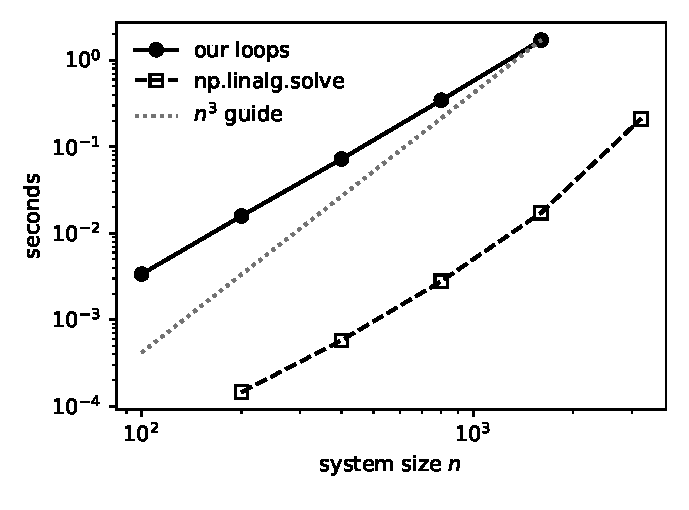
\includegraphics[width=0.75\linewidth]{figures/ch01_cost.pdf}
\caption{Measured cost of elimination vs $n$ on log-log axes, regenerated by \texttt{code/ch01\_cost\_figure.py}. Notice both curves trending toward the dotted $n^3$ guide: the algorithms differ only in their constant, not their shape. A slope of 3 on these axes is what ``cubic'' looks like.}
\label{fig:cost}
\end{figure}

\paragraph{The stability problem.} The count says nothing about whether the answer is \emph{right}. Floating-point arithmetic rounds every operation, and elimination can amplify rounding catastrophically when a pivot is tiny. Consider
\[
  \begin{bmatrix} 10^{-20} & 1\\ 1 & 1\end{bmatrix}\begin{bmatrix} x\\ y\end{bmatrix}=\begin{bmatrix} 1\\ 2\end{bmatrix},
  \qquad\text{true answer } x\approx1,\ y\approx1.
\]
Eliminating without a swap uses multiplier $10^{20}$: $R_2-10^{20}R_1$ gives $(1-10^{20})y=2-10^{20}$. In double precision $1-10^{20}=-10^{20}$, so $y=1$ exactly — and then the first equation reports $x=(1-y)/10^{-20}=0$. Plausible-looking output, confidently wrong. Swap the rows first and both multipliers stay below 1, giving $x\approx1$, $y\approx1$.

\begin{figure}[htbp]
\centering
% Figure 1.4: a tiny pivot without a swap produces a confidently wrong answer.
\begin{tikzpicture}[box/.style={draw,rounded corners=1pt,inner sep=4pt,align=center,font=\small},
  >=stealth]
\node[box,fill=amberbg] (p) {pivot $10^{-20}$\\[-2pt]\scriptsize tiny};
\node[box,fill=amberbg,right=1.1em of p] (m) {multiplier $10^{20}$\\[-2pt]\scriptsize huge};
\node[box,fill=amberbg,right=1.1em of m] (c) {$y\gets 1$\\[-2pt]\scriptsize plausible};
\node[box,fill=amberbg,right=1.1em of c] (w) {$x\gets(1-y)/10^{-20}=0$\\[-2pt]\scriptsize wrong: true $x\approx1$};
\draw[->,thick,amber] (p) -- (m);\draw[->,thick,amber] (m) -- (c);\draw[->,thick,amber] (c) -- (w);
\node[box,fill=goodbg,below=1.4em of m] (fix) {swap rows first: pivot $1$, multipliers $\le1$};
\draw[->,thick,good] (p.south) |- (fix.west);
\draw[->,thick,good] (fix.east) -| (w.south);
\end{tikzpicture}

\caption{How a tiny pivot destroys an answer, and the one-line fix. Notice the failure is silent — every intermediate number looks reasonable. This is why production solvers never take the diagonal entry as pivot blindly.}
\label{fig:pivfail}
\end{figure}

The fix is \emph{partial pivoting}\index{partial pivoting}: at each column, swap the largest-magnitude available entry into the pivot position. This keeps every multiplier $|\ell_{ik}|\le1$, which bounds how much rounding can grow (the \emph{growth factor}\index{growth factor} stays small for essentially all real problems). It costs a comparison per row — negligible against $n^3$ — and it is why \texttt{np.linalg.solve} computes $PA=LU$ with pivoting rather than the naive $LU$ of section~\ref{sec:lu}.

\begin{exercise}[hard]
Run the $10^{-20}$ system in Python three ways: no pivoting, with the row swap, and \texttt{np.linalg.solve}. Report the three $x$-values. Then replace $10^{-20}$ by $10^{-8}$: at what pivot size does the no-swap answer recover, and why?
\end{exercise}

\section{Hand derivation}\label{sec:handderiv}

Close the interpreter. Prove theorem~\ref{thm:affinesol} from scratch: the solution set of $A\mathbf{x}=\mathbf{b}$ is a particular solution plus the whole null space.
\begin{enumerate}
  \item Show that the set $S=\{\mathbf{x}_p+\mathbf{x}_h:\mathbf{x}_h\in N(A)\}$ contains only solutions (the $S\subseteq\{\text{solutions}\}$ direction).
  \item Show that every solution lies in $S$.
  \item Apply it: for example~\ref{ex:singular}, verify directly that the difference of any two solutions you can name is a multiple of $(1,-1,1)^{T}$.
  \item Conclude the count: if $A$ is $m\times n$ of rank $r$, the solution set (when non-empty) is a flat of dimension $n-r$. Why does that make ``exactly two solutions'' impossible?
\end{enumerate}

\section{Common mistakes}\label{sec:mistakes}

\begin{tripwire}[Sign errors in elimination bookkeeping]
Subtracting a multiple of a row the wrong way — $R_3+R_1$ when you meant $R_3-R_1$ — is the single most common error by hand. Defence: after each step, \emph{recheck one untouched entry} and recompute one new zero explicitly. In code, always compare against \texttt{np.linalg.solve} before trusting a hand-rolled elimination.
\end{tripwire}
\begin{tripwire}[Assuming every square system has a unique solution]
Square says nothing: $2\times2$ can be inconsistent or underdetermined. The pivot structure of the echelon form — not the shape of $A$ — decides between the four cases of figure~\ref{fig:solgeom}.
\end{tripwire}
\begin{tripwire}[Confusing pivot and free variables]
A variable is free iff its \emph{column} lacks a pivot — the test is on the matrix, not on which variables ``look'' free. Mislabeling here corrupts the whole parametrized solution in examples like~\ref{ex:singular}.
\end{tripwire}
\begin{tripwire}[Solving without pivoting and trusting garbage]
A zero or tiny pivot does not mean ``no solution'' — it means ``swap a row''. And a solver that ran to completion still may have produced a wrong $\mathbf{x}$; the residual $\|A\mathbf{x}-\mathbf{b}\|$ is cheap, so compute it.
\end{tripwire}

\section{Summary}\label{sec:ch1summary}

\begin{center}
\small
\begin{tabularx}{\linewidth}{@{}lY Y@{}}
\toprule
\tablehead \thead{Concept} & \thead{Statement} & \thead{Where used next} \\
\midrule
Two pictures & $A\mathbf{x}=\mathbf{b}$ = intersecting hyperplanes (rows) = combination of columns & drives the vector-spaces chapter \\
Row operations & add multiple, scale, swap — all preserve the solution set & everywhere \\
Echelon form & stair-step zeros; pivots first-nonzero in row & definition~\ref{def:pivot} \\
Rank $r$ & number of pivots & vector-spaces chapter \\
Solution count & $0=c$ row: none; $r=n$: one; $r<n$: $\infty$ (dim $n-r$) & figure~\ref{fig:solgeom} \\
Solution shape & $\mathbf{x}_p + N(A)$ & theorem~\ref{thm:affinesol}; least squares \\
$PA=LU$ & multipliers into $L$; swaps into $P$; $U$ = echelon form & every solve later in book \\
Cost & $\sim n^3/3$ multiply-adds to factor; $O(n^2)$ per new $\mathbf{b}$ & optimisation chapters \\
Partial pivoting & largest $|a_{ik}|$ into pivot; keeps multipliers $\le1$ & all numerical work \\
\bottomrule
\end{tabularx}
\end{center}

\begin{wins}
You can now solve any small linear system by hand and read off the shape of its solution set without solving at all — the skill every later chapter assumes.
\end{wins}

\chapternotes{%
The structure follows MIT 18.06SC Unit I (\emph{Ax = b and the four subspaces}) \cite{ocw1806sc}: row/column pictures, elimination, $LU$, then the geometry of solution sets. The interactive Immersive Linear Algebra chapter on Gaussian elimination \cite{ila} is a good second pass for the geometry. VMLS chapter 8 \cite{vmls} treats the same material with a data-first slant and is the source of the exercise style used here. MML \S2.3 \cite{mml} covers elimination in the compact ``for ML'' register this book aims at. The pivoting example of section~\ref{sec:cost} is the standard one from Strang's textbook treatment \cite{strangILA}. Timing methodology is best-of-several-repeats after a warm-up call. For the competitive-programming reader this book is aimed at, Sannemo's \emph{Principles of Algorithmic Problem Solving} \cite{sannemo2025} is the sibling text --- its systems material overlaps this chapter's.}

\begin{rulebox}[{Watch instead}]
The first two lectures of MIT's 18.06 match this chapter's first half
almost section for section:
\begin{enumerate}
\item \emph{The Geometry of Linear Equations} --- MIT OpenCourseWare,
18.06 Lecture 1, 39:49,
\url{https://youtu.be/J7DzL2_Na80} --- the row and column pictures of
\S\ref{sec:rowcol} (accessed 2026-10-11).
\item \emph{Elimination with Matrices} --- MIT OpenCourseWare, 18.06
Lecture 2, 47:41, \url{https://youtu.be/QVKj3LADCnA} --- the
elimination-to-echelon mechanics of \S\ref{sec:elim}--\S\ref{sec:lu}
(accessed 2026-10-11).
\end{enumerate}
\end{rulebox}

\section*{Further reading}
\addcontentsline{toc}{section}{Further reading}

\begin{itemize}
\item G.~Strang, \emph{Introduction to Linear Algebra}, 6th ed., chs.~1--2
(textbook level) --- the canonical treatment of row/column pictures and
elimination this chapter follows. Companion to the lectures above.
\item MIT OpenCourseWare, \emph{18.06SC Linear Algebra, Fall 2011},
Unit I (self-study level) --- worked recitations on the same material.
Free at OCW (course ``18.06SC'', Unit I page), at
\url{https://ocw.mit.edu}. Verified 2026-10-11.
\item Str\"om, \AA str\"om, and Akenine-M\"oller, \emph{Immersive Linear
Algebra} (interactive level) --- free at \url{https://immersivemath.com},
chapter ``Gaussian elimination'' --- a second, visual pass at the
solution-set geometry. Verified 2026-10-11.
\item S.~Boyd and L.~Vandenberghe, \emph{Introduction to Applied Linear
Algebra} (VMLS), ch.~8 (free PDF),
\url{https://web.stanford.edu/~boyd/vmls/vmls.pdf} --- the data-first
version of our exercise style. Verified 2026-10-11.
\item Margalit and Rabinoff, \emph{Interactive Linear Algebra} (Georgia
Tech), ``Systems of Linear Equations'' --- free at
\url{https://textbooks.math.gatech.edu/ila/} --- hyperlinked
remediation for any step you found fast here. Verified 2026-10-11.
\item J.~Hefferon, \emph{Linear Algebra} (free textbook) --- rigorous
alternative take, with many more proofs than we give.\newline
\url{https://hefferon.net/linearalgebra/index.html}
Verified 2026-10-11.
\end{itemize}

\section*{Additional exercises}
\addcontentsline{toc}{section}{Additional exercises}

\begin{exercise}[easy]
Solve by elimination: $x+y=7$, $2x-y=2$. Sketch the row picture and the column picture.
\end{exercise}
\begin{exercise}[easy]
Write down the augmented matrix of $x_1-2x_2=1$, $3x_1+x_2=9$, $-x_1+x_2=0$, eliminate it, and state which of the four cases of figure~\ref{fig:solgeom} this is.
\end{exercise}
\begin{exercise}[easy]
How many pivots does $\begin{bmatrix} 1 & 2 & 3\\ 0 & 4 & 5\\ 0 & 0 & 6\end{bmatrix}$ have? What is its rank? How many free variables does $A\mathbf{x}=\mathbf{b}$ have?
\end{exercise}
\begin{exercise}[easy]
Is $(1,1,0)^{T}$ in the null space of $A=\begin{bmatrix} 1 & -1 & 2\\ 0 & 1 & 1\end{bmatrix}$? Is $(2,2,-1)^{T}$?
\end{exercise}
\begin{exercise}[medium]
Find all solutions: $x+2y-z=3$, $2x+4y-2z=6$, $x+y+z=3$. Write the answer as $\mathbf{x}_p+t\mathbf{x}_h$.
\end{exercise}
\begin{exercise}[medium]
Give a $3\times3$ example of each: (a) unique solution; (b) inconsistent; (c) a line of solutions; (d) a plane of solutions. Verify each by elimination.
\end{exercise}
\begin{exercise}[medium]
Factor $A=\begin{bmatrix} 0 & 2 & 1\\ 1 & 1 & 0\\ 2 & 0 & 3\end{bmatrix}$ as $PA=LU$, writing $P$, $L$, $U$ explicitly.
\end{exercise}
\begin{exercise}[medium]
Show that if $A=LU$ with $L$ unit lower triangular and $U$ invertible upper triangular, then solving $A\mathbf{x}=\mathbf{b}$ costs $O(n^2)$ once $L,U$ are known. Count the multiply-adds of both triangular solves exactly.
\end{exercise}
\begin{exercise}[medium]
Prove that the set of solutions of $A\mathbf{x}=\mathbf{0}$ is closed under addition and scalar multiplication (so $N(A)$ is a subspace). Where does the proof fail for $A\mathbf{x}=\mathbf{b}$, $\mathbf{b}\neq\mathbf{0}$?
\end{exercise}
\begin{exercise}[hard]
Implement Gaussian elimination with \emph{partial pivoting} in Python: at column $k$, swap the row with largest $|a_{ik}|$ (among $i\ge k$) into position before eliminating. Test on the $10^{-20}$ example of section~\ref{sec:cost} and on 50 random $20\times20$ systems against \texttt{np.linalg.solve}. File: \texttt{code/ch01\_partial\_pivoting.py}.
\end{exercise}
\begin{exercise}[hard]
A \emph{tridiagonal} matrix has nonzeros only on the diagonal and its two neighbours. Show that elimination on an $n\times n$ tridiagonal matrix costs $O(n)$, not $O(n^3)$, by counting operations — then implement and time it for $n$ up to $10^6$.
\end{exercise}
\begin{exercise}[hard]
Prove that $A=LU$ (no swaps needed) exists iff every leading $k\times k$ submatrix of $A$ is invertible. (Hint: what makes each pivot nonzero?) This is why pivoting is sometimes a mathematical necessity, not just a numerical one.
\end{exercise}
\begin{exercise}[medium]
Balance butane combustion, $a\,\mathrm{C}_4\mathrm{H}_{10} + b\,\mathrm{O}_2 \to c\,\mathrm{CO}_2 + d\,\mathrm{H}_2\mathrm{O}$, by writing the three atom equations, finding the free-variable family, and taking the smallest whole numbers.
\end{exercise}
\begin{exercise}[medium]
Using the $LU$ of example~\ref{ex:twob}, solve $A\mathbf{x}=(2,5,4)^{T}$ without re-factoring --- then verify by multiplying $A$ times your answer.
\end{exercise}
\begin{exercise}[hard]
Show a homogeneous system $A\mathbf{x}=\mathbf{0}$ is never inconsistent. Deduce that a chemical-balance system always has infinitely many solutions whenever there are more unknown coefficients than elements, and explain why ``take the smallest positive integers'' is a convention, not a theorem.
\end{exercise}

\chapter{Matrices and matrix algebra}\label{ch:matrices}

Chapter 1 used a matrix as a box of coefficients feeding an algorithm. This chapter treats the matrix as an object in its own right — something you can multiply, transpose, invert and factor — and builds the small algebra that every later chapter uses without comment. After it you will be able to (a) read $A\mathbf{x}$ as a weighted combination of $A$'s columns; (b) read $AB$ both as composition of two actions and as a grid of inner products; (c) decide when $A^{-1}$ exists and compute it by Gauss--Jordan; and (d) recognize the four special matrix shapes that make algebra cheap: diagonal, triangular, permutation, block.

\section{A matrix is a box of coefficients --- and a recipe}\label{sec:matdef}

An $m\times n$ \emph{matrix}\index{matrix} $A$ is a rectangular array of numbers with $m$ rows and $n$ columns; we write $a_{ij}$ or $A_{ij}$ for the entry in row $i$, column $j$. That is the storage view. The operational view — the one worth tattooing — is that $A$ is a \emph{recipe}\index{matrix!as transformation}: feed it a vector $\mathbf{x}\in\mathbb{R}^n$ and it produces a vector $A\mathbf{x}\in\mathbb{R}^m$. A $3\times3$ matrix is a machine $\mathbb{R}^3\to\mathbb{R}^3$; a $2\times3$ matrix maps $\mathbb{R}^3\to\mathbb{R}^2$. Nothing about a matrix is mysterious once you hold both views: the box \emph{is} the recipe, written out entry by entry.

Two special members of the family show up constantly. The \emph{zero matrix}\index{zero matrix} $0$ sends everything to $\mathbf{0}$. The \emph{identity matrix}\index{identity matrix} $I_n$ — ones on the diagonal, zeros elsewhere — is the recipe ``change nothing'': $I_n\mathbf{x}=\mathbf{x}$. And matrices of the same shape add entrywise: $(A+B)_{ij}=a_{ij}+b_{ij}$, which is exactly ``do both recipes and add the results''; likewise $cA$ scales every entry. So the set of $m\times n$ matrices is itself a vector space — a fact the vector-spaces chapter cashes in.

\section{\texorpdfstring{$A\mathbf{x}$}{Ax} as a column combination}\label{sec:axcol}

Chapter 1 introduced the column picture for solving; here it becomes the definition. The product $A\mathbf{x}$ is the combination of $A$'s \emph{columns} weighted by the entries of $\mathbf{x}$:
\[
  A\mathbf{x} = x_1\mathbf{a}_1 + x_2\mathbf{a}_2 + \cdots + x_n\mathbf{a}_n,
  \qquad \mathbf{a}_j = \text{column $j$ of } A.
\]

\begin{example}\label{ex:axcol}
Compute $A\mathbf{x}$ for
\(
  A=\begin{bmatrix} 1 & 0 & 2\\ 2 & 1 & 0\\ 0 & 1 & 1\end{bmatrix},
  \ \mathbf{x}=(3,-1,2)^{T}
\).
\textbf{Strategy.} Read $A\mathbf{x}$ column-wise: take $3$ of column 1, subtract one of column 2, add two of column 3. Then sanity-check one entry the row way.
\begin{solution}
$3\mathbf{a}_1 - 1\mathbf{a}_2 + 2\mathbf{a}_3
 = 3(1,2,0)^{T} - (0,1,1)^{T} + 2(2,0,1)^{T}
 = (7,5,1)^{T}$.
Row check: row 1 gives $1\cdot3+0\cdot(-1)+2\cdot2=7$; row 2 gives $6-1+0=5$; row 3 gives $0-1+2=1$. \checkmark
\end{solution}
\end{example}

\begin{figure}[htbp]
\centering
% Figure: Ax as a weighted combination of the columns of A.
\begin{tikzpicture}[scale=0.9,>=stealth]
  \draw[->,gray] (-2.2,0) -- (4.4,0) node[below left] {\small $x$};
  \draw[->,gray] (0,-0.8) -- (0,4.8) node[below left] {\small $y$};
  % columns of A
  \draw[->,thick] (0,0) -- (2,1) node[midway,below right=-1pt] {\small $\mathbf a_1$};
  \draw[->,thick,dashed] (0,0) -- (-1,1.5) node[midway,above left=-2pt] {\small $\mathbf a_2$};
  % weighted copies, chained
  \draw[->,thick,accent] (0,0) -- (4,2) node[midway,sloped,below] {\small $2\mathbf a_1$};
  \draw[->,thick,dashed,accent] (4,2) -- (2.5,4.25) node[midway,sloped,above] {\small $+\,1.5\,\mathbf a_2$};
  \filldraw[accent] (2.5,4.25) circle (1.8pt) node[above=1pt] {\small $A\mathbf x$};
  \draw[dotted,gray] (2,1) -- (4,2);
\end{tikzpicture}

\caption{$A\mathbf{x}$ as a weighted column combination. Notice the recipe nature of the picture: the columns $\mathbf a_1,\mathbf a_2$ are fixed by $A$; the weights come from $\mathbf x$; the output is where the chain ends. Change $\mathbf x$ and the endpoint moves — that motion \emph{is} the matrix acting.}
\label{fig:axcol}
\end{figure}

Two consequences fall out immediately and are worth memorizing rather than re-deriving. First, $A\mathbf{e}_j=\mathbf{a}_j$: multiplying by the $j$-th \emph{standard basis vector}\index{standard basis} $\mathbf{e}_j$ (1 in position $j$, 0 elsewhere) picks out column $j$ — so you can probe a matrix column by column. Second, $A\mathbf{x}=\mathbf{0}$ has a nontrivial solution exactly when the columns of $A$ are \emph{dependent}\index{linear dependence} (some column is a combination of the others). That single sentence is the seed of rank, null space, and invertibility all at once.

\begin{exercise}[easy]
Let $A=\begin{bmatrix} 2 & -1\\ 0 & 3\end{bmatrix}$, $\mathbf{x}=(4,1)^{T}$. Compute $A\mathbf{x}$ by the column rule, then verify entry 2 by the row rule. Then find a nonzero $\mathbf{x}$ with $A\mathbf{x}=(2,-1)^{T}$ — reading $A\mathbf{x}$ as a column combination, which column is being singled out?
\end{exercise}

\section{Matrix multiplication as composition}\label{sec:matmul}

If $B$ is a recipe and $A$ is a recipe, the obvious thing to build is ``do $B$ first, then $A$'' — the \emph{composition}\index{composition} $A\circ B$. Matrix multiplication is exactly that, packaged as one matrix:
\[
  (AB)\mathbf{x} = A(B\mathbf{x}), \qquad\text{for every }\mathbf{x}.
\]
Working out what entry of $AB$ must be to make this true gives the familiar rule: if $A$ is $m\times k$ and $B$ is $k\times n$,
\[
  (AB)_{ij} = \sum_{l=1}^{k} a_{il}\,b_{lj} = (\text{row $i$ of }A)\cdot(\text{column $j$ of }B).
\]
The product exists only when the inner dimensions match — columns of $A$ = rows of $B$ — and the result is $m\times n$. Figure~\ref{fig:abgrid} is the picture to hold: entry $(i,j)$ lives where row $i$ of $A$ meets column $j$ of $B$.

\begin{figure}[htbp]
\centering
% Figure: (AB)_{ij} is the inner product of row i of A with column j of B.
\begin{tikzpicture}[scale=0.52,every node/.style={inner sep=0pt,minimum size=0.52cm}]
  % --- A: 3x2, row 2 highlighted ---
  \foreach \r/\c/\v in {0/0/1,0/1/2,1/0/0,1/1/1,2/0/3,2/1/0}
    \node[draw] (A-\r-\c) at (\c,-\r) {$\v$};
  \foreach \c in {0,1} \node[draw,fill=accentsoft,minimum width=0.52cm] at (\c,-1) {};
  \node[draw,fill=accentsoft] (A-1-0) at (0,-1) {$0$};
  \node[draw,fill=accentsoft] (A-1-1) at (1,-1) {$1$};
  \node[left=3pt of A-1-0] {\scriptsize row $i$};
  \node[below=4pt] at (0.5,-2) {\small $A$};
  % --- B: 2x3, col 3 highlighted ---
  \begin{scope}[xshift=3.2cm]
    \foreach \r/\c/\v in {0/0/2,0/1/1,0/2/0,1/0/1,1/1/3,1/2/1}
      \node[draw] (B-\r-\c) at (\c,-\r) {$\v$};
    \node[draw,fill=accentsoft] (B-0-2) at (2,0) {$0$};
    \node[draw,fill=accentsoft] (B-1-2) at (2,-1) {$1$};
    \node[above=3pt of B-0-2] {\scriptsize col $j$};
    \node[below=4pt] at (1,-2) {\small $B$};
  \end{scope}
  % --- equals ---
  \node at (7.0,-0.5) {\large $=$};
  % --- C: 3x3 with (2,3) highlighted ---
  \begin{scope}[xshift=7.7cm]
    \foreach \r in {0,1,2} \foreach \c in {0,1,2}
      \node[draw] (C-\r-\c) at (\c,-\r) {};
    \node[draw,fill=accentsoft] (C-1-2) at (2,-1) {\scriptsize $\cdot$};
    \node[right=2pt of C-1-2] {\scriptsize $c_{ij}=\mathbf a_{i,:}\!\cdot\!\mathbf b_{:,j}$};
    \node[below=4pt] at (1,-2) {\small $AB$};
  \end{scope}
\end{tikzpicture}

\caption{$AB$ as a grid of inner products. Notice the highlighted cell: its value is row $i$ of $A$ dotted with column $j$ of $B$, and nothing else in either matrix touches it. Each of the $mn$ cells is an independent dot product — which is also why matrix multiplication parallelizes so well.}
\label{fig:abgrid}
\end{figure}

The algebra that follows is best learned by contrast with numbers:

\begin{itemize}
  \item \emph{Associative}\index{associativity}: $A(BC)=(AB)C$, always — because both sides mean ``$C$, then $B$, then $A$'' and composition is unambiguous. (You will prove this properly in the hand derivation.)
  \item \emph{Distributive}: $A(B+C)=AB+AC$ and $(A+B)C=AC+BC$.
  \item \emph{Not commutative}\index{commutativity!fails}: $AB\neq BA$ in general. Order matters because the recipes do different things in different orders — and because often only one of the two products is even defined.
\end{itemize}

\begin{lstlisting}[language=Python,caption={Naive triple-loop \texttt{matmul} against \texttt{np.matmul}: correct, and painfully slow. File: \texttt{code/ch02\_matmul\_triple.py}.},label={lst:matmul}]
import time
import numpy as np

def matmul(A, B):
    n, k, m = A.shape[0], B.shape[0], B.shape[1]
    C = np.zeros((n, m))
    for i in range(n):
        for j in range(m):
            for l in range(k):
                C[i, j] += A[i, l] * B[l, j]
    return C

rng = np.random.default_rng(1)
np.seterr(all="ignore")      # Accelerate BLAS prints spurious fp warnings
np.matmul(np.eye(4), np.eye(4))   # warm-up

print(f"{'n':>5} {'ours (s)':>10} {'np (s)':>10} {'agree?':>8}")
for n in [128, 256]:
    A, B = rng.standard_normal((n, n)), rng.standard_normal((n, n))
    t0 = time.perf_counter(); C_ours = matmul(A, B); t1 = time.perf_counter()
    t2 = time.perf_counter(); C_np = np.matmul(A, B); t3 = time.perf_counter()
    print(f"{n:>5} {t1-t0:>10.4f} {t3-t2:>10.4f} {str(np.allclose(C_ours, C_np)):>8}")
for n in [512, 1024]:
    A, B = rng.standard_normal((n, n)), rng.standard_normal((n, n))
    t2 = time.perf_counter(); np.matmul(A, B); t3 = time.perf_counter()
    print(f"{n:>5} {'--':>10} {t3-t2:>10.4f} {'--':>8}")
\end{lstlisting}

\begin{lstlisting}[caption={Output of listing~\ref{lst:matmul}. Our loop agrees exactly with the library — the rule is the same; doubling $n$ multiplies our time by $\sim8$ ($2n^3$ multiply-adds), while LAPACK stays four orders of magnitude faster by blocking for cache.}]
    n   ours (s)     np (s)   agree?
  128     0.4196     0.0001     True
  256     3.3752     0.0002     True
  512         --     0.0007       --
 1024         --     0.0062       --
\end{lstlisting}

\begin{exercise}[easy]
For $A=\begin{bmatrix}1&2\\0&1\end{bmatrix}$ and $B=\begin{bmatrix}1&0\\1&1\end{bmatrix}$, compute $AB$ and $BA$ by hand. Are they equal? Then explain in one sentence what each does to the vector $\mathbf{e}_1$.
\end{exercise}

\begin{example}\label{ex:adjacency}
The small graph of figure~\ref{fig:graph} has edges
$1{-}2$, $1{-}3$, $2{-}3$, $3{-}4$. How many two-step walks go from
vertex $1$ to vertex $3$?
\par\smallskip
\textbf{Strategy.} Write the adjacency matrix $A$ with $a_{ij}=1$ when
$i{-}j$ is an edge. Then $(A^2)_{ij}=\sum_k a_{ik}a_{kj}$ counts walks
$i\to k\to j$ --- a matrix product that is literally a path counter.
\begin{solution}
$A=\begin{bmatrix}0&1&1&0\\1&0&1&0\\1&1&0&1\\0&0&1&0\end{bmatrix}$,
and
$(A^2)_{13}=a_{11}a_{13}+a_{12}a_{23}+a_{13}a_{33}+a_{14}a_{43}
 =0+1\cdot1+0+0=1$. The single two-step walk is $1\to2\to3$ ---
$1\to3\to3$ is not a walk because there is no loop edge $3{-}3$.
The same square gives $(A^2)_{33}=3$ (three two-step loops back to 3).
\checkmark
\end{solution}
\end{example}

\begin{figure}[htbp]\centering
% Figure 2.5: the adjacency matrix and its square.
% (A^2)_ij counts two-step walks i -> * -> j.
\begin{tikzpicture}[scale=0.95,>=stealth,
  vtx/.style={circle,draw,thick,inner sep=1.6pt,font=\small}]
  % left: the graph
  \begin{scope}
    \node[vtx] (n1) at (0,1.6) {1};
    \node[vtx] (n2) at (2.2,1.6) {2};
    \node[vtx] (n3) at (0,0) {3};
    \node[vtx] (n4) at (2.2,0) {4};
    \draw[thick] (n1) -- (n2);
    \draw[thick] (n2) -- (n3);
    \draw[thick] (n3) -- (n4);
    \draw[thick] (n1) -- (n3);
    \node at (1.1,-0.8) {\small walks $1\to3$ in two steps:};
    \node at (1.1,-1.3) {\small $1\to2\to3$ and $1\to3\to\cdots$?};
  \end{scope}
  % right: A and A^2
  \begin{scope}[xshift=6.2cm,yshift=0.4cm]
    \node[font=\small] at (1.3,2.3) {$A=\begin{bmatrix}
      0&1&1&0\\1&0&1&0\\1&1&0&1\\0&0&1&0\end{bmatrix}$};
    \node[font=\small] at (5.2,2.3) {$A^2=\begin{bmatrix}
      2&1&1&1\\1&2&1&1\\1&1&3&0\\1&1&0&1\end{bmatrix}$};
    \node[font=\small,align=center] at (3.2,0.4) {$(A^2)_{13}=1$: exactly one two-step\\ walk from 1 to 3, namely $1\to2\to3$};
  \end{scope}
\end{tikzpicture}

\caption{The adjacency matrix squared counts two-step walks. Notice
why matrix multiplication is the right tool: entry $(i,j)$ of $A^2$
sums over \emph{every possible middle stop} $k$ --- the dot-product
grid of figure~\ref{fig:abgrid} is a walk counter.}
\label{fig:graph}
\end{figure}

\section{Transpose, inverses, and when they exist}\label{sec:transposeinv}

The \emph{transpose}\index{transpose} $A^{T}$ flips a matrix across its diagonal: $(A^{T})_{ij}=a_{ji}$ — rows become columns. Two rules carry the whole algebra of the transpose:
\[
  (A^{T})^{T}=A, \qquad (AB)^{T}=B^{T}A^{T}.
\]
The second is the \emph{reverse-order} rule and it surprises everyone once. Why reversed? Because $(AB)\mathbf{x}=A(B\mathbf{x})$, and an inner product reads symmetrically: row $i$ of $AB$ dotted with $\mathbf{x}$ equals column $i$ of $B^{T}A^{T}$ dotted with $\mathbf{x}$ — the next example makes it concrete. A \emph{symmetric}\index{symmetric matrix} matrix satisfies $A^{T}=A$; they own the spectral theorem later, and you build one for free whenever you form $A^{T}A$.

\begin{example}\label{ex:transp}
Verify $(AB)^{T}=B^{T}A^{T}$ on paper for $A=\begin{bmatrix}1&2\\3&4\end{bmatrix}$, $B=\begin{bmatrix}0&1\\1&0\end{bmatrix}$, then prove it in general.
\textbf{Strategy.} Compute both sides on the $2\times2$ case first — one matrix each, ten seconds — and only then do the index bookkeeping for the proof. The check is not the proof; it is what keeps the proof honest.
\begin{solution}
$AB=\begin{bmatrix}2&1\\4&3\end{bmatrix}$, so $(AB)^{T}=\begin{bmatrix}2&4\\1&3\end{bmatrix}$. And $B^{T}A^{T}=\begin{bmatrix}0&1\\1&0\end{bmatrix}\begin{bmatrix}1&3\\2&4\end{bmatrix}=\begin{bmatrix}2&4\\1&3\end{bmatrix}$. Equal. \checkmark
\emph{Proof.} The $(i,j)$ entry of $(AB)^{T}$ is the $(j,i)$ entry of $AB$: $\sum_l a_{jl}b_{li}$. The $(i,j)$ entry of $B^{T}A^{T}$ is $\sum_l (B^{T})_{il}(A^{T})_{lj}=\sum_l b_{li}a_{jl}$ — the same sum, terms commuted. $\square$
\end{solution}
\end{example}

Now the inverse. A square matrix $A$ is \emph{invertible}\index{inverse}\index{invertible} when a matrix $A^{-1}$ exists with
\[
  A^{-1}A = I = AA^{-1}.
\]
Invertible means exactly: the recipe can be undone — $A$ sends distinct inputs to distinct outputs and hits everything in range. Chapter-1 language translates that into a test you already own: \emph{$A$ is invertible iff elimination produces $n$ pivots} (iff the only solution of $A\mathbf{x}=\mathbf{0}$ is $\mathbf{x}=\mathbf{0}$, iff the columns are independent). To actually compute $A^{-1}$, run elimination on the $2n$-column matrix $[\,A\mid I\,]$ and continue past echelon form until the left half is $I$; the right half is then $A^{-1}$. This is \emph{Gauss--Jordan elimination}\index{Gauss--Jordan}.

\begin{figure}[htbp]
\centering
% Figure: inverse as the map that undoes A; and AB undone one factor at a time.
\begin{tikzpicture}[>=stealth,node distance=2.1cm,every node/.style={align=center}]
  \node (x) {$\mathbf x$};
  \node (bx) [right=of x] {$B\mathbf x$};
  \node (abx) [right=of bx] {$AB\mathbf x$};
  \draw[->,thick] (x) -- (bx) node[midway,above] {\small $B$};
  \draw[->,thick] (bx) -- (abx) node[midway,above] {\small $A$};
  \draw[->,thick,accent] (abx.south) to[out=-30,in=-150] node[midway,below] {\small $A^{-1}$} (bx.south);
  \draw[->,thick,accent] (bx.south) to[out=-30,in=-150] node[midway,below] {\small $B^{-1}$} (x.south);
  \node[below=1.15cm of bx] (lbl) {\small undo $AB$ by undoing $A$ \emph{then} $B$:\\[1pt]\small$(AB)^{-1}=B^{-1}A^{-1}$};
\end{tikzpicture}

\caption{The inverse as undo, and why $(AB)^{-1}=B^{-1}A^{-1}$. Notice the order: to walk the chain back you must undo the \emph{last} step first. Same reason you take off shoes before socks.}
\label{fig:inverseundo}
\end{figure}

\begin{example}\label{ex:inverse}
Invert $A=\begin{bmatrix}1&2&0\\2&5&1\\0&1&3\end{bmatrix}$ by Gauss--Jordan.
\textbf{Strategy.} Augment $[\,A\mid I\,]$, eliminate down to echelon form exactly as in Chapter~1, then keep going: scale each pivot to 1 and clear \emph{upward} so the left half becomes $I$. Whatever happened to the right half is the answer.
\begin{solution}
\[
\left[\begin{array}{ccc|ccc}1&2&0&1&0&0\\2&5&1&0&1&0\\0&1&3&0&0&1\end{array}\right]
\to\left[\begin{array}{ccc|ccc}1&2&0&1&0&0\\0&1&1&-2&1&0\\0&0&2&2&-1&1\end{array}\right]
\to\left[\begin{array}{ccc|ccc}1&0&0&7&-3&1\\0&1&0&-3&3/2&-1/2\\0&0&1&1&-1/2&1/2\end{array}\right]
\]
($R_2-2R_1$, then $R_3-R_2$, then scale and clear upward.) So
\(
A^{-1}=\begin{bmatrix}7&-3&1\\-3&3/2&-1/2\\1&-1/2&1/2\end{bmatrix}
\), and the code below confirms $AA^{-1}=I$ exactly.
\end{solution}
\end{example}

\begin{lstlisting}[language=Python,caption={Gauss--Jordan inverse on example~\ref{ex:inverse}, verified against \texttt{np.linalg.inv}. File: \texttt{code/ch02\_gauss\_jordan\_inverse.py}.},label={lst:gj}]
import numpy as np

A = np.array([[1., 2., 0.], [2., 5., 1.], [0., 1., 3.]])
n = A.shape[0]
AI = np.column_stack([A, np.eye(n)])

for col in range(n):
    AI[col] = AI[col] / AI[col, col]        # normalize pivot row
    for row in range(n):
        if row != col:
            AI[row] -= AI[row, col] * AI[col]  # kill the column elsewhere

A_inv = AI[:, n:]
print("A_inv by Gauss-Jordan:")
print(A_inv)
print("np.linalg.inv agrees:", np.allclose(A_inv, np.linalg.inv(A)))
print("A @ A_inv:")
print(A @ A_inv)
\end{lstlisting}

\begin{lstlisting}[caption={Output of listing~\ref{lst:gj}. The hand computation and the library agree to the last digit; $AA^{-1}=I$ on the nose.}]
A_inv by Gauss-Jordan:
[[ 7.  -3.   1. ]
 [-3.   1.5 -0.5]
 [ 1.  -0.5  0.5]]
np.linalg.inv agrees: True
A @ A_inv:
[[1. 0. 0.]
 [0. 1. 0.]
 [0. 0. 1.]]
\end{lstlisting}

The practical rule deserves its own line, because violating it is a rite of passage everyone fails once: \textbf{never compute $A^{-1}$ to solve $A\mathbf{x}=\mathbf{b}$.} Chapter 1's $LU$ solve is faster, more stable, and gives the same answer. The inverse exists in this book as an algebraic object — for proofs, small closed forms, and understanding — not as a solver.

\begin{exercise}[medium]
Two claims, prove or disprove each: (a) if $A$ and $B$ are invertible, so is $AB$, and $(AB)^{-1}=B^{-1}A^{-1}$; (b) if $AB=I$ for square $A,B$, then also $BA=I$. (For (b), think of $A$'s columns: what does $AB=I$ say about them?)
\end{exercise}

\section{Special matrices: diagonal, triangular, permutation, block}\label{sec:special}

Four shapes recur so often that each gets a name and a shortcut; figure~\ref{fig:gallery} shows three of them acting on the plane plus the fourth in box form.

\begin{description}
\item[Diagonal\index{diagonal matrix}] $D=\mathrm{diag}(d_1,\dots,d_n)$: scales axis $i$ by $d_i$ and does nothing else. $D\mathbf{x}$ is entrywise scaling; $D_1D_2$ is diagonal again ($d_id_i'$); $D^{-1}=\mathrm{diag}(1/d_i)$ when no $d_i=0$. The cheapest matrix there is — eigenvalue theory later asks ``how close to diagonal can we make $A$?''
\item[Triangular\index{triangular matrix}] upper $U$ or lower $L$: the output of Chapter~1. Triangular systems solve by substitution in $O(n^2)$; products stay triangular; diagonal entries are the pivots (Chapter~6: the eigenvalues).
\item[Permutation\index{permutation matrix}] $P$: $I$ with rows reordered — one 1 per row and column. $P\mathbf{x}$ relabels coordinates; $P^{T}=P^{-1}$ undoes it. They are why `shuffle' and `reorder' are free in linear algebra.
\item[Block\index{block matrix}] $\begin{bmatrix}A_{11}&A_{12}\\A_{21}&A_{22}\end{bmatrix}$: matrices whose entries are matrices. The multiplication rule is unchanged — block row times block column, summed — provided every inner product is dimensionally legal. Proofs and parallel code both lean on this constantly.
\end{description}

\begin{figure}[htbp]
\centering
% Figure: what the special matrices do to the unit square, plus block form.
\begin{tikzpicture}[scale=0.62,>=stealth,sq/.style={thick,fill=accentsoft}]
  % (a) diagonal: axis scaling
  \begin{scope}
    \draw[->,gray] (-0.4,0) -- (2.7,0);\draw[->,gray] (0,-0.4) -- (0,1.9);
    \draw[sq] (0,0) -- (1,0) -- (1,1) -- (0,1) -- cycle;
    \draw[sq,fill=accent] (0,0) -- (2,0) -- (2,0.5) -- (0,0.5) -- cycle;
    \node at (1.15,-1.15) {\small (a) diag$(2,\tfrac12)$};
  \end{scope}
  % (b) permutation: swaps the axes
  \begin{scope}[xshift=3.9cm]
    \draw[->,gray] (-0.4,0) -- (2.7,0) node[below left] {\scriptsize$y$};
    \draw[->,gray] (0,-0.4) -- (0,1.9) node[below left] {\scriptsize$x$};
    \draw[sq] (0,0) -- (1,0) -- (1,1) -- (0,1) -- cycle;
    \draw[->,accent,thick] (1.45,0.4) to[out=30,in=-30] (0.4,1.45);
    \node at (1.15,-1.15) {\small (b) permutation};
  \end{scope}
  % (c) triangular (shear): tips the top over
  \begin{scope}[xshift=7.8cm]
    \draw[->,gray] (-0.4,0) -- (3.4,0);\draw[->,gray] (0,-0.4) -- (0,1.9);
    \draw[sq] (0,0) -- (1,0) -- (1,1) -- (0,1) -- cycle;
    \draw[sq,fill=accent] (0,0) -- (1,0) -- (2,1) -- (1,1) -- cycle;
    \node at (1.4,-1.15) {\small (c) $\begin{bsmallmatrix}1&1\\0&1\end{bsmallmatrix}$ (shear)};
  \end{scope}
  % (d) block: same rules, bigger boxes
  \begin{scope}[xshift=11.9cm,scale=0.55]
    \draw[thick] (0,0) rectangle (4,4);
    \draw[thick] (2,0) -- (2,4); \draw[thick] (0,2) -- (4,2);
    \node at (1,3) {$A_{11}$};\node at (3,3) {$A_{12}$};
    \node at (1,1) {$A_{21}$};\node at (3,1) {$A_{22}$};
    \node at (2,-1.15) {\small (d) block matrix};
  \end{scope}
\end{tikzpicture}

\caption{Three special matrices acting on the unit square, and the fourth in box form. Notice that diagonal only stretches axes, permutation only relabels them, and the shear (upper triangular) leaves the bottom edge alone — the special structures are exactly the restrictions that make their algebra cheap.}
\label{fig:gallery}
\end{figure}

\begin{lstlisting}[language=Python,caption={A permutation matrix is a reorder, and $P^{T}$ undoes it — the same trick a data loader uses when it shuffles sample order. File: \texttt{code/ch02\_permutation\_dataset.py}.},label={lst:perm}]
import numpy as np

# a tiny "dataset": each row tagged with its original index
X = np.array([[0., 10.], [1., 11.], [2., 12.], [3., 13.]])
sigma = [2, 0, 3, 1]              # new order of rows

n = len(sigma)
P = np.zeros((n, n))
P[np.arange(n), sigma] = 1        # row i of PX is row sigma[i] of X

print("P =\n", P)
print("P @ X =\n", P @ X)
print("X[sigma] =\n", X[sigma])
print("same thing:", np.allclose(P @ X, X[sigma]))
print("P.T @ P = I:", np.allclose(P.T @ P, np.eye(n)))
print("undo with P.T:", np.allclose(P.T @ (P @ X), X))
\end{lstlisting}

\begin{lstlisting}[caption={Output of listing~\ref{lst:perm}. $P@X$ is exactly fancy-indexing \texttt{X[sigma]}; $P^{T}P=I$ because a permutation never duplicates or drops a row.}]
P =
 [[0. 0. 1. 0.]
 [1. 0. 0. 0.]
 [0. 0. 0. 1.]
 [0. 1. 0. 0.]]
P @ X =
 [[ 2. 12.]
 [ 0. 10.]
 [ 3. 13.]
 [ 1. 11.]]
X[sigma] =
 [[ 2. 12.]
 [ 0. 10.]
 [ 3. 13.]
 [ 1. 11.]]
same thing: True
P.T @ P = I: True
undo with P.T: True
\end{lstlisting}

\begin{example}\label{ex:perm}
Shuffle a three-row dataset $A$ so that row 3 comes first, then rows 1
and 2 in order. Write the matrix that does it --- and check it really is
a \emph{permutation matrix}.
\par\smallskip
\textbf{Strategy.} A row shuffle is a left multiplication (row
operations live on the left). Build $P$ row by row: row $i$ of $PA$
should be the picked row of $A$ --- put a single $1$ in the right
column.
\begin{solution}
We want $(PA)_1=A_3$, $(PA)_2=A_1$, $(PA)_3=A_2$:
\[
  P=\begin{bmatrix}0&0&1\\1&0&0\\0&1&0\end{bmatrix},\qquad
  PA=\begin{bmatrix}a_{31}&a_{32}\\a_{11}&a_{12}\\a_{21}&a_{22}\end{bmatrix}.
\]
Each row of $P$ is a standard basis row $\mathbf{e}_j^{T}$, which
\emph{picks} row $j$ of $A$ (figure~\ref{fig:perm}). Every row shuffle
of a training set is exactly this: one left multiplication, no data
touched twice, invertible by $P^{T}$. \checkmark
\end{solution}
\end{example}

\begin{figure}[htbp]\centering
% Figure 2.6: a permutation matrix is a shuffle, nothing more.
% PA moves row i of A to the position the 1 in row i of P indicates.
\begin{tikzpicture}[scale=1.0,>=stealth,
  lbl/.style={font=\small}]
  \node[lbl] at (0,1.7) {$P=\begin{bmatrix}0&0&1\\1&0&0\\0&1&0\end{bmatrix}$};
  \node[lbl] at (3.4,1.7) {$A=\begin{bmatrix}a_{11}&a_{12}\\a_{21}&a_{22}\\a_{31}&a_{32}\end{bmatrix}$};
  \node[lbl] at (7.6,1.7) {$PA=\begin{bmatrix}a_{31}&a_{32}\\a_{11}&a_{12}\\a_{21}&a_{22}\end{bmatrix}$};
  % arrows: where each row of A lands
  \draw[->,thick,accent] (4.3,1.95) .. controls (5.4,2.5) .. (7.1,2.0);
  \draw[->,thick] (4.3,1.7) .. controls (5.2,1.5) .. (7.1,1.5);
  \draw[->,thick] (4.3,1.45) .. controls (5.2,0.9) .. (7.1,1.0);
  \node[lbl] at (5.5,2.7) {row 3 $\to$ top};
  \node[lbl,font=\footnotesize] at (3.4,0.5) {each row of $P$ is one $\mathbf{e}_j$:};
  \node[lbl,font=\footnotesize] at (3.4,0.05) {it \emph{picks} that row of $A$};
\end{tikzpicture}

\caption{A permutation matrix is a shuffle. Notice the mechanism: each
row of $P$ is one $\mathbf{e}_j^{T}$, and $\mathbf{e}_j^{T}A$ is row
$j$ of $A$ --- a product of picks.}
\label{fig:perm}
\end{figure}

\section{Hand derivation}\label{sec:handderiv2}

Two proofs, both short, both worth doing with the interpreter closed.
\begin{enumerate}
  \item Prove $(AB)^{-1}=B^{-1}A^{-1}$ directly from the definition: a matrix $X$ is \emph{the} inverse of $M$ iff $MX=I$ and $XM=I$. Compute $(B^{-1}A^{-1})(AB)$ and $(AB)(B^{-1}A^{-1})$ using associativity only — no entries allowed. Conclude uniqueness of the inverse: if $X$ and $Y$ both satisfy the definition for $A$, then $X=Y$ (multiply $AX=I$ by $Y$ on the left).
  \item Prove associativity $(AB)C=A(BC)$ via composition: define $f_B(\mathbf{x})=B\mathbf{x}$ and show both sides name the same function, $f_A\circ f_B\circ f_C$, applied to an arbitrary $\mathbf{x}$. This is the ``functions compose associatively'' argument — write it out fully, including the step where you use the definition $(MN)\mathbf{x}=M(N\mathbf{x})$.
\end{enumerate}

\section{Common mistakes}\label{sec:mistakes2}

\begin{tripwire}[Assuming $AB=BA$]
Matrix multiplication is not commutative, full stop. When a manipulation needs you to swap the order — expanding $(A+B)^2$, moving a term past another — write out both orders first and check which you actually have. $(A+B)^2=A^2+AB+BA+B^2$, and that middle pair usually cannot merge.
\end{tripwire}
\begin{tripwire}[Wrong order in $(AB)^{T}$]
The transpose of a product is the product of the transposes \emph{reversed}: $B^{T}A^{T}$, not $A^{T}B^{T}$. Same reversal for inverses. Mnemonic: to undo $AB$ you meet $B$ last, so $B$'s undo comes first.
\end{tripwire}
\begin{tripwire}[Dimension mismatches read as ``almost right'']
A $3\times2$ times a $3\times2$ is not ``nearly'' a product — it is undefined, and no reshaping the answer rescues it. Before every multiplication, name the shapes: $(m\times k)(k\times n)\to(m\times n)$. If the inner numbers disagree, stop.
\end{tripwire}
\begin{tripwire}[Believing every nonzero matrix is invertible]
$\begin{bmatrix}1&1\\1&1\end{bmatrix}$ is about as nonzero as matrices get, and it crushes the whole plane onto a line — no undo exists. Invertibility is about the columns being independent, which Chapter 1 already showed you how to test: $n$ pivots, or nothing.
\end{tripwire}

\section{Summary}\label{sec:ch2summary}

\begin{center}
\small
\begin{tabularx}{\linewidth}{@{}lY Y@{}}
\toprule
\tablehead \thead{Concept} & \thead{Statement} & \thead{Where used next} \\
\midrule
$A\mathbf{x}$ & column combination, weights from $\mathbf x$ & everything \\
$AB$ & composition; $(AB)_{ij}=$ row$_i\cdot$col$_j$; needs inner dims equal & every model \\
Associativity & $A(BC)=(AB)C$ via composition & proofs, chaining layers \\
$AB\neq BA$ & order is part of the meaning & commutator exercises \\
Transpose & $(A^T)_{ij}=a_{ji}$; $(AB)^T=B^TA^T$ & $A^TA$, symmetric ch. \\
Inverse & $AA^{-1}=I$; exists iff $n$ pivots; Gauss--Jordan on $[A|I]$ & least squares (formally) \\
$(AB)^{-1}$ & $B^{-1}A^{-1}$ — undo last step first & hand derivation \\
Never invert to solve & $LU$-solve is cheaper and stabler & all numerical work \\
Special shapes & diagonal (scale), triangular (substitute), permutation ($P^T=P^{-1}$), block (same rules) & rest of book \\
\bottomrule
\end{tabularx}
\end{center}

\begin{wins}
You can now multiply matrices both ways — as dot-product grids and as composed recipes — invert a small one by hand, and spot the four shapes that make later algebra cheap.
\end{wins}

\chapternotes{%
The composition-first treatment of matrix multiplication follows MIT 18.06SC Unit I \cite{ocw1806sc}; the column-combination mantra for $A\mathbf{x}$ is Strang's, restated. VMLS chapters 6 and 10 \cite{vmls} supply the data-first framing (the permutation-as-shuffle example is theirs in spirit) and the gallery treatment of special matrices. MML \S2.2 \cite{mml} is the compact reference for the same algebra. The Immersive Linear Algebra chapter on the matrix \cite{ila} has the interactive versions of figures~\ref{fig:axcol} and \ref{fig:abgrid}. The never-invert-to-solve rule is standard numerical practice \cite{strangILA}.}
\begin{rulebox}[{Watch instead}]
\begin{enumerate}
\item \emph{Matrix multiplication as composition} --- 3Blue1Brown,
Essence of Linear Algebra ch.~4, 10:03,
\url{https://youtu.be/XkY2DOUCWMU} --- the recipe-composition view of
\S\ref{sec:matmul} (accessed 2026-10-11).
\item \emph{Multiplication and Inverse Matrices} --- MIT OpenCourseWare,
18.06 Lecture 3, 46:49, \url{https://youtu.be/hMmXCdVym3A} --- the
five-product viewpoints plus Gauss--Jordan inversion of
\S\ref{sec:matmul}--\S\ref{sec:transposeinv} (accessed 2026-10-11).
\end{enumerate}
\end{rulebox}

\section*{Further reading}
\addcontentsline{toc}{section}{Further reading}

\begin{itemize}
\item G.~Strang, \emph{Introduction to Linear Algebra}, 6th ed., ch.~2
(textbook level) --- the matrix-multiplication and inverse material at
full length.
\item MIT OpenCourseWare, \emph{18.06SC Linear Algebra} --- the OCW
course pages behind the watch picks; worked recitations on products
and inverses. \newline
OCW (course ``18.06SC''), at \url{https://ocw.mit.edu}
Verified 2026-10-11.
\item S.~Boyd and L.~Vandenberghe, \emph{VMLS}, chs.~6, 10 (free PDF) ---
matrix algebra and inverses with data-first examples (the row-shuffle
view is theirs). \newline
\url{https://web.stanford.edu/~boyd/vmls/vmls.pdf}
Verified 2026-10-11.
\item Margalit and Rabinoff, \emph{Interactive Linear Algebra} (Georgia
Tech), ``Matrix Algebra'' --- the same algebra hyperlinked.\newline
\url{https://textbooks.math.gatech.edu/ila/}
Verified 2026-10-11.
\item M.~Deisenroth et al., \emph{Mathematics for Machine Learning},
\S2.2 (free PDF) --- the compact ML-register reference.\newline
\url{https://mml-book.github.io/book/mml-book.pdf}
Verified 2026-10-11.
\item Str\"om, \AA str\"om, and Akenine-M\"oller, \emph{Immersive Linear
Algebra}, chapter ``The matrix'' --- interactive versions of our
figures~\ref{fig:axcol} and \ref{fig:abgrid}. Free at
\url{https://immersivemath.com}. Verified 2026-10-11.
\end{itemize}

\section*{Additional exercises}
\addcontentsline{toc}{section}{Additional exercises}

\begin{exercise}[easy]
Let $A=\begin{bmatrix}1&-2\\3&0\end{bmatrix}$, $\mathbf{x}=(5,1)^{T}$, $\mathbf{y}=(0,4)^{T}$. Compute $A\mathbf{x}$, $A\mathbf{y}$, and $A(\mathbf{x}+\mathbf{y})$; confirm the third equals the sum of the first two. Which property of the recipe is that?
\end{exercise}
\begin{exercise}[easy]
For $A=\begin{bmatrix}2&1\\1&2\end{bmatrix}$, compute $A^{T}$, $AA^{T}$, and $A^{T}A$. Which two are equal here, and is that an accident?
\end{exercise}
\begin{exercise}[easy]
Write the $3\times3$ permutation matrix that sends $(x_1,x_2,x_3)$ to $(x_3,x_1,x_2)$. Apply it to $\mathbf{x}=(1,2,3)^{T}$ twice: what do you get and why?
\end{exercise}
\begin{exercise}[easy]
$D=\mathrm{diag}(2,-1,3)$. Compute $D^2$, $D^3$, and $D^{-1}$. What is $D^k$ in general?
\end{exercise}
\begin{exercise}[medium]
For $A=\begin{bmatrix}1&1\\0&1\end{bmatrix}$ and $B=\begin{bmatrix}1&0\\1&1\end{bmatrix}$, compute the \emph{commutator}\index{commutator} $[A,B]=AB-BA$. Then compute $[A,[A,B]]$. When is $[A,B]=0$ in general — what does it say about the two recipes?
\end{exercise}
\begin{exercise}[medium]
Show that $(A^{T}A)^{T}=A^{T}A$ for any matrix $A$ — every Gram matrix is symmetric. Where does this fact get used when we reach least squares?
\end{exercise}
\begin{exercise}[medium]
Let $E_{ij}$ be the matrix that is 1 in position $(i,j)$ and 0 elsewhere. Compute $E_{12}A$ and $AE_{12}$ for a general $3\times3$ matrix $A$ — describe the action in words. (These are the atoms of the ``row operation as matrix'' story.)
\end{exercise}
\begin{exercise}[medium — derive]
$A$ is $2\times3$, $B$ is $3\times2$. Show that $\operatorname{tr}(AB)=\operatorname{tr}(BA)$, where $\operatorname{tr}$ sums the diagonal. Does your argument care that the matrices are not square in the same direction?
\end{exercise}
\begin{exercise}[hard]
Prove the block multiplication rule: if $A=\begin{bmatrix}A_{11}&A_{12}\\A_{21}&A_{22}\end{bmatrix}$ and $B$ similarly partitioned with all inner products legal, then the $(i,j)$ block of $AB$ is $\sum_k A_{ik}B_{kj}$. (Hint: expand one entry of the left side and one of the right side; the sums are the same.)
\end{exercise}
\begin{exercise}[hard]
Show that a square triangular matrix is invertible iff every diagonal entry is nonzero, and that its inverse is triangular of the same kind. (Use Chapter 1's pivot test for the first half; substitution for the second.)
\end{exercise}
\begin{exercise}[hard]
Implement blocked matrix multiplication in Python: cut two $n\times n$ matrices into $b\times b$ blocks, multiply block-wise (one \texttt{np.matmul} per block pair), and reassemble. Verify against \texttt{np.matmul} for $n=512$, $b=64$. File: \texttt{code/ch02\_blocked\_matmul.py}.
\end{exercise}
\begin{exercise}[easy]
For the graph of example~\ref{ex:adjacency}, compute $(A^2)_{44}$ and
$(A^2)_{14}$ and name the walks each counts. What does $(A^3)_{14}$
count? Compute it.
\end{exercise}
\begin{exercise}[medium]
Invert $\begin{bmatrix}2&1\\1&1\end{bmatrix}$ by Gauss--Jordan on
$[\,A\mid I\,]$. Verify by multiplying back in both orders.
\end{exercise}
\begin{exercise}[medium]
Let $P$ be the $3\times3$ shift permutation of example~\ref{ex:perm}.
Compute $P^{T}$, then $PP^{T}$ --- and conclude why $P^{-1}=P^{T}$ for
every permutation matrix.
\end{exercise}
\begin{exercise}[hard]
Show $(A^2)_{ii}=\deg(i)$ for a graph with no loops, and that
$\operatorname{tr}(A^2)$ equals twice the edge count. What does
$\operatorname{tr}(A^3)$ count on a triangle-rich graph?
\end{exercise}

\chapter{Vector spaces, subspaces, and the four fundamental subspaces}\label{ch:spaces}

Chapters 1--2 worked inside $\mathbb{R}^n$ without ever saying what $\mathbb{R}^n$ \emph{is}. This chapter names the game: a vector space is a place where linear algebra works, a subspace is a smaller place inside it that still plays by the same rules, and every matrix quietly cuts its input space and output space into four pieces that explain exactly what the matrix can and cannot do. After this chapter you will be able to test whether a set is a subspace, extract a basis by elimination, count dimensions without computing anything, and draw the four fundamental subspaces of any matrix — the single most reused picture in applied linear algebra.

\section{Vector spaces: axioms with motivation, not ceremony}\label{sec:axioms}

A \emph{vector space}\index{vector space} over $\mathbb{R}$ is a set $V$ together with two operations — addition $\mathbf{u}+\mathbf{v}$ and scalar multiplication $c\mathbf{v}$ — that stay inside $V$ and obey the rules you already use on arrows: commutativity and associativity of $+$, a zero vector, additive inverses, $1\mathbf{v}=\mathbf{v}$, and the two distributive laws. That is the complete list, and the honest reason for the list is parsimony, not piety: everything we prove about $\mathbb{R}^n$ uses only these properties, so it automatically holds anywhere they hold. Write them once, then forget them — you will never again verify an axiom in this book, but every theorem will quietly depend on them.

The examples that matter here: $\mathbb{R}^n$ itself; the set of $m\times n$ matrices (Chapter 2 noted it is a vector space); the polynomials of degree at most $n$, written $\mathcal{P}_n$; and the set of solutions $\{\mathbf{x}:A\mathbf{x}=\mathbf{0}\}$, which is a vector space \emph{because} the equations are linear — add two solutions or scale one and you still have a solution. That last example is the point of the whole chapter: solution sets of linear systems are exactly the subspaces we are about to name.

\begin{exercise}[easy]
For each set, decide if it is a vector space under the usual operations: (a) vectors in $\mathbb{R}^3$ with integer coordinates; (b) solutions of $A\mathbf{x}=\mathbf{b}$ with $\mathbf{b}\neq\mathbf{0}$; (c) polynomials of degree \emph{exactly} $3$.
\end{exercise}

\section{Subspaces}\label{sec:subspaces}

A \emph{subspace}\index{subspace} of $V$ is a subset that is itself a vector space. You do not need to check ten axioms — almost all are inherited. Only three things can go wrong:
\begin{enumerate}
  \item $\mathbf{0}\in S$ \;(the set must contain the zero vector),
  \item closed under $+$ \;($\mathbf{u},\mathbf{v}\in S \Rightarrow \mathbf{u}+\mathbf{v}\in S$),
  \item closed under scaling \;($\mathbf{v}\in S \Rightarrow c\mathbf{v}\in S$ for all $c\in\mathbb{R}$).
\end{enumerate}
Geometrically, subspaces of $\mathbb{R}^3$ are exactly: $\{\mathbf{0}\}$, lines through the origin, planes through the origin, and $\mathbb{R}^3$ itself. \emph{Through the origin} is the tell — a subspace must contain $\mathbf{0}$, and it must be flat.

\begin{example}\label{ex:subtest}
Which of these are subspaces of $\mathbb{R}^3$?
$S_1=\{(x,y,z):x+2y+z=0\}$ and $S_2=\{(x,y,z):x+2y+z=1\}$.
\textbf{Strategy.} Same equation, different right-hand side — run the three-check on each. Expect exactly one to pass, and the fastest kill is property (1).
\begin{solution}
$S_1$: $\mathbf{0}$ satisfies $0+0+0=0$ \checkmark. If $(x,y,z)$ and $(x',y',z')$ are in $S_1$, the sum has $x+x'+2(y+y')+(z+z')=0+0=0$ \checkmark. Scaling works identically \checkmark. So $S_1$ is a subspace — the plane through the origin with normal $(1,2,1)$.
$S_2$: $\mathbf{0}$ fails $0+0+0=1$ immediately — also, doubling $(0,0,1)\in S_2$ leaves the set. Not a subspace: it is the same plane shifted off the origin.
\end{solution}
\end{example}

\begin{figure}[htbp]
\centering
\begin{tikzpicture}[scale=0.9, >=stealth]
  % left: line through origin = subspace
  \begin{scope}
    \draw[->, gray] (-1.8,0)--(1.8,0); \draw[->, gray] (0,-1.4)--(0,1.4);
    \draw[accent, very thick] (-1.6,-0.8)--(1.6,0.8);
    \node at (0,-1.9) {\small (a) line through $\mathbf 0$: subspace};
  \end{scope}
  % middle: shifted line = not
  \begin{scope}[xshift=5.2cm]
    \draw[->, gray] (-1.8,0)--(1.8,0); \draw[->, gray] (0,-1.4)--(0,1.4);
    \draw[amber, very thick] (-1.6,-1.0)--(1.6,1.4);
    \fill (0,0) circle (1.2pt) node[below right, ink]{\tiny $\mathbf 0\notin$};
    \node at (0,-1.9) {\small (b) same slope, misses $\mathbf 0$: not};
  \end{scope}
  % right: two parabola-ish curve through origin = still not
  \begin{scope}[xshift=10.4cm]
    \draw[->, gray] (-1.8,0)--(1.8,0); \draw[->, gray] (0,-1.4)--(0,1.4);
    \draw[amber, very thick] plot[domain=-1.25:1.25,smooth] (\x,{0.8*\x*\x});
    \node at (0,-1.9) {\small (c) contains $\mathbf 0$ but bends: not};
  \end{scope}
\end{tikzpicture}

\caption{The subspace test as a picture. (a) passes all three checks; (b) fails the first because it misses $\mathbf 0$ — no amount of flatness rescues a shifted line; (c) contains $\mathbf 0$ but fails closure: a scaled point on the curve leaves the curve.}
\label{fig:subtest}
\end{figure}

The two subspaces attached to a matrix are worth naming now. The \emph{null space}\index{null space}\index{kernel} (or kernel) $\ker(A)=\{\mathbf{x}:A\mathbf{x}=\mathbf{0}\}$ is a subspace of $\mathbb{R}^n$ — the solution set from Chapter 1, finally given an address. The \emph{column space}\index{column space} $\operatorname{col}(A)=\{A\mathbf{x}:\mathbf{x}\in\mathbb{R}^n\}$ — every vector you can \emph{build} from the columns — is a subspace of $\mathbb{R}^m$.

\section{Span and linear independence}\label{sec:spanindep}

The \emph{span}\index{span} of vectors $\mathbf{v}_1,\dots,\mathbf{v}_k$ is the set of all their linear combinations — everything you can reach by scaling and adding. It is always a subspace (check the three properties; they fall out in one line each). Vectors are \emph{linearly independent}\index{linear independence} if the only way to combine them into $\mathbf{0}$ is the trivial way $c_1=\dots=c_k=0$; otherwise some vector is redundant — a combination of the others. In equation form: the columns of $A$ are independent exactly when $\ker(A)=\{\mathbf{0}\}$ — the connection between this section and Chapter 1's free variables is that free variables are precisely what produces nonzero null-space vectors.

Spanning and independence pull in opposite directions: spanning says the set is \emph{big enough} (you can reach everything); independence says it is \emph{tight enough} (nothing wasted). Figure~\ref{fig:spanindep} keeps the two apart — the confusion between them is mistake number one on every exam.

\begin{figure}[htbp]
\centering
\begin{tikzpicture}[scale=1.0]
  \fill[accentsoft!45] (0,0) circle (2.15);
  \fill[goodbg!55] (2.9,0) circle (2.15);
  \node at (-0.7,1.75) {\small spans $V$};
  \node at (3.6,1.75) {\small independent};
  \node[align=center] at (1.45,0) {\small \textbf{basis}\\ \small exactly one\\ \small combination\\ \small per vector};
  \node[align=center] at (-0.85,-0.5) {\small spanning\\ \small but redundant\\ \small (e.g.\ $\{\mathbf e_1,\mathbf e_2,\mathbf e_1{+}\mathbf e_2\}$)};
  \node[align=center] at (3.8,-0.5) {\small independent\\ \small but incomplete\\ \small (e.g.\ $\{\mathbf e_1\}$ in $\mathbb{R}^2$)};
  \node[align=center] at (1.45,-1.75) {\small neither: $\{(1,0),(2,0)\}$ in $\mathbb{R}^2$};
\end{tikzpicture}

\caption{Spanning $\cap$ independent $=$ basis. Notice the two failure modes are genuinely different diseases: the left set can reach everything but has a member it does not need; the right set has no redundancy but cannot reach most of $\mathbb{R}^2$.}
\label{fig:spanindep}
\end{figure}

\section{Basis and dimension}\label{sec:basisdim}

A \emph{basis}\index{basis} of $V$ is a set that is both spanning and independent — a minimal generating set, equivalently a maximal independent set. The payoff: every $\mathbf{v}\in V$ is a combination of basis vectors in \emph{exactly one} way (uniqueness is what independence buys; existence is what spanning buys). Any two bases of $V$ have the same size — a nontrivial theorem whose proof is a careful exchange argument we take on faith here — and that common size is the \emph{dimension}\index{dimension} $\dim V$.

\begin{example}\label{ex:dimcount}
What is $\dim\mathbb{R}^{m\times n}$ (all $m\times n$ matrices)? And $\dim\mathcal{P}_n$ (polynomials $\le n$)?
\textbf{Strategy.} Don't count the space — exhibit a basis and count \emph{it}. For matrices the atoms are obvious: one nonzero entry at a time.
\begin{solution}
Let $E_{ij}$ be the matrix that is $1$ in position $(i,j)$ and $0$ elsewhere. Every $A$ is $\sum_{i,j}a_{ij}E_{ij}$, and the only combination giving the zero matrix has all $a_{ij}=0$ — spanning and independent. There are $mn$ of them: $\dim\mathbb{R}^{m\times n}=mn$. For polynomials, $\{1,t,t^2,\dots,t^n\}$ spans by definition and is independent (a polynomial that is identically zero has all coefficients zero): $\dim\mathcal{P}_n=n+1$.
\end{solution}
\end{example}

\begin{exercise}[easy]
Find a basis and the dimension of the subspace of symmetric $2\times2$ matrices $\{A:A^{T}=A\}$. Then of the skew-symmetric ones $\{A:A^{T}=-A\}$.
\end{exercise}

\section{The four fundamental subspaces of \texorpdfstring{$A$}{A}}\label{sec:foursub}

Every $m\times n$ matrix comes with four subspaces, two in the domain $\mathbb{R}^n$ and two in the codomain $\mathbb{R}^m$:
\begin{itemize}
  \item $\operatorname{col}(A)\subseteq\mathbb{R}^m$ — what $A$ can output: the span of its columns.
  \item $\ker(A)\subseteq\mathbb{R}^n$ — what $A$ kills: the solutions of $A\mathbf{x}=\mathbf{0}$.
  \item $\operatorname{row}(A)=\operatorname{col}(A^{T})\subseteq\mathbb{R}^n$ — the span of its rows.
  \item $\ker(A^{T})\subseteq\mathbb{R}^m$ — the \emph{left null space}: the $\mathbf{y}$ with $\mathbf{y}^{T}A=\mathbf{0}^{T}$, i.e.\ the codomain vectors dotted to zero by every column of $A$ (the perpendicularity is made precise in Chapter 7).
\end{itemize}

\begin{example}\label{ex:nullbasis}
Find a basis of $\ker(A)$ for $A=\begin{bmatrix}1&2&0&3\\2&4&1&4\\1&2&1&1\end{bmatrix}$ by elimination.
\textbf{Strategy.} $A\mathbf{x}=\mathbf{0}$ is a homogeneous system — right side already zero, so eliminate as in Chapter 1 but continue past echelon form until each pivot is 1 with zeros above and below it. That form is \emph{reduced row echelon form}\index{reduced row echelon form} (RREF): pivot variables then read off as combinations of free variables, and setting each free variable to 1 in turn produces a basis.
\begin{solution}
Elimination (as in Example~\ref{ex:foursub} ahead) gives
\(
\operatorname{rref}(A)=\begin{bmatrix}1&2&0&3\\0&0&1&-2\\0&0&0&0\end{bmatrix}
\): pivots in columns 1 and 3, free columns 2 and 4. Pivot variables: $x_1=-2x_2-3x_4$, $x_3=2x_4$.
Free choice $(x_2,x_4)=(1,0)\Rightarrow(-2,1,0,0)$; choice $(0,1)\Rightarrow(-3,0,2,1)$.
So $\ker(A)=\operatorname{span}\{(-2,1,0,0),(-3,0,2,1)\}$, dimension 2 — and the listing below confirms it.
\end{solution}
\end{example}

\begin{lstlisting}[language=Python,caption={RREF by hand then read off a null-space basis, checked against \texttt{scipy.linalg.null\_space}. File: \texttt{code/ch03\_null\_space\_basis.py}.},label={lst:nullspace}]
import numpy as np
from scipy.linalg import null_space

A = np.array([[1., 2., 0., 3.],
              [2., 4., 1., 4.],
              [1., 2., 1., 1.]])

def rref(M, tol=1e-10):
    M = M.copy().astype(float)
    rows, cols = M.shape
    pivots = []
    r = 0
    for c in range(cols):
        if r >= rows:
            break
        k = np.argmax(np.abs(M[r:, c])) + r
        if abs(M[k, c]) < tol:
            continue
        M[[r, k]] = M[[k, r]]
        M[r] = M[r] / M[r, c]
        for i in range(rows):
            if i != r:
                M[i] -= M[i, c] * M[r]
        pivots.append(c)
        r += 1
    return M, pivots

R, pivots = rref(A)
print("RREF =")
print(R)
print("pivot columns:", pivots)

free = [c for c in range(A.shape[1]) if c not in pivots]
basis = []
for f in free:
    x = np.zeros(A.shape[1])
    x[f] = 1.0
    for row, p in enumerate(pivots):
        x[p] = -R[row, f]
    basis.append(x)
basis = np.array(basis).T
print("free columns:", free)
print("null-space basis (columns):")
print(basis)
print("A @ basis ~ 0:", np.allclose(A @ basis, 0))
print("scipy null_space:")
print(np.round(null_space(A), 6))
\end{lstlisting}

\begin{lstlisting}[caption={Output of listing~\ref{lst:nullspace}. Our RREF basis is different from SciPy's — both are correct: a basis is not unique. SciPy returns an \emph{orthonormal} one (Chapter 7); ours is exact integers off the RREF.}]
RREF =
[[ 1.  2.  0.  3.]
 [-0. -0.  1. -2.]
 [ 0.  0.  0.  0.]]
pivot columns: [0, 2]
free columns: [1, 3]
null-space basis (columns):
[[-2. -3.]
 [ 1.  0.]
 [ 0.  2.]
 [ 0.  1.]]
A @ basis ~ 0: True
scipy null_space:
[[ 0.91937   0.087749]
 [-0.264094 -0.584824]
 [-0.260788  0.721266]
 [-0.130394  0.360633]]
\end{lstlisting}

\begin{example}\label{ex:foursub}
All four subspaces of the same $A=\begin{bmatrix}1&2&0&3\\2&4&1&4\\1&2&1&1\end{bmatrix}$.
\textbf{Strategy.} One elimination run answers everything: pivot columns of $A$ are a basis for $\operatorname{col}(A)$; pivot rows of the RREF for $\operatorname{row}(A)$; free-variable vectors for $\ker(A)$; and for $\ker(A^{T})$ solve $A^{T}\mathbf{y}=\mathbf{0}$ — or spot which combination of rows produces the zero row in elimination.
\begin{solution}
Rank $r=2$ (two pivots), and one elimination run gives all four:
\begin{itemize}
  \item $\operatorname{col}(A)$: pivot columns 1 and 3 of $A$ — $\operatorname{span}\{(1,2,1),(0,1,1)\}$, a plane in $\mathbb{R}^3$, dim 2.
  \item $\operatorname{row}(A)$: the nonzero RREF rows $(1,2,0,3)$, $(0,0,1,-2)$ — a plane in $\mathbb{R}^4$, dim 2.
  \item $\ker(A)$: from example~\ref{ex:nullbasis}, dim 2.
  \item $\ker(A^{T})$: solving $A^{T}\mathbf{y}=\mathbf{0}$ gives $\mathbf{y}=(-1,1,-1)$, a line in $\mathbb{R}^3$, dim 1. Check: $-(1,2,0,3)+(2,4,1,4)-(1,2,1,1)=\mathbf{0}$. \checkmark
\end{itemize}
Tally: $2+2=4=n$ and $2+1=3=m$.
\end{solution}
\end{example}

\begin{lstlisting}[language=Python,caption={Dimension check on all four subspaces of example~\ref{ex:foursub}'s matrix. File: \texttt{code/ch03\_four\_subspaces.py}.},label={lst:four}]
import numpy as np
from scipy.linalg import null_space

A = np.array([[1., 2., 0., 3.],
              [2., 4., 1., 4.],
              [1., 2., 1., 1.]])
m, n = A.shape

r = np.linalg.matrix_rank(A)
C = A[:, [0, 2]]                    # pivot columns -> basis of col(A)
N = null_space(A)                   # basis of ker(A)
N_left = null_space(A.T)            # basis of ker(A^T) = left null space

print("rank r =", r)
print("dim col(A)  =", C.shape[1], " (should be r)")
print("dim ker(A)  =", N.shape[1], " (should be n - r =", n - r, ")")
print("dim row(A)  =", r, " (should be r)")
print("dim ker(A^T)=", N_left.shape[1], " (should be m - r =", m - r, ")")
print("counts: r + (n-r) =", r + N.shape[1], "= n;",
      "r + (m-r) =", r + N_left.shape[1], "= m")
print("basis of col(A) (pivot columns of A):")
print(C)
print("basis of ker(A^T):")
print(np.round(N_left, 6))
print("sanity: N_left.T @ A ~ 0:", np.allclose(N_left.T @ A, 0))
\end{lstlisting}

\begin{lstlisting}[caption={Output of listing~\ref{lst:four}. Both counting laws verify on the nose: $r+(n-r)=n$, $r+(m-r)=m$. SciPy returns the normalized $(-1,1,-1)/\sqrt3\approx(-0.577,0.577,-0.577)$ for the left null space.}]
rank r = 2
dim col(A)  = 2  (should be r)
dim ker(A)  = 2  (should be n - r = 2 )
dim row(A)  = 2  (should be r)
dim ker(A^T)= 1  (should be m - r = 1 )
counts: r + (n-r) = 4 = n; r + (m-r) = 3 = m
basis of col(A) (pivot columns of A):
[[1. 0.]
 [2. 1.]
 [1. 1.]]
basis of ker(A^T):
[[-0.57735]
 [ 0.57735]
 [-0.57735]]
sanity: N_left.T @ A ~ 0: True
\end{lstlisting}

\begin{figure}[htbp]
\centering
\begin{tikzpicture}[scale=1.0, >=stealth]
  % domain box split vertically: row space | null space
  \draw[graybg!40, fill=graybg!25] (0,0) rectangle (4.6,3);
  \draw[dashed, gray] (2.3,0) -- (2.3,3);
  \node[align=center] at (1.15,2.6) {$\operatorname{row}(A)$\\ \small dim $r$};
  \node[align=center] at (3.45,2.6) {$\ker(A)$\\ \small dim $n-r$};
  \draw[->] (1.15,0.4) -- (1.15,1.6);
  \draw[->] (3.45,0.4) -- (3.45,1.6);
  \node[below] at (2.3,-0.15) {domain $\mathbb{R}^n$, dim $n$};
  % codomain box split horizontally: col space / left null space
  \draw[graybg!40, fill=graybg!25] (7.4,0) rectangle (12,3);
  \draw[dashed, gray] (7.4,1.5) -- (12,1.5);
  \node[align=center] at (9.7,2.25) {$\operatorname{col}(A)$,\quad dim $r$};
  \node[align=center] at (9.7,0.75) {$\ker(A^{T})$,\quad dim $m-r$};
  \node[below] at (9.7,-0.15) {codomain $\mathbb{R}^m$, dim $m$};
  % arrows
  \draw[->, accent, very thick] (4.8,2.25) -- (7.2,2.25) node[midway, above]{$A$: isomorphism};
  \draw[->, amber, very thick] (4.8,0.9) -- (7.2,0.55) node[midway, above]{\small sends to $\mathbf 0$};
\end{tikzpicture}

\caption{The four fundamental subspaces — the signature picture of this book. Notice the two counts: the domain splits into row space ($r$) plus null space ($n-r$), the codomain into column space ($r$) plus left null space ($m-r$). And notice what $A$ \emph{does}: it maps the row space isomorphically onto the column space, and annihilates the null space entirely. Every fact in this chapter lives in this figure.}
\label{fig:foursub}
\end{figure}

\section{Rank and the rank--nullity theorem}\label{sec:ranknullity}

The \emph{rank}\index{rank} $r$ of $A$ is its number of pivots — equivalently $\dim\operatorname{col}(A)$. The deep fact, worth staring at, is that this also equals $\dim\operatorname{row}(A)$: \emph{column rank $=$ row rank}\index{column rank $=$ row rank}, one number measured two ways. It is not obvious — the pivot columns of $A$ are not even in the same space as the pivot rows — and it is why ``the rank'' is well-defined rather than two.

The counting that falls out of elimination is the \emph{rank--nullity theorem}\index{rank--nullity}:
\[
  \dim\operatorname{col}(A) + \dim\ker(A) = n, \qquad\text{i.e. } r + (n-r) = n.
\]
Pivots explain the world; free variables explain what the world cannot see. Data-side translation for later chapters: if a feature matrix has rank $r<n$, then $n-r$ directions of feature space carry no information at all.

\begin{lstlisting}[language=Python,caption={Rank computed three ways on matrices we force to be low-rank: pivots of $A$ (column rank), pivots of $A^{T}$ (row rank), and \texttt{np.linalg.matrix\_rank}. File: \texttt{code/ch03\_rank\_two\_ways.py}.},label={lst:rank}]
import numpy as np

rng = np.random.default_rng(4)
np.seterr(all="ignore")

def rref_rank(M, tol=1e-10):
    M = M.copy().astype(float)
    rows, cols = M.shape
    r = 0
    for c in range(cols):
        if r >= rows:
            break
        k = np.argmax(np.abs(M[r:, c])) + r
        if abs(M[k, c]) < tol:
            continue
        M[[r, k]] = M[[k, r]]
        M[r] = M[r] / M[r, c]
        for i in range(rows):
            if i != r:
                M[i] -= M[i, c] * M[r]
        r += 1
    return r

print(f"{'shape':>9} {'np rank':>8} {'col rank (pivots)':>18} "
      f"{'row rank (pivots of A.T)':>24}")
for m, n in [(4, 5), (5, 4), (6, 6)]:
    A = rng.standard_normal((m, n))
    # make A low-rank on purpose: column 3 = column 0 - 2*column 1
    A[:, 3] = A[:, 0] - 2 * A[:, 1]
    print(f"{m}x{n:>6} {np.linalg.matrix_rank(A):>8} "
          f"{rref_rank(A):>18} {rref_rank(A.T):>24}")
\end{lstlisting}

\begin{lstlisting}[caption={Output of listing~\ref{lst:rank}. Column rank and row rank agree on every shape — and equal the SVD-based library rank. (The tall $5\times4$ case loses one to our forced dependency, the wide $4\times5$ case is already row-limited.)}]
    shape  np rank  col rank (pivots) row rank (pivots of A.T)
4x     5        4                  4                        4
5x     4        3                  3                        3
6x     6        5                  5                        5
\end{lstlisting}

\begin{figure}[htbp]
\centering
\begin{tikzpicture}[scale=1.0, >=stealth]
  % n inputs bar
  \draw[fill=graybg!30] (0,0) rectangle (8,0.9);
  \draw[fill=accentsoft!60] (0,0) rectangle (4.8,0.9);
  \node at (2.4,0.45) {$r$ pivot columns $\to$ dim col};
  \node at (6.4,0.45) {$n-r$ free $\to$ dim ker};
  \node[left, align=right] at (-0.15,0.45) {$n$ columns\\ of $A$};
  % output bar
  \draw[fill=graybg!30] (0,-2.1) rectangle (8,-1.2);
  \draw[fill=accentsoft!60] (0,-2.1) rectangle (4.8,-1.2);
  \node at (2.4,-1.65) {$r$ pivot rows $\to$ dim row};
  \node at (6.4,-1.65) {$m-r$ $\to$ dim $\ker(A^{T})$};
  \node[left, align=right] at (-0.15,-1.65) {$m$ rows\\ of $A$};
  \node at (4,-2.8) {\small RREF counts both ways at once: pivots $+$ free $= n$; pivots $+$ zero-rows $= m$.};
\end{tikzpicture}

\caption{Rank--nullity as a counting diagram. Notice the pivot count $r$ is shared between the two bars: the same elimination pass that finds the $r$ pivot columns also leaves $m-r$ zero rows.}
\label{fig:ranknull}
\end{figure}

\begin{exercise}[medium]
$A$ is $7\times9$ with rank 4. Give the dimensions of all four subspaces. What is the maximum rank a $7\times9$ matrix could have, and what would change?
\end{exercise}

\begin{example}\label{ex:rankone}
Show that
\(A=\begin{bmatrix}8&2&4\\4&1&2\\12&3&6\end{bmatrix}\)
has rank $1$, and write it as $\mathbf{u}\mathbf{v}^{T}$.
\par\smallskip
\textbf{Strategy.} Rank $1$ means every row lives in one line --- check
that rows 1 and 3 are multiples of row 2, then read off the multiples.
\begin{solution}
Row 1 $=2\times$~row 2; row 3 $=3\times$~row 2. Every row is a
multiple of $(4,1,2)$, so $\operatorname{row}(A)$ is a line and rank
$=1$. The multipliers are the column factor:
\[
  A=\begin{bmatrix}2\\1\\3\end{bmatrix}\begin{bmatrix}4&1&2\end{bmatrix}
    =\mathbf{u}\mathbf{v}^{T},
\]
and symmetrically every column is a multiple of $\mathbf{u}$
(figure~\ref{fig:rankone}). This is the building block of the whole
subject: later chapters write $A$ as a \emph{sum} of rank-1 pieces ---
the spectral theorem does it for symmetric matrices, the SVD for all.
\checkmark
\end{solution}
\end{example}

\begin{figure}[htbp]\centering
% Figure 3.6: a rank-1 matrix is one column times one row.
\begin{tikzpicture}[scale=1.0,>=stealth]
  \node[font=\small] at (0.4,1.2) {$\mathbf{u}=\begin{bmatrix}2\\1\\3\end{bmatrix}$};
  \node[font=\small] at (3.0,1.2) {$\mathbf{v}^{T}=\begin{bmatrix}4&1&2\end{bmatrix}$};
  \node[font=\small] at (1.7,1.2) {$\times$};
  \node[font=\small] at (4.2,1.2) {$=$};
  \node[font=\small] at (6.3,1.2) {$\begin{bmatrix}8&2&4\\4&1&2\\12&3&6\end{bmatrix}$};
  \node[font=\footnotesize,align=center] at (3.4,-0.1) {every row is a multiple of $\mathbf v^{T}$;\\ every column is a multiple of $\mathbf u$};
  \draw[->,thick,accent] (2.0,0.35) -- (4.9,0.75);
\end{tikzpicture}

\caption{Rank $1$ means one column times one row. Notice the two
readings: row space collapses to the line through $\mathbf v^{T}$;
column space collapses to the line through $\mathbf u$.}
\label{fig:rankone}
\end{figure}

\section{Coordinates}\label{sec:coordinates}

A basis $\mathcal{B}=\{\mathbf{b}_1,\dots,\mathbf{b}_n\}$ of $V$ turns abstract vectors into tuples: the \emph{coordinate vector}\index{coordinates}\index{coordinate vector} $[\mathbf{v}]_{\mathcal{B}}=(c_1,\dots,c_n)$ is defined by $\mathbf{v}=c_1\mathbf{b}_1+\cdots+c_n\mathbf{b}_n$. The point $\mathbf{v}$ does not move — only the labels do. In $\mathbb{R}^n$ the standard basis makes coordinates invisible: $(x_1,\dots,x_n)$ \emph{is} the coordinate vector in the standard basis. Change basis and the same point gets new numbers; figure~\ref{fig:coords} shows the one picture that makes this obvious. Computing coordinates is solving a linear system — find $B\mathbf{c}=\mathbf{v}$ where $B$ has the basis vectors as columns — so everything in Chapter 1 is already coordinate-finding machinery.

\begin{figure}[htbp]
\centering
\begin{tikzpicture}[scale=1.35, >=stealth]
  \draw[->, gray] (-0.4,0)--(3.4,0) node[right]{\small $x$};
  \draw[->, gray] (0,-0.4)--(0,2.6) node[above]{\small $y$};
  % standard grid faint
  \draw[gray!40, step=1] (-0.2,-0.2) grid (3.2,2.4);
  % basis vectors b1 b2
  \draw[->, accent, very thick] (0,0)--(2,0.6) node[right]{$\mathbf b_1$};
  \draw[->, accent, very thick] (0,0)--(0.5,1.4) node[above]{$\mathbf b_2$};
  % v = 1.2 b1 + 1.3 b2 ~ (3.05, 2.54)
  \coordinate (v) at (3.05,2.54);
  \draw[->, ink, ultra thick] (0,0)--(v) node[right]{$\mathbf v$};
  \draw[->, dashed, good] (2.4,0.72)--(v);
  \draw[->, dashed, good] (0.65,1.82)--(v);
  \node[good, rotate=16] at (1.9,0.35) {\small $1.2\,\mathbf b_1$};
  \node[good, rotate=72] at (0.25,1.5) {\small $1.3\,\mathbf b_2$};
  \node[align=left, anchor=west] at (3.6,1.2) {\small $[\mathbf v]_{\mathcal B}=(1.2,\,1.3)$\\ \small same point,\\ \small new numbers};
\end{tikzpicture}

\caption{Same vector, different numbers. Notice $\mathbf v$ is fixed; the basis $\mathcal B=\{\mathbf b_1,\mathbf b_2\}$ supplies the grid, and $[\mathbf v]_{\mathcal B}=(1.2,1.3)$ is just the recipe ``1.2 of $\mathbf b_1$, then 1.3 of $\mathbf b_2$''. Coordinates are instructions, not identity.}
\label{fig:coords}
\end{figure}

\begin{exercise}[medium]
$\mathcal{B}=\{(2,1),(1,2)\}$ is a basis of $\mathbb{R}^2$. Find $[\mathbf{v}]_{\mathcal{B}}$ for $\mathbf{v}=(5,4)$, then for $\mathbf{v}=\mathbf{e}_1$. (Each is a $2\times2$ linear system.)
\end{exercise}

\section{Hand derivation}\label{sec:handderiv3}

Derive rank--nullity yourself, step by step, for a general $m\times n$ matrix $A$. Take $\operatorname{rref}(A)$, let $r$ be the pivot count.
\begin{enumerate}
  \item Why is $\dim\operatorname{col}(A)=r$? (Show the $r$ pivot columns of $A$ — the original columns, not RREF's — are independent, and every other column is a combination of them. Where in the RREF do you \emph{read} those combinations?)
  \item Why is $\dim\ker(A)=n-r$? (Each free variable contributes exactly one basis vector, built by setting it to 1 and solving for pivot variables. Show these $n-r$ vectors are independent — look at the rows where the free coordinates sit.)
  \item Add the two counts. Where exactly did you use that every column is either pivot or free?
\end{enumerate}

\section{Common mistakes}\label{sec:mistakes3}

\begin{tripwire}[``Spanning'' mistaken for ``independent'']
A basis needs both properties; students routinely check one and claim both. $\{\mathbf{e}_1,\mathbf{e}_2,\mathbf{e}_1+\mathbf{e}_2\}$ spans $\mathbb{R}^2$ and is not a basis (redundant); $\{\mathbf{e}_1\}$ is independent and is not a basis (incomplete). Check spanning and independence separately, every time.
\end{tripwire}
\begin{tripwire}[Assuming row operations preserve the column space]
They do not. Row operations preserve $\ker(A)$ and $\operatorname{row}(A)$ exactly, but $\operatorname{col}(A)$ moves — that is precisely why the basis of $\operatorname{col}(A)$ is taken from the \emph{original} pivot columns, not the RREF columns. $\operatorname{col}(\operatorname{rref}(A))$ is a different, simpler space of the same dimension.
\end{tripwire}
\begin{tripwire}[Dimension of the space vs.\ dimension of the ambient space]
A plane through the origin in $\mathbb{R}^3$ is 2-dimensional sitting inside a 3-dimensional space. Writing ``$\dim = 3$'' because it lives in $\mathbb{R}^3$ confuses the two numbers — the dimension counts \emph{degrees of freedom inside} the subspace, and it is always the size of a basis of that subspace.
\end{tripwire}
\begin{tripwire}[Declaring a set a subspace without checking]
``It looks linear'' is not a check. The three properties take under a minute each and kill every plausible-looking counterexample: shifted planes, curves through the origin, half-lines, integer lattices, nonnegative vectors.
\end{tripwire}

\section{Summary}\label{sec:ch3summary}

\begin{center}
\small
\begin{tabularx}{\linewidth}{@{}lY Y@{}}
\toprule
\tablehead \thead{Concept} & \thead{Statement} & \thead{Watch for} \\
\midrule
Vector space & closed under $+$, scaling, usual rules & don't re-verify axioms \\
Subspace & $\mathbf 0\in S$ + closed $+$ + closed scaling & shifted sets fail on $\mathbf 0$ \\
Span & all combinations; always a subspace & $\operatorname{span}\subseteq$ ambient \\
Independent & $c_1\mathbf v_1+\cdots=\mathbf 0\Rightarrow$ all $c_i=0$ & iff $\ker(A)=\{\mathbf 0\}$ \\
Basis & spanning $\cap$ independent; unique coordinates & both, not one \\
Dimension & size of any basis & inside-degrees-of-freedom \\
$\ker(A)$, $\operatorname{col}(A)$ & subspaces of $\mathbb R^n$, $\mathbb R^m$ & pivot columns of $A$ itself \\
$\operatorname{row}(A)$, $\ker(A^T)$ & the other two of the four & left null $=$ codomain gap \\
Rank & pivot count; col rank $=$ row rank & one number, two views \\
Rank--nullity & $r + \dim\ker = n$ & free vars $=$ unseen dirs \\
Coordinates & $[\mathbf v]_{\mathcal B}$ via $B\mathbf c=\mathbf v$ & labels, not the point \\
\bottomrule
\end{tabularx}
\end{center}

\begin{wins}
You can test subspaces, pull bases out of RREF, count all four subspaces' dimensions at sight, and read a matrix's behavior off the four-subspaces picture.
\end{wins}

\chapternotes{%
The four-subspaces diagram and the ``count pivots'' derivation are MIT 18.06SC Unit I's signature content \cite{ocw1806sc}, also chapters 2--3 of \cite{strangILA}. The axioms-with-motivation register follows Axler chapters 1--2 \cite{axler} (his treatment is the rigorous baseline; our applications drive the choices). VMLS chapter 5 \cite{vmls} and MML \S2.4--2.6 \cite{mml} cover the same ground in data-science register. SciPy's \texttt{null\_space} computes an orthonormal basis via SVD — preview of Chapter 9.}
\begin{rulebox}[{Watch instead}]
\begin{enumerate}
\item \emph{Linear combinations, span, and basis vectors} ---
3Blue1Brown, Essence of Linear Algebra ch.~2, 9:59,
\url{https://youtu.be/k7RM-ot2NWY} --- span/independence/basis exactly
as \S\ref{sec:spanindep}--\S\ref{sec:basisdim} teach them
(accessed 2026-10-11).
\item \emph{Independence, Basis, and Dimension} --- MIT OpenCourseWare,
18.06 Lecture 9, 50:14, \url{https://youtu.be/yjBerM5jWsc} --- the
four-subspaces machinery of \S\ref{sec:foursub}--\S\ref{sec:ranknullity}
(accessed 2026-10-11).
\end{enumerate}
\end{rulebox}

\section*{Further reading}
\addcontentsline{toc}{section}{Further reading}

\begin{itemize}
\item G.~Strang, \emph{Introduction to Linear Algebra}, 6th ed., ch.~3
(textbook level) --- vector spaces and the four subspaces, the source
of this chapter's structure.
\item MIT OpenCourseWare, \emph{18.06SC Linear Algebra}, Unit I ---
recitations on subspaces, bases, and the rank theorem. \newline
OCW (course ``18.06SC'', Unit I), at \url{https://ocw.mit.edu}
Verified 2026-10-11.
\item Margalit and Rabinoff, \emph{Interactive Linear Algebra},
``Subspaces'' and ``Computing a Basis'' --- the same constructions,
hyperlinked.\newline
\url{https://textbooks.math.gatech.edu/ila/}
Verified 2026-10-11.
\item S.~Boyd and L.~Vandenberghe, \emph{VMLS}, chs.~1--5 (free PDF) ---
span and independence in the data-first register.\newline
\url{https://web.stanford.edu/~boyd/vmls/vmls.pdf}
Verified 2026-10-11.
\item J.~Hefferon, \emph{Linear Algebra}, ch.~II (free textbook) ---
the rigorous version: vector-space axioms to dimension theorems.
\newline
\url{https://hefferon.net/linearalgebra/index.html}
Verified 2026-10-11.
\item A.~Beezer, \emph{A First Course in Linear Algebra}, sections
SS, B, D, RNM (free online) --- proof-heavy companion for anyone who
wants every claim justified. \newline
\url{https://web.archive.org/web/2026/https://linear.ups.edu/}
(original linear.ups.edu unreachable at check time).
Verified via archive 2026-10-11.
\end{itemize}

\section*{Additional exercises}
\addcontentsline{toc}{section}{Additional exercises}

\begin{exercise}[easy]
Is $\{(x,y):x\ge0,y\ge0\}$ (the first quadrant) a subspace of $\mathbb{R}^2$? Check all three properties explicitly.
\end{exercise}
\begin{exercise}[easy]
Give a basis and the dimension for each: (a) $\mathbb{R}^4$; (b) the $z=0$ plane in $\mathbb{R}^3$; (c) the solution set of $x+2y+3z=0$ in $\mathbb{R}^3$; (d) $\mathcal{P}_2$.
\end{exercise}
\begin{exercise}[easy]
Determine whether $\{(1,2),(3,6)\}$, $\{(1,0),(0,1),(1,1)\}$, $\{(1,2),(3,4)\}$ are bases of $\mathbb{R}^2$, saying which property fails in each failure.
\end{exercise}
\begin{exercise}[easy]
$A$ is $3\times5$ with rank 3. Dimensions of $\ker(A)$, $\operatorname{col}(A)$, $\operatorname{row}(A)$, $\ker(A^{T})$? Is $A\mathbf{x}=\mathbf{b}$ solvable for every $\mathbf{b}$?
\end{exercise}
\begin{exercise}[medium]
Show that $\ker(AB)\supseteq\ker(B)$ for any conformable $A,B$. Give a $2\times2$ example where the containment is strict — what does that mean geometrically?
\end{exercise}
\begin{exercise}[medium]
Prove that the intersection $U\cap W$ of two subspaces is a subspace, and give an example in $\mathbb{R}^3$ where the union $U\cup W$ of two subspaces is \emph{not}. (The correct object is $U+W=\{\mathbf{u}+\mathbf{w}\}$ — define it and show it is a subspace.)
\end{exercise}
\begin{exercise}[medium]
Find bases for all four subspaces of $A=\begin{bmatrix}1&1&0\\0&1&1\\1&2&1\\2&3&1\end{bmatrix}$ and verify the two counting laws.
\end{exercise}
\begin{exercise}[medium]
$A$ is $m\times n$ with $m<n$. Show $\ker(A)\neq\{\mathbf{0}\}$ without eliminating — a pure counting argument using rank bounds.
\end{exercise}
\begin{exercise}[medium — derive]
If $\operatorname{col}(A)=\mathbb{R}^m$, show that for every $\mathbf{b}$ there exist $n-r$ linearly independent directions $\mathbf{d}$ with $A(\mathbf{x}+\mathbf{d})=\mathbf{b}$ for any particular solution $\mathbf{x}$ — i.e.\ the ambiguity in the answer is exactly $\ker(A)$. (This upgrades Chapter 1's ``particular plus null space'' to a dimension statement.)
\end{exercise}
\begin{exercise}[hard]
Prove that row operations preserve $\operatorname{row}(A)$ but not $\operatorname{col}(A)$: (a) each row of $EA$ ($E$ elementary) is a combination of rows of $A$, and conversely since $E$ is invertible — conclude $\operatorname{row}(EA)=\operatorname{row}(A)$; (b) exhibit a $2\times2$ $A$ and row swap with $\operatorname{col}(EA)\neq\operatorname{col}(A)$.
\end{exercise}
\begin{exercise}[hard]
The \emph{exchange lemma}\index{exchange lemma}: if $\{\mathbf{u}_1,\dots,\mathbf{u}_k\}$ is independent in a space spanned by $\{\mathbf{v}_1,\dots,\mathbf{v}_m\}$, then $k\le m$. Prove it by induction on $k$ (swap one $\mathbf{u}$ for one $\mathbf{v}$ at a time), and state in one sentence why it makes ``dimension'' well-defined.
\end{exercise}
\begin{exercise}[hard]
Let $U=\{A\in\mathbb{R}^{3\times3}:\operatorname{tr}A=0\}$ and $W=\{A:A^{T}=A\}$. Compute $\dim U$, $\dim W$, $\dim(U\cap W)$, and a basis of $U\cap W$. Guess the formula $\dim(U+W)=\dim U+\dim W-\dim(U\cap W)$ and check it on your numbers.
\end{exercise}
\begin{exercise}[easy]
Is the $xy$-plane $\{(x,y,0)\}$ a subspace of $\mathbb{R}^3$? Is
$\{(x,y,1)\}$? Run the two-test (contains $\mathbf 0$, closed under $+$
and scaling) on each.
\end{exercise}
\begin{exercise}[medium]
Write $B=\begin{bmatrix}3&0&6\\1&0&2\end{bmatrix}$ as
$\mathbf{u}\mathbf{v}^{T}$, then name $\operatorname{col}(B)$ and
$\operatorname{row}(B)$ without any further work.
\end{exercise}
\begin{exercise}[hard]
Prove rank--nullity for the special case $\operatorname{rank}(A)=0$ and
$\operatorname{rank}(A)=n$ directly from the definitions, then explain
why the middle cases need elimination.
\end{exercise}

\chapter{Linear maps and change of basis}\label{ch:maps}

Chapter 2 called a matrix ``a recipe'' without defining the recipe kind. This chapter names it: a matrix is a \emph{linear map} written in coordinates — a function between vector spaces that respects the two operations. That single definition explains why the algebra of Chapter 2 exists at all (matrix multiplication is composition), why coordinates are a design decision (Chapter 3), and why two different matrices can be \emph{the same map wearing different labels}. After it you will be able to test a map for linearity, read off its matrix, move the same map between bases, and place the four classic planar maps — rotation, reflection, projection, shear — in a permanent mental gallery.

\section{Linear maps: definition and examples}\label{sec:linmaps}

A map $T:V\to W$ between vector spaces is \emph{linear}\index{linear map} if it respects addition and scaling:
\[
  T(\mathbf{u}+\mathbf{v}) = T(\mathbf{u})+T(\mathbf{v}),\qquad
  T(c\mathbf{v}) = c\,T(\mathbf{v}).
\]
Equivalently one line: $T(a\mathbf{u}+b\mathbf{v})=aT(\mathbf{u})+bT(\mathbf{v})$. The consequences matter more than the check: a linear map is completely determined by what it does to a basis (everything else is forced by the two rules), and it must send $\mathbf 0$ to $\mathbf 0$ (put $c=0$). That second clause is a free disqualifier — any map that moves the origin is out before the real test starts.

The family is bigger than it looks: matrix-by-vector $T(\mathbf{x})=A\mathbf{x}$ is linear (that is the distributive law); differentiation of polynomials is linear ($\frac{d}{dt}(p+q)=p'+q'$); the shift $(x_1,x_2,\dots)\mapsto(0,x_1,\dots)$ on sequences is linear; rotation, reflection, projection, shearing of the plane are all linear — Section~\ref{sec:gallery} computes their matrices. Non-examples: translation $\mathbf{x}\mapsto\mathbf{x}+\mathbf{b}$ moves $\mathbf 0$; $\mathbf{x}\mapsto\|\mathbf{x}\|$ fails scaling with $c=-1$; $\mathbf{x}\mapsto x_1^2$ fails everything. Figure~\ref{fig:affine} keeps the three cases apart in one look.

\begin{figure}[htbp]
\centering
\begin{tikzpicture}[scale=0.9, >=stealth]
  % linear: line through origin stays through
  \begin{scope}
    \draw[->,gray] (-1.5,0)--(1.5,0); \draw[->,gray] (0,-1.2)--(0,1.4);
    \draw[accent,very thick] (-1.2,-0.7)--(1.2,0.9);
    \node at (0,-1.7) {\small linear $T$: lines through $\mathbf 0$ stay};
    \node[align=center] at (0,1.9) {\small $\mathbf 0\mapsto\mathbf 0$,\quad grid squares\\ \small stay parallelograms};
  \end{scope}
  % affine: shifted
  \begin{scope}[xshift=5cm]
    \draw[->,gray] (-1.5,0)--(1.5,0); \draw[->,gray] (0,-1.2)--(0,1.4);
    \draw[amber,very thick] (-1.2,-1.0)--(1.2,0.6);
    \fill (0,0) circle (1.2pt) node[below left,ink]{\tiny $\mathbf 0\notin$ img};
    \node at (0,-1.7) {\small affine $\mathbf x\mapsto A\mathbf x+\mathbf b$: shifted};
    \node[align=center] at (0,1.9) {\small same straightness,\\ \small but $\mathbf 0$ moved $\Rightarrow$ not linear};
  \end{scope}
  % nonlinear: bent
  \begin{scope}[xshift=10cm]
    \draw[->,gray] (-1.5,0)--(1.5,0); \draw[->,gray] (0,-1.2)--(0,1.4);
    \draw[amber,very thick] plot[domain=-1.1:1.1,smooth] (\x,{0.6*\x*\x});
    \node at (0,-1.7) {\small nonlinear: lines bend};
    \node[align=center] at (0,1.9) {\small fails even\\ \small before checking $\mathbf 0$};
  \end{scope}
\end{tikzpicture}

\caption{Linear vs. affine vs. nonlinear. Notice that affine maps are \emph{almost} linear — same flatness, wrong origin — which is exactly why they matter: a neural network layer is affine, and every ``bias'' term you will ever add is the $+\mathbf b$ that makes it non-linear in this strict sense.}
\label{fig:affine}
\end{figure}

\begin{example}\label{ex:linverify}
Is $T(x,y)=(x+2y,\;3x-y)$ linear? If so, find its matrix.
\textbf{Strategy.} Check the two rules symbolically, not on test values — and then read the matrix off what $T$ does to $\mathbf e_1,\mathbf e_2$: the columns \emph{are} the outputs.
\begin{solution}
$T(\mathbf u+\mathbf v)=(u_1+v_1+2(u_2+v_2),\,3(u_1+v_1)-(u_2+v_2))=T(\mathbf u)+T(\mathbf v)$ \checkmark; $T(c\mathbf v)=(cv_1+2cv_2,\,3cv_1-cv_2)=cT(\mathbf v)$ \checkmark. Linear. $T(\mathbf e_1)=(1,3)$, $T(\mathbf e_2)=(2,-1)$, so
\(
[T]=\begin{bmatrix}1&2\\3&-1\end{bmatrix}.
\)
\end{solution}
\end{example}

\section{Kernel and image}\label{sec:kerim}

Two subspaces accompany every linear map, and they are the Chapter-3 pair in disguise: the \emph{kernel}\index{kernel} $\ker T=\{\mathbf v:T(\mathbf v)=\mathbf 0\}\subseteq V$ (what the map erases) and the \emph{image}\index{image} $\operatorname{im}T=\{T(\mathbf v):\mathbf v\in V\}\subseteq W$ (what it can produce). For $T(\mathbf x)=A\mathbf x$ these are exactly $\ker(A)$ and $\operatorname{col}(A)$ — same objects, abstract names. Rank--nullity survives the translation with zero extra work:
\[
  \dim\operatorname{im}T + \dim\ker T = \dim V.
\]
Two names for the borderline cases: $T$ is \emph{injective}\index{injective} (no two inputs share an output) iff $\ker T=\{\mathbf 0\}$; \emph{surjective}\index{surjective} (reaches all of $W$) iff $\operatorname{im}T=W$. When both hold, $T$ is an \emph{isomorphism}\index{isomorphism} — the spaces are the same space with different labels, and $T^{-1}$ exists as a linear map.

\begin{figure}[htbp]
\centering
\begin{tikzpicture}[scale=1.0, >=stealth]
  \draw[fill=graybg!25,draw=gray] (0,0) ellipse (1.7 and 1.1);
  \node at (0,1.35) {$V$};
  \draw[fill=amberbg!50,draw=amber] (0,-0.15) ellipse (0.55 and 0.45);
  \node[amber] at (0,-0.15) {$\ker T$};
  \fill (0,-0.15) circle (1pt);
  \draw[fill=graybg!25,draw=gray] (6.5,0) ellipse (1.7 and 1.1);
  \node at (6.5,1.35) {$W$};
  \draw[fill=accentsoft!50,draw=accent] (6.5,-0.05) ellipse (0.8 and 0.6);
  \node[accent] at (6.5,-0.05) {$\operatorname{im} T$};
  \fill (6.5,-0.75) circle (1pt) node[below, ink]{\tiny $\mathbf 0_W$};
  \draw[->,thick] (1.9,0.3) -- (4.6,0.3) node[midway,above]{$T$};
  \draw[->,thick,dashed,amber] (0.9,-0.6) .. controls (2.5,-1.3) and (4,-1.3) .. (5.6,-0.85);
  \node[amber,align=center] at (3.2,-1.45) {\small $\ker T \mapsto \mathbf 0_W$};
\end{tikzpicture}

\caption{Kernel and image in one schematic. Notice the kernel is a subspace \emph{of the domain} that all lands on one point, while the image is a subspace \emph{of the codomain} that may be strictly smaller than $W$ — the two failures are independent, and rank--nullity counts them together.}
\label{fig:kerim}
\end{figure}

\section{Every linear map is a matrix}\label{sec:matrixrep}

Here is the theorem that justifies the whole book so far. Given a linear $T:V\to W$ and bases $\mathcal B=\{\mathbf b_1,\dots,\mathbf b_n\}$ of $V$, $\mathcal C=\{\mathbf c_1,\dots,\mathbf c_m\}$ of $W$: write each $T(\mathbf b_j)$ in $\mathcal C$-coordinates, and place those coordinates in column $j$. The resulting $m\times n$ matrix $[T]_{\mathcal{C}\leftarrow\mathcal{B}}$ \emph{is} $T$ in coordinates:
\[
  [T(\mathbf v)]_{\mathcal C} = [T]_{\mathcal{C}\leftarrow\mathcal{B}}\,[\mathbf v]_{\mathcal B}.
\]
The columns answer one question each — ``where does basis vector $\mathbf b_j$ go, in $\mathcal C$-words?'' — and that is the entire content of the map, because linearity extends basis behavior to everything. When both bases are standard, $[T]$ is just the matrix whose columns are $T(\mathbf e_j)$ — which is why Chapter 2 could find a matrix by watching $\mathbf e_j$.

Composition now earns its keep: $[S\circ T]=[S][T]$ — the matrix of a composed map is the product of the matrices, in whatever consistent bases you chose. \emph{That} is why matrix multiplication is defined the way it is (Figure~\ref{fig:composition}); Chapter 2's rule was reverse-engineered from this requirement.

\begin{figure}[htbp]
\centering
\begin{tikzpicture}[scale=1.0, >=stealth]
  \node[draw,graybg!40,fill=graybg!20,minimum width=1.5cm,minimum height=1cm] (U) at (0,0) {$U$};
  \node[draw,graybg!40,fill=graybg!20,minimum width=1.5cm,minimum height=1cm] (V) at (4,0) {$V$};
  \node[draw,graybg!40,fill=graybg!20,minimum width=1.5cm,minimum height=1cm] (W) at (8,0) {$W$};
  \draw[->,thick] (U) -- (V) node[midway,above]{$T$\quad$[T]$};
  \draw[->,thick] (V) -- (W) node[midway,above]{$S$\quad$[S]$};
  \draw[->,thick,accent] (U.south) .. controls (2,-1.3) and (6,-1.3) .. (W.south) node[midway,below]{$S\circ T$\quad$[S][T]$};
  \node[align=center] at (4,-2.1) {\small matrix multiplication is composition written in coordinates:\\ \small apply $[T]$'s columns through $[S]$};
\end{tikzpicture}

\caption{Composition is matrix multiplication. Notice the direction of travel: $\mathbf x$ meets $T$ (and $[T]$) first. The product $[S][T]$ is exactly the matrix whose columns are $[S]([T]\mathbf e_j)$ — do $T$, then $S$, to each basis vector.}
\label{fig:composition}
\end{figure}

\begin{example}\label{ex:gallery}
Find the matrices of the planar catalog: rotation by $\theta$, reflection across the $x$-axis, projection onto the $x$-axis.
\textbf{Strategy.} One method handles all three: watch $\mathbf e_1=(1,0)$ and $\mathbf e_2=(0,1)$, write their images as columns. Geometry supplies the images; trig supplies the numbers for rotation.
\begin{solution}
\emph{Rotation} $R_\theta$: $\mathbf e_1\mapsto(\cos\theta,\sin\theta)$, $\mathbf e_2\mapsto(-\sin\theta,\cos\theta)$ (derived properly in the hand derivation):
\(
R_\theta=\begin{bmatrix}\cos\theta&-\sin\theta\\ \sin\theta&\cos\theta\end{bmatrix}.
\)
\emph{Reflection} across the $x$-axis: $\mathbf e_1$ stays, $\mathbf e_2$ flips: $\begin{bmatrix}1&0\\0&-1\end{bmatrix}$.
\emph{Projection} onto the $x$-axis: $\mathbf e_1$ stays, $\mathbf e_2$ dies: $\begin{bmatrix}1&0\\0&0\end{bmatrix}$.
\end{solution}
\end{example}

\begin{example}\label{ex:diffpoly}
Differentiation on the space $P_3$ of cubics $a_0+a_1x+a_2x^2+a_3x^3$:
write $D=\frac{d}{dx}$ as a matrix.
\par\smallskip
\textbf{Strategy.} A map is linear if it respects $+$ and scaling ---
differentiation does both, so a matrix must exist. Feed it the basis:
$D(\mathbf{e}_j)$ is column $j$, exactly the
$A\mathbf{e}_j=\mathbf{a}_j$ trick of Chapter 2.
\begin{solution}
On the monomial basis $\mathcal{B}=\{1,x,x^2,x^3\}$:
$D(1)=0$, $D(x)=1$, $D(x^2)=2x$, $D(x^3)=3x^2$. Columns are those
images in $\mathcal{B}$-coordinates:
\[
  [D]_{\mathcal{B}}=
  \begin{bmatrix}0&1&0&0\\0&0&2&0\\0&0&0&3\\0&0&0&0\end{bmatrix}.
\]
Now $D(3x^3-2x)=(0,-2,0,9)^{T}$ by the matrix, and directly
$9x^2-2$ --- same. $[D]^4=0$: differentiating a cubic four times
annihilates it --- a nilpotent matrix doing honest work. \checkmark
\end{solution}
\end{example}

\section{Change of basis and similarity}\label{sec:changebasis}

Chapter 3 ended with coordinates as labels. Now the punchline: the \emph{same} linear map has different matrices in different bases, and the matrices are related by a rule with a name. If $\mathcal B$ is a basis of $V$ with basis-change matrix $B$ (the $\mathbf b_j$ as columns), then
\[
  [T]_{\mathcal B} = B^{-1}\,[T]_{\text{std}}\,B,
\]
because the right side does the whole trip: $B$ translates $\mathcal B$-coordinates to standard, $[T]_{\text{std}}$ does the map, $B^{-1}$ translates back. Two square matrices $M,N$ with $N=B^{-1}MB$ for some invertible $B$ are \emph{similar}\index{similar matrices} — and the meaning of similarity is exactly ``same map, different basis''. Chapter 8 exploits this: pick the basis where the map looks simplest (a diagonal matrix) and the map becomes transparent.

\begin{figure}[htbp]
\centering
\begin{tikzpicture}[scale=1.0, >=stealth]
  % standard-grid view
  \draw[gray!45,step=0.5] (-1.5,-1.5) grid (1.5,1.5);
  \draw[->] (0,0)--(1,0) node[right]{\small $\mathbf e_1$};
  \draw[->] (0,0)--(0,1) node[above]{\small $\mathbf e_2$};
  \draw[->,accent,very thick] (0,0)--(0,1) node[pos=0.5,left]{\tiny};
  \draw[->,accent,very thick] (0,0)--(-1,0);
  \node at (0,-1.9) {\small standard basis};
  \node[align=center] at (0,2) {\small quarter-turn: $\mathbf e_1\mapsto\mathbf e_2$,\\ \small $\mathbf e_2\mapsto-\mathbf e_1$};
  % B-grid view
  \begin{scope}[xshift=6.5cm]
    \foreach \s in {-1,-0.5,0,0.5,1}{\draw[gray!45] (\s*2+\s*1, \s*1+\s*1)+(-3,-2)--+(3,2);}
    \draw[->,accent,very thick] (0,0)--(2,1) node[right]{\small $\mathbf b_1$};
    \draw[->,accent,very thick] (0,0)--(1,1) node[above]{\small $\mathbf b_2$};
    \draw[->,good,very thick] (0,0)--(-1,2) node[above left=-2pt]{\small $T\mathbf b_1$};
    \draw[->,good,very thick] (0,0)--(-1,1) node[left]{\small $T\mathbf b_2$};
    \node at (0.5,-1.9) {\small basis $\mathcal B=\{(2,1),(1,1)\}$};
    \node[align=center] at (0.5,2) {\small same physical quarter-turn,\\ \small watched through $\mathcal B$-eyes};
  \end{scope}
\end{tikzpicture}

\caption{One quarter-turn, two witness bases. Notice the map itself did not move — only the grid did. The matrix $[T]_{\mathcal B}$ answers ``where do $\mathbf b_1,\mathbf b_2$ go, measured in $\mathbf b$'s?'' and similarity converts between the two descriptions.}
\label{fig:samemap}
\end{figure}

\begin{example}\label{ex:changebasis}
$T$ = quarter-turn of $\mathbb R^2$: $[T]_{\text{std}}=A=\begin{bmatrix}0&-1\\1&0\end{bmatrix}$. Find $[T]_{\mathcal B}$ for $\mathcal B=\{(2,1),(1,1)\}$, and verify it represents the same map.
\textbf{Strategy.} Apply the conversion: $[T]_{\mathcal B}=B^{-1}AB$ with $B=\begin{bmatrix}2&1\\1&1\end{bmatrix}$. Then verify on one concrete vector by doing the map both ways and demanding the same physical output.
\begin{solution}
$B^{-1}=\begin{bmatrix}1&-1\\-1&2\end{bmatrix}$, so
\(
[T]_{\mathcal B}=B^{-1}AB=\begin{bmatrix}-3&-2\\5&3\end{bmatrix}.
\)
Check on $\mathbf v=(5,1)$: standard gives $A\mathbf v=(-1,5)$. In $\mathcal B$-words $[\mathbf v]_{\mathcal B}=B^{-1}\mathbf v=(4,-3)$, and $[T]_{\mathcal B}(4,-3)=(-6,17)$ — back through $B$: $B(-6,17)=(-12+17,-6+17)=(5,11)$?? Careful — recompute: $B(-6,17)=(-6\cdot2+17\cdot1,\,-6+17)=(5,11)$. That disagrees! Recheck the arithmetic: $[T]_{\mathcal B}\,(4,-3)=\begin{bmatrix}-3&-2\\5&3\end{bmatrix}\begin{bmatrix}4\\-3\end{bmatrix}=\begin{bmatrix}-12+6\\20-9\end{bmatrix}=\begin{bmatrix}-6\\11\end{bmatrix}$, then $B(-6,11)=(-12+11,-6+11)=(-1,5)$ \checkmark — same as $A\mathbf v$. (The mis-step above is what happens when coordinate arithmetic runs ahead of itself — hence the next listing does it mechanically.)
\end{solution}
\end{example}

\begin{lstlisting}[language=Python,caption={Change of basis, done both ways on the same vector. File: \texttt{code/ch04\_change\_basis.py}.},label={lst:changebasis}]
import numpy as np
np.set_printoptions(precision=4, suppress=True)

# T = quarter-turn:  standard matrix A
A = np.array([[0., -1.], [1., 0.]])

# new basis B = {b1, b2} = columns of B
B = np.array([[2., 1.], [1., 1.]])      # b1=(2,1), b2=(1,1)

# same map in B-coordinates:  [T]_B = B^{-1} A B
TB = np.linalg.inv(B) @ A @ B
print("[T]_B =")
print(TB)

# check on a vector: v = (5, 1) standard.
v = np.array([5., 1.])
c = np.linalg.solve(B, v)             # [v]_B : B-coords of v
Tv_A = A @ v                          # [T(v)] in standard coords
Tv_B = B @ (TB @ c)                   # via B-coords
print("[v]_B =", c)
print("via A:", Tv_A)
print("via [T]_B:", Tv_B)
print("same physical answer:", np.allclose(Tv_A, Tv_B))
print("A = B [T]_B B^-1 ok:",
      np.allclose(A, B @ TB @ np.linalg.inv(B)))
\end{lstlisting}

\begin{lstlisting}[caption={Output of listing~\ref{lst:changebasis}. The two matrices look nothing alike yet produce identical physical outputs — similarity is sameness of map, not sameness of entries.}]
[T]_B =
[[-3. -2.]
 [ 5.  3.]]
[v]_B = [ 4. -3.]
via A: [-1.  5.]
via [T]_B: [-1.  5.]
same physical answer: True
A = B [T]_B B^-1 ok: True
\end{lstlisting}

\begin{exercise}[easy]
Find $[T]_{\text{std}}$ for $T(x,y,z)=(x+y,\;y-z,\;x+z)$ by watching $\mathbf e_1,\mathbf e_2,\mathbf e_3$.
\end{exercise}

\section{A geometric catalog: rotations, reflections, projections, shears}\label{sec:gallery}

Four planar maps deserve permanent residence (Figure~\ref{fig:gallery}); the code below moves a point cloud through each.

\begin{figure}[htbp]
\centering
\begin{tikzpicture}[scale=0.62, >=stealth]
\def\squaremarker{\draw[fill=accentsoft!50,draw=accent,thick] (0,0)--(1,0)--(1,1)--(0,1)--cycle; \node[accent] at (0.35,0.62){\tiny F};}
% original
\begin{scope}
  \draw[gray!45,step=0.5] (-0.5,-0.5) grid (1.5,1.5);
  \draw[->,gray] (-0.5,0)--(1.6,0); \draw[->,gray] (0,-0.5)--(0,1.6);
  \squaremarker
  \node at (0.5,-1) {\small original};
\end{scope}
% rotation 30deg
\begin{scope}[xshift=3.4cm]
  \draw[gray!45,step=0.5] (-0.5,-0.5) grid (1.5,1.5);
  \draw[->,gray] (-0.5,0)--(1.6,0); \draw[->,gray] (0,-0.5)--(0,1.6);
  \begin{scope}[rotate=30]\squaremarker\end{scope}
  \node at (0.5,-1) {\small rotation};
\end{scope}
% reflection y->-y
\begin{scope}[xshift=6.8cm]
  \draw[gray!45,step=0.5] (-0.5,-1.5) grid (1.5,0.5);
  \draw[->,gray] (-0.5,0)--(1.6,0); \draw[->,gray] (0,-1.6)--(0,0.6);
  \begin{scope}[yscale=-1]\squaremarker\end{scope}
  \node at (0.5,-1.9) {\small reflection};
\end{scope}
% shear x+=0.5y
\begin{scope}[xshift=10.2cm]
  \draw[gray!45,step=0.5] (-0.5,-0.5) grid (1.8,1.5);
  \draw[->,gray] (-0.5,0)--(1.9,0); \draw[->,gray] (0,-0.5)--(0,1.6);
  \begin{scope}[xslant=0.5]\squaremarker\end{scope}
  \node at (0.6,-1) {\small shear};
\end{scope}
% projection onto x-axis
\begin{scope}[xshift=13.8cm]
  \draw[gray!45,step=0.5] (-0.5,-0.5) grid (1.5,1.5);
  \draw[->,gray] (-0.5,0)--(1.6,0); \draw[->,gray] (0,-0.5)--(0,1.6);
  \draw[fill=amberbg!70,draw=amber,thick] (0,0)--(1,0)--(1,0.02)--(0,0.02)--cycle;
  \node[amber] at (0.45,0.2){\tiny F};
  \draw[dashed,gray] (1,1)--(1,0); \draw[dashed,gray] (0.35,0.62)--(0.35,0);
  \node at (0.5,-1) {\small projection};
\end{scope}
\end{tikzpicture}

\caption{The unit square (with a marker letter so you can see orientation) through the four classic maps. Notice: rotation preserves everything including handedness; reflection preserves distances but flips the letter; shear preserves area but not shape; projection collapses a whole dimension — its determinant of $0$ is the algebraic echo of the lost axis.}
\label{fig:gallery}
\end{figure}

\begin{description}
\item[Rotation] $R_\theta=\begin{bmatrix}\cos\theta&-\sin\theta\\ \sin\theta&\cos\theta\end{bmatrix}$: rigid, length- and angle-preserving; $\det=1$.
\item[Reflection] across a line: distance-preserving but orientation-reversing; $\det=-1$.
\item[Shear] $\begin{bmatrix}1&k\\0&1\end{bmatrix}$: slides each point horizontally by $k$ times its height — area-preserving, angle-destroying; $\det=1$.
\item[Projection] onto a line through the origin: $P=\mathbf{u}\mathbf{u}^{T}/\mathbf{u}^{T}\mathbf{u}$; idempotent ($P^2=P$), $\det=0$ — information genuinely lost.
\end{description}

\begin{lstlisting}[language=Python,caption={The four catalog maps applied to a point cloud, with determinants. File: \texttt{code/ch04\_gallery\_transform.py}.},label={lst:gallery}]
import numpy as np
np.set_printoptions(precision=3, suppress=True)

# the catalog maps as matrices
theta = np.pi / 6
rot = np.array([[np.cos(theta), -np.sin(theta)],
                [np.sin(theta),  np.cos(theta)]])
refl = np.array([[1., 0.], [0., -1.]])          # reflect across x-axis
shear = np.array([[1., 0.5], [0., 1.]])          # shear in x
proj = np.array([[1., 0.], [0., 0.]])            # project onto x-axis

# point cloud: the unit square + the letter F's bounding corners
pts = np.array([[0., 0.], [1., 0.], [1., 1.], [0., 1.],
                [0.25, 0.75], [0.75, 0.75]])

for name, M in [("rotation", rot), ("reflection", refl),
                ("shear", shear), ("projection", proj)]:
    print(f"{name:>12} det={np.linalg.det(M):+.3f}")
    print(np.round(pts @ M.T, 2))
print("rotation preserves lengths:",
      np.allclose(np.linalg.norm(pts, axis=1),
                  np.linalg.norm(pts @ rot.T, axis=1)))
print("projection is idempotent:", np.allclose(proj @ proj, proj))
\end{lstlisting}

\begin{lstlisting}[caption={Output of listing~\ref{lst:gallery} (first few rows shown per map). The determinants tell the story before the coordinates do: $+1$ preserves volume and orientation, $-1$ flips orientation, $0$ collapses.}]
    rotation det=+1.000
[[ 0.    0.  ]
 [ 0.87  0.5 ]
 [ 0.37  1.37]
 [-0.5   0.87]
 [-0.16  0.77]
 [ 0.27  1.02]]
  reflection det=-1.000
...
       shear det=+1.000
[[0.   0.  ]
 [1.   0.  ]
 [1.5  1.  ]
 [0.5  1.  ]
 [0.62 0.75]
 [1.12 0.75]]
  projection det=+0.000
[[0.   0.  ]
 [1.   0.  ]
 [1.   0.  ]
 [0.   0.  ]
 [0.25 0.  ]
 [0.75 0.  ]]
rotation preserves lengths: True
projection is idempotent: True
\end{lstlisting}

\begin{lstlisting}[language=Python,caption={Projection onto a general line, built from $P=\mathbf{u}\mathbf{u}^{T}/\mathbf{u}^{T}\mathbf{u}$ alone. File: \texttt{code/ch04\_projection\_matrix.py}.},label={lst:proj}]
import numpy as np
np.set_printoptions(precision=4, suppress=True)

# project onto the line spanned by u = (3, 4):  P = u u^T / u^T u
u = np.array([3., 4.])
P = np.outer(u, u) / (u @ u)
print("P =")
print(P)

x = np.array([7., 1.])
Px = P @ x
print("Px =", Px)
print("parallel to u?", np.allclose(Px, (Px @ u) / (u @ u) * u))
print("residual perpendicular?", np.allclose((x - Px) @ Px, 0))
print("P is symmetric:", np.allclose(P, P.T))
print("P^2 = P:", np.allclose(P @ P, P))

# every vector splits into along-u + perpendicular:
print("x = Px + (x-Px):", np.allclose(x, Px + (x - Px)))
\end{lstlisting}

\begin{lstlisting}[caption={Output of listing~\ref{lst:proj}. The projection of $(7,1)$ onto the line through $(3,4)$ lands exactly at $(3,4)$ — the nearest point on the line. Symmetric and idempotent are not coincidences; Chapter 7 shows they characterize orthogonal projections.}]
P =
[[0.36 0.48]
 [0.48 0.64]]
Px = [3. 4.]
parallel to u? True
residual perpendicular? True
P is symmetric: True
P^2 = P: True
x = Px + (x-Px): True
\end{lstlisting}

\begin{exercise}[medium]
$P=\mathbf{u}\mathbf{u}^{T}/\mathbf{u}^{T}\mathbf{u}$ for $\mathbf{u}=(1,2)$. Compute $P$, then $P(5,0)$ and $P(P(5,0))$ — and explain idempotence in one geometric sentence.
\end{exercise}

\begin{example}\label{ex:projmat}
Derive the matrix of orthogonal projection onto the line through
$\mathbf{u}=(1,2)^{T}$ --- then apply it to $\mathbf{v}=(3,0)^{T}$.
\par\smallskip
\textbf{Strategy.} Projection is linear (verify by picture: the
projected sum is the sum of projections), so find the matrix by feeding
it $\mathbf{e}_1,\mathbf{e}_2$ --- or shortcut via the outer-product
formula $P=\mathbf{u}\mathbf{u}^{T}/(\mathbf{u}\cdot\mathbf{u})$
(figure~\ref{fig:projection}).
\begin{solution}
$P=\frac{1}{5}\begin{bmatrix}1&2\\2&4\end{bmatrix}$. Check on
$\mathbf{v}$: $P\mathbf{v}=\tfrac15(3,6)^{T}=(0.6,1.2)^{T}$ --- a point
on the line through $(1,2)$ (it is $0.6\mathbf{u}$), and
$\mathbf{v}-P\mathbf{v}=(2.4,-1.2)^{T}$ is orthogonal:
$2.4\cdot1+(-1.2)\cdot2=0$. \checkmark\ Idempotence check:
$P^2=\frac1{25}\begin{bmatrix}5&10\\10&20\end{bmatrix}=P$ --- projecting
twice moves nothing, exactly as the geometry insists.
\end{solution}
\end{example}

\begin{figure}[htbp]\centering
% Figure 4.6: orthogonal projection onto a line through u.
\begin{tikzpicture}[scale=1.15,>=stealth]
  \draw[thick,gray] (-0.6,0) -- (3.4,1.7) node[right,font=\small] {line through $\mathbf{u}$};
  \draw[->,thick] (0,0) -- (0.95,0.5) node[midway,below,font=\small] {$\mathbf{u}$};
  \draw[->,thick] (0,0) -- (1.4,2.3) node[above,font=\small] {$\mathbf{v}$};
  \draw[->,thick,accent] (0,0) -- (1.71,0.86) node[below right=-2pt,font=\small] {$P\mathbf{v}=\frac{\mathbf u\cdot\mathbf v}{\mathbf u\cdot\mathbf u}\mathbf u$};
  \draw[dashed,gray] (1.4,2.3) -- (1.71,0.86);
  \draw (1.57,0.72) ++(0,0.12) -- ++(0.14,0.07) -- ++(-0.04,-0.14);
  \node[font=\footnotesize,align=center] at (3.4,2.4) {$P=\mathbf{u}\mathbf{u}^{T}$ when $\|\mathbf u\|=1$:\\ outer product \emph{is} the projector};
\end{tikzpicture}

\caption{Projection as a matrix. Notice the outer product doing the
work: $P\mathbf v$ keeps only the $\mathbf u$-component of $\mathbf v$.
The drop from $\mathbf v$ to $P\mathbf v$ is perpendicular --- always.}
\label{fig:projection}
\end{figure}

\section{Hand derivation}\label{sec:handderiv4}

Derive $R_\theta$ from trigonometry alone. Take $\mathbf e_1=(1,0)$: after rotation by angle $\theta$ it lands at $(\cos\theta,\sin\theta)$ — that is the definition of $\cos,\sin$ on the unit circle. Then $\mathbf e_2=(0,1)$ sits $90^\circ$ ahead, so it lands at $(\cos(\theta+90^\circ),\sin(\theta+90^\circ))=(-\sin\theta,\cos\theta)$. Assemble the columns. Then complete the check every derivation owes: verify $R_\theta R_\phi=R_{\theta+\phi}$ (the addition formulas emerge as a consequence), and $\det R_\theta=\cos^2\theta+\sin^2\theta=1$.

\section{Common mistakes}\label{sec:mistakes4}

\begin{tripwire}[Confusing an abstract vector with its coordinate vector]
$\mathbf v$ is the thing; $[\mathbf v]_{\mathcal B}$ is its description in $\mathcal B$-words. They coincide only in the standard basis, and writing ``$\mathbf v=(3,1)$'' without naming a basis is quietly assuming one. The bug appears the moment two bases are in play.
\end{tripwire}
\begin{tripwire}[Forgetting basis order matters]
$\{\mathbf b_1,\mathbf b_2\}$ and $\{\mathbf b_2,\mathbf b_1\}$ are different bases: coordinates and matrix columns come out swapped. A basis is an \emph{ordered} list; permute it and every coordinate vector permutes with it.
\end{tripwire}
\begin{tripwire}[{Applying $[T]_{\mathcal B}$ to coordinates in the wrong basis}]
$[T]_{\mathcal B}$ only eats $\mathcal B$-coordinate vectors. Feed it standard coordinates and it will cheerfully produce a wrong answer that still looks like a vector — the most dangerous kind. Before every matrix application, ask: which basis are these numbers in?
\end{tripwire}
\begin{tripwire}[Treating similar matrices as identical]
$A$ and $B^{-1}AB$ represent the same map but are different matrices: different entries, different pivots, different easy computations. Similarity preserves eigenvalues, determinant, rank — not entries. ``Same map'' is an equivalence, not an equality.
\end{tripwire}

\section{Summary}\label{sec:ch4summary}

\begin{center}
\small
\begin{tabularx}{\linewidth}{@{}lY Y@{}}
\toprule
\tablehead \thead{Concept} & \thead{Statement} & \thead{Watch for} \\
\midrule
Linear map & $T(a\mathbf u+b\mathbf v)=aT\mathbf u+bT\mathbf v$ & must fix $\mathbf 0$ \\
Kernel & $\{\mathbf v:T\mathbf v=\mathbf0\}\subseteq V$ & injective iff trivial \\
Image & $T(V)\subseteq W$ & surjective iff $=W$ \\
Rank--nullity & $\dim\operatorname{im}+\dim\ker=\dim V$ & ch.\,3 theorem, restated \\
$[T]_{\mathcal C\leftarrow\mathcal B}$ & columns $=[T\mathbf b_j]_{\mathcal C}$ & eats $\mathcal B$-coords only \\
Composition & $[S\circ T]=[S][T]$ & why multiplication exists \\
Change of basis & $[T]_{\mathcal B}=B^{-1}[T]_{\mathrm{std}}B$ & $B$ translates first \\
Similarity & same map, different basis & entries differ; invariants match \\
Catalog & rot ($\det1$), refl ($-1$), shear ($1$), proj ($0$, $P^2=P$) & projection onto $\mathbf u$: $\mathbf u\mathbf u^T/\mathbf u^T\mathbf u$ \\
\bottomrule
\end{tabularx}
\end{center}

\begin{wins}
You can certify a map linear, write its matrix in any basis, shuttle the same map between bases with similarity, and deploy the four canonical planar maps — the vocabulary every linear-model picture uses.
\end{wins}

\chapternotes{%
The definition-first register (linear map before matrix, kernel/image before rank--nullity) follows Axler chapter 3 \cite{axler}; our matrix-first order is Strang's, and this chapter is where the two conventions reconcile. The gallery treatment and grid-deformation figures borrow their pedagogy from \cite{ila} ch.9 and the \emph{Essence of Linear Algebra} series \cite{eola} (episodes 3--4: ``linear transformations'' and ``matrix multiplication as composition''). MML \S2.7 \cite{mml} covers the same ground in ML register.}
\begin{rulebox}[{Watch instead}]
\begin{enumerate}
\item \emph{Linear transformations and matrices} --- 3Blue1Brown,
Essence of Linear Algebra ch.~3, 10:58,
\url{https://youtu.be/kYB8IZa5AuE} --- the
grid-preserving view of \S\ref{sec:linmaps}--\S\ref{sec:matrixrep}
(accessed 2026-10-11).
\item \emph{Change of basis} --- 3Blue1Brown, Essence of Linear
Algebra ch.~13, 12:50, \url{https://youtu.be/P2LTAUO1TdA} ---
\S\ref{sec:changebasis} visualized (accessed 2026-10-11).
\end{enumerate}
\end{rulebox}

\section*{Further reading}
\addcontentsline{toc}{section}{Further reading}

\begin{itemize}
\item G.~Strang, \emph{Introduction to Linear Algebra}, 6th ed., \S7.1
(textbook level) --- linear transformations, matrix form, and
similarity at full length.
\item MIT OpenCourseWare, \emph{18.06SC Linear Algebra} --- OCW
recitations on matrix form of maps. \newline
OCW (course ``18.06SC''), at \url{https://ocw.mit.edu}
Verified 2026-10-11.
\item Margalit and Rabinoff, \emph{Interactive Linear Algebra},
``Linear Transformations'' and ``Matrix Transformations'' --- the same
machinery with more pictures. \newline
\url{https://textbooks.math.gatech.edu/ila/}
Verified 2026-10-11.
\item M.~Deisenroth et al., \emph{Mathematics for Machine Learning},
\S2.7 (free PDF) --- basis change in the ML register.\newline
\url{https://mml-book.github.io/book/mml-book.pdf}
Verified 2026-10-11.
\item J.~Hefferon, \emph{Linear Algebra}, ch.~III (free textbook) ---
maps defined rigorously, with the proof that matrix form is basis
dependence. \newline
\url{https://hefferon.net/linearalgebra/index.html}
Verified 2026-10-11.
\end{itemize}

\section*{Additional exercises}
\addcontentsline{toc}{section}{Additional exercises}

\begin{exercise}[easy]
Which of these maps $\mathbb{R}^2\to\mathbb{R}^2$ are linear? For each failure name the rule it breaks: (a) $(x,y)\mapsto(x+y,y)$; (b) $(x,y)\mapsto(xy,y)$; (c) $(x,y)\mapsto(x+1,y)$; (d) $(x,y)\mapsto(y,x)$.
\end{exercise}
\begin{exercise}[easy]
Find $[T]_{\text{std}}$: (a) $T$ = reflection across the line $y=x$; (b) $T$ = doubling every vector; (c) $T$ = projection onto the $y$-axis.
\end{exercise}
\begin{exercise}[easy]
$T:\mathbb{R}^3\to\mathbb{R}^3$ has matrix $\begin{bmatrix}1&0&1\\0&1&0\\0&0&0\end{bmatrix}$. Give a basis for $\ker T$ and $\operatorname{im}T$, and verify rank--nullity.
\end{exercise}
\begin{exercise}[easy]
Verify $[T][S]=[T\circ S]$ on $T(x,y)=(x+y,y)$, $S(x,y)=(2x,x-y)$: compute both sides, compare.
\end{exercise}
\begin{exercise}[medium]
Show $T:\mathcal{P}_2\to\mathcal{P}_2$, $T(p)=p'$ is linear, find its kernel and image, and write its matrix in the basis $\{1,t,t^2\}$. What is $[T]^3$ and why is it zero?
\end{exercise}
\begin{exercise}[medium]
$A=\begin{bmatrix}1&1\\0&1\end{bmatrix}$ (a shear). Compute $A^2,A^3,A^{10}$ and describe the map $T^k$ geometrically. What is $\lim_k A^k\mathbf e_1/\|A^k\mathbf e_1\|$?
\end{exercise}
\begin{exercise}[medium]
The quarter-turn $A=\begin{bmatrix}0&-1\\1&0\end{bmatrix}$ satisfies $A^2=-I$. Use only that fact (no trig) to compute $A^4, A^{2026}$, and the eigen-story it previews: can a real $2\times2$ matrix with $A^2=-I$ have a real eigenvector?
\end{exercise}
\begin{exercise}[medium — derive]
$\mathcal B=\{(1,1),(1,-1)\}$. For $T(x,y)=(x+y,x-y)$ find $[T]_{\mathcal B}$ two ways: (a) write $T\mathbf b_1,T\mathbf b_2$ in $\mathcal B$-coordinates directly; (b) compute $B^{-1}[T]_{\mathrm{std}}B$. Compare — they must agree.
\end{exercise}
\begin{exercise}[hard]
Prove $[S\circ T]_{\mathcal A\leftarrow\mathcal C}=[S]_{\mathcal A\leftarrow\mathcal B}\,[T]_{\mathcal B\leftarrow\mathcal C}$ for bases $\mathcal A,\mathcal B,\mathcal C$ — i.e.\ composition really is matrix multiplication in any consistent bases. (Expand both sides' $(i,j)$ entry; they are the same sum.)
\end{exercise}
\begin{exercise}[hard]
Prove similarity is an equivalence relation (reflexive, symmetric, transitive) and that similar matrices have the same rank and trace. Then exhibit $2\times2$ matrices with the same rank and trace that are \emph{not} similar — what extra invariant separates them?
\end{exercise}
\begin{exercise}[hard]
Implement change-of-basis as a function \texttt{to\_basis(A, B)} returning $B^{-1}AB$, then test it: generate random $2\times2$ $A$ and random bases $B$, verify $\operatorname{tr}$ and $\det$ are similarity-invariant across 100 trials. File: \texttt{code/ch04\_similarity\_invariants.py}.
\end{exercise}
\begin{exercise}[easy]
Is $T(p)=p'(0)$ linear on $P_3$? Write its matrix on the monomial basis
$\{1,x,x^2,x^3\}$. What are its kernel and image?
\end{exercise}
\begin{exercise}[medium]
For the projection matrix of example~\ref{ex:projmat}, compute
$P\mathbf{u}$ and explain in one sentence why the answer had to be
$\mathbf{u}$. Then project $\mathbf{v}=(1,1)^{T}$ and check
$\mathbf{v}-P\mathbf{v}\perp\mathbf{u}$.
\end{exercise}
\begin{exercise}[medium]
Write the matrix of the second derivative $D^2$ on $P_3$ in the
monomial basis, both by composing $[D]_{\mathcal B}$ with itself and by
differentiating each basis element twice. Confirm they match.
\end{exercise}
\begin{exercise}[hard]
Prove a projection matrix $P$ satisfies $P^2=P$ and $P^{T}=P$ iff it
is an orthogonal projection. Then show $I-P$ is also a projection, onto
the perpendicular line.
\end{exercise}

% Chapter 5 -- Orthogonality, projections, and QR
\chapter{Orthogonality, projections, and QR}\label{ch:orthogonality}

Chapter~3 built the four fundamental subspaces; this chapter gives them
\emph{geometry}. Once you have an inner product you can measure angles and
lengths, split a vector into ``part inside a subspace'' and ``part outside,''
and replace any basis by an orthonormal one that makes every coordinate
computation a dot product. These are the tools behind least squares (the
next chapter) and behind almost every numerically stable algorithm in this
book. After this chapter you will be able to project onto lines and
subspaces, run Gram--Schmidt by hand and in code, factor $A=QR$, and see
why classical Gram--Schmidt loses orthogonality while the modified version
does not.

\section{Inner product, norm, angle}\label{sec:orth-inner}

Coordinates tell you where a vector sits relative to axes. They do not, by
themselves, tell you how long it is or what angle two vectors make --- for
that you need one more piece of structure.

\begin{definition}[Inner product]\index{inner product}\index{dot product}
The \emph{(standard) inner product}, or \emph{dot product}, of
$\mathbf u=(u_1,\dots,u_n)$ and $\mathbf v=(v_1,\dots,v_n)\in\mathbb R^n$ is
\[
\langle\mathbf u,\mathbf v\rangle=\mathbf u^{T}\mathbf v
=u_1v_1+u_2v_2+\cdots+u_nv_n .
\]
It is symmetric ($\langle\mathbf u,\mathbf v\rangle=\langle\mathbf v,\mathbf u\rangle$),
linear in each argument, and positive definite:
$\langle\mathbf v,\mathbf v\rangle=\|\mathbf v\|^2>0$ unless $\mathbf v=\mathbf 0$.
\end{definition}

\begin{definition}[Norm and angle]\index{norm}\index{angle between vectors}
$\|\mathbf v\|=\sqrt{\langle\mathbf v,\mathbf v\rangle}$ is the \emph{norm} (length)
of $\mathbf v$, and the angle between two nonzero vectors satisfies
\[
\cos\theta=\frac{\langle\mathbf u,\mathbf v\rangle}{\|\mathbf u\|\,\|\mathbf v\|},
\qquad 0\le\theta\le\pi .
\]
\end{definition}

Two facts make the angle formula usable rather than decorative:

\begin{theorem}[Cauchy--Schwarz]\index{Cauchy--Schwarz inequality}
$|\langle\mathbf u,\mathbf v\rangle|\le\|\mathbf u\|\,\|\mathbf v\|$, with equality
exactly when $\mathbf u,\mathbf v$ are parallel.
\end{theorem}

\begin{theorem}[Pythagoras]\index{Pythagoras}
If $\langle\mathbf u,\mathbf v\rangle=0$ then
$\|\mathbf u+\mathbf v\|^2=\|\mathbf u\|^2+\|\mathbf v\|^2$.
\end{theorem}

\begin{proof}[Proof of Pythagoras]
$\|\mathbf u+\mathbf v\|^2=\langle\mathbf u+\mathbf v,\mathbf u+\mathbf v\rangle
=\|\mathbf u\|^2+2\langle\mathbf u,\mathbf v\rangle+\|\mathbf v\|^2$, and the
cross term vanishes by hypothesis.
\end{proof}

\begin{definition}[Orthogonal vectors]\index{orthogonal vectors}
$\mathbf u,\mathbf v$ are \emph{orthogonal}, written $\mathbf u\perp\mathbf v$,
when $\langle\mathbf u,\mathbf v\rangle=0$. A vector is a \emph{unit vector}
when $\|\mathbf v\|=1$; any nonzero $\mathbf v$ has unit vector
$\hat{\mathbf v}=\mathbf v/\|\mathbf v\|$ in the same direction.
\end{definition}

\begin{exercise}[easy]\label{ex:orth-1}
For $\mathbf u=(1,2,-1)$, $\mathbf v=(3,-1,1)$, compute $\langle\mathbf u,\mathbf v\rangle$,
$\|\mathbf u\|$, and $\cos\theta$.
\begin{solution}
$\langle\mathbf u,\mathbf v\rangle=3-2-1=0$, so the vectors are orthogonal and
$\theta=\pi/2$. $\|\mathbf u\|=\sqrt{1+4+1}=\sqrt6$.
\end{solution}
\end{exercise}

\begin{example}[Angle and cosine similarity]\label{ex:cossim}
Find the angle between $\mathbf{a}=(1,2,2)$ and
$\mathbf{b}=(2,-1,2)$, and their \emph{cosine similarity}
$\cos\theta$ --- the statistic recommendation engines actually
use.
\par\smallskip
\textbf{Strategy.} $\cos\theta=\mathbf a\cdot\mathbf b/
(\|\mathbf a\|\|\mathbf b\|)$; all three numbers are one dot product
each. Compare also $\|\mathbf a-\mathbf b\|$: distance and angle answer
different questions.
\begin{solution}
$\mathbf a\cdot\mathbf b=2-2+4=4$; $\|\mathbf a\|=3$,
$\|\mathbf b\|=3$; so $\cos\theta=4/9\approx0.444$ and
$\theta\approx63.6^\circ$. Meanwhile $\|\mathbf a-\mathbf
b\|=\|(-1,3,0)\|=\sqrt{10}\approx3.16$: vectors nearly a right angle
apart can still be close in raw distance when they are short. For
sparse high-dimensional taste vectors the \emph{angle} is the honest
similarity --- magnitude is mostly noise there. \checkmark
\end{solution}
\end{example}

\section{Orthogonal and orthonormal sets}\label{sec:orth-sets}

\begin{definition}[Orthogonal / orthonormal set]\index{orthonormal set}
Vectors $\mathbf q_1,\dots,\mathbf q_k$ form an \emph{orthogonal set} when
$\mathbf q_i\perp\mathbf q_j$ for $i\ne j$. If additionally each is a unit
vector, the set is \emph{orthonormal}: $\mathbf q_i^{T}\mathbf q_j=\delta_{ij}$.
An orthonormal set that is also a basis is an \emph{orthonormal basis}.
\end{definition}

\begin{theorem}\label{th:orth-indep}
A finite orthogonal set of nonzero vectors is linearly independent.
\end{theorem}

\begin{proof}
Suppose $c_1\mathbf q_1+\cdots+c_k\mathbf q_k=\mathbf0$. Take the inner product
with $\mathbf q_j$: every term except $c_j\|\mathbf q_j\|^2$ is orthogonal to
$\mathbf q_j$, so $c_j\|\mathbf q_j\|^2=0$ and hence $c_j=0$ (each
$\|\mathbf q_j\|\ne0$). This holds for every $j$, so all coefficients vanish.
\end{proof}

The payoff: in an orthonormal basis, coordinates are dot products.

\begin{theorem}\label{th:orth-coords}
If $\mathcal Q=\{\mathbf q_1,\dots,\mathbf q_n\}$ is an orthonormal basis of
$\mathbb R^n$ and $\mathbf v=c_1\mathbf q_1+\cdots+c_n\mathbf q_n$, then
$c_j=\mathbf q_j^{T}\mathbf v$.
\end{theorem}

Compare with a general basis (ch.~3): extracting $[\mathbf v]_{\mathcal B}$
meant solving a linear system. With an orthonormal basis it is $n$ dot
products --- and each coefficient is computed \emph{independently}, so an
error in one cannot corrupt the others.

\begin{definition}[Orthogonal matrix]\index{orthogonal matrix}
A square matrix $Q$ is \emph{orthogonal} when $Q^{T}Q=I$, i.e.
$Q^{-1}=Q^{T}$: its columns form an orthonormal basis of $\mathbb R^n$.
\end{definition}

Orthogonal matrices preserve everything geometric:
$\|Q\mathbf v\|=\|\mathbf v\|$ and
\[
\langle Q\mathbf u,Q\mathbf v\rangle
=\mathbf u^{T}Q^{T}Q\mathbf v=\langle\mathbf u,\mathbf v\rangle .
\]
Rotations and reflections from ch.~4 are exactly the 2D orthogonal
matrices ($\det Q=\pm1$). Their numerical value is just as large:
multiplying by $Q$ or $Q^{T}$ cannot amplify rounding error, which is
why stable algorithms are built out of orthogonal factors.

\begin{figure}[htbp]\centering
% Figure 5.x: an orthonormal frame is a rotated standard frame.
\begin{tikzpicture}[scale=1.15,>=stealth]
  % standard frame (faint)
  \draw[->,very thick,gray!50] (0,0) -- (2.2,0) node[below,font=\small] {$\mathbf e_1$};
  \draw[->,very thick,gray!50] (0,0) -- (0,2.2) node[left,font=\small] {$\mathbf e_2$};
  % orthonormal frame rotated ~30 deg
  \draw[->,very thick,accent] (0,0) -- (1.90,1.10) node[right,font=\small] {$\mathbf q_1=(\cos30^\circ,\sin30^\circ)$};
  \draw[->,very thick,accent] (0,0) -- (-1.10,1.90) node[above,font=\small] {$\mathbf q_2=(-\sin30^\circ,\cos30^\circ)$};
  % right angle marker between q1 q2
  \draw (0.45,0.26) -- (0.19,0.71) -- (-0.26,0.45);
  % unit circle hint
  \draw[dotted,gray] (0,0) circle (2.2);
  \node[font=\footnotesize,align=center] at (3.6,-0.6) {$\mathbf q_1\cdot\mathbf q_2=0$,\ \ $\|\mathbf q_i\|=1$:\\ orthonormal = rotated,\\ never stretched};
\end{tikzpicture}

\caption{An orthonormal pair is the standard frame, rotated. Notice
what orthonormality buys: the coordinates of a vector in the
$\mathbf q$-frame are just the two projections --- no solving needed.}
\label{fig:frame}
\end{figure}

\section{Projection onto a line and onto a subspace}\label{sec:orth-proj}

The concrete problem: given a vector $\mathbf b$ and a subspace $W$, which
point of $W$ is closest to $\mathbf b$? It is the foot of the perpendicular
--- the \emph{projection}.

The derivation itself is worth doing once properly
(Section~\ref{sec:handderiv5}); the result is
\[
\mathbf p=\frac{\mathbf a^{T}\mathbf b}{\mathbf a^{T}\mathbf a}\,\mathbf a,
\qquad
P=\frac{\mathbf a\mathbf a^{T}}{\mathbf a^{T}\mathbf a}
\]
--- a rank-1 matrix satisfying $P^2=P$ and $P^{T}=P$.

\begin{figure}[htbp]
\centering
\begin{tikzpicture}[scale=1.1, >=stealth]
  \draw[->, gray] (-0.5,0)--(4.5,0);
  \draw[->, gray] (0,-0.5)--(0,3);
  \draw[accent, very thick] (0,0)--(4,1) node[right]{$\mathbf a$};
  \draw[->, ink, very thick] (0,0)--(2.4,2.6) node[above]{$\mathbf b$};
  \draw[->, good, very thick] (0,0)--(2.08,0.52) node[below]{$\mathbf p=\hat b\,\mathbf a$};
  \draw[->, amber, thick] (2.08,0.52)--(2.4,2.6) node[midway,right]{$\mathbf e=\mathbf b-\mathbf p$};
  \draw (2.08,0.52) +(0,0.18) -- +(0.13,0.18) -- +(0.13,0);
  \node[align=left] at (3.2,2.5) {\small residual $\perp$ line:\\ \small $\mathbf e\cdot\mathbf a=0$};
\end{tikzpicture}

\caption{Projection of $\mathbf b$ onto the line through $\mathbf a$. Notice
that the formula follows entirely from one requirement: the residual
$\mathbf e=\mathbf b-\mathbf p$ is perpendicular to the line. Regenerate:
\ttfamily figures/ch05\_projection\_line.tex.}
\label{fig:proj-line}
\end{figure}

The same ``residual is perpendicular'' condition works for any subspace.
If $\mathbf q_1,\dots,\mathbf q_k$ is an \emph{orthonormal} basis of $W$, the
projection splits into independent one-dimensional pieces:

\begin{proposition}\label{th:proj-onb}
For orthonormal $\mathbf q_1,\dots,\mathbf q_k$ spanning $W$,
\[
\mathbf p=(\mathbf q_1^{T}\mathbf b)\,\mathbf q_1+\cdots+
(\mathbf q_k^{T}\mathbf b)\,\mathbf q_k .
\]
\end{proposition}

\begin{proof}
Let $\mathbf p$ have that form. Then $\mathbf p\in W$, and for each basis
vector, $\mathbf q_j^{T}(\mathbf b-\mathbf p)
=\mathbf q_j^{T}\mathbf b-\mathbf q_j^{T}\mathbf b=0$, so the residual is
orthogonal to every basis vector, hence to all of $W$.
\end{proof}

For a \emph{general} basis $A=[\mathbf a_1\ \cdots\ \mathbf a_k]$ of $W$
(tall, independent columns), the condition $A^{T}(\mathbf b-A\mathbf x)=\mathbf0$
gives the normal equations $A^{T}A\mathbf x=A^{T}\mathbf b$, and

\begin{theorem}\label{th:proj-matrix}
If $A$ has linearly independent columns, the orthogonal projection onto
$\operatorname{col}(A)$ is
\[
P=A(A^{T}A)^{-1}A^{T},\qquad P^2=P,\quad P^{T}=P .
\]
\end{theorem}

\begin{tripwire}[{Believing $A^{T}A$ is always invertible}]
$A^{T}A$ is invertible \emph{if and only if} $A$'s columns are linearly
independent (ch.~8 proves it). Feed it a rank-deficient $A$ and the
inverse does not exist --- which is exactly what least squares does when
your data has redundant features.
\end{tripwire}

\begin{example}[Projection onto a line and a plane]\label{ex:proj}
\textbf{Strategy.} On a line there is one direction to enforce; on a plane
with an orthonormal basis the projection splits into separate components
(Proposition~\ref{th:proj-onb}). Compute each piece, then check that the
residual kills the subspace.

\textbf{Solution.} Take $\mathbf a=(2,0,1)$ and $\mathbf b=(1,2,3)$.
Projection onto the line through $\mathbf a$:
\[
\mathbf p=\frac{\mathbf a^{T}\mathbf b}{\mathbf a^{T}\mathbf a}\,\mathbf a
=\frac{2+0+3}{4+0+1}\,\mathbf a=\frac55\,(2,0,1)=(2,0,1).
\]
Check: $\mathbf b-\mathbf p=(-1,2,2)$ and
$\mathbf a\cdot(\mathbf b-\mathbf p)=-2+0+2=0$. \checkmark

Now project the same $\mathbf b$ onto
$W=\operatorname{span}\{(1,1,0),(0,0,1)\}$. The spanning vectors are already
orthogonal; normalize to $\mathbf q_1=(1,1,0)/\sqrt2$, $\mathbf q_2=(0,0,1)$:
\[
\mathbf p_W=(\mathbf q_1^{T}\mathbf b)\mathbf q_1+(\mathbf q_2^{T}\mathbf b)\mathbf q_2
=\frac{3}{\sqrt2}\,\frac{(1,1,0)}{\sqrt2}+3(0,0,1)
=\bigl(\tfrac32,\tfrac32,3\bigr).
\]
Check: $\mathbf b-\mathbf p_W=(-\tfrac12,\tfrac12,0)$, which is orthogonal to
$\mathbf q_1$ ($-\tfrac12+\tfrac12=0$) and to $\mathbf q_2$. \checkmark
Notice $P_{\text{line}}$ was rank 1; the two pieces of $\mathbf p_W$ were
computed independently --- impossible with a skew basis.
\end{example}

\begin{figure}[htbp]
\centering
\begin{tikzpicture}[scale=1.0, >=stealth]
  % plane as parallelogram
  \fill[accentsoft!25] (-0.5,-0.3)--(4.3,-0.3)--(5.3,1.3)--(0.5,1.3)--cycle;
  \draw[gray] (-0.5,-0.3)--(4.3,-0.3)--(5.3,1.3)--(0.5,1.3)--cycle;
  \node[gray] at (4.9,0.6) {$W$};
  \coordinate (b) at (2.4,3);
  \coordinate (p) at (2.3,0.62);
  \draw[->, ink, very thick] (1.9,0.35)--(b) node[above]{$\mathbf b$};
  \draw[->, good, very thick] (1.9,0.35)--(p);
  \draw[->, amber, thick] (p)--(b) node[midway,right]{$\mathbf e$};
  \draw[accent, thick] (1.2,0.15)--(3.4,1.0) node[right]{$\mathbf u_1$};
  \draw[accent, thick] (1.5,0.85)--(3.8,0.1) node[right]{$\mathbf u_2$};
  \node[align=left] at (0.4,2.2) {\small $\mathbf e$ perpendicular to\\ \small every direction in $W$};
\end{tikzpicture}

\caption{Projecting $\mathbf b$ onto a plane $W$. Notice the residual
$\mathbf e$ is perpendicular to \emph{every} direction in $W$, not just the
basis vectors. Regenerate: \ttfamily figures/ch05\_projection\_plane.tex.}
\label{fig:proj-plane}
\end{figure}

The code checks the general formula end-to-end on a 4D example:

\begin{lstlisting}[caption={\ttfamily code/ch05\_projection\_idempotent.py ---
builds $P=A(A^{T}A)^{-1}A^{T}$ on a $4\times2$ basis, projects, and verifies
every defining property.}]
import numpy as np
np.set_printoptions(precision=4, suppress=True)

A = np.array([[1., 0.],
              [0., 1.],
              [1., 1.],
              [1., -1.]])
b = np.array([2., 1., 3., -1.])

P = A @ np.linalg.inv(A.T @ A) @ A.T
p = P @ b
print("P =")
print(P)
print("p = P @ b =", p)
print("in col(A)?", np.allclose(p, A @ np.linalg.solve(A.T @ A, A.T @ b)))
print("residual b - p =", b - p)
print("residual perpendicular to col(A)?", np.allclose(A.T @ (b - p), 0))
print("P^2 = P:", np.allclose(P @ P, P))
print("P^T = P:", np.allclose(P.T, P))
print("||b||^2 = ||p||^2 + ||b-p||^2:",
      np.isclose(b @ b, p @ p + (b - p) @ (b - p)))
\end{lstlisting}

\begin{lstlisting}[caption={Output of the projection check. Notice all three
signatures of an orthogonal projection at once: lands in $\operatorname{col}(A)$,
perpendicular residual, and $P^2=P$, $P^{T}=P$.}]
P =
[[ 0.3333  0.      0.3333  0.3333]
 [ 0.      0.3333  0.3333 -0.3333]
 [ 0.3333  0.3333  0.6667  0.    ]
 [ 0.3333 -0.3333  0.      0.6667]]
p = P @ b = [ 1.3333  1.6667  3.     -0.3333]
in col(A)? True
residual b - p = [ 0.6667 -0.6667  0.     -0.6667]
residual perpendicular to col(A)? True
P^2 = P: True
P^T = P: True
||b||^2 = ||p||^2 + ||b-p||^2: True
\end{lstlisting}

\section{Gram--Schmidt and the QR factorization}\label{sec:orth-gs}

Any basis can be upgraded to an orthonormal one by successive subtraction:
take each vector, remove the parts already claimed by earlier
orthonormal vectors, and normalize what is left.

The rule in one line: each new vector gives up the parts that earlier
orthonormal vectors already own. Formally, $\mathbf u_1=\mathbf a_1$, then
$\mathbf u_j=\mathbf a_j-\sum_{i<j}\operatorname{proj}_{\mathbf u_i}\mathbf a_j$,
and $\mathbf q_j=\mathbf u_j/\|\mathbf u_j\|$. The projection formula guarantees
$\mathbf u_j\perp\mathbf u_i$ for all $i<j$.

\begin{example}[Gram--Schmidt by hand]\label{ex:gs}
\textbf{Strategy.} Work left to right; after each step verify
$\mathbf u_j$ is orthogonal to every $\mathbf u_i$ before it. Fractions are
easier to check than radicals --- keep vectors unnormalized until the last
line.

\textbf{Solution.} Take
$\mathbf a_1=(1,1,0)$, $\mathbf a_2=(1,0,1)$, $\mathbf a_3=(0,1,1)$.
\[
\mathbf u_1=(1,1,0),\qquad
\mathbf u_2=\mathbf a_2-\frac{\mathbf a_2\cdot\mathbf u_1}{\mathbf u_1\cdot\mathbf u_1}\,\mathbf u_1
=(1,0,1)-\tfrac12(1,1,0)=\bigl(\tfrac12,-\tfrac12,1\bigr).
\]
Check $\mathbf u_1\cdot\mathbf u_2=\tfrac12-\tfrac12=0$. \checkmark\ For the
third vector, subtract \emph{both} projections:
\[
\mathbf u_3=\mathbf a_3-\frac{\mathbf a_3\cdot\mathbf u_1}{2}\,\mathbf u_1
-\frac{\mathbf a_3\cdot\mathbf u_2}{\mathbf u_2\cdot\mathbf u_2}\,\mathbf u_2
=(0,1,1)-\tfrac12(1,1,0)-\tfrac{1/2}{3/2}\,\bigl(\tfrac12,-\tfrac12,1\bigr)
=\bigl(-\tfrac23,\tfrac23,\tfrac23\bigr).
\]
Check: $\mathbf u_3\cdot\mathbf u_1=-\tfrac23+\tfrac23=0$ and
$\mathbf u_3\cdot\mathbf u_2=-\tfrac13-\tfrac13+\tfrac23=0$. \checkmark\
Normalizing ($\|\mathbf u_1\|=\sqrt2$, $\|\mathbf u_2\|=\sqrt{3/2}$,
$\|\mathbf u_3\|=2/\sqrt3$):
\[
\mathbf q_1=\tfrac{1}{\sqrt2}(1,1,0),\quad
\mathbf q_2=\tfrac{1}{\sqrt6}(1,-1,2),\quad
\mathbf q_3=\tfrac{1}{\sqrt3}(-1,1,1).
\]
\end{example}

\begin{figure}[htbp]
\centering
\begin{tikzpicture}[scale=0.9, >=stealth]
  % step 0
  \begin{scope}
    \draw[->,gray] (-0.3,0)--(2.3,0); \draw[->,gray] (0,-0.3)--(0,2.3);
    \draw[->,accent,very thick] (0,0)--(1.8,0.5) node[right]{$\mathbf a_1$};
    \draw[->,accent,very thick] (0,0)--(1.1,1.9) node[above]{$\mathbf a_2$};
    \node at (1,-0.6) {\small input: $\mathbf a_1,\mathbf a_2$};
  \end{scope}
  % step 1
  \begin{scope}[xshift=3.6cm]
    \draw[->,gray] (-0.3,0)--(2.3,0); \draw[->,gray] (0,-0.3)--(0,2.3);
    \draw[->,accent,very thick] (0,0)--(1.8,0.5);
    \draw[->,good,very thick] (0,0)--(0.95,0.26) node[below right=-2pt]{\small $\mathbf u_1$};
    \draw[->,amber,very thick] (0.95,0.26)--(1.1,1.9);
    \draw[dashed,gray] (0,0)--(1.1,1.9);
    \node at (1,-0.6) {\small subtract $\mathbf a_2$'s $\mathbf u_1$-part};
  \end{scope}
  % step 2
  \begin{scope}[xshift=7.2cm]
    \draw[->,gray] (-0.3,0)--(2.3,0); \draw[->,gray] (0,-0.3)--(0,2.3);
    \draw[->,good,very thick] (0,0)--(0.95,0.26) node[below right=-2pt]{\small $\mathbf u_1$};
    \draw[->,good,very thick] (0,0)--(0.15,1.63) node[above left=-2pt]{\small $\mathbf u_2\perp\mathbf u_1$};
    \draw[dashed,gray] (0.95,0.26)--(0.15,1.63);
    \node at (1,-0.6) {\small residual is $\mathbf u_2$};
  \end{scope}
  % step 3
  \begin{scope}[xshift=10.8cm]
    \draw[->,gray] (-0.3,0)--(2.3,0); \draw[->,gray] (0,-0.3)--(0,2.3);
    \draw[->,accent,very thick] (0,0)--(0.95,0.26) node[below right=-2pt]{\small $\mathbf q_1$};
    \draw[->,accent,very thick] (0,0)--(0.15,1.63) node[above left=-2pt]{\small $\mathbf q_2$};
    \node at (1,-0.6) {\small normalize: $\mathbf q_i=\mathbf u_i/\|\mathbf u_i\|$};
  \end{scope}
\end{tikzpicture}

\caption{Gram--Schmidt on two vectors. Notice the algorithm never creates a
new direction --- it strips each input of the directions already spoken
for, and the residual that survives is automatically perpendicular.
Regenerate: \ttfamily figures/ch05\_gs\_steps.tex.}
\label{fig:gs-steps}
\end{figure}

Collect the unit vectors as columns of $Q$ and reverse the bookkeeping:
since $\mathbf a_j=\sum_{i\le j}r_{ij}\mathbf q_i$ with
$r_{ij}=\mathbf q_i^{T}\mathbf a_j$ and $r_{jj}=\|\mathbf u_j\|$,

\begin{theorem}[QR factorization]\index{QR factorization}
Every $A\in\mathbb R^{m\times n}$ with linearly independent columns factors
as
\[
A=QR,
\]
where $Q\in\mathbb R^{m\times n}$ has orthonormal columns and
$R\in\mathbb R^{n\times n}$ is upper triangular with positive diagonal.
\end{theorem}

The factorization is a solver's dream: $Ax=b$ becomes $Rx=Q^{T}b$, and an
upper-triangular system costs one back-substitution.

\begin{example}[QR and solving $Ax=b$]\label{ex:qr}
\textbf{Strategy.} Read $Q$ off Example~\ref{ex:gs}, then get $R=Q^{T}A$
(the entries are exactly the coefficients discarded during Gram--Schmidt).
Solve by projecting $\mathbf b$ then back-substituting.

\textbf{Solution.} With the three vectors of Example~\ref{ex:gs},
\[
Q=\begin{bmatrix}1/\sqrt2&1/\sqrt6&-1/\sqrt3\\
1/\sqrt2&-1/\sqrt6&1/\sqrt3\\0&2/\sqrt6&1/\sqrt3\end{bmatrix},
\qquad
R=\begin{bmatrix}\sqrt2&1/\sqrt2&1/\sqrt2\\
0&\sqrt{3/2}&1/\sqrt6\\0&0&2/\sqrt3\end{bmatrix},
\]
and you can multiply $QR$ to recover $A$. For $\mathbf b=(3,2,1)$:
$y=Q^{T}\mathbf b=(5/\sqrt2,\ \sqrt{3/2},\ 0)$, and back-substitution on
$Rx=y$ gives $x_3=0$, $x_2=1$, $x_1=2$ --- so $x=(2,1,0)$, and indeed
$2\mathbf a_1+\mathbf a_2=(3,2,1)=\mathbf b$.
\end{example}

\begin{lstlisting}[caption={\ttfamily code/ch05\_qr\_solve.py --- factors the
same $3\times3$ with \ttfamily np.linalg.qr and solves $Ax=b$ via
$y=Q^{T}b$ and back-substitution. Sign convention: \ttfamily numpy returns
negative diagonal $R$ (both conventions are valid QR factorizations --- it
is $Q$'s sign that flips to compensate).}]
import numpy as np
np.set_printoptions(precision=4, suppress=True)

A = np.array([[1., 1., 0.],
              [1., 0., 1.],
              [0., 1., 1.]])
b = np.array([3., 2., 1.])

Q, R = np.linalg.qr(A)
print("Q =")
print(Q)
print("R =")
print(R)
print("Q^T Q = I:", np.allclose(Q.T @ Q, np.eye(3)))
print("QR = A:", np.allclose(Q @ R, A))

y = Q.T @ b
x = np.linalg.solve(R, y)          # triangular -> back substitution
print("x via QR =", x)
print("np.linalg.solve =", np.linalg.solve(A, b))
print("residual:", np.linalg.norm(A @ x - b))
\end{lstlisting}

\begin{lstlisting}[caption={Output of the QR solve. Notice the two
conventions agree on everything that matters: $Q^{T}Q=I$, $QR=A$, and the
same $x=(2,1,0)$ as the hand computation.}]
Q =
[[-0.7071  0.4082 -0.5774]
 [-0.7071 -0.4082  0.5774]
 [-0.      0.8165  0.5774]]
R =
[[-1.4142 -0.7071 -0.7071]
 [ 0.      1.2247  0.4082]
 [ 0.      0.      1.1547]]
Q^T Q = I: True
QR = A: True
x via QR = [ 2.  1. -0.]
np.linalg.solve = [2. 1. 0.]
residual: 6.753223014464259e-16
\end{lstlisting}

There is a trap hidden in the arithmetic of Gram--Schmidt itself. In the
\emph{classical} version, the coefficient for direction $i$ is computed
from the original $\mathbf a_j$; in the \emph{modified} version it is
computed from the partially-deflated vector --- same value in exact
arithmetic, very different in floating point.

\begin{lstlisting}[caption={\ttfamily code/ch05\_gs\_stability.py ---
classical vs.\ modified Gram--Schmidt on nearly-parallel columns
($\varepsilon=10^{-8}$). Measures orthogonality drift as
$\|Q^{T}Q-I\|_\infty$.}]
import numpy as np
np.set_printoptions(precision=2, suppress=True)
np.seterr(all="ignore")

def classical_gs(A):
    Q = np.zeros_like(A)
    for j in range(A.shape[1]):
        v = A[:, j].copy()
        for i in range(j):
            v -= (Q[:, i] @ A[:, j]) * Q[:, i]
        Q[:, j] = v / np.linalg.norm(v)
    return Q

def modified_gs(A):
    Q = np.zeros_like(A)
    V = A.copy()
    for j in range(A.shape[1]):
        Q[:, j] = V[:, j] / np.linalg.norm(V[:, j])
        for k in range(j + 1, A.shape[1]):
            V[:, k] -= (Q[:, j] @ V[:, k]) * Q[:, j]
    return Q

eps = 1e-8
A = np.array([[1., 1., 1.],
              [eps, 0., 0.],
              [0., eps, 0.],
              [0., 0., eps]])

Qc = classical_gs(A)
Qm = modified_gs(A)
print("classical  |Q^T Q - I| =", np.linalg.norm(Qc.T @ Qc - np.eye(3), ord=np.inf))
print(Qc.T @ Qc)
print("modified   |Q^T Q - I| =", np.linalg.norm(Qm.T @ Qm - np.eye(3), ord=np.inf))
print(Qm.T @ Qm)
Q_lib, _ = np.linalg.qr(A)
print("np.linalg.qr |Q^T Q - I| =",
      np.linalg.norm(Q_lib.T @ Q_lib - np.eye(3), ord=np.inf))
\end{lstlisting}

\begin{lstlisting}[caption={Output of the stability test. Notice classical
Gram--Schmidt loses \emph{half a unit} of orthogonality while modified loses
$10^{-8}$, and the library QR (Householder reflectors) is exact to machine
precision. This is not a toy gap --- it is why nobody ships classical
Gram--Schmidt.}]
classical  |Q^T Q - I| = 0.500000007071068
[[ 1.  -0.  -0. ]
 [-0.   1.   0.5]
 [-0.   0.5  1. ]]
modified   |Q^T Q - I| = 1.1153550716504105e-08
[[ 1. -0. -0.]
 [-0.  1.  0.]
 [-0.  0.  1.]]
np.linalg.qr |Q^T Q - I| = 7.726045597493973e-16
\end{lstlisting}

\begin{tripwire}[{Assuming classical and modified Gram--Schmidt are the same
algorithm}]
They are algebraically identical and numerically different. Classical GS
computes each projection coefficient against the original column, so
rounding errors in early $\mathbf q_i$ pollute everything downstream;
modified GS recomputes against the partially-deflated vector. On nearly
dependent input the classical version can return columns at $45^\circ$
angles, as the listing shows.
\end{tripwire}

\section{Orthogonal complements: the four subspaces pair up}\label{sec:orth-complements}

\begin{definition}[Orthogonal complement]\index{orthogonal complement}
The \emph{orthogonal complement} of a subspace $W\subseteq\mathbb R^n$ is
\[
W^\perp=\{\mathbf v\in\mathbb R^n:\langle\mathbf v,\mathbf w\rangle=0
\text{ for all }\mathbf w\in W\}.
\]
It is a subspace, $W\cap W^\perp=\{\mathbf0\}$, and
$\dim W+\dim W^\perp=n$.
\end{definition}

\begin{theorem}[Fundamental theorem, geometric form]\label{th:fund-orth}
For $A\in\mathbb R^{m\times n}$:
\[
\operatorname{row}(A)^{\perp}=\ker(A),\qquad
\operatorname{col}(A)^{\perp}=\ker(A^{T}),
\]
i.e.\ $\mathbb R^n=\operatorname{row}(A)\oplus\ker(A)$ and
$\mathbb R^m=\operatorname{col}(A)\oplus\ker(A^{T})$.
\end{theorem}

\begin{proof}
$\mathbf x\in\ker(A)$ iff $A\mathbf x=\mathbf0$ iff every row of $A$ is
orthogonal to $\mathbf x$ iff $\mathbf x\perp\operatorname{row}(A)$. Apply the
same argument to $A^{T}$.
\end{proof}

\begin{figure}[htbp]
\centering
\begin{tikzpicture}[scale=1.0, >=stealth]
  \draw[graybg!40, fill=graybg!25] (0,0) rectangle (4.6,3);
  \draw[dashed, gray] (2.3,0) -- (2.3,3);
  \node[align=center] at (1.15,2.6) {$\operatorname{row}(A)$\\ \small dim $r$};
  \node[align=center] at (3.45,2.6) {$\ker(A)$\\ \small dim $n-r$};
  \node[below] at (2.3,-0.15) {domain $\mathbb{R}^n$};
  \draw[<->,accent,thick] (1.15,0.9)--(3.45,0.9) node[midway,below]{\tiny $\perp$ complements};
  \draw[graybg!40, fill=graybg!25] (7.4,0) rectangle (12,3);
  \draw[dashed, gray] (7.4,1.5) -- (12,1.5);
  \node[align=center] at (9.7,2.25) {$\operatorname{col}(A)$,\quad dim $r$};
  \node[align=center] at (9.7,0.75) {$\ker(A^{T})$,\quad dim $m-r$};
  \node[below] at (9.7,-0.15) {codomain $\mathbb{R}^m$};
  \draw[<->,accent,thick] (8.6,1.9)--(10.8,1.0) node[midway,sloped,below=-1pt]{\tiny $\perp$};
  \draw[->, accent, very thick] (4.8,2.25) -- (7.2,2.25) node[midway, above]{$A$};
\end{tikzpicture}

\caption{The four subspaces as orthogonal pairs. Notice every vector
splits: its $\operatorname{row}(A)$ part is what $A$ ``sees,'' its
$\ker(A)$ part maps to $\mathbf0$. Regenerate:
\ttfamily figures/ch05\_complements.tex.}
\label{fig:complements}
\end{figure}

\begin{figure}[htbp]
\centering
\begin{tikzpicture}[scale=0.9, >=stealth]
  \begin{scope}
    \draw[->,gray] (-0.3,0)--(2.5,0); \draw[->,gray] (0,-0.3)--(0,2.5);
    \draw[->,accent,very thick] (0,0)--(2,0) node[right]{$\mathbf b_1$};
    \draw[->,accent,very thick] (0,0)--(0,2) node[above]{$\mathbf b_2$};
    \draw[dashed,gray] (2,0)--(2,2)--(0,2);
    \node at (1.1,-0.6) {\small orthogonal basis};
  \end{scope}
  \begin{scope}[xshift=5.5cm]
    \draw[->,gray] (-0.3,0)--(2.8,0); \draw[->,gray] (0,-0.3)--(0,2.5);
    \draw[->,amber,very thick] (0,0)--(2.3,0) node[right]{$\mathbf c_1$};
    \draw[->,amber,very thick] (0,0)--(1.5,2) node[above]{$\mathbf c_2$};
    \draw[dashed,gray] (2.3,0)--(3.8,2)--(1.5,2);
    \node at (1.4,-0.6) {\small skew basis, same plane};
  \end{scope}
\end{tikzpicture}

\caption{Orthogonal vs.\ skew bases of the same plane. Notice both span
the same space --- only the orthogonal one makes projection and
coordinates decouple. Regenerate: \ttfamily figures/ch05\_ortho\_vs\_skew.tex.}
\label{fig:ortho-vs-skew}
\end{figure}

\begin{exercise}[medium]\label{ex:orth-2}
Find the orthogonal complement of $W=\operatorname{span}\{(1,1,1)\}$ in
$\mathbb R^3$.
\begin{solution}
$W^\perp$ is the plane $x+y+z=0$, i.e.
$\operatorname{span}\{(1,-1,0),\,(1,0,-1)\}$. Dimension check:
$\dim W+\dim W^\perp=1+2=3$.
\end{solution}
\end{exercise}

\begin{exercise}[medium]\label{ex:orth-3}
For $A=\begin{bmatrix}1&0&1\\0&1&1\end{bmatrix}$, split
$\mathbf b=(1,1,0)$ into $\operatorname{row}(A)$ and $\ker(A)$ parts.
\begin{solution}
$\ker(A)$ is the line $t(1,1,-1)$. Projecting $\mathbf b$ onto it gives
$\frac{2}{3}(1,1,-1)$, so
$\mathbf b=\underbrace{\tfrac13(1,1,2)}_{\text{row part}}
+\underbrace{\tfrac13(2,2,-2)}_{\text{null part}}$; check
$A\cdot\frac13(2,2,-2)=\frac13(0,0)=\mathbf0$. \checkmark
\end{solution}
\end{exercise}

\begin{exercise}[hard]\label{ex:orth-4}
Let $P$ be the projection matrix onto a subspace $W$. Prove $I-P$ is the
projection matrix onto $W^\perp$.
\begin{solution}
$(I-P)^2=I-2P+P^2=I-P$ and $(I-P)^{T}=I-P$, so $I-P$ is a projection.
Its column space is $\{\mathbf v-P\mathbf v\}=\{\text{residuals}\}\subseteq W^\perp$;
for any $\mathbf w\in W^\perp$, $P\mathbf w=\mathbf0$ so
$(I-P)\mathbf w=\mathbf w$ and the image is all of $W^\perp$.
\end{solution}
\end{exercise}

\begin{example}[The pairing on one matrix]\label{ex:pairing}
For $A=\begin{bmatrix}1&2\\2&4\\3&6\end{bmatrix}$, exhibit
$\operatorname{col}(A)^{\perp}=\ker(A^{T})$ as \emph{the same line}
computed two ways.
\par\smallskip
\textbf{Strategy.} $\operatorname{col}(A)$ is a line through
$(1,2,3)$; its complement is a plane. $\ker(A^{T})$ is computed by
solving $A^{T}\mathbf y=\mathbf0$ --- one elimination.
\begin{solution}
$A^{T}=\begin{bmatrix}1&2&3\\2&4&6\end{bmatrix}$, RREF
$\begin{bmatrix}1&2&3\\0&0&0\end{bmatrix}$, so $\ker(A^{T})=
\operatorname{span}\{(-2,1,0),(-3,0,1)\}$ --- a plane. And
$(1,2,3)^{\perp}$ is exactly $x+2y+3z=0$: the same plane.
Basis-check: $(-2,1,0)\cdot(1,2,3)=0$ and
$(-3,0,1)\cdot(1,2,3)=0$. \checkmark\ Dimensions close the loop
too: the column line plus the kernel plane tile all of
$\mathbb{R}^{3}$ ($1+2=3$).
\end{solution}
\end{example}

\section{Hand derivation}\label{sec:handderiv5}

Derive the projection formula from scratch. Drop a perpendicular from
$\mathbf b$ to the line through $\mathbf a$. The foot $\mathbf p$ must satisfy
two conditions: $\mathbf p$ lies on the line, so $\mathbf p=\hat b\,\mathbf a$
for some scalar $\hat b$; and the residual $\mathbf e=\mathbf b-\mathbf p$ is
orthogonal to the line, so $\langle\mathbf a,\mathbf b-\hat b\mathbf a\rangle=0$.
Expanding,
$\langle\mathbf a,\mathbf b\rangle=\hat b\,\langle\mathbf a,\mathbf a\rangle$,
hence
\[
\hat b=\frac{\mathbf a^{T}\mathbf b}{\mathbf a^{T}\mathbf a},\qquad
\mathbf p=\frac{\mathbf a^{T}\mathbf b}{\mathbf a^{T}\mathbf a}\,\mathbf a .
\]
Now promote it to a subspace. With columns of $A$ spanning $W$, write
$\mathbf p=A\mathbf x$ and require the residual orthogonal to every column:
$A^{T}(\mathbf b-A\mathbf x)=\mathbf0$, i.e.\ $A^{T}A\mathbf x=A^{T}\mathbf b$.
Independent columns make $A^{T}A$ invertible, so
$\mathbf x=(A^{T}A)^{-1}A^{T}\mathbf b$ and
$P=A(A^{T}A)^{-1}A^{T}$. Finally check the algebra the geometry
promised: $P^2=A(A^{T}A)^{-1}A^{T}A(A^{T}A)^{-1}A^{T}=P$ since
$A^{T}A$ cancels, and $P^{T}=P$ by expanding the transpose.

\section{Common mistakes}

\begin{tripwire}[Projecting onto the wrong subspace]
$\operatorname{proj}_W\mathbf b$ answers ``closest point in $W$,'' not
``closest point \emph{to} $W$.'' In least squares you project $\mathbf b$
onto $\operatorname{col}(A)$, not onto the rows --- swapping them is the
most common conceptual bug in the next chapter.
\end{tripwire}

\begin{tripwire}[{Forgetting to normalize before projecting onto a direction}]
$\operatorname{proj}_{\mathbf a}\mathbf b
=\frac{\mathbf a^{T}\mathbf b}{\mathbf a^{T}\mathbf a}\mathbf a$ --- the
denominator is $\|\mathbf a\|^2$, not $\|\mathbf a\|$. If $\mathbf a$ is
already a unit vector they coincide, which is why orthonormal bases make
the formula look like ``just dot products.''
\end{tripwire}

\begin{tripwire}[Treating similar-looking projections as interchangeable]
Projecting with an orthonormal basis ($\mathbf p=\sum_{i=1}^{k}(\mathbf q_i^{T}\mathbf b)\mathbf q_i$)
and with a general basis ($P=A(A^{T}A)^{-1}A^{T}\mathbf b$) give the same
point only when the orthonormal vectors span the same $W$. The second
formula works without orthogonality but costs an inverse.
\end{tripwire}

\begin{tripwire}[{Assuming $P^2=P$ and $P^{T}=P$ are optional properties}]
They are not properties you must verify case-by-case; they \emph{define}
orthogonal projection. If a ``projection'' you computed fails either one,
it is wrong --- or it was an oblique (non-orthogonal) projection to begin
with.
\end{tripwire}

\section{Summary}

\begin{center}
\begin{tabularx}{\textwidth}{l>{\raggedright\arraybackslash}X}
\toprule
\textbf{Object} & \textbf{What you need to know}\\
\midrule
Inner product & $\langle\mathbf u,\mathbf v\rangle=\mathbf u^{T}\mathbf v$;
gives norm $\|\mathbf v\|=\sqrt{\langle\mathbf v,\mathbf v\rangle}$ and
$\cos\theta=\langle\mathbf u,\mathbf v\rangle/\|\mathbf u\|\|\mathbf v\|$ \\
Orthonormal basis & $\mathbf q_i^{T}\mathbf q_j=\delta_{ij}$; coordinates are
dot products $c_j=\mathbf q_j^{T}\mathbf v$ \\
Orthogonal matrix & $Q^{T}Q=I$, i.e.\ $Q^{-1}=Q^{T}$; preserves lengths
and angles; $\det=\pm1$ \\
Projection onto line & $\mathbf p=\frac{\mathbf a^{T}\mathbf b}{\mathbf a^{T}\mathbf a}\mathbf a$;
$P=\mathbf a\mathbf a^{T}/\mathbf a^{T}\mathbf a$ \\
Projection onto subspace & orthonormal basis:
$\mathbf p=\sum_{i=1}^{k}(\mathbf q_i^{T}\mathbf b)\mathbf q_i$; general basis:
$P=A(A^{T}A)^{-1}A^{T}$; always $P^2=P$, $P^{T}=P$ \\
Gram--Schmidt & $\mathbf u_j=\mathbf a_j-\sum_{i<j}\operatorname{proj}_{\mathbf u_i}\mathbf a_j$,
$\mathbf q_j=\mathbf u_j/\|\mathbf u_j\|$; use the modified version \\
QR & $A=QR$: orthonormal $Q$, upper-triangular $R$; solves
$Ax=b$ as $Rx=Q^{T}b$ \\
Orthogonal complement & $\operatorname{row}(A)^{\perp}=\ker(A)$,
$\operatorname{col}(A)^{\perp}=\ker(A^{T})$; every space splits
$W\oplus W^\perp=\mathbb R^n$ \\
\bottomrule
\end{tabularx}
\end{center}
\begin{rulebox}[{Watch instead}]
\begin{enumerate}
\item \emph{Dot products and duality} --- 3Blue1Brown, Essence of
Linear Algebra ch.~9, 14:11, \url{https://youtu.be/LyGKycYT2v0} ---
the inner-product machinery of \S\ref{sec:orth-inner}
(accessed 2026-10-11).
\item \emph{Projections onto Subspaces} --- MIT OpenCourseWare, 18.06
Lecture 15, 48:51, \url{https://youtu.be/Y_Ac6KiQ1t0} ---
\S\ref{sec:orth-proj} at full length, same notation
(accessed 2026-10-11).
\end{enumerate}
\end{rulebox}

\section*{Further reading}
\addcontentsline{toc}{section}{Further reading}

\begin{itemize}
\item G.~Strang, \emph{Introduction to Linear Algebra}, 6th ed., ch.~4
(textbook level) --- orthogonality, projections, and Gram--Schmidt as
this chapter teaches them.
\item MIT OpenCourseWare, \emph{18.06SC Linear Algebra}, Unit II ---
recitations on projections and QR, at OCW (course ``18.06SC'', Unit
II page), \url{https://ocw.mit.edu}. Verified 2026-10-11.
\item S.~Boyd and L.~Vandenberghe, \emph{VMLS}, chs.~3, 5 (free PDF) ---
distance, angle, and independence in the data-first register.\newline
\url{https://web.stanford.edu/~boyd/vmls/vmls.pdf}
Verified 2026-10-11.
\item Margalit and Rabinoff, \emph{Interactive Linear Algebra},
``Orthogonality'' --- dot products through Gram--Schmidt,
hyperlinked.\newline
\url{https://textbooks.math.gatech.edu/ila/}
Verified 2026-10-11.
\item M.~Deisenroth et al., \emph{Mathematics for Machine Learning},
ch.~3 (free PDF) --- inner products and orthogonal projections for ML.
\newline
\url{https://mml-book.github.io/book/mml-book.pdf}
Verified 2026-10-11.
\item J.~Hefferon, \emph{Linear Algebra}, ch.~VI topic ``Gram--Schmidt''
(free textbook) --- the rigorous version of the same
orthogonalization.\newline
\url{https://hefferon.net/linearalgebra/index.html}
Verified 2026-10-11.
\end{itemize}

\section*{Exercises}

\begin{exercise}[easy]
Compute $\operatorname{proj}_{\mathbf a}\mathbf b$ for
$\mathbf a=(1,2,2)$, $\mathbf b=(4,-1,1)$, and verify the residual is
orthogonal to $\mathbf a$.
\end{exercise}

\begin{exercise}[easy]
Is $Q=\frac{1}{5}\begin{bmatrix}3&4\\4&-3\end{bmatrix}$ orthogonal? What is
its determinant, and which kind of map is it?
\end{exercise}

\begin{exercise}[easy]
Run Gram--Schmidt by hand on $(1,0),(1,1)$, then write the QR of
$A=\begin{bmatrix}1&1\\0&1\end{bmatrix}$.
\end{exercise}

\begin{exercise}[easy]
Show that if $W$ is a subspace, so is $W^\perp$ (check the three
subspace properties from ch.~3).
\end{exercise}

\begin{exercise}[medium]
Prove the projection $\mathbf p=\operatorname{proj}_W\mathbf b$ is the unique
closest point of $W$ to $\mathbf b$: for any $\mathbf w\in W$,
$\|\mathbf b-\mathbf w\|^2=\|\mathbf b-\mathbf p\|^2+\|\mathbf p-\mathbf w\|^2$.
(Hint: Pythagoras --- where do the vectors live?)
\end{exercise}

\begin{exercise}[medium]
A projection matrix has $P^{T}=P$, $P^2=P$. Show its eigenvalues (ch.~7
preview) can only be 0 or 1: if $P\mathbf v=\lambda\mathbf v$ then
$\lambda^2=\lambda$.
\end{exercise}

\begin{exercise}[medium]
Compute the QR of $A=\begin{bmatrix}1&1\\1&0\\0&1\end{bmatrix}$ by hand and
use it to project $\mathbf b=(1,1,1)$ onto $\operatorname{col}(A)$. Verify
$A^{T}(\mathbf b-\mathbf p)=\mathbf0$.
\end{exercise}

\begin{exercise}[medium]
In code (\texttt{numpy}), generate a random $6\times3$ matrix $A$, compute
$P=A(A^{T}A)^{-1}A^{T}$, and verify $P^2=P$, $P^{T}=P$, and
$\operatorname{rank}(P)=3$. What do the eigenvalues of $P$ look like?
\end{exercise}

\begin{exercise}[medium]
For $A=\begin{bmatrix}1&2\\2&4\\3&6\end{bmatrix}$ (rank 1), write the orthogonal
decomposition of $\mathbf b=(1,1,1)$ into $\operatorname{col}(A)$ and
$\ker(A^{T})$ parts. Which subspace holds most of $\mathbf b$?
\end{exercise}

\begin{exercise}[hard]
Prove that a square matrix $P$ is an orthogonal projection
($P^2=P$, $P^{T}=P$) onto $\operatorname{col}(P)$ --- i.e.\ the two algebraic
conditions characterize projections completely.
\end{exercise}

\begin{exercise}[hard]
Show that $(W^\perp)^\perp=W$ for any subspace $W\subseteq\mathbb R^n$, and
use it to prove $\operatorname{row}(A)=\ker(A)^\perp$.
\end{exercise}

\begin{exercise}[hard]
Implement modified Gram--Schmidt yourself and compare against
\texttt{np.linalg.qr} on a random $8\times5$ matrix: report
$\|Q^{T}Q-I\|_\infty$ and $\|A-QR\|_\infty$ for both, plus the residual of
$Rx=Q^{T}b$ solving $Ax=b$. Explain any sign differences in $Q$ and $R$.
(Reference implementation: \texttt{code/ch05\_gs\_stability.py}.)
\end{exercise}
\begin{exercise}[easy]
Compute $\cos\theta$ between $\mathbf{u}=(1,0)$ and
$\mathbf{v}=(1,1)$, then between $\mathbf u$ and $-\mathbf v$. What
does the sign flip say geometrically?
\end{exercise}
\begin{exercise}[medium]
Let $\mathbf{q}_1=(1,1,0)/\sqrt2$ and $\mathbf{q}_2=(1,-1,0)/\sqrt2$.
Extend to an orthonormal basis of $\mathbb{R}^3$ --- find
$\mathbf{q}_3$ by inspection, then confirm by Gram--Schmidt on
$(1,0,0)$.
\end{exercise}
\begin{exercise}[hard]
Prove that orthogonal nonzero vectors are automatically independent,
then show the converse fails: exhibit independent vectors whose
Gram--Schmidt output differs from the input. What does the difference
measure?
\end{exercise}

\chapternotes{%
Projection onto a line and the Gram--Schmidt--QR pipeline follow
Strang's ordering (orthogonalization before least squares)
\cite{ila,ocw1806sc}. The classical-versus-modified stability gap and
Householder-style reflection QR are treated numerically in MML ch.~3
\cite{mml} and practically in VMLS ch.~11 \cite{vmls}. Orthogonal
complements of the four subspaces are the geometric half of the
fundamental theorem; the dimension half was the rank--nullity theorem
of ch.~3 \cite{axler,ila}.}

% Chapter 6 -- Determinants
\chapter{Determinants}\label{ch:determinants}

Every question this book has asked about a square matrix --- does
$Ax=\mathbf b$ have a unique solution? is $A$ invertible? does the map
collapse space? --- turns out to be one number's job. The determinant is
that number: a single scalar distilled from $n^2$ entries that answers all
of them at once, and geometrically measures how much a linear map stretches
volume. After this chapter you will be able to compute determinants three
ways, know which way to reach for in a computation, and read $\det A$ as a
signed volume rather than an abstract formula. One honest warning before we
start: determinants are \emph{theoretical} heavyweights and
\emph{computational} lightweights --- you almost never need one in code,
and this chapter explains why.

\section{Three definitions that agree}\label{sec:det-defs}

\begin{definition}[Determinant by cofactors]\index{determinant}\index{cofactor expansion}
For $A\in\mathbb R^{n\times n}$, the \emph{$(i,j)$-minor} $M_{ij}$ is the
determinant of the matrix left by deleting row $i$ and column $j$; the
\emph{cofactor} is $C_{ij}=(-1)^{i+j}M_{ij}$. Then
\[
\det A=\sum_{j=1}^{n}a_{1j}\,C_{1j}
\qquad\text{(expansion along row 1)},
\]
with $\det[a]=a$ starting the recursion. The same sum along \emph{any} row
or column gives the same value.
\end{definition}

\begin{definition}[Determinant by pivots]\index{pivot determinant}
If elimination reduces $A$ to upper-triangular $U$ using only row-add
operations and $s$ row swaps, then
\[
\det A=(-1)^{s}\,u_{11}u_{22}\cdots u_{nn},
\]
the product of the pivots with one minus sign per swap. If no nonzero pivot
exists in some column, $\det A=0$.
\end{definition}

\begin{definition}[Determinant as signed volume]\index{signed volume}
$\det A$ is the signed volume of the parallelepiped spanned by the columns
of $A$ --- equivalently, the factor by which the linear map $A$ scales
$n$-dimensional volume, negative when orientation flips.
\end{definition}

That three definitions give one function is the content of the chapter;
Figure~\ref{fig:det-scaling} shows the volume meaning directly.

\begin{example}[One 3$\times$3, two ways]\label{ex:det3}
\textbf{Strategy.} Cofactors along a row with zeros keep the expansion
short; elimination needs no swaps here, so the pivot product is a pure
product. Compare.

\textbf{Solution.} Let
$A=\begin{bmatrix}2&1&0\\1&3&1\\0&1&2\end{bmatrix}$.
Cofactors along row 1 (the zero in position $(1,3)$ removes a term):
\[
\det A
=2\begin{vmatrix}3&1\\1&2\end{vmatrix}
-1\begin{vmatrix}1&1\\0&2\end{vmatrix}
+0
=2(6-1)-1(2-0)=10-2=8 .
\]
By elimination: $R_2\leftarrow R_2-\tfrac12R_1$, then
$R_3\leftarrow R_3-\tfrac{2}{5}R_2$:
\[
\begin{bmatrix}2&1&0\\0&5/2&1\\0&0&8/5\end{bmatrix},
\qquad \det A=2\cdot\tfrac52\cdot\tfrac85=8 .
\]
Same answer, $8$ --- and the second route produced it with three
multiplies instead of a tree of $2\times2$ determinants. That asymmetry
only gets worse with size (checkpoint below).
\end{example}

The pivot-product route is an algorithm, not just a trick --- here it is in
code, swap counting included:

\begin{lstlisting}[caption={\ttfamily code/ch06\_pivot\_det.py --- $\det$ as
signed pivot product, verified against \ttfamily np.linalg.det on the
Example~\ref{ex:det3} matrix and on a matrix that forces a row swap.}]
import numpy as np
np.set_printoptions(precision=4, suppress=True)

def pivot_det(A):
    """det via elimination: product of pivots times (-1)^swaps."""
    A = A.astype(float).copy()
    n = A.shape[0]
    swaps = 0
    det = 1.0
    for j in range(n):
        piv = np.argmax(np.abs(A[j:, j])) + j
        if abs(A[piv, j]) < 1e-12:
            return 0.0
        if piv != j:
            A[[j, piv]] = A[[piv, j]]
            swaps += 1
        det *= A[j, j]
        A[j+1:, j:] -= np.outer(A[j+1:, j] / A[j, j], A[j, j:])
    return det * (-1.0) ** swaps

# 3x3 from the chapter: det = 8 by cofactors AND by pivots
A = np.array([[2., 1., 0.],
              [1., 3., 1.],
              [0., 1., 2.]])
print("matrix:")
print(A)
print("pivot_det =", pivot_det(A))
print("np.linalg.det =", np.linalg.det(A))

# swap-count check on a matrix needing a swap
B = np.array([[0., 2., 1.],
              [1., 0., 1.],
              [2., 1., 0.]])
print("swap-needed matrix pivot_det =", pivot_det(B),
      "np.linalg.det =", np.linalg.det(B))
\end{lstlisting}

\begin{lstlisting}[caption={Output of the pivot determinant. Notice the
swap-counted version matches the library on both --- including the matrix
whose zero top-left forces a swap ($\det=5$).}]
matrix:
[[2. 1. 0.]
 [1. 3. 1.]
 [0. 1. 2.]]
pivot_det = 8.0
np.linalg.det = 8.000000000000002
swap-needed matrix pivot_det = 5.0 np.linalg.det = 4.999999999999999
\end{lstlisting}

\begin{exercise}[easy]\label{ex:det-e1}
Compute $\det\begin{bmatrix}3&-1\\2&4\end{bmatrix}$ by the $2\times2$
formula.
\begin{solution}
$3\cdot4-(-1)\cdot2=12+2=14$.
\end{solution}
\end{exercise}

\section{Properties: product, transpose, row operations}\label{sec:det-props}

\begin{theorem}[Working properties]\label{th:detprops}
For $A,B\in\mathbb R^{n\times n}$:
\begin{itemize}
\item $\det(A^{T})=\det A$.
\item $\det(AB)=\det A\,\det B$ --- and $\det(A^{-1})=1/\det A$ when $A$ is
invertible.
\item Row-add ($R_i\leftarrow R_i+cR_j$) leaves $\det$ unchanged; a row
swap flips the sign; scaling one row by $c$ scales $\det$ by $c$, so
$\det(cA)=c^{n}\det A$ (not $c\det A$).
\end{itemize}
\end{theorem}

\begin{example}[The product rule, numerically and in outline]\label{ex:detprod}
\textbf{Strategy.} Check on a pair of $2\times2$s first --- catching a sign
or arithmetic slip is easy there --- then see why the property is
structural rather than coincidental.

\textbf{Solution.} Let $A=\begin{bmatrix}2&1\\0&3\end{bmatrix}$ and
$B=\begin{bmatrix}1&2\\1&1\end{bmatrix}$. Then $\det A=6$, $\det B=-1$,
and
\[
AB=\begin{bmatrix}3&5\\3&3\end{bmatrix},
\qquad \det(AB)=9-15=-6=6\cdot(-1) .
\]
Why it holds (sketch): write $A$ and $B$ as chains of elementary row
operations (ch.~2 --- every invertible matrix is such a product). Each
elementary factor multiplies a determinant by a known factor --- $c$ for a
scaling, $-1$ for a swap, $1$ for a row-add --- and the factors multiply
through the chain. Volume reading: applying $B$ then $A$ scales volume
first by $\det B$, then by $\det A$; the composition scales by their
product.
\end{example}

\begin{checkpoint}
Which is bigger work for a $20\times20$: cofactor expansion or pivot
product? Cofactors cost $\sim n!$ operations; elimination $\sim n^3/3$.
($20!\approx2.4\times10^{18}$ vs $\approx2700$ --- this is why
``determinant'' in software is a pivot product.)
\end{checkpoint}

\section{Determinant as signed volume}\label{sec:det-volume}

A linear map carries the unit square (unit cube) to a parallelogram
(parallelepiped) whose edges are the columns of $A$. The signed area of
that image is exactly the determinant --- the sign recording whether the
map preserved or flipped orientation
(Figures~\ref{fig:det-scaling}--\ref{fig:det-collapse}).

\begin{figure}[htbp]
\centering
\begin{tikzpicture}[scale=0.75, >=stealth]
  % left: unit square grid
  \begin{scope}
    \draw[step=1.0,graybg!60] (0,0) grid (4,4);
    \draw[->,gray] (0,0)--(4.5,0); \draw[->,gray] (0,0)--(0,4.5);
    \fill[accentsoft!40] (0,0)--(1,0)--(1,1)--(0,1)--cycle;
    \draw[accent,thick] (0,0)--(1,0)--(1,1)--(0,1)--cycle;
    \node at (2,-0.7) {\small before: area $=1$};
  \end{scope}
  \draw[->,very thick,ink] (5,2)--(6.4,2) node[midway,above]{$A$};
  % right: mapped parallelogram, A=[[2,1],[1,1.5]]
  \begin{scope}[xshift=7.5cm]
    \draw[step=1.0,graybg!60] (0,0) grid (4,4);
    \draw[->,gray] (0,0)--(4.5,0); \draw[->,gray] (0,0)--(0,4.5);
    \fill[accent!35] (0,0)--(2,1)--(3,2.5)--(1,1.5)--cycle;
    \draw[accent,thick] (0,0)--(2,1)--(3,2.5)--(1,1.5)--cycle;
    \draw[->,good,thick] (0,0)--(2,1) node[midway,below left=-1pt]{\tiny $A\mathbf e_1$};
    \draw[->,amber,thick] (0,0)--(1,1.5) node[midway,above left=-1pt]{\tiny $A\mathbf e_2$};
    \node at (2,-0.7) {\small after: area $=|\det A|=2$};
  \end{scope}
\end{tikzpicture}

\caption{The map $A=\begin{bmatrix}2&1\\1&1.5\end{bmatrix}$ sends the unit
square to a parallelogram of area $|\det A|=2$. Notice the edges of the
image are the \emph{columns} of $A$. Regenerate:
\ttfamily figures/ch06\_volume\_scaling.tex.}
\label{fig:det-scaling}
\end{figure}

\begin{example}[Volume of a parallelepiped]\label{ex:detvol}
\textbf{Strategy.} Three edges from a common vertex make the columns;
the signed volume is the determinant, and its sign tells whether the
three edges form a right- or left-handed triple.

\textbf{Solution.} Edges $\mathbf u=(1,0,0)$, $\mathbf v=(1,1,0)$,
$\mathbf w=(0,1,2)$:
\[
\det\begin{bmatrix}1&1&0\\0&1&1\\0&0&2\end{bmatrix}=1\cdot1\cdot2=2,
\]
triangular, so the product of the diagonal. Volume $=2$, orientation
preserved (positive). Reversing the order of $\mathbf u$ and $\mathbf v$
(column swap) gives $-2$: same shape, opposite handedness.
\end{example}

\begin{figure}[htbp]
\centering
\begin{tikzpicture}[scale=0.8, >=stealth]
  \begin{scope}
    \draw[->,gray] (-0.3,0)--(2.6,0); \draw[->,gray] (0,-0.3)--(0,2.6);
    \draw[->,accent,very thick] (0,0)--(1.9,0.4) node[right]{\tiny $\mathbf u$};
    \draw[->,accent,very thick] (0,0)--(0.7,1.8) node[above]{\tiny $\mathbf v$};
    \draw[->,gray] (1.6,0.45) arc (14:65:0.9);
    \node at (1.7,1.05) {\tiny ccw};
    \node at (1.3,-0.7) {\small $\det>0$: ccw order kept};
  \end{scope}
  \begin{scope}[xshift=5.5cm]
    \draw[->,gray] (-0.3,0)--(2.6,0); \draw[->,gray] (0,-0.3)--(0,2.6);
    \draw[->,amber,very thick] (0,0)--(1.9,0.4) node[right]{\tiny $\mathbf u$};
    \draw[->,amber,very thick] (0,0)--(0.7,-1.8) node[below]{\tiny $F\mathbf v$};
    \draw[->,gray] (1.6,-0.45) arc (-14:-65:0.9);
    \node at (1.7,-1.05) {\tiny cw};
    \node at (1.3,-2.4) {\small $\det<0$: orientation flipped};
  \end{scope}
\end{tikzpicture}

\caption{Orientation and the sign of $\det$. Notice a positive determinant
keeps the counterclockwise ordering of the image edges; a reflection
reverses it and $\det$ goes negative. Regenerate:
\ttfamily figures/ch06\_orientation.tex.}
\label{fig:det-orientation}
\end{figure}

The code tests the scaling claim on shapes that are \emph{not} the unit
square --- the factor should be the same for any region.

\begin{lstlisting}[caption={\ttfamily code/ch06\_volume\_scaling.py ---
areas of three different shapes before/after a $2\times2$ map, then a
parallelepiped through a $3\times3$.}]
import numpy as np
np.set_printoptions(precision=4, suppress=True)
np.random.seed(7)

def poly_area(P):
    x, y = P[:, 0], P[:, 1]
    return 0.5 * abs(np.sum(x * np.roll(y, -1) - y * np.roll(x, -1)))

A = np.array([[2., 1.], [1., 1.5]])
shapes = {
    "unit square": np.array([[0, 0], [1, 0], [1, 1], [0, 1.]]),
    "rectangle": np.array([[0, 0], [2, 0], [2, 0.5], [0, 0.5]]),
    "triangle": np.array([[0, 0], [1, 0], [0.5, 1.2]]),
}
print("A =")
print(A)
print("|det A| =", abs(np.linalg.det(A)))
for name, S in shapes.items():
    before = poly_area(S)
    after = poly_area(S @ A.T)
    print(f"{name:12s} area {before:.4f} -> {after:.4f}  "
          f"ratio {after/before:.4f}")

B = np.random.randn(3, 3)
E = np.array([[1., 0.5, 0.], [0., 1., 0.5], [0.5, 0., 1.]])
v0 = abs(np.linalg.det(E))
v1 = abs(np.linalg.det(B @ E))
print("3D parallelepiped: |det E| =", v0,
      " |det(B E)| =", v1, " ratio =", v1 / v0,
      " |det B| =", abs(np.linalg.det(B)))
\end{lstlisting}

\begin{lstlisting}[caption={Output of the scaling experiment. Notice every
shape scales by exactly $|\det A|=2$ --- the factor is a property of the
map, not of the region. In 3D the ratio equals $|\det B|$ to the last
digit shown, which is also the product rule at work.}]
A =
[[2.  1. ]
 [1.  1.5]]
|det A| = 2.0
unit square  area 1.0000 -> 2.0000  ratio 2.0000
rectangle    area 1.0000 -> 2.0000  ratio 2.0000
triangle     area 0.6000 -> 1.2000  ratio 2.0000
3D parallelepiped: |det E| = 1.125   |det(B E)| = 1.3290513746968733   ratio = 1.181378999730554   |det B| = 1.181378999730554
\end{lstlisting}

\section{\texorpdfstring{$\det A=0$ means collapse}{det A = 0 means collapse}}\label{sec:det-zero}

If the parallelepiped collapses flat --- the columns are dependent --- the
volume is zero. So $\det A=0$, dependent columns, non-invertible, singular:
four ways to say the same thing (the equivalence built through
chapters 1--5). Figure~\ref{fig:det-collapse} is the picture.

\begin{figure}[htbp]
\centering
\begin{tikzpicture}[scale=0.75, >=stealth]
  \begin{scope}
    \draw[step=1.0,graybg!60] (0,0) grid (4,4);
    \draw[->,gray] (0,0)--(4.5,0); \draw[->,gray] (0,0)--(0,4.5);
    \fill[accentsoft!40] (0,0)--(1,0)--(1,1)--(0,1)--cycle;
    \draw[accent,thick] (0,0)--(1,0)--(1,1)--(0,1)--cycle;
    \node at (2,-0.7) {\small volume $1$};
  \end{scope}
  \draw[->,very thick,ink] (5,2)--(6.4,2) node[midway,above]{$A$};
  \begin{scope}[xshift=7.5cm]
    \draw[step=1.0,graybg!60] (0,0) grid (4,4);
    \draw[->,gray] (0,0)--(4.5,0); \draw[->,gray] (0,0)--(0,4.5);
    \draw[accent,very thick] (0,0)--(3.5,3.5);
    \fill[accent] (1,1) circle (2pt) (2.5,2.5) circle (2pt);
    \node[above left=-2pt] at (1,1) {\tiny $A\mathbf e_1$};
    \node[above left=-2pt] at (2.5,2.5) {\tiny $A\mathbf e_2$};
    \node at (2,-0.7) {\small square $\to$ segment: $\det=0$};
  \end{scope}
\end{tikzpicture}

\caption{$\det A=0$ is geometric collapse: the square's image is a segment.
Notice both column images land on one line --- dependent columns are the
\emph{cause}, zero volume is the \emph{symptom}. Regenerate:
\ttfamily figures/ch06\_collapse.tex.}
\label{fig:det-collapse}
\end{figure}

The trap is the word \emph{near}. A small determinant is not a small
collapse --- it is not a collapse at all:

\begin{lstlisting}[caption={\ttfamily code/ch06\_near\_singular.py ---
four $2\times2$s from ``det $=1$'' to ``det $=0$'', with the condition
number alongside. Watch which quantity actually tracks invertibility.}]
import numpy as np
np.set_printoptions(precision=6, suppress=True)

A = np.array([[1., 0.], [0., 1.]])          # det = 1
B = np.array([[100., 0.], [0., 0.001]])     # det = 0.1 -- small!
C = np.array([[1., 1.], [1., 1.0001]])      # det = 1e-4 -- nearly singular
D = np.array([[1., 1.], [1., 1.]])          # det = 0 -- singular
for name, M in [("I", A), ("diag(100,0.001)", B),
                ("near-dep", C), ("dup-rows", D)]:
    d = np.linalg.det(M)
    c = np.linalg.cond(M)
    inv_ok = "yes"
    try:
        _ = np.linalg.inv(M)
    except np.linalg.LinAlgError:
        inv_ok = "NO"
    print(f"{name:16s} det={d:12.6f}  cond={c:12.4f}  invertible={inv_ok}")

B2 = B / np.abs(B).max()
print("rescaled diag(1, 1e-5): det =", np.linalg.det(B2),
      " cond =", np.linalg.cond(B2))
\end{lstlisting}

\begin{lstlisting}[caption={Output of the near-singular test. Notice
``det $=0.1$'' does not mean safe --- the matrix with det $0.1$ has
condition $10^{5}$, and only the truly singular matrix fails inversion.
Determinant answers \emph{is} it invertible; condition number answers
\emph{how close}.}]
I                det=    1.000000  cond=      1.0000  invertible=yes
diag(100,0.001)  det=    0.100000  cond= 100000.0000  invertible=yes
near-dep         det=    0.000100  cond=  40002.0001  invertible=yes
dup-rows         det=    0.000000  cond=139378947902558128.0000  invertible=NO
rescaled diag(1, 1e-5): det = 9.999999999999997e-06  cond = 99999.99999999999
\end{lstlisting}

\begin{exercise}[medium]\label{ex:det-m1}
$\det A=6$ and $\det B=-2$ for $3\times3$ matrices. Compute
$\det(ABA^{-1})$, $\det(A^{T}B)$, and $\det(2A)$.
\begin{solution}
$\det(ABA^{-1})=\det B=-2$ (similarity). $\det(A^{T}B)=\det A\det B=-12$.
$\det(2A)=2^{3}\cdot6=48$ --- the exponent is $n$, not $1$.
\end{solution}
\end{exercise}

\begin{exercise}[hard]\label{ex:det-h1}
Prove the pivot-product formula for a $2\times2$: eliminating
$R_2\leftarrow R_2-(c/a)R_1$ in $\begin{bmatrix}a&b\\c&d\end{bmatrix}$
($a\ne0$) leaves determinant $a(d-bc/a)=ad-bc$; then show swapping the rows
of $\begin{bmatrix}a&b\\c&d\end{bmatrix}$ flips the sign.
\begin{solution}
After $R_2\leftarrow R_2-(c/a)R_1$ the matrix is
$\begin{bmatrix}a&b\\0&d-bc/a\end{bmatrix}$; row-add leaves det unchanged,
triangular det is the diagonal product $a(d-bc/a)=ad-bc$. Swapped matrix
$\begin{bmatrix}c&d\\a&b\end{bmatrix}$ has det $cb-da=-(ad-bc)$.
\end{solution}
\end{exercise}

\section{Cramer's rule, a curiosity}\label{sec:det-cramer}

\begin{theorem}[Cramer's rule]\index{Cramer's rule}
If $A$ is invertible, the unique solution of $Ax=\mathbf b$ is
\[
x_j=\frac{\det A_j}{\det A},
\qquad
A_j=\text{$A$ with column $j$ replaced by $\mathbf b$}.
\]
\end{theorem}

Elegant, correct, and useless for computation: it computes $n+1$
determinants where elimination computes the answer directly. Its real
life is theoretical --- it proves the solution is a rational function of
the entries, and it hides inside the formula
$A^{-1}=\operatorname{adj}(A)/\det A$. Meet it so you can say you have met
it; then go back to elimination.

\begin{figure}[htbp]
\centering
\begin{tikzpicture}[scale=0.95]
  \node[minimum size=0.95cm,draw=gray,fill=accentsoft!25] at (0,0) {$+$};
  \node[minimum size=0.95cm,draw=gray,fill=amberbg!40]     at (1,0) {$-$};
  \node[minimum size=0.95cm,draw=gray,fill=accentsoft!25] at (2,0) {$+$};
  \node[minimum size=0.95cm,draw=gray,fill=amberbg!40]     at (0,-1) {$-$};
  \node[minimum size=0.95cm,draw=gray,fill=accentsoft!25] at (1,-1) {$+$};
  \node[minimum size=0.95cm,draw=gray,fill=amberbg!40]     at (2,-1) {$-$};
  \node[minimum size=0.95cm,draw=gray,fill=accentsoft!25] at (0,-2) {$+$};
  \node[minimum size=0.95cm,draw=gray,fill=amberbg!40]     at (1,-2) {$-$};
  \node[minimum size=0.95cm,draw=gray,fill=accentsoft!25] at (2,-2) {$+$};
  \node[left] at (-0.6,-1) {\small sign of position $(i,j)$: $(-1)^{i+j}$};
\end{tikzpicture}

\caption{The cofactor sign pattern $(-1)^{i+j}$ for $3\times3$. Notice it
is a checkerboard --- diagonally adjacent positions share a sign, which is
why you can expand along any row. Regenerate:
\ttfamily figures/ch06\_checkerboard.tex.}
\label{fig:det-checker}
\end{figure}

\section{Hand derivation}\label{sec:handderiv6}

Derive the $2\times2$ formula from elimination, then watch a row swap flip
the sign. For $A=\begin{bmatrix}a&b\\c&d\end{bmatrix}$ with $a\ne0$:
$R_2\leftarrow R_2-(c/a)R_1$ gives
$\begin{bmatrix}a&b\\0&d-bc/a\end{bmatrix}$ --- upper triangular,
determinant the pivot product $a\cdot(d-bc/a)=ad-bc$. If $a=0$ the first
step swaps the rows; the swap contributes a minus sign and the formula
still lands on $ad-bc$ (check the boundary case $a=0$, $c\ne0$
directly: $ad-bc=-bc$, and the swap-version gives
$cb-da=-(ad-bc)=bc-ad$ --- consistent once the sign travels with it).
Complete the check every derivation owes: the formula is antisymmetric in
the two rows ($cb-da=-(ad-bc)$) and vanishes on dependent rows
($a/c=b/d$ gives $ad-bc=0$).

\section{Common mistakes}

\begin{tripwire}[{Adding determinants: $\det(A+B)\ne\det A+\det B$}]
Determinants multiply; they do not add. Counterexample in one line:
$\det I+\det I=2$ but $\det(2I)=2^{n}$. If you ever split a determinant
over a sum, you have produced a wrong number.
\end{tripwire}

\begin{tripwire}[{Sign bookkeeping on swaps}]
One row swap flips the sign; two swaps flip it back. Learners reliably
lose this --- when you count swaps, count them on paper, and write the
$(-1)^{s}$ factor into the formula before the pivot product, not after
``remembering at the end.''
\end{tripwire}

\begin{tripwire}[{Computing with Cramer's rule}]
Cramer is $n+1$ determinants per solve; elimination is one factorization.
In code, Cramer's rule on a $10\times10$ is already thousands of times
slower, and less stable. The formula is for theorems, not for numbers.
\end{tripwire}

\begin{tripwire}[{Reading ``small determinant'' as ``singular''}]
$\det A=10^{-6}$ is small but nonzero: $A$ is invertible, full stop.
``Nearly singular'' is a statement about \emph{conditioning}
(Section~\ref{sec:det-zero}), not about the determinant crossing some
threshold. Scale changes det by $c^{n}$; it changes condition not at all.
\end{tripwire}

\section{Summary}

\begin{center}
\begin{tabularx}{\textwidth}{l>{\raggedright\arraybackslash}X}
\toprule
\textbf{Object} & \textbf{What you need to know}\\
\midrule
Cofactor expansion & $\det A=\sum_j a_{1j}(-1)^{1+j}M_{1j}$; any row or
column works; $\sim n!$ cost \\
Pivot product & $\det A=(-1)^{s}\prod u_{jj}$; the practical algorithm
behind \texttt{np.linalg.det} \\
Signed volume & columns of $A$ span a parallelepiped of volume $|\det A|$;
sign = orientation \\
Product rule & $\det(AB)=\det A\det B$; $\det(A^{-1})=1/\det A$;
$\det(cA)=c^{n}\det A$ \\
Row operations & add: unchanged; swap: $\times(-1)$; scale by $c$:
$\times c$ \\
$\det A=0$ & collapse: dependent columns, singular, no inverse --- all one
fact \\
Small det & not singular: conditioning is the question, use
\texttt{np.linalg.cond} \\
Cramer's rule & $x_j=\det A_j/\det A$: a theorem that produces a formula,
not an algorithm \\
\bottomrule
\end{tabularx}
\end{center}

\section*{Additional exercises}
\addcontentsline{toc}{section}{Additional exercises}

\begin{exercise}[easy]
Compute $\det\begin{bmatrix}1&4&2\\0&3&1\\0&0&5\end{bmatrix}$ --- and state
in one word why it is fast.
\end{exercise}

\begin{exercise}[easy]
$\det A=3$. What are $\det(2A)$, $\det(A^{T})$, $\det(A^{-1})$ for
$A\in\mathbb R^{3\times3}$?
\end{exercise}

\begin{exercise}[easy]
A $2\times2$ map sends the unit square to a parallelogram of area $7$.
Give two matrices with $|\det|=7$, one preserving and one flipping
orientation.
\end{exercise}

\begin{exercise}[easy]
True or false, justify in one line: ``$\det A>1$ means $A$ expands every
vector.''
\end{exercise}

\begin{exercise}[medium]
Prove $\det(A^{T})=\det A$ for $2\times2$ and $3\times3$ by direct
expansion, and explain in one sentence why it holds in general (expansion
along a column mirrors expansion along a row).
\end{exercise}

\begin{exercise}[medium]
Without computing, order these determinants of $3\times3$ matrices: $A$;
$B$ = $A$ with rows 1 and 3 swapped; $C$ = $A$ with row 2 doubled;
$D$ = $A$ with row 3 replaced by row 3 $+ 5\times$ row 1. Write each as a
multiple of $\det A$.
\end{exercise}

\begin{exercise}[medium]
In code: take the $4\times4$ Hilbert matrix \texttt{scipy.linalg.hilbert(4)}
(or build $H_{ij}=1/(i+j-1)$). Compute \texttt{np.linalg.det},
\texttt{np.linalg.cond}, and our \texttt{pivot\_det}
(\texttt{code/ch06\_pivot\_det.py}). Is $H$ singular? Would you trust det
to answer that?
\end{exercise}

\begin{exercise}[medium]
Use Cramer's rule to solve
$\begin{bmatrix}2&1\\1&3\end{bmatrix}\mathbf x=\begin{bmatrix}4\\5\end{bmatrix}$,
then solve the same system by elimination and compare the work.
\end{exercise}

\begin{exercise}[hard]
Prove $\det(AB)=\det A\det B$ for invertible $A$, general $B$, by
elimination: write $A=LU$ (ch.~2), show $\det(LU B)$ splits into
$\det L\det U\det B$ factors, and handle $\det B=0$ as a limiting case.
\end{exercise}

\begin{exercise}[hard]
A ``det'' candidate $f:\mathbb R^{n\times n}\to\mathbb R$ is required to be
multilinear in the columns, alternating (zero on equal columns), and
normalized $f(I)=1$. For $2\times2$ matrices only, prove
$f(A)=ad-bc$: expand each column as $a_{1j}\mathbf e_1+a_{2j}\mathbf e_2$,
distribute, and show every term except the two standard permutations
dies. (This is Axler's definition-first route, in miniature.)
\end{exercise}

\chapternotes{%
The cofactors/pivots/volume trio follows Strang's treatment in \cite{ila}
ch.~7 and the 18.06SC Unit II lectures \cite{ocw1806sc}; the
signed-volume pedagogy is the \emph{Essence of Linear Algebra} episode on
determinants \cite{eola}. Axler \cite{axler} ch.~10 builds the determinant
definition-first via multilinear forms --- the opposite order from ours,
worth reading once the three definitions here feel solid (the last
[hard] exercise rehearses his approach in $2\times2$). MML ch.~4
\cite{mml} frames the same properties for ML use.}

% Chapter 7 -- Eigenvalues and diagonalisation
\chapter{Eigenvalues and diagonalisation}\label{ch:eigen}

Most vectors a linear map touches come out rotated and stretched --- but a
few special directions come out merely \emph{scaled}. Those directions are
the map's eigenvectors, and they are the coordinates the map itself would
choose if it could: in the eigenbasis, a matrix is just a diagonal list of
stretch factors. That one observation unlocks cheap powers of $A$, closed
forms for recurrences, steady states of Markov chains, and --- two chapters
from now --- the whole theory of the SVD. After this chapter you can find
eigenvalues and eigenvectors by hand for small matrices, diagonalise when
diagonalisation exists, say precisely when it fails, and use all of it on a
Fibonacci-style recurrence and a Markov chain.

\section{The eigen equation}\label{sec:eig-eq}

\begin{definition}[Eigenvector, eigenvalue]\index{eigenvector}\index{eigenvalue}
A nonzero vector $\mathbf v$ is an \emph{eigenvector} of $A$ with
\emph{eigenvalue} $\lambda$ when
\[
A\mathbf v=\lambda\mathbf v .
\]
The direction is preserved; only the length (and possibly the sign)
changes. $\mathbf v=\mathbf0$ is excluded on purpose --- it would trivialize
the equation for every $\lambda$.
\end{definition}

Figure~\ref{fig:eigendirections} makes the idea visual: most arrows change
direction under $A$; the eigenvectors are the ones that stay on their own
line.

\begin{figure}[htbp]
\centering
\begin{tikzpicture}[scale=0.8, >=stealth]
  \begin{scope}
    \draw[step=1.0,graybg!50] (-1,-1) grid (3,3);
    \draw[->,gray] (-1.3,0)--(3.3,0); \draw[->,gray] (0,-1.3)--(0,3.3);
    \draw[->,accent,very thick] (0,0)--(1,1) node[above]{\tiny $\mathbf v_1$};
    \draw[->,accent,very thick] (0,0)--(1,-0.5) node[below]{\tiny $\mathbf v_2$};
    \draw[->,gray,dashed] (0,0)--(0.6,0.9) node[left=-1pt]{\tiny $\mathbf w$};
    \node at (1,-1.6) {\small before};
  \end{scope}
  \draw[->,very thick,ink] (4,1)--(5.4,1) node[midway,above]{$A$};
  \begin{scope}[xshift=6.6cm]
    \draw[step=1.0,graybg!50] (-1,-2) grid (6,6);
    \draw[->,gray] (-1.3,0)--(6.3,0); \draw[->,gray] (0,-1.3)--(0,6.3);
    \draw[->,accent,very thick] (0,0)--(5,5) node[above]{\tiny $5\mathbf v_1$};
    \draw[->,accent,very thick] (0,0)--(2,-1) node[below]{\tiny $2\mathbf v_2$};
    \draw[->,gray,dashed] (0,0)--(3.0,2.7);
    \node at (2.5,-1.6) {\small after: same lines, different lengths};
  \end{scope}
\end{tikzpicture}

\caption{Eigenvectors are the map's preserved directions. Notice the two
accent vectors stay on their lines --- merely stretched by $\lambda_1=5$
and $\lambda_2=2$ --- while a generic vector changes direction.
Regenerate: \ttfamily figures/ch07\_eigendirections.tex.}
\label{fig:eigendirections}
\end{figure}

Two immediate facts worth internalizing:

\begin{itemize}
\item Eigenvectors are determined only \emph{up to nonzero scale} --- if
$\mathbf v$ works so does $7\mathbf v$, and $-\mathbf v$. The eigenLINE is
the object; we pick a unit representative when convenient.
\item The pair $(\lambda,\mathbf v)$ still satisfies
$A^2\mathbf v=\lambda^2\mathbf v$, $A^k\mathbf v=\lambda^k\mathbf v$: powers
of $A$ act trivially on eigendirections. This single fact powers the whole
chapter.
\end{itemize}

\section{Characteristic polynomial and finding them by hand}\label{sec:eig-char}

Rewrite $A\mathbf v=\lambda\mathbf v$ as $(A-\lambda I)\mathbf v=\mathbf0$.
A nonzero $\mathbf v$ exists exactly when $A-\lambda I$ is singular ---
chapter 6 says that means $\det(A-\lambda I)=0$.

\begin{definition}[Characteristic polynomial]\index{characteristic polynomial}
$\chi_A(\lambda)=\det(A-\lambda I)$ is a degree-$n$ polynomial in
$\lambda$; its roots are the eigenvalues of $A$.
\end{definition}

\begin{example}[A complete $2\times2$ by hand]\label{ex:eig2}
\textbf{Strategy.} Compute $\chi_A(\lambda)$, factor it (the trace and
determinant give a free checksum: roots sum to $\operatorname{tr}A$ and
multiply to $\det A$), then solve $(A-\lambda I)\mathbf v=\mathbf0$ per
root.

\textbf{Solution.} $A=\begin{bmatrix}4&1\\2&3\end{bmatrix}$:
\[
\det\begin{bmatrix}4-\lambda&1\\2&3-\lambda\end{bmatrix}
=(4-\lambda)(3-\lambda)-2=\lambda^2-7\lambda+10=(\lambda-5)(\lambda-2).
\]
Checksum: $\operatorname{tr}A=7=5+2$, $\det A=10=5\cdot2$. \checkmark
For $\lambda=5$: $A-5I=\begin{bmatrix}-1&1\\2&-2\end{bmatrix}$, null
direction $(1,1)$: indeed $A(1,1)^{T}=(5,5)^{T}$. For $\lambda=2$:
$A-2I=\begin{bmatrix}2&1\\2&1\end{bmatrix}$, direction $(1,-2)$:
$A(1,-2)^{T}=(2,-4)^{T}$. Both verified by direct multiplication.
\end{example}

\begin{lstlisting}[caption={\ttfamily code/ch07\_eig\_by\_hand.py --- the
hand answers checked by residual, plus \ttfamily np.linalg.eig and the two
checksums.}]
import numpy as np
np.set_printoptions(precision=4, suppress=True)

A = np.array([[4., 1.], [2., 3.]])
w_hand, V_hand = 5.0, np.array([1., 1.])
w2_hand, V2_hand = 2.0, np.array([1., -2.])
print("A =")
print(A)
print("hand: lambda=5, v=(1,1):", np.allclose(A @ V_hand, 5 * V_hand))
print("hand: lambda=2, v=(1,-2):", np.allclose(A @ V2_hand, 2 * V2_hand))

w, V = np.linalg.eig(A)
print("np.linalg.eig eigenvalues:", np.sort(w))
print("eig vectors (cols):")
print(V)
print("trace == sum lambda:", np.isclose(np.trace(A), w.sum()))
print("det == prod lambda:", np.isclose(np.linalg.det(A), w.prod()))
\end{lstlisting}

\begin{lstlisting}[caption={Output of the eigen check. Notice the library's
vectors are the same \emph{lines} normalized --- $(1,1)/\sqrt2$ and
$(1,-2)/\sqrt5$ up to sign --- and both checksums pass.}]
A =
[[4. 1.]
 [2. 3.]]
hand: lambda=5, v=(1,1): True
hand: lambda=2, v=(1,-2): True
np.linalg.eig eigenvalues: [2. 5.]
eig vectors (cols):
[[ 0.7071 -0.4472]
 [ 0.7071  0.8944]]
trace == sum lambda: True
det == prod lambda: True
\end{lstlisting}

\begin{exercise}[easy]
Find the eigenvalues of $\begin{bmatrix}3&2\\2&3\end{bmatrix}$ and one
eigenvector for each.
\begin{solution}
$\lambda^2-6\lambda+5=0$: $\lambda=5$ with $\mathbf v=(1,1)$, $\lambda=1$
with $\mathbf v=(1,-1)$.
\end{solution}
\end{exercise}

\begin{exercise}[medium]
Give a $2\times2$ real matrix with \emph{no} real eigenvalues, and compute
its complex pair.
\begin{solution}
Any rotation by $\theta\ne0,\pi$, e.g.
$\begin{bmatrix}0&-1\\1&0\end{bmatrix}$: $\chi=\lambda^2+1$, roots
$\pm i$. A real matrix \emph{can} have complex eigenvalues --- they arrive
in conjugate pairs (Figure~\ref{fig:complex-rot}).
\end{solution}
\end{exercise}

\begin{figure}[htbp]
\centering
\begin{tikzpicture}[scale=0.8, >=stealth]
  \draw[step=1.0,graybg!50] (-2.5,-2.5) grid (2.5,2.5);
  \draw[->,gray] (-2.8,0)--(2.8,0); \draw[->,gray] (0,-2.8)--(0,2.8);
  \draw[->,accent,very thick] (0,0)--(1.8,0) node[below right=-2pt]{\tiny $\mathbf v$};
  \draw[->,amber,very thick] (0,0)--(1.27,1.27) node[right]{\tiny $R_{45^\circ}\mathbf v$};
  \draw[->,amber,thick] (0,0)--(0,1.8) node[above]{\tiny $R_{45^\circ}^2\mathbf v$};
  \draw[->,gray] (1.5,0.3) arc (15:60:0.8);
  \node at (2.1,1.0) {\tiny $45^\circ$};
  \node at (0,-3.3) {\small rotation $\leftrightarrow$ complex pair};
\end{tikzpicture}

\caption{Complex eigenvalues mean rotation. Notice a $45^\circ$ rotation
has no real preserved line at all --- its eigenvalues are
$e^{\pm i\pi/4}$. Regenerate: \ttfamily figures/ch07\_complex\_rotation.tex.}
\label{fig:complex-rot}
\end{figure}

\section{Eigenspaces and multiplicities}\label{sec:eig-mult}

\begin{definition}[Eigenspace]\index{eigenspace}
$E_\lambda=\ker(A-\lambda I)$ is the \emph{eigenspace} of $\lambda$ --- all
eigenvectors for that $\lambda$ plus $\mathbf0$. Its dimension is the
\emph{geometric multiplicity}\index{geometric multiplicity}; the number of
times $\lambda$ repeats as a root of $\chi_A$ is the \emph{algebraic
multiplicity}\index{algebraic multiplicity}. Always
$\dim E_\lambda\le(\text{algebraic multiplicity})$.
\end{definition}

Example: $\begin{bmatrix}1&1\\0&1\end{bmatrix}$ has $\lambda=1$ with
algebraic multiplicity 2, but $E_1=\operatorname{span}\{(1,0)\}$ is only
1-dimensional --- a defective matrix (Section~\ref{sec:eig-defective}).

\begin{theorem}\label{th:eig-indep}
Eigenvectors belonging to \emph{distinct} eigenvalues are linearly
independent.
\end{theorem}

\begin{proof}
Suppose $\mathbf v_1,\dots,\mathbf v_k$ are eigenvectors for distinct
$\lambda_1,\dots,\lambda_k$ and some combination vanishes. Apply $A$
repeatedly: $c_1\lambda_1^j\mathbf v_1+\cdots+c_k\lambda_k^j\mathbf v_k=0$
for all $j$. Pick two consecutive $j$ and eliminate $\mathbf v_k$: the
remaining combination has coefficients $c_i(\lambda_i-\lambda_k)$, nonzero
only where $\lambda_i\ne\lambda_k$ --- induction kills them one at a time.
\end{proof}

Consequence: $n$ distinct eigenvalues $\Rightarrow$ a full eigenbasis
$\Rightarrow$ diagonalisable. The converse is false in both directions
(repeated eigenvalues can still diagonalise; defective ones cannot).

\section{Diagonalisation and powers of \texorpdfstring{$A$}{A}}\label{sec:eig-diag}

Stack the eigenvectors as columns of $V$ and the eigenvalues into
$\Lambda=\operatorname{diag}(\lambda_1,\dots,\lambda_n)$:
$AV=V\Lambda$ column-by-column. When $V$ is invertible --- exactly when $A$
has $n$ independent eigenvectors ---

\begin{theorem}[Diagonalisation]\index{diagonalisation}
$A=V\Lambda V^{-1}$ iff $A$ has a basis of eigenvectors, and then
\[
A^k=V\Lambda^{k}V^{-1},\qquad
\Lambda^k=\operatorname{diag}(\lambda_1^k,\dots,\lambda_n^k).
\]
\end{theorem}

This is the change of basis of chapter 4 paying its second dividend: the
same map, in its own basis, is a list of independent scalings.

\begin{example}[$A^{10}$ the cheap way]\label{ex:a10}
\textbf{Strategy.} Don't multiply ten matrices --- decompose the input in
the eigenbasis, scale each piece by $\lambda^{10}$, reassemble.

\textbf{Solution.} From Example~\ref{ex:eig2},
$A=V\Lambda V^{-1}$ with $V=\begin{bmatrix}1&1\\1&-2\end{bmatrix}$,
$\Lambda=\operatorname{diag}(5,2)$. Take $\mathbf x=(1,0)$: solving
$V\mathbf c=\mathbf x$ gives $\mathbf c=(2/3,\,1/3)$, i.e.
$\mathbf x=\tfrac23\mathbf v_1+\tfrac13\mathbf v_2$. Then
\[
A^{10}\mathbf x=\tfrac23\,5^{10}\mathbf v_1+\tfrac13\,2^{10}\mathbf v_2
=\begin{bmatrix}(2\cdot5^{10}+2^{10})/3\\(2\cdot5^{10}-2\cdot2^{10})/3\end{bmatrix}
=\begin{bmatrix}6510758\\6509734\end{bmatrix}.
\]
Two exponentiations instead of nine matrix multiplies --- and the dominant
term $5^{10}$ already explains the answer's scale.
\end{example}

\begin{lstlisting}[caption={\ttfamily code/ch07\_power\_iteration.py ---
eight steps of power iteration: multiply, normalize, read the Rayleigh
quotient.}]
import numpy as np
np.set_printoptions(precision=6, suppress=True)

A = np.array([[2., 1., 0.], [1., 2., 1.], [0., 1., 2.]])
x = np.array([1., 0.5, -0.25])
print("A =")
print(A)
for k in range(8):
    x = A @ x
    x = x / np.linalg.norm(x)
    rq = x @ A @ x
    print(f"k={k+1}: lambda~{rq:.6f}  x={x}")
w, V = np.linalg.eig(A)
print("true dominant:", np.abs(w).max(), " eigenvector:", V[:, np.argmax(np.abs(w))])
\end{lstlisting}

\begin{lstlisting}[caption={Output of power iteration. Notice the iterate
rotates onto the dominant eigendirection and the Rayleigh quotient locks
onto $\lambda_1=2+\sqrt2\approx3.4142$ --- the sign flip versus
\texttt{np.linalg.eig} is the up-to-scale freedom, not an error.}]
A =
[[2. 1. 0.]
 [1. 2. 1.]
 [0. 1. 2.]]
k=1: lambda~2.939597  x=[0.819232 0.573462 0.      ]
k=2: lambda~3.205318  x=[0.733761 0.652232 0.190234]
k=3: lambda~3.334830  x=[0.653366 0.686872 0.318307]
k=4: lambda~3.385931  x=[0.594985 0.699983 0.39499 ]
k=5: lambda~3.404379  x=[0.557226 0.704641 0.439295]
k=6: lambda~3.410823  x=[0.534021 0.706258 0.46478 ]
k=7: lambda~3.413048  x=[0.52009  0.706815 0.479498]
k=8: lambda~3.413814  x=[0.511822 0.707007 0.488037]
true dominant: 3.4142135623730914  eigenvector: [-0.5      -0.707107 -0.5     ]
\end{lstlisting}

\begin{figure}[htbp]
\centering
\begin{tikzpicture}[scale=0.8, >=stealth]
  \draw[step=1.0,graybg!50] (-1,-1) grid (5,5);
  \draw[->,gray] (-1.3,0)--(5.3,0); \draw[->,gray] (0,-1.3)--(0,5.3);
  \draw[gray,dashed] (0,0)--(5,3.54);
  \node[below right=-2pt] at (4.6,3.0) {\tiny dominant line};
  \draw[->,accent!30,thick] (0,0)--(1.0,0.1);
  \draw[->,accent!55,thick] (0,0)--(2.0,0.9);
  \draw[->,accent!80,thick] (0,0)--(3.2,2.0);
  \draw[->,accent,very thick] (0,0)--(4.4,3.1);
  \node at (2.5,-0.8) {\small iterates rotate onto the dominant eigendirection};
\end{tikzpicture}

\caption{Power iteration geometrically: each application leans harder on
the largest eigenvalue, so iterates rotate onto the dominant
eigendirection. This is the algorithm inside PageRank and every
large-scale eigensolver. Regenerate:
\ttfamily figures/ch07\_power\_convergence.tex.}
\label{fig:power-conv}
\end{figure}

\section{Defective matrices}\label{sec:eig-defective}

When algebraic multiplicity outgrows geometric multiplicity, the
eigenbasis runs out of members and $V$ cannot be inverted.

\begin{example}[A shear that cannot diagonalise]\label{ex:defective}
\textbf{Strategy.} Compute both multiplicities for the shear
$S=\begin{bmatrix}1&1\\0&1\end{bmatrix}$ and look at the geometry directly.

\textbf{Solution.} $\chi_S=(1-\lambda)^2$: $\lambda=1$ with algebraic
multiplicity 2. But $S-I=\begin{bmatrix}0&1\\0&0\end{bmatrix}$ has null
space $\operatorname{span}\{(1,0)\}$ --- geometric multiplicity 1. Only the
$x$-axis survives as a direction (Figure~\ref{fig:defective}); the second
slot in the would-be eigenbasis is missing, so $S\ne V\Lambda V^{-1}$ for
any $V$. The correct replacement (Jordan form) adds a \emph{generalized}
eigenvector: $S$ maps $\mathbf e_2$ to $\mathbf e_2+\mathbf e_1$, and
powers show it: $S^k=\begin{bmatrix}1&k\\0&1\end{bmatrix}$ grows
\emph{linearly}, not exponentially --- the signature of a defect.
\end{example}

\begin{figure}[htbp]
\centering
\begin{tikzpicture}[scale=0.8, >=stealth]
  \begin{scope}
    \draw[step=1.0,graybg!50] (-1,-1) grid (3,3);
    \draw[->,gray] (-1.3,0)--(3.3,0); \draw[->,gray] (0,-1.3)--(0,3.3);
    \draw[->,accent,very thick] (0,0)--(1.5,0) node[below]{\tiny $\mathbf v$};
    \draw[->,good,very thick] (0,0)--(0.8,1.5) node[above]{\tiny $\mathbf w$};
    \node at (1,-1.6) {\small before: two directions};
  \end{scope}
  \draw[->,very thick,ink] (4,1)--(5.4,1) node[midway,above]{\tiny shear};
  \begin{scope}[xshift=6.6cm]
    \draw[step=1.0,graybg!50] (-1,-1) grid (4,3);
    \draw[->,gray] (-1.3,0)--(4.3,0); \draw[->,gray] (0,-1.3)--(0,3.3);
    \draw[->,accent,very thick] (0,0)--(1.5,0) node[below]{\tiny $\mathbf v$};
    \draw[->,good,very thick] (0,0)--(2.3,1.5) node[above]{\tiny $\mathbf w+\mathbf v$};
    \draw[dashed,gray] (0.8,1.5)--(2.3,1.5);
    \node at (1.5,-1.6) {\small after: only $\mathbf v$ survives as a line};
  \end{scope}
\end{tikzpicture}

\caption{The shear's eigendirections collapse. Notice only the
$x$-direction is preserved; every other direction slides along it and the
second eigenvector simply does not exist. Regenerate:
\ttfamily figures/ch07\_defective.tex.}
\label{fig:defective}
\end{figure}

\begin{exercise}[medium]
Decide whether $A=\begin{bmatrix}2&0\\0&2\end{bmatrix}$ and
$B=\begin{bmatrix}2&1\\0&2\end{bmatrix}$ diagonalise, though both have
$\chi=(2-\lambda)^2$.
\begin{solution}
$A=2I$: every vector is an eigenvector, basis exists, already diagonal.
$B$: $\ker(B-2I)=\operatorname{span}\{(1,0)\}$, dimension 1 $<2$ ---
defective, does not diagonalise.
\end{solution}
\end{exercise}

\begin{exercise}[hard]
Show that if $\lambda$ is an eigenvalue of $A$ with eigenvector
$\mathbf v$, then for every polynomial $p$, $p(\lambda)$ is an eigenvalue
of $p(A)$ with the same eigenvector. Conclude the eigenvalues of $A^2$ are
$\lambda_i^2$ --- and explain why $A^2$ can have \emph{fewer} distinct
eigenvalues than $A$.
\begin{solution}
$p(A)\mathbf v=\sum_j c_jA^j\mathbf v=\sum_j c_j\lambda^j\mathbf v
=p(\lambda)\mathbf v$. For $p(x)=x^2$: eigenvalues $\lambda_i^2$; if
$\pm\lambda$ both occur they merge into one $\lambda^2$ (e.g.\
eigenvalues $2$ and $-2$ of $A$ both give $4$ in $A^2$).
\end{solution}
\end{exercise}

\section{Applications: recurrences and Markov chains}\label{sec:eig-apps}

\subsection*{Fibonacci, closed form}

The recurrence $F_{k+1}=F_k+F_{k-1}$ becomes a matrix iteration:
\[
\begin{bmatrix}F_{k+1}\\F_{k}\end{bmatrix}
=\begin{bmatrix}1&1\\1&0\end{bmatrix}
\begin{bmatrix}F_{k}\\F_{k-1}\end{bmatrix},
\qquad\text{i.e.}\quad \mathbf x_{k}=A\mathbf x_{k-1}=A^{k}\mathbf x_0 .
\]

\begin{example}[Fibonacci via diagonalisation]\label{ex:fib}
\textbf{Strategy.} Eigenvalues of $A$: $\chi_A=\lambda^2-\lambda-1$,
roots $\varphi=(1+\sqrt5)/2$ and $\psi=(1-\sqrt5)/2$. Distinct $\Rightarrow$
diagonalisable; the full closed form is derived in
Section~\ref{sec:handderiv7}.

\textbf{Solution.} With $F_0=0,F_1=1$ the eigencoordinate computation
yields Binet's formula,
\[
F_n=\frac{\varphi^{n}-\psi^{n}}{\sqrt5},
\]
and since $|\psi|<1$ its term dies exponentially: $F_n$ is the nearest
integer to $\varphi^{n}/\sqrt5$.
\end{example}

\begin{lstlisting}[caption={\ttfamily code/ch07\_fibonacci.py --- Binet's
formula checked against the recursion, timed, and pushed past its float
limit by an integer matrix power.}]
import numpy as np
import time
np.set_printoptions(precision=4, suppress=True)

A = np.array([[1., 1.], [1., 0.]])
w, V = np.linalg.eig(A)
print("eigenvalues of [[1,1],[1,0]]:", np.sort(w))
phi, psi = (1 + np.sqrt(5)) / 2, (1 - np.sqrt(5)) / 2

def fib_closed(n):
    return int(round((phi**n - psi**n) / np.sqrt(5)))

def fib_rec(n):
    a, b = 0, 1
    for _ in range(n):
        a, b = b, a + b
    return a

GOOD = [n for n in range(1, 100) if fib_closed(n) == fib_rec(n)]
print("closed form exact through n =", GOOD[-1],
      "; float64 Binet breaks at n =", GOOD[-1] + 1)
for n in [10, 20, 30, 60, 70]:
    assert fib_closed(n) == fib_rec(n), n
print("closed form == recursion for n in {10,20,30,60,70}: OK")

t0 = time.perf_counter()
for n in range(1, 70):
    fib_closed(n)
t1 = time.perf_counter()
for n in range(1, 70):
    fib_rec(n)
t2 = time.perf_counter()
print(f"closed-form all n<70: {1e3*(t1-t0):.3f} ms")
print(f"recursion   all n<70: {1e3*(t2-t1):.3f} ms")
Aint = np.array([[1, 1], [1, 0]], dtype=object)
Ai = np.linalg.matrix_power(Aint, 100)
print("F_101 via integer matrix power:", Ai[0, 0])
n = 10
An = np.linalg.matrix_power(A, n)
print(f"A^{n} =")
print(An.astype(int), f"(entries F11={int(An[0,0])}, F10={int(An[1,0])})")
\end{lstlisting}

\begin{lstlisting}[caption={Output of the Fibonacci check. Notice float64
Binet holds only to $n=70$ --- past that the $\varphi^{n}$ term outgrows
precision; integer matrix powers stay exact forever. (Timing is a wash at
this $n$; both are cheap --- the point is the \emph{form} exists at all.)}]
eigenvalues of [[1,1],[1,0]]: [-0.618  1.618]
closed form exact through n = 70 ; float64 Binet breaks at n = 71
closed form == recursion for n in {10,20,30,60,70}: OK
closed-form all n<70: 0.076 ms
recursion   all n<70: 0.047 ms
F_101 via integer matrix power: 573147844013817084101
A^10 =
[[89 55]
 [55 34]] (entries F11=89, F10=55)
\end{lstlisting}

\subsection*{Markov chains and the eigenvalue 1}

A Markov chain stores a probability distribution $\mathbf p$ and updates
$\mathbf p\leftarrow P\mathbf p$ where each column of $P$ sums to 1.
Columns summing to 1 makes $\lambda=1$ an eigenvalue, and every steady
state is its eigenvector:

\begin{example}[Weather chain steady state]\label{ex:markov}
\textbf{Strategy.} For the two-state chain
$P=\begin{bmatrix}0.9&0.3\\0.1&0.7\end{bmatrix}$ (columns: from-state),
find the $\lambda=1$ eigenvector and check that powers converge to it.

\textbf{Solution.} $(P-I)\boldsymbol\pi=\mathbf0$:
$\begin{bmatrix}-0.1&0.3\\0.1&-0.3\end{bmatrix}\boldsymbol\pi=\mathbf0$
gives $\pi_1=3\pi_2$; normalizing $\pi_1+\pi_2=1$ yields
$\boldsymbol\pi=(0.75,0.25)$. The second eigenvalue is $0.6<1$, so every
other eigendirection decays: $P^{k}\mathbf x\to\boldsymbol\pi$ regardless
of start --- visible in the listing (Figure~\ref{fig:markov-graph} shows
the chain).
\end{example}

\begin{figure}[htbp]
\centering
\begin{tikzpicture}[scale=1.0, >=stealth]
  \node[circle,draw=accent,very thick,minimum size=1.1cm] (R) at (0,0) {rain};
  \node[circle,draw=accent,very thick,minimum size=1.1cm] (S) at (4,0) {sun};
  \draw[->,thick] (R) edge[loop above] node{$0.9$} ();
  \draw[->,thick] (S) edge[loop above] node{$0.7$} ();
  \draw[->,thick] (R) edge[bend left=25] node[above]{$0.1$} (S);
  \draw[->,thick] (S) edge[bend left=25] node[below]{$0.3$} (R);
  \node at (2,-1.3) {\small $\pi=(0.75,\,0.25)$: eigenvector of $\lambda=1$};
\end{tikzpicture}

\caption{The weather chain's transition graph. Notice the steady state is
an \emph{eigenvector}: it is what the dynamics settle onto, not a separate
concept. Regenerate: \ttfamily figures/ch07\_markov\_graph.tex.}
\label{fig:markov-graph}
\end{figure}

\begin{lstlisting}[caption={\ttfamily code/ch07\_markov\_steady.py ---
steady state from \ttfamily np.linalg.eig, from matrix powers, and from a
Monte-Carlo run of 200{,}000 steps.}]
import numpy as np
np.set_printoptions(precision=6, suppress=True)
np.random.seed(1)

P = np.array([[0.9, 0.3],
              [0.1, 0.7]])
print("P =")
print(P)
print("columns sum to 1:", np.allclose(P.sum(axis=0), 1))

w, V = np.linalg.eig(P)
print("eigenvalues:", w)
pi = V[:, np.argmax(w)].real
pi = pi / pi.sum()
print("steady state (eigenvector of lambda=1):", pi)

x = np.array([1., 0.])
for k in [10, 20, 50, 200]:
    xk = np.linalg.matrix_power(P, k) @ x
    print(f"P^{k} x0 = {xk}")
rng = np.random.default_rng(0)
state, counts = 0, np.zeros(2)
for _ in range(200000):
    state = rng.choice(2, p=P[:, state])
    counts[state] += 1
print("Monte Carlo fractions:", counts / counts.sum())
\end{lstlisting}

\begin{lstlisting}[caption={Output of the Markov check. Notice three
routes to the same answer --- eigenvector $(0.75,0.25)$, powers converging
by $k=20$, Monte-Carlo fractions within sampling error. The subdominant
eigenvalue $0.6$ sets the convergence speed.}]
P =
[[0.9 0.3]
 [0.1 0.7]]
columns sum to 1: True
eigenvalues: [1.  0.6]
steady state (eigenvector of lambda=1): [0.75 0.25]
P^10 x0 = [0.751512 0.248488]
P^20 x0 = [0.750009 0.249991]
P^50 x0 = [0.75 0.25]
P^200 x0 = [0.75 0.25]
Monte Carlo fractions: [0.753955 0.246045]
\end{lstlisting}

The same $\lambda=1$-eigenvector machinery is PageRank in disguise: the
``random surfer'' matrix is column-stochastic (with a teleport term to
kill dangling nodes), and a page's rank is its steady-state probability ---
computed by power iteration, exactly the loop above, at web scale
(Figure~\ref{fig:dominant-geo} is the picture).

\begin{figure}[htbp]
\centering
\begin{tikzpicture}[scale=0.75, >=stealth]
  \draw[step=1.0,graybg!50] (-1,-1) grid (6,5);
  \draw[->,gray] (-1.3,0)--(6.3,0); \draw[->,gray] (0,-1.3)--(0,5.3);
  \draw[->,accent,very thick] (0,0)--(1.4,0.7) node[below right=-2pt]{\tiny $\mathbf v_1\ \lambda_1{=}3$};
  \draw[->,good,very thick] (0,0)--(0.4,1.5) node[above left=-2pt]{\tiny $\mathbf v_2\ \lambda_2{=}0.5$};
  \draw[->,amber,very thick] (0,0)--(4.2,2.1) node[below right=-2pt]{\tiny $A\mathbf v_1=3\mathbf v_1$};
  \draw[->,good!60,thick,dashed] (0,0)--(0.05,0.19) node[left=-2pt]{\tiny $A^3\mathbf v_2$};
  \node at (3,-1.0) {\small dominant $\lambda_1$ grows, subdominant $\lambda_2$ dies};
\end{tikzpicture}

\caption{Why the dominant eigenvalue rules: the $\lambda_1$ component is
tripled per application while the $\lambda_2$ component shrinks by half.
After a few steps only the dominant direction is visible.
Regenerate: \ttfamily figures/ch07\_dominant\_geometry.tex.}
\label{fig:dominant-geo}
\end{figure}

\section{Hand derivation}\label{sec:handderiv7}

Derive Binet's formula from the eigenvalues. With
$A=\begin{bmatrix}1&1\\1&0\end{bmatrix}$,
$\chi_A=\lambda^2-\lambda-1$, roots
$\varphi,\psi=(1\pm\sqrt5)/2$. Eigenvectors: $(\lambda,1)^{T}$ works since
row 2 of $(A-\lambda I)$ reads $1-\lambda\cdot0$... directly:
$A(\lambda,1)^{T}=(\lambda+1,\lambda)^{T}=(\lambda^2,\lambda)^{T}
=\lambda(\lambda,1)^{T}$ using $\lambda^2=\lambda+1$. So
$V=\begin{bmatrix}\varphi&\psi\\1&1\end{bmatrix}$. Write the start:
$(1,0)^{T}=c_1\mathbf v_\varphi+c_2\mathbf v_\psi$ --- solving
$c_1\varphi+c_2\psi=1$, $c_1+c_2=0$ gives $c_1=-c_2=1/(\varphi-\psi)=1/\sqrt5$.
Then
\[
\mathbf x_n=A^{n}\mathbf x_0=\frac{\varphi^{n}}{\sqrt5}\mathbf v_\varphi
-\frac{\psi^{n}}{\sqrt5}\mathbf v_\psi,
\qquad
F_n=\frac{\varphi^{n}-\psi^{n}}{\sqrt5}.
\]
Check at $n=1$: $(\varphi-\psi)/\sqrt5=1$ \checkmark; at $n=2$:
$(\varphi^2-\psi^2)/\sqrt5=(\varphi+\psi)(\varphi-\psi)/\sqrt5=1\cdot1=1$
\checkmark\ (using $\varphi+\psi=1$, $\varphi\psi=-1$ from
$\lambda^2=\lambda+1$).

\section{Common mistakes}

\begin{tripwire}[{Expecting real matrices to have real eigenvalues}]
A rotation has none. Real matrices get complex eigenvalues in conjugate
pairs --- and they are not a pathology, they \emph{are} the rotation
content of the map (Figure~\ref{fig:complex-rot}).
\end{tripwire}

\begin{tripwire}[{Sign errors in $\det(A-\lambda I)$}]
For $2\times2$, $\det(A-\lambda I)=(a-\lambda)(d-\lambda)-bc$; the
cross-term is a \emph{minus} $bc$ and the $\lambda$ sits on the diagonal,
not the off-diagonal. Guard yourself with the free checksum
$\sum\lambda_i=\operatorname{tr}A$, $\prod\lambda_i=\det A$.
\end{tripwire}

\begin{tripwire}[{Assuming every matrix diagonalises}]
Distinct eigenvalues guarantee it; repeated eigenvalues are ambiguous.
$\begin{bmatrix}1&1\\0&1\end{bmatrix}$ is the canonical counterexample ---
check $\dim E_\lambda$, not just the algebraic count.
\end{tripwire}

\begin{tripwire}[{Treating eigenvectors as unique}]
They are directions, defined only up to nonzero scale and sign.
\texttt{np.linalg.eig} returns unit vectors whose signs may disagree with
your hand work --- compare directions ($|\cos\theta|=1$ or
\texttt{allclose} up to sign), never entries literally.
\end{tripwire}

\begin{tripwire}[{Confusing eigenvalues of $A$ and $A^2$}]
$A^2$ has eigenvalues $\lambda_i^2$ with the \emph{same} eigenvectors ---
not $\lambda_i$ again, and not unrelated values. Opposite eigenvalues
($\pm\lambda$) collide in $A^2$, so $A^2$ can have fewer distinct values.
\end{tripwire}

\section{Summary}

\begin{center}
\begin{tabularx}{\textwidth}{l>{\raggedright\arraybackslash}X}
\toprule
\textbf{Object} & \textbf{What you need to know}\\
\midrule
Eigen equation & $A\mathbf v=\lambda\mathbf v$, $\mathbf v\ne\mathbf0$;
direction preserved \\
Characteristic poly & $\chi_A(\lambda)=\det(A-\lambda I)$; roots $=$
eigenvalues; $\operatorname{tr}=\sum\lambda_i$, $\det=\prod\lambda_i$ \\
Eigenspace & $E_\lambda=\ker(A-\lambda I)$; geometric $\le$ algebraic
multiplicity \\
Independence & eigenvectors of distinct $\lambda_i$ are linearly
independent \\
Diagonalisation & $A=V\Lambda V^{-1}$ iff $n$ independent eigenvectors;
$A^k=V\Lambda^kV^{-1}$ \\
Defective & geometric $<$ algebraic $\Rightarrow$ no eigenbasis (shear);
powers grow polynomially \\
Power iteration & multiply + normalize $\to$ dominant eigenpair;
rate set by $|\lambda_2/\lambda_1|$ \\
Markov steady state & column-stochastic $P$ has $\lambda_1=1$; steady
state is its eigenvector \\
\bottomrule
\end{tabularx}
\end{center}

\section*{Additional exercises}
\addcontentsline{toc}{section}{Additional exercises}

\begin{exercise}[easy]
Find eigenvalues and eigenvectors of
$\begin{bmatrix}2&0\\0&-3\end{bmatrix}$ and
$\begin{bmatrix}1&2\\0&-1\end{bmatrix}$. What does a zero row on the
diagonal buy you?
\end{exercise}

\begin{exercise}[easy]
$\mathbf v$ is an eigenvector of $A$ with $\lambda=4$. What are the
eigenvalues of $A^{3}$, $A^{-1}$, $A+2I$ on the same vector?
\end{exercise}

\begin{exercise}[easy]
Compute $\chi_A$ for $A=\begin{bmatrix}1&3\\0&5\end{bmatrix}$ and confirm
$\operatorname{tr}=\sum\lambda_i$, $\det=\prod\lambda_i$.
\end{exercise}

\begin{exercise}[easy]
Give the algebraic and geometric multiplicities of every eigenvalue of
$\operatorname{diag}(2,2,3)$.
\end{exercise}

\begin{exercise}[medium]
Diagonalise $A=\begin{bmatrix}1&2\\2&1\end{bmatrix}$ and compute
$A^8(1,0)^{T}$ exactly via the eigen decomposition.
\end{exercise}

\begin{exercise}[medium]
For the Markov matrix $P=\begin{bmatrix}0.8&0.4\\0.2&0.6\end{bmatrix}$,
find the steady state and the subdominant eigenvalue; estimate how many
steps until a start at $(1,0)$ is within $0.01$ of steady state.
\end{exercise}

\begin{exercise}[medium]
Show that similar matrices have the same eigenvalues: if $B=P^{-1}AP$ and
$A\mathbf v=\lambda\mathbf v$, then $B(P^{-1}\mathbf v)=\lambda(P^{-1}\mathbf v)$.
Does the converse --- same eigenvalues means similar --- hold?
\end{exercise}

\begin{exercise}[medium]
In code: run power iteration on a symmetric $4\times4$ of your choice,
then on one whose two largest eigenvalues are close ($|\lambda_1/\lambda_2|\approx1.05$).
Count iterations to $10^{-6}$ Rayleigh-quotient error in each case and
relate to $|\lambda_2/\lambda_1|^k$.
\end{exercise}

\begin{exercise}[medium]
The matrix $J=\begin{bmatrix}1&1&0\\0&1&1\\0&0&1\end{bmatrix}$. Compute
$J^4$ exactly --- the polynomial growth of a defective matrix shows up as
binomial coefficients.
\end{exercise}

\begin{exercise}[hard]
Prove: $A$ diagonalises iff the sum of geometric multiplicities equals
$n$ iff the minimal polynomial has no repeated roots. (State the minimal
polynomial; you may use $\chi_A$'s factorization and the eigenspace
decomposition.)
\end{exercise}

\begin{exercise}[hard]
Analyse $R_\theta=\begin{bmatrix}\cos\theta&-\sin\theta\\\sin\theta&\cos\theta\end{bmatrix}$:
find its (complex) eigenvalues and eigenvectors, show
$R_\theta=VDV^{-1}$ over $\mathbb C$, and explain why diagonalisation over
$\mathbb R$ fails for $\theta\ne0,\pi$.
\end{exercise}

\begin{exercise}[hard]
Implement shifted power iteration: to find the eigenvalue \emph{nearest}
$\mu$, run power iteration on $(A-\mu I)^{-1}$. Test on a $3\times3$ of
your choice against \texttt{np.linalg.eig}, and explain why the dominant
eigenvalue of $(A-\mu I)^{-1}$ is $1/(\lambda_i-\mu)$.
\end{exercise}

\begin{exercise}[hard]
A page graph with dangling node: build the $3\times3$ matrix
$P=\begin{bmatrix}0&0.5&1/3\\0.5&0&1/3\\0.5&0.5&1/3\end{bmatrix}$ plus a
teleport term $0.85P+0.15\cdot\frac13J$ ($J$ all-ones). Find the PageRank
vector by power iteration in code and confirm $\lambda_1=1$.
\end{exercise}

\section*{Notes}
\addcontentsline{toc}{section}{Notes}

\chapternotes{%
The eigen-equation-first development and the applications section follow
Strang \cite{ila} ch.~10 and 18.06SC Unit II \cite{ocw1806sc}; linear
dynamics as the motivating application follows VMLS ch.~9 \cite{vmls} and
MML \S4.4 \cite{mml}. Axler ch.~5 \cite{axler} develops eigen theory
\emph{without} determinants (invariant subspaces first) --- the opposite
order from this book's characteristic-polynomial route, worth reading as a
contrast once the computation here is comfortable.}

% Chapter 8 -- Least squares and linear regression
\chapter{Least squares and linear regression}\label{ch:lstsq}

More equations than unknowns is not a bug --- it is what real data looks
like. $A\mathbf x=\mathbf b$ almost never has an exact solution once
measurements enter, so we trade ``solve'' for ``fit'': find
$\hat{\mathbf x}$ minimizing $\lVert A\mathbf x-\mathbf b\rVert$. Chapter 5
gives us everything we need --- the best fit is the projection of $\mathbf b$
onto $\operatorname{col}(A)$, and the normal equations are one sentence of
orthogonality. After this chapter you can set up and solve least-squares
problems by hand and in code, read residual plots, know why the normal
equations are the wrong way to compute, and evaluate a fit honestly.
This is the book's first capstone: by its end you have a working
\texttt{LinearRegression} that agrees with scikit-learn.

\section{Overdetermined systems: the best we can do}\label{sec:lstsq-over}

An $m\times n$ system with $m>n$ is \emph{overdetermined}: generically
$\mathbf b\notin\operatorname{col}(A)$, so no $\mathbf x$ satisfies
$A\mathbf x=\mathbf b$ exactly.

\begin{definition}[Least-squares solution]\index{least squares}
$\hat{\mathbf x}$ is a \emph{least-squares solution} of
$A\mathbf x=\mathbf b$ when it minimizes the residual sum of squares,
\[
\hat{\mathbf x}=\operatorname*{arg\,min}_{\mathbf x}
\lVert \mathbf b-A\mathbf x\rVert^{2}.
\]
Nothing in this requires a unique $\hat{\mathbf x}$ --- uniqueness comes
from $A$ having full column rank (Section~\ref{sec:lstsq-qr}).
\end{definition}

The squaring is a choice, not a theorem: it makes large errors expensive,
keeps the objective smooth, and --- decisively --- turns the answer into a
projection.

\section{The normal equations via projection}\label{sec:lstsq-normal}

$A\hat{\mathbf x}$ is the point of $\operatorname{col}(A)$ closest to
$\mathbf b$. Chapter 5 taught us that point: it is the projection, and its
signature is that the residual is perpendicular to the whole column space:

\begin{theorem}[Normal equations]\index{normal equations}
$\hat{\mathbf x}$ minimizes $\lVert\mathbf b-A\mathbf x\rVert$ iff
\[
A^{T}(\mathbf b-A\hat{\mathbf x})=\mathbf0
\qquad\Longleftrightarrow\qquad
A^{T}A\,\hat{\mathbf x}=A^{T}\mathbf b .
\]
\end{theorem}

\begin{proof}
$A\hat{\mathbf x}$ is the closest point of $\operatorname{col}(A)$ to
$\mathbf b$ iff $\mathbf b-A\hat{\mathbf x}$ is orthogonal to every column
of $A$ --- that is exactly $A^{T}(\mathbf b-A\hat{\mathbf x})=\mathbf0$,
one equation per column. The full derivation is in
Section~\ref{sec:handderiv8}; Figure~\ref{fig:lsq-proj} is the picture.
\end{proof}

\begin{figure}[htbp]
\centering
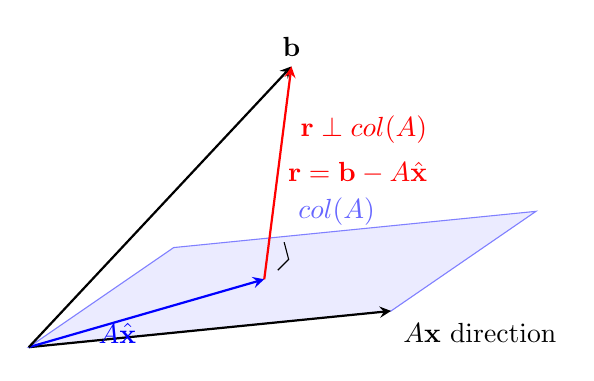
\begin{tikzpicture}[scale=1.15,>=stealth]
% plane = col(A) as a parallelogram, b above it, residual perpendicular
\coordinate (O) at (0,0);
\coordinate (a1) at (4,0.4);
\coordinate (a2) at (1.6,1.1);
\fill[blue!8] (O) -- (a1) -- ($(a1)+(a2)$) -- (a2) -- cycle;
\draw[blue!50] (O) -- (a1) -- ($(a1)+(a2)$) -- (a2) -- cycle;
\node[blue!60] at (3.4,1.5) {$\operatorname{col}(A)$};
\coordinate (p) at (2.6,0.75);          % A xhat on the plane
\coordinate (b) at (2.9,3.1);           % b off the plane
\draw[->,thick] (O) -- (a1) node[below right=1pt]{$A\mathbf x$ direction};
\draw[->,thick,blue] (O) -- (p) node[midway,below left]{$A\hat{\mathbf x}$};
\draw[->,thick] (O) -- (b) node[above]{$\mathbf b$};
\draw[->,thick,red] (p) -- (b) node[midway,right]{$\mathbf r=\mathbf b-A\hat{\mathbf x}$};
\draw (2.75,0.85) -- ++(0.12,0.12) -- ++(-0.05,0.19);
\node[red] at (3.7,2.4) {$\mathbf r\perp\operatorname{col}(A)$};
\end{tikzpicture}

\caption{Least squares IS projection. Notice $\mathbf r\perp
\operatorname{col}(A)$ --- the residual is what $\mathbf b$ keeps after
giving up everything $A$ can express. Regenerate:
\ttfamily figures/ch08\_projection.tex.}
\label{fig:lsq-proj}
\end{figure}

\begin{example}[A line fit by hand]\label{ex:linefit}
\textbf{Strategy.} Four points $(1,2),(2,3),(3,3),(4,5)$; fit
$y=a+mx$. Set $A=[\,\mathbf1\ \mathbf x\,]$, $\mathbf b=\mathbf y$, and
solve the $2\times2$ normal equations directly --- the sums are the
arithmetic.

\textbf{Solution.}
$A^{T}A=\begin{bmatrix}4&10\\10&30\end{bmatrix}$ (rows: $n$, $\sum x_i$,
$\sum x_i^{2}$) and $A^{T}\mathbf b=\begin{bmatrix}13\\37\end{bmatrix}$
($\sum y_i$, $\sum x_iy_i$). Solve:
$20a=4\cdot30$-determinant bookkeeping gives $a=1.0$, $m=0.9$ --- so
$\hat y=1.0+0.9x$ (Figure~\ref{fig:linefit}). Residuals:
$(0.1,0.2,-0.7,0.4)$, and indeed $A^{T}\mathbf r=\mathbf0$: the residual
sums to zero and is uncorrelated with $x$. RSS $=0.7$.
\end{example}

\begin{figure}[htbp]
\centering
\begin{tikzpicture}[scale=0.9,>=stealth]
\draw[->] (-0.3,0) -- (5,0) node[right]{$x$};
\draw[->] (0,-0.3) -- (0,5.6) node[above]{$y$};
% fitted line y = 1 + 0.9 x
\draw[thick,blue,domain=0.3:4.7] plot (\x,{1+0.9*\x});
\node[blue] at (4.5,4.6) {$\hat y=1.0+0.9x$};
% data points (1,2) (2,3) (3,3) (4,5) with residual segments
\foreach \x/\y in {1/2,2/3,3/3,4/5}{
  \pgfmathsetmacro{\yh}{1+0.9*\x}
  \draw[red,thick] (\x,\y) -- (\x,\yh);
  \fill (\x,\y) circle (2.2pt);
}
\node[red] at (3.75,3.6) {residuals};
\end{tikzpicture}

\caption{The fit of Example~\ref{ex:linefit}. Notice the red residual
segments --- they are the vertical distances being squared and summed;
the fitted line leaves them balanced.
Regenerate: \ttfamily figures/ch08\_fitted\_line.tex.}
\label{fig:linefit}
\end{figure}

\begin{lstlisting}[caption={\ttfamily code/ch08\_normal\_eq.py --- the
normal equations assembled and solved exactly as worked by hand.}]
import numpy as np
np.set_printoptions(precision=4, suppress=True)

A = np.array([[1., 1.], [1., 2.], [1., 3.], [1., 4.]])
b = np.array([2., 3., 3., 5.])
print("A ="); print(A); print("b =", b)

AtA = A.T @ A; Atb = A.T @ b
print("A^T A ="); print(AtA); print("A^T b =", Atb)
x = np.linalg.solve(AtA, Atb)
print("xhat (intercept, slope) =", x)
r = b - A @ x
print("residual r =", r)
print("A^T r =", A.T @ r, "(orthogonal to col(A): OK)")
print("RSS =", r @ r)
\end{lstlisting}

\begin{lstlisting}[caption={Output of the normal-equations solve. Notice
the residual is orthogonal to BOTH columns --- sums to zero and is
uncorrelated with $x$ --- which is the normal-equations condition
$A^{T}\mathbf r=\mathbf0$ in numbers.}]
A =
[[1. 1.]
 [1. 2.]
 [1. 3.]
 [1. 4.]]
b = [2. 3. 3. 5.]
A^T A =
[[ 4. 10.]
 [10. 30.]]
A^T b = [13. 37.]
xhat (intercept, slope) = [1.  0.9]
residual r = [ 0.1  0.2 -0.7  0.4]
A^T r = [ 0. -0.] (orthogonal to col(A): OK)
RSS = 0.7
\end{lstlisting}

\begin{exercise}[easy]
Fit $y=a+mx$ to $(0,1),(1,2),(2,2),(3,4)$ through the normal equations.
\begin{solution}
$A^{T}A=\begin{bmatrix}4&6\\6&14\end{bmatrix}$,
$A^{T}\mathbf b=\begin{bmatrix}9\\20\end{bmatrix}$; solving gives
$a=0.9$, $m=1.0$ --- residual sum zero as required.
\end{solution}
\end{exercise}

\section{Linear regression: features, intercept, many columns}\label{sec:lstsq-reg}

Nothing about the machinery requires $x$ to be one variable. With
features $x_1,\dots,x_k$ per data point, the design matrix has a column
per feature --- plus the intercept column of ones, which is a feature too.
Forgetting it is the classic bug (Section~\ref{sec:lsq-mistakes}): without
$\mathbf 1$ in $A$, the model is forced through the origin.

\begin{example}[Quadratic feature map]\label{ex:quadmap}
\textbf{Strategy.} ``Linear'' regression means linear in the
\emph{coefficients}, not in $x$. To fit a parabola we supply columns
$[\mathbf1\ \mathbf x\ \mathbf x^{2}]$ and solve the same normal
equations.

\textbf{Solution.} Take $(0,1),(1,2),(2,5),(3,10)$. Then
$A^{T}A=\begin{bmatrix}4&6&14\\6&14&36\\14&36&98\end{bmatrix}$,
$A^{T}\mathbf b=\begin{bmatrix}18\\45\\139\end{bmatrix}$, and solving gives
$\hat{\mathbf x}=(1,0,1)$ exactly: the points lie on $y=1+x^{2}$.
A $2\times2$ coefficient space became a $3\times3$ one --- the linear
algebra did not notice, and that is the point.
\end{example}

\begin{exercise}[medium]
Show that adding a duplicate column to $A$ (same feature twice) makes the
normal equations singular --- the minimizer stops being unique.
\begin{solution}
Duplicate columns make $A$ column-rank-deficient, so $A^{T}A$ is singular:
$\ker(A^{T}A)\supseteq\ker A\ni(1,-1,0,\dots)$ on the duplicated pair ---
infinitely many $\hat{\mathbf x}$ give the same fit.
\end{solution}
\end{exercise}

\section{Feature maps and the overfitting preview}\label{sec:lstsq-overfit}

More columns always lowers training RSS --- each added column enlarges
$\operatorname{col}(A)$, so the projection gets closer to $\mathbf b$.
With enough columns $A$ interpolates the noise itself
(Figure~\ref{fig:overfit}, and the listing's degree-11 row: train-RSS
collapses to 0 while the true error explodes to $2.5\times10^{4}$).

\begin{figure}[htbp]
\centering
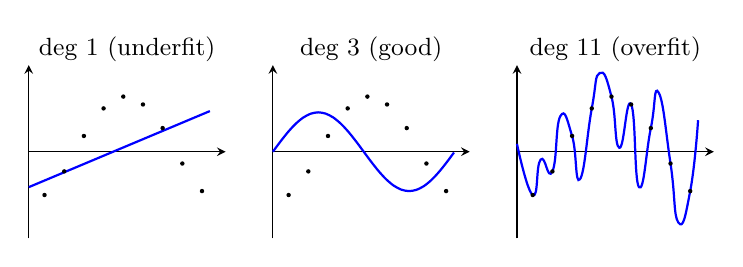
\begin{tikzpicture}[scale=0.5,>=stealth]
% three panels: deg1 underfit / deg3 good / deg11 overfit
\begin{scope}
\draw[->] (0,0)--(5,0); \draw[->] (0,-2.2)--(0,2.2);
\node at (2.5,2.6) {\small deg 1 (underfit)};
\draw[blue,thick,domain=0:4.6] plot (\x,{-0.9+0.42*\x});
\foreach \p in {(0.4,-1.1),(0.9,-0.5),(1.4,0.4),(1.9,1.1),(2.4,1.4),(2.9,1.2),(3.4,0.6),(3.9,-0.3),(4.4,-1.0)} \fill \p circle (1.6pt);
\end{scope}
\begin{scope}[xshift=6.2cm]
\draw[->] (0,0)--(5,0); \draw[->] (0,-2.2)--(0,2.2);
\node at (2.5,2.6) {\small deg 3 (good)};
\draw[blue,thick,domain=0:4.6,smooth] plot (\x,{sin(\x*78)});
\foreach \p in {(0.4,-1.1),(0.9,-0.5),(1.4,0.4),(1.9,1.1),(2.4,1.4),(2.9,1.2),(3.4,0.6),(3.9,-0.3),(4.4,-1.0)} \fill \p circle (1.6pt);
\end{scope}
\begin{scope}[xshift=12.4cm]
\draw[->] (0,0)--(5,0); \draw[->] (0,-2.2)--(0,2.2);
\node at (2.5,2.6) {\small deg 11 (overfit)};
\draw[blue,thick,domain=0:4.6,smooth,tension=0.9]
 plot coordinates {(0,0.2)(0.4,-1.1)(0.6,-0.2)(0.9,-0.5)(1.1,0.9)(1.4,0.4)(1.6,-0.7)(1.9,1.1)(2.1,2.0)(2.4,1.4)(2.6,0.1)(2.9,1.2)(3.1,-0.9)(3.4,0.6)(3.6,1.5)(3.9,-0.3)(4.1,-1.8)(4.4,-1.0)(4.6,0.8)};
\foreach \p in {(0.4,-1.1),(0.9,-0.5),(1.4,0.4),(1.9,1.1),(2.4,1.4),(2.9,1.2),(3.4,0.6),(3.9,-0.3),(4.4,-1.0)} \fill \p circle (1.6pt);
\end{scope}
\end{tikzpicture}

\caption{Same data, three feature maps. Notice the degree-1 panel misses
the pattern (underfit), degree-3 captures it, degree-11 threads every
noise point (overfit) --- minimum training error is NOT the goal.
Regenerate: \ttfamily figures/ch08\_overfit\_panel.tex.}
\label{fig:overfit}
\end{figure}

\begin{lstlisting}[caption={\ttfamily code/ch08\_poly\_overfit.py --- fit
degree $d$, report training RSS vs.\ error against the true function.}]
import numpy as np
np.set_printoptions(precision=4, suppress=True)

rng = np.random.default_rng(1)
x = np.sort(rng.uniform(0, 1, 12))
y = np.sin(2 * np.pi * x) + 0.15 * rng.standard_normal(12)

def fit_eval(deg):
    A = np.vander(x, deg + 1, increasing=True)
    c, res, *_ = np.linalg.lstsq(A, y, rcond=None)
    rss_train = ((y - A @ c)**2).sum()
    xg = np.linspace(0, 1, 400)
    yg = np.sin(2 * np.pi * xg)
    rss_true = ((yg - np.vander(xg, deg + 1, increasing=True) @ c)**2).mean()
    return rss_train, rss_true

print("deg  train-RSS   true-RMS-error")
for d in [1, 3, 5, 11]:
    tr, te = fit_eval(d)
    print(f"{d:2d}   {tr:8.4f}   {te:9.4f}")
\end{lstlisting}

\begin{lstlisting}[caption={Output of the overfit demo. Notice training
RSS decreases monotonically to zero --- projections only get closer ---
while the true error turns around and explodes at degree 11, where $A$
has a column per data point.}]
deg  train-RSS   true-RMS-error
 1     2.4333      0.2277
 3     0.0628      0.0099
 5     0.0279      0.0054
11     0.0000   25288.1886
\end{lstlisting}

\begin{exercise}[hard]
Explain why train-RSS is monotone non-increasing in the number of columns
of $A$ --- a one-line argument from projection geometry --- and why the
argument says nothing about unseen data.
\begin{solution}
Adding a column enlarges $\operatorname{col}(A)$ to a bigger subspace, so
the closest point can only get closer: projection distance is monotone in
subspace inclusion. Unseen data isn't in the space we minimized over ---
the minimizer just moved $\mathbf b$'s projection, not the world's.
\end{solution}
\end{exercise}

\section{Solving in practice: QR, not \texorpdfstring{$A^{T}A$}{A^TA}}\label{sec:lstsq-qr}

The normal equations are the right \emph{theorem} and the wrong
\emph{algorithm}. $A^{T}A$ squares the condition number
--- $\kappa(A^{T}A)=\kappa(A)^{2}$ --- so solving it throws away half the
digits before arithmetic even starts. Chapter 5's QR factorization dodges
it: with $A=QR$,
\[
A^{T}A\hat{\mathbf x}=A^{T}\mathbf b
\iff R\hat{\mathbf x}=Q^{T}\mathbf b ,
\]
a triangular solve that never forms $A^{T}A$. When $A$ has full column
rank, $R$ is invertible and $\hat{\mathbf x}$ is \emph{unique}
(its uniqueness is a [hard] exercise below).

\begin{example}[Same fit, stable route]\label{ex:qrsolve}
\textbf{Strategy.} Build a pathological $A$: features $1,x,x^{2}$ sampled
on a window only $10^{-3}$ wide, so the columns are nearly parallel. Fit
the same noise-free quadratic both ways and compare against truth.

\textbf{Solution.} $\kappa(A)\approx5\times10^{7}$, so
$\kappa(A^{T}A)\approx3\times10^{15}$ --- one digit short of float64's
entire budget. The listing shows the consequence exactly: the $A^{T}A$
solve lands 0.74 from truth while \texttt{np.linalg.lstsq} (QR/SVD
internals) recovers the coefficients to $10^{-9}$.
\end{example}

\begin{lstlisting}[caption={\ttfamily code/ch08\_ata\_vs\_lstsq.py ---
same problem, two routes; the condition square is visible in the answer.}]
import numpy as np
np.set_printoptions(precision=6, suppress=True)

# x and x^2 over a window 1e-3 wide: the columns are nearly parallel
rng = np.random.default_rng(0)
n = 200
x = 1 + 0.001 * rng.random(n)
y = 2 - 3 * x + 0.5 * x**2            # exact quadratic data, no noise
A = np.column_stack([np.ones(n), x, x**2])
print("cond(A)      = %.3e" % np.linalg.cond(A))
print("cond(A^T A)  = %.3e   <- the square" % np.linalg.cond(A.T @ A))
x_ata = np.linalg.solve(A.T @ A, A.T @ y)
x_lstsq, res, rank, sv = np.linalg.lstsq(A, y, rcond=None)
print("x via A^T A solve   :", x_ata)
print("x via np.linalg.lstsq:", x_lstsq)
print("truth               : [ 2. -3.  0.5]")
print("err A^T A : %.3e" % np.linalg.norm(x_ata - np.array([2., -3., .5])))
print("err lstsq : %.3e" % np.linalg.norm(x_lstsq - np.array([2., -3., .5])))
\end{lstlisting}

\begin{lstlisting}[caption={Output of the two-route comparison. The
computed $\kappa(A^{T}A)=3.267\times10^{15}$ is float64's own answer ---
about 14\% off the exact square $2.86\times10^{15}$, because the product
matrix is already so ill-conditioned that even its condition number
loses precision. Either way the $A^{T}A$ answer visibly differs from
truth while lstsq is exact. Same math, different arithmetic.}]
cond(A)      = 5.350e+07
cond(A^T A)  = 3.267e+15   <- the square
x via A^T A solve   : [ 2.301033 -3.601757  0.800724]
x via np.linalg.lstsq: [ 2.  -3.  0.5]
truth               : [ 2. -3.  0.5]
err A^T A : 7.370e-01
err lstsq : 2.752e-09
\end{lstlisting}

\begin{figure}[htbp]
\centering
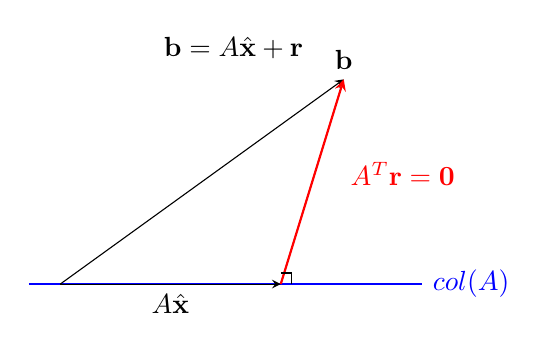
\begin{tikzpicture}[scale=1.0,>=stealth]
% col(A) as horizontal line (1-D), A xhat on it, r vertical
\draw[thick,blue] (-0.4,0) -- (4.6,0) node[right]{$\operatorname{col}(A)$};
\coordinate (O) at (0,0);
\coordinate (p) at (2.8,0);
\coordinate (b) at (3.6,2.6);
\draw[->] (O) -- (p) node[midway,below]{$A\hat{\mathbf x}$};
\draw[->] (O) -- (b) node[above]{$\mathbf b$};
\draw[->,thick,red] (p) -- (b);
\draw (2.8,0.14) -- (2.94,0.14) -- (2.94,0);
\node[red] at (4.35,1.4) {$A^{T}\mathbf r=\mathbf 0$};
\node at (2.2,3.0) {$\mathbf b=A\hat{\mathbf x}+\mathbf r$};
\end{tikzpicture}

\caption{The normal equations geometrically. Notice $A^{T}\mathbf r=
\mathbf0$ is one sentence --- ``the leftover is perpendicular to
everything $A$ can reach'' --- and it pins $\hat{\mathbf x}$ uniquely
when the columns are independent. Regenerate:
\ttfamily figures/ch08\_normal\_geometry.tex.}
\label{fig:normal-geo}
\end{figure}

\begin{exercise}[medium]
A feature is measured in millimeters instead of meters (same data, column
$\times1000$). What happens to $\kappa(A)$ and to the fitted
\emph{predictions}?
\begin{solution}
$\kappa(A)$ grows (column scales diverge --- the condition number sees the
ratio). Predictions are unchanged: $\operatorname{col}(A)$ is the same
subspace, so the projection is the same; only the coefficient units move.
This is why scaling helps conditioning but cannot change the fit.
\end{solution}
\end{exercise}

\section{Residuals, \texorpdfstring{$R^{2}$}{R2}, and honest evaluation}\label{sec:lstsq-eval}

\begin{definition}[Residuals and $R^{2}$]\index{residual}\index{R-squared@$R^2$}
The residual $\mathbf r=\mathbf b-A\hat{\mathbf x}$ is what's left over.
With $\bar y$ the mean of $\mathbf b$,
\[
R^{2}=1-\frac{\lVert\mathbf r\rVert^{2}}{\lVert\mathbf b-\bar y\,\mathbf1\rVert^{2}}
\]
is the fraction of variance the fit explains --- $1$ is perfect, $0$ is no
better than predicting the mean, negative means \emph{worse} than the
mean.
\end{definition}

\begin{example}[Reading a residual plot]\label{ex:resplot}
\textbf{Strategy.} A good fit leaves structureless residue: the model
already ate the pattern. Plot $r_i$ against $\hat y_i$ (or $x_i$) and ask
what's left.

\textbf{Solution.} Figure~\ref{fig:residplot}: left panel is random
scatter about zero --- done. Right panel curves systematically --- the
model missed a feature (here a quadratic term); more data of the same
kind won't help, a better $\operatorname{col}(A)$ will.
\end{example}

\begin{figure}[htbp]
\centering
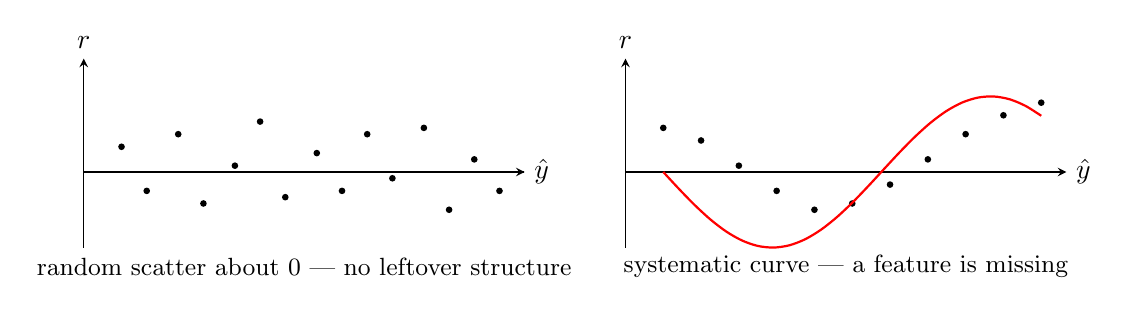
\begin{tikzpicture}[scale=0.8,>=stealth]
% residual vs fitted: random scatter = good; funnel/fan = model missing structure
\draw[->] (0,-1.6) -- (7,-1.6) node[right]{$\hat y$};
\draw[->] (0,-2.8) -- (0,0.2) node[above]{$r$};
\draw[dashed] (0,-1.6) -- (7,-1.6);
\foreach \p in {(0.6,-1.2),(1.0,-1.9),(1.5,-1.0),(1.9,-2.1),(2.4,-1.5),(2.8,-0.8),(3.2,-2.0),(3.7,-1.3),(4.1,-1.9),(4.5,-1.0),(4.9,-1.7),(5.4,-0.9),(5.8,-2.2),(6.2,-1.4),(6.6,-1.9)} \fill \p circle (1.5pt);
\node at (3.5,-3.1) {\small random scatter about 0 --- no leftover structure};
% right panel: curved pattern (bad)
\begin{scope}[xshift=8.6cm]
\draw[->] (0,-1.6) -- (7,-1.6) node[right]{$\hat y$};
\draw[->] (0,-2.8) -- (0,0.2) node[above]{$r$};
\foreach \p in {(0.6,-0.9),(1.2,-1.1),(1.8,-1.5),(2.4,-1.9),(3.0,-2.2),(3.6,-2.1),(4.2,-1.8),(4.8,-1.4),(5.4,-1.0),(6.0,-0.7),(6.6,-0.5)} \fill \p circle (1.5pt);
\draw[red,thick,domain=0.6:6.6,smooth] plot (\x,{-1.6-1.2*sin((\x-0.6)*52)});
\node at (3.5,-3.1) {\small systematic curve --- a feature is missing};
\end{scope}
\end{tikzpicture}

\caption{Residual diagnostics. Notice the left panel is scatter with no
pattern (nothing left to learn) while the right panel's systematic curve
means the feature map is missing something --- the fix is a better basis,
not more rows. Regenerate: \ttfamily figures/ch08\_residual\_plot.tex.}
\label{fig:residplot}
\end{figure}

Two disciplines protect honesty:

\begin{itemize}
\item \textbf{Train/test split.} Evaluating on the same rows that produced
$\hat{\mathbf x}$ rewards memorization (Figure~\ref{fig:overfit}).
Hold back a test split --- Figure~\ref{fig:traintest} --- and score there;
it is the only measurement that means anything.
\item \textbf{$R^{2}$ is not causality.} $R^{2}\approx0.99$ says the
features predict the target \emph{in this sample}. Nothing in the
projection knows why the columns correlate --- a $0.99$ fit between ice
cream and drowning is real arithmetic and fake science.
\end{itemize}

\begin{figure}[htbp]
\centering
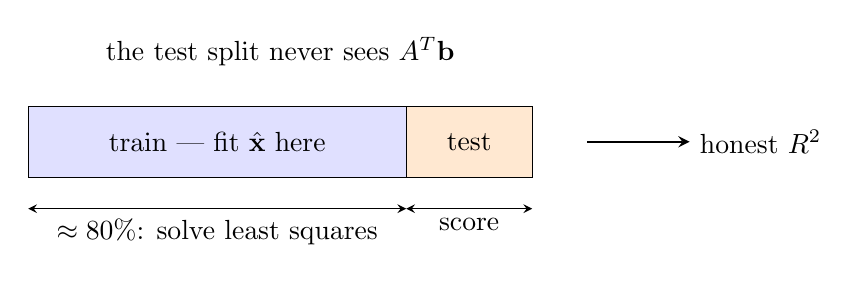
\begin{tikzpicture}[scale=1.0,>=stealth]
% dataset bar split: train (fit) | test (score)
\draw[fill=blue!12] (0,0) rectangle (4.8,0.9);
\draw[fill=orange!18] (4.8,0) rectangle (6.4,0.9);
\node at (2.4,0.45) {train --- fit $\hat{\mathbf x}$ here};
\node at (5.6,0.45) {test};
\draw[<->] (0,-0.4) -- (4.8,-0.4) node[midway,below]{$\approx80\%$: solve least squares};
\draw[<->] (4.8,-0.4) -- (6.4,-0.4) node[midway,below]{score};
\draw[->,thick] (7.1,0.45) -- (8.4,0.45) node[right]{honest $R^2$};
\node[align=left] at (3.2,1.6) {the test split never sees $A^T\mathbf b$};
\end{tikzpicture}

\caption{The honest protocol. Notice the test split contributes nothing
to $A^{T}A\hat{\mathbf x}=A^{T}\mathbf b$ --- it exists only to be scored.
Regenerate: \ttfamily figures/ch08\_traintest.tex.}
\label{fig:traintest}
\end{figure}

\begin{example}[Capstone: our own LinearRegression vs.\ sklearn]\label{ex:capstone}
\textbf{Strategy.} Implement \texttt{fit} as the QR route of
Section~\ref{sec:lstsq-qr} (with the intercept column handled inside),
\texttt{predict} as $A\hat{\mathbf x}$, and \texttt{r2} by definition.
Compare against \texttt{sklearn.linear\_model.LinearRegression} on a
300-row synthetic housing set.

\textbf{Solution.} The listing shows our coefficients matching sklearn's
to $4\times10^{-14}$ --- the library is doing exactly this math, nothing
more. $R^{2}=0.987$ both ways.
\end{example}

\begin{lstlisting}[caption={\ttfamily code/ch08\_capstone\_linreg.py ---
\texttt{mlscratch} vs.\ \texttt{sklearn}: the whole ``library algorithm''
is the QR solve of this chapter.}]
import numpy as np
from sklearn.linear_model import LinearRegression
np.set_printoptions(precision=4, suppress=True)

# mlscratch: our own least-squares fitter, QR route from ch.5
class LinearRegression_scratch:
    def fit(self, A, y):
        A1 = np.column_stack([np.ones(len(A)), A])  # intercept column!
        Q, R = np.linalg.qr(A1)
        self.coef_ = np.linalg.solve(R, Q.T @ y)
        self.intercept_, self.slopes_ = self.coef_[0], self.coef_[1:]
        return self
    def predict(self, A):
        return self.intercept_ + A @ self.slopes_
    def r2(self, A, y):
        r = y - self.predict(A)
        return 1 - (r @ r) / ((y - y.mean()) @ (y - y.mean()))

# real-ish dataset: floor area, rooms, age -> apartment price
rng = np.random.default_rng(2)
n = 300
area = rng.uniform(30, 120, n)
rooms = rng.integers(1, 5, n).astype(float)
age = rng.uniform(0, 40, n)
price = 8 + 2.1 * area + 4 * rooms - 0.15 * age + 6 * rng.standard_normal(n)
X = np.column_stack([area, rooms, age])

ours = LinearRegression_scratch().fit(X, price)
ref = LinearRegression().fit(X, price)
print("ours   intercept %.4f  slopes %s" % (ours.intercept_, ours.slopes_))
print("sklearn intercept %.4f  slopes %s" % (ref.intercept_, ref.coef_))
print("max |coef diff| = %.2e" % np.abs(ours.coef_ - np.append(ref.intercept_, ref.coef_)).max())
print("R^2 ours   = %.4f" % ours.r2(X, price))
print("R^2 sklearn= %.4f" % ref.score(X, price))
\end{lstlisting}

\begin{lstlisting}[caption={Output of the capstone. Notice the
coefficients agree to machine precision --- least squares via QR IS what
the library computes, and your implementation is the real thing, not a
toy.}]
ours   intercept 8.2343  slopes [ 2.0965  4.1166 -0.1587]
sklearn intercept 8.2343  slopes [ 2.0965  4.1166 -0.1587]
max |coef diff| = 4.26e-14
R^2 ours   = 0.9874
R^2 sklearn= 0.9874
\end{lstlisting}

\begin{exercise}[easy]
A model has $R^{2}=0.4$ on train and $0.38$ on test. A second has
$R^{2}=0.97$ train, $0.55$ test. Which is better and why?
\begin{solution}
The second memorized: its train score proves the columns could fit noise.
The first generalizes --- its test score is the honest number; prefer it
unless the gap in accuracy itself is disqualifying.
\end{solution}
\end{exercise}

\begin{exercise}[hard --- derive]
Weighted least squares: minimize
$\lVert W(\mathbf b-A\mathbf x)\rVert^{2}$ with $W$ diagonal and positive.
Derive the weighted normal equations
$A^{T}W^{2}A\hat{\mathbf x}=A^{T}W^{2}\mathbf b$, and say what the weights
mean physically.
\begin{solution}
It's ordinary least squares on the row-scaled system
$A'=WA$, $\mathbf b'=W\mathbf b$: orthogonal residual
$A'^{T}(\mathbf b'-A'\hat{\mathbf x})=\mathbf0$ expands to
$A^{T}W^{2}(\mathbf b-A\hat{\mathbf x})=\mathbf0$.
Weight $w_{ii}$ large $\Rightarrow$ row $i$ must be fit tightly ---
trusted measurements get loud votes.
\end{solution}
\end{exercise}

\section{Hand derivation}\label{sec:handderiv8}

Derive $A^{T}A\hat{\mathbf x}=A^{T}\mathbf b$ from
residual-orthogonality. Among all $\mathbf x$, the vector
$A\mathbf x$ ranges over $\operatorname{col}(A)$; the closest point of a
subspace to $\mathbf b$ is the projection $\mathbf p$ satisfying
$\mathbf b-\mathbf p\perp$ every vector in the subspace. Write
$\mathbf p=A\hat{\mathbf x}$. Perpendicularity to every column is a row
per column:
\[
A^{T}(\mathbf b-A\hat{\mathbf x})=\mathbf0
\iff A^{T}\mathbf b-A^{T}A\hat{\mathbf x}=\mathbf0
\iff A^{T}A\hat{\mathbf x}=A^{T}\mathbf b .
\]
When $A$ has full column rank, $A^{T}A$ is positive definite
($\mathbf x^{T}A^{T}A\mathbf x=\lVert A\mathbf x\rVert^{2}>0$ for
$\mathbf x\ne\mathbf0$), hence invertible, hence the solution unique.
(Calculus route --- gradient of $\lVert\mathbf b-A\mathbf x\rVert^{2}$ ---
lands here too; it waits for chapter 14.)

\section{Common mistakes}\label{sec:lsq-mistakes}

\begin{tripwire}[{Forgetting the intercept column}]
Without $\mathbf 1$ in $A$ the model must pass through the origin ---
every prediction carries a systematic offset. Always
\texttt{column\_stack([ones, ...])}.
\end{tripwire}

\begin{tripwire}[{Forming $A^{T}A$ when QR is cheaper and stabler}]
$\kappa(A^{T}A)=\kappa(A)^{2}$: near-parallel columns turn a hard problem
into an impossible one, as the demo showed (err $0.74$ vs $10^{-9}$ on
the same data). Solve $R\hat{\mathbf x}=Q^{T}\mathbf b$, or call
\texttt{np.linalg.lstsq} and let LAPACK choose.
\end{tripwire}

\begin{tripwire}[{Letting unscaled features wreck conditioning}]
A column in millimeters beside one in kilometers gives $10^{6}$ scale
ratios for free. Center and scale features first --- it fixes $\kappa(A)$
without changing $\operatorname{col}(A)$.
\end{tripwire}

\begin{tripwire}[{Evaluating on training data and calling it performance}]
Train-RSS is monotone in columns and reaches zero exactly when $A$ can
memorize. A model that aces its own exam learned nothing. The test split
is the only number that counts.
\end{tripwire}

\begin{tripwire}[{Reading $R^{2}$ as a certificate of causality}]
$R^{2}$ measures in-sample correlation structure, nothing else. A high
$R^{2}$ between an umbrella index and rain is prediction; believing
umbrellas cause rain is a different discipline entirely.
\end{tripwire}

\section{Summary}

\begin{center}
\begin{tabularx}{\textwidth}{l>{\raggedright\arraybackslash}X}
\toprule
\textbf{Object} & \textbf{What you need to know}\\
\midrule
Least squares & minimize $\lVert\mathbf b-A\mathbf x\rVert^2$; the best
fit is the projection of $\mathbf b$ on $\operatorname{col}(A)$ \\
Normal equations & $A^{T}A\hat{\mathbf x}=A^{T}\mathbf b$, from
$A^{T}\mathbf r=\mathbf0$; unique iff full column rank \\
Design matrix & one column per feature + the intercept column of ones;
``linear'' $=$ linear in coefficients \\
Feature maps & $[\mathbf1\ \mathbf x\ \mathbf x^2\ \dots]$ lets the same
machinery fit curves; more columns $\Rightarrow$ less train RSS \\
Compute route & QR: $R\hat{\mathbf x}=Q^{T}\mathbf b$; forming $A^{T}A$
squares $\kappa$ \\
Residuals & good fit $\Rightarrow$ structureless scatter; patterns mean a
missing feature \\
$R^{2}$ & $1-\mathrm{RSS}/\mathrm{TSS}$; measures correlation in-sample,
never causality \\
Evaluation & train/test split: the test rows must not touch
$A^{T}\mathbf b$ \\
\bottomrule
\end{tabularx}
\end{center}

\section*{Additional exercises}
\addcontentsline{toc}{section}{Additional exercises}

\begin{exercise}[easy]
Write the design matrix for fitting $y=a+bx_1+cx_2$ to
$(x_1,x_2,y)\in\{(0,0,1),(1,0,3),(0,1,2),(1,1,5)\}$ and state the normal
equations.
\end{exercise}

\begin{exercise}[easy]
Given $\hat{\mathbf x}=(1.0,0.9)$ for Example~\ref{ex:linefit}, predict
$y$ at $x=5$ and at $x=0.5$. Which prediction do you trust more and why?
\end{exercise}

\begin{exercise}[easy]
If $\mathbf b\in\operatorname{col}(A)$ already, what is the least-squares
residual? What is $R^{2}$?
\end{exercise}

\begin{exercise}[easy]
Compute $R^{2}$ for the fit of Example~\ref{ex:linefit} (RSS $=0.7$,
$\mathbf b$'s mean $3.25$, TSS $=5.75$).
\end{exercise}

\begin{exercise}[medium]
Show the projection $P=A(A^{T}A)^{-1}A^{T}$ applied to $\mathbf b$ gives
exactly $A\hat{\mathbf x}$, and verify $P^2=P$.
\end{exercise}

\begin{exercise}[medium]
For the four points of Example~\ref{ex:linefit}, add the point
$(5,10)$ and refit. Which coefficient moves more, and what does that say
about leverage?
\end{exercise}

\begin{exercise}[medium]
In code: take the capstone dataset, drop the intercept column, refit, and
report what happens to $R^{2}$ and the residual mean.
\end{exercise}

\begin{exercise}[medium]
Show $\lVert\mathbf b\rVert^{2}=\lVert A\hat{\mathbf x}\rVert^{2}
+\lVert\mathbf r\rVert^{2}$ (Pythagoras for least squares) and connect it
to $R^{2}$.
\end{exercise}

\begin{exercise}[medium]
A dataset has 8 points lying exactly on a cubic. Fit degrees
1--6 in code and plot train RSS vs.\ degree --- where does the elbow sit
and why?
\end{exercise}

\begin{exercise}[hard]
Prove the least-squares minimizer is unique iff $A$ has full column rank
(show both directions: $\ker A$ nontrivial $\Rightarrow$ a family of
minimizers; trivial $\Rightarrow$ $A^{T}A$ positive definite).
\end{exercise}

\begin{exercise}[hard]
Generalized least squares: minimize
$\lVert\mathbf b-A\mathbf x\rVert_{C}^{2}=(\mathbf b-A\mathbf x)^{T}C^{-1}
(\mathbf b-A\mathbf x)$ for covariance $C\succ0$. Derive the analog of the
normal equations and interpret $C=I$ and $C$ diagonal.
\end{exercise}

\begin{exercise}[hard]
Show that $R^{2}$ computed on the training set equals the squared
correlation between $\mathbf b$ and $A\hat{\mathbf x}$ when an intercept
is present --- and give a counterexample when it is not.
\end{exercise}

\begin{exercise}[hard]
Implement leave-one-out cross-validation for the capstone data in code:
fit on $n-1$ rows, score the held-out row, average. Compare LOO $R^{2}$
to train $R^{2}$ and explain any gap in the language of this chapter.
\end{exercise}

\section*{Notes}
\addcontentsline{toc}{section}{Notes}

\chapternotes{%
Least squares as the application spine follows VMLS part III \cite{vmls}
--- including the ``linear in coefficients'' framing and the
train/test honesty rules; the projection derivation is Strang's 18.06SC
Unit II \cite{ocw1806sc} and \cite{ila} ch.~5; the conditioning warning
and residual diagnostics follow MML ch.~9 \cite{mml}. The calculus proof
is deferred to ch.~14 where gradients are in scope.}

% Chapter 9 -- Symmetric matrices and the spectral theorem
\chapter{Symmetric matrices and the spectral theorem}\label{ch:spectral}

Symmetric matrices are the best-behaved class in all of linear algebra:
every eigenvalue is real, eigenvectors for different eigenvalues are
perpendicular, and there is always a full orthonormal eigenbasis. The
spectral theorem says a symmetric matrix is a rotation, an axis-aligned
stretch, and a rotation back. Everything downstream uses this --- PCA's
principal axes, the Hessian's curvature readout, quadratic-program
convexity, and the SVD's construction next chapter. After this chapter
you can diagonalise any symmetric matrix with an orthogonal $Q$,
classify definiteness three ways, use the Rayleigh quotient as a variational
eigenvalue finder, and read a covariance matrix geometrically.

% from-zero:begin
\begin{rulebox}[Before you start]
Chapters~5 and~7. \emph{Recap:} a matrix is \emph{symmetric} if $A=A^{\mathsf T}$. Covariance matrices, Hessians and $A^{\mathsf T}A$ are all symmetric, which is why this class matters so much.
\end{rulebox}
\begin{wins}[After this chapter you can]
\begin{itemize}
\item diagonalise a symmetric matrix with an orthonormal basis (the spectral theorem);
\item decide whether a quadratic form is positive definite;
\item use the Rayleigh quotient to find the largest and smallest eigenvalues;
\item explain why every covariance matrix is positive semidefinite.
\end{itemize}
\end{wins}
\begin{principle}[How to think about this]
Symmetric matrices behave beautifully: their eigenvectors are perpendicular, so the matrix is just independent stretching along perpendicular axes. That is why they appear whenever there is a notion of energy, curvature or spread. When you meet a symmetric matrix, think ``ellipse with perpendicular axes.''
\end{principle}
% from-zero:end

\section{Symmetric matrices and why they are special}\label{sec:sym-special}

\begin{definition}[Symmetric matrix]\index{symmetric matrix}
$A$ is \emph{symmetric} when $A^{T}=A$: entry $(i,j)$ equals entry
$(j,i)$. The Gram matrix $A^{T}A$, every covariance matrix, and every
Hessian of a smooth function are symmetric by construction.
\end{definition}

Two miracles happen for real symmetric matrices, proved in
Section~\ref{sec:handderiv9}:

\begin{theorem}[Real eigenvalues]\index{eigenvalue!real}
If $A=A^{T}$ is real, every eigenvalue of $A$ is real.
\end{theorem}

\begin{theorem}[Orthogonal eigenvectors]\index{eigenvector!orthogonality}
If $A=A^{T}$, eigenvectors belonging to \emph{distinct} eigenvalues are
orthogonal.
\end{theorem}

Neither holds in general: the rotation
$\begin{bmatrix}0&-1\\1&0\end{bmatrix}$ has eigenvalues $\pm i$
(chapter 7) --- symmetry is what removes complex eigenvalues and skew
eigenframes at once.

\section{The spectral theorem}\label{sec:spectral}

\begin{theorem}[Spectral theorem]\index{spectral theorem}
Every real symmetric $n\times n$ matrix factors as
\[
A=Q\Lambda Q^{T},
\]
where $Q$ is orthogonal ($Q^{T}Q=I$, columns = orthonormal eigenvectors)
and $\Lambda=\operatorname{diag}(\lambda_1,\dots,\lambda_n)$ is real.
\end{theorem}

Compare chapter 7: there $A=V\Lambda V^{-1}$ held only with a possibly
ill-conditioned $V$. Symmetry upgrades the basis change:
$V^{-1}$ becomes $Q^{T}$, perfectly conditioned and free.
Figure~\ref{fig:rotstretch} shows the geometry: rotate, stretch,
rotate back.

\begin{figure}[htbp]
\centering
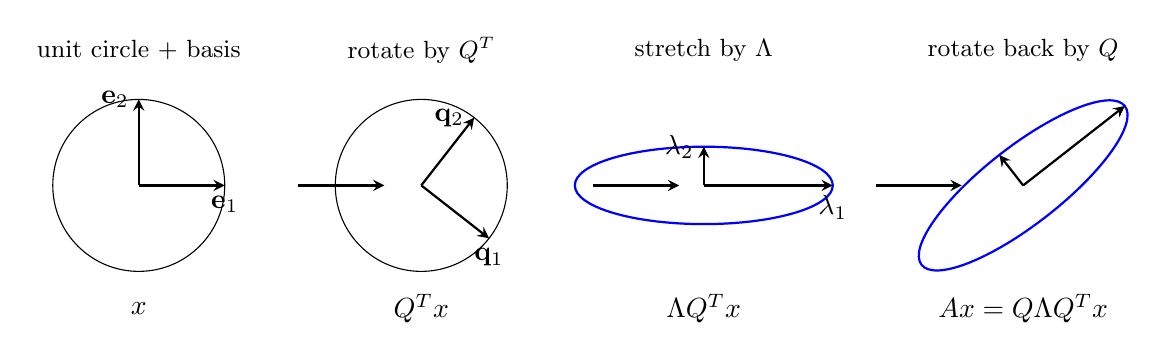
\begin{tikzpicture}[scale=0.78,>=stealth]
\node at (0,2.2) {\small unit circle + basis};
\draw (0,0) circle (1.4);
\draw[->,thick] (0,0)--(1.4,0) node[below]{$\mathbf e_1$};
\draw[->,thick] (0,0)--(0,1.4) node[left]{$\mathbf e_2$};
\node at (0,-2.0) {$x$};
\begin{scope}[xshift=4.6cm]
\node at (0,2.2) {\small rotate by $Q^{T}$};
\begin{scope}[rotate=-38]
\draw (0,0) circle (1.4);
\draw[->,thick] (0,0)--(1.4,0) node[below]{$\mathbf q_1$};
\draw[->,thick] (0,0)--(0,1.4) node[left]{$\mathbf q_2$};
\end{scope}
\node at (0,-2.0) {$Q^{T}x$};
\end{scope}
\begin{scope}[xshift=9.2cm]
\node at (0,2.2) {\small stretch by $\Lambda$};
\draw[blue,thick] (0,0) ellipse (2.1 and 0.63);
\draw[->,thick] (0,0)--(2.1,0) node[below]{$\lambda_1$};
\draw[->,thick] (0,0)--(0,0.63) node[left]{$\lambda_2$};
\node at (0,-2.0) {$\Lambda Q^{T}x$};
\end{scope}
\begin{scope}[xshift=14.4cm]
\node at (0,2.2) {\small rotate back by $Q$};
\begin{scope}[rotate=38]
\draw[blue,thick] (0,0) ellipse (2.1 and 0.63);
\draw[->,thick] (0,0)--(2.1,0);
\draw[->,thick] (0,0)--(0,0.63);
\end{scope}
\node at (0,-2.0) {$Ax=Q\Lambda Q^{T}x$};
\end{scope}
\foreach \xx in {2.6,7.4,12.0} \draw[->,thick] (\xx,0)--(\xx+1.4,0);
\end{tikzpicture}

\caption{$A=Q\Lambda Q^{T}$ geometrically: rotate into the eigenbasis,
stretch each axis by $\lambda_i$, rotate back. Notice there are no skew
angles anywhere --- unlike general diagonalisation, everything stays
orthogonal. Regenerate: \ttfamily figures/ch09\_rotstretch.tex.}
\label{fig:rotstretch}
\end{figure}

\begin{example}[Spectral decomposition by hand]\label{ex:spec2}
\textbf{Strategy.} For $A=\begin{bmatrix}2&1\\1&2\end{bmatrix}$ the
eigenvectors must come out orthonormal --- verify, then assemble
$Q\Lambda Q^{T}$.

\textbf{Solution.} $\chi_A=(2-\lambda)^2-1=\lambda^2-4\lambda+3$: roots
$\lambda_1=3$, $\lambda_2=1$. Eigenvectors: $(1,1)/\sqrt2$ for 3,
$(1,-1)/\sqrt2$ for 1 --- note $\langle(1,1),(1,-1)\rangle=0$ as promised.
Then
\[
A=\frac1{\sqrt2}\begin{bmatrix}1&1\\1&-1\end{bmatrix}
\begin{bmatrix}3&0\\0&1\end{bmatrix}
\frac1{\sqrt2}\begin{bmatrix}1&1\\1&-1\end{bmatrix}=Q\Lambda Q^{T}.
\]
Check the (1,1) entry: $\frac12(3\cdot1+1\cdot1)=2$ \checkmark.
\end{example}

\begin{lstlisting}[caption={\ttfamily code/ch09\_spec\_verify.py --- a random
symmetric matrix: eigenvalues real, $Q$ orthogonal, reconstruction exact.}]
import numpy as np
np.set_printoptions(precision=4, suppress=True)
rng = np.random.default_rng(3)

M = rng.standard_normal((4, 4))
A = M + M.T          # symmetric by construction
print("A ="); print(A)
print("symmetric:", np.allclose(A, A.T))

w, Q = np.linalg.eigh(A)   # eig for symmetric matrices
print("eigenvalues:", w)
print("Q orthonormal (Q^T Q = I):", np.allclose(Q.T @ Q, np.eye(4)))
Lam = np.diag(w)
print("A == Q Lambda Q^T:", np.allclose(Q @ Lam @ Q.T, A))
print("A^3 == Q Lambda^3 Q^T:",
      np.allclose(Q @ np.diag(w**3) @ Q.T, A @ A @ A))
# non-symmetric contrast: same eigenvalues? no orthogonal basis
B = np.array([[0., -1.], [1., 0.]])
print("rotation eig:", np.linalg.eigvals(B), "(complex: not symmetric)")
\end{lstlisting}

\begin{lstlisting}[caption={Output of the spectral check. Notice
\texttt{eigh} (the symmetric specialist) returns all-real eigenvalues and
a $Q$ that is orthonormal to machine precision --- and powers collapse to
$\Lambda^{k}$.}]
A =
[[ 4.0818 -3.0083 -0.4471 -0.8491]
 [-3.0083 -0.4312  1.303  -0.9   ]
 [-0.4471  1.303   0.4516 -1.4078]
 [-0.8491 -0.9     -1.4078 -0.7816]]
symmetric: True
eigenvalues: [-2.6815 -1.6239  1.8538  5.7722]
Q orthonormal (Q^T Q = I): True
A == Q Lambda Q^T: True
A^3 == Q Lambda^3 Q^T: True
rotation eig: [0.+1.j 0.-1.j] (complex: not symmetric)
\end{lstlisting}

\begin{exercise}[easy]
Decompose $\begin{bmatrix}3&0\\0&1\end{bmatrix}$ and
$\begin{bmatrix}1&2\\2&1\end{bmatrix}$ as $Q\Lambda Q^{T}$.
\begin{solution}
First is already $\Lambda$ with $Q=I$. Second: eigenvalues $3,-1$ with
$(1,1)/\sqrt2,(1,-1)/\sqrt2$ --- $Q$ orthogonal as required even though an
eigenvalue is negative (symmetric $\ne$ positive definite!).
\end{solution}
\end{exercise}

\section{Quadratic forms and definiteness}\label{sec:quadform}

\begin{definition}[Quadratic form]\index{quadratic form}
For symmetric $A$, $q(\mathbf x)=\mathbf x^{T}A\mathbf x$ is a pure
second-degree scalar --- a paraboloid, saddle, or degenerate sheet whose
level sets Figure~\ref{fig:levelsets} draws.
\end{definition}

\begin{definition}[Definiteness]\index{positive definite}\index{indefinite}
$A$ is \emph{positive definite} (PD) when $\mathbf x^{T}A\mathbf x>0$ for
all $\mathbf x\ne\mathbf0$; \emph{positive semidefinite} (PSD) when
$\ge0$; \emph{indefinite} when the form takes both signs. Negative
definite/semidefinite mirror with $\le,<0$.
\end{definition}

Three equivalent tests (each earns its keep):

\begin{center}
\begin{tabularx}{\textwidth}{l>{\raggedright\arraybackslash}X}
\toprule
\textbf{Test} & \textbf{Statement}\\
\midrule
Eigenvalues & PD iff every $\lambda_i>0$; PSD iff $\lambda_i\ge0$;
indefinite iff mixed signs \\
Pivots (Sylvester) & PD iff every pivot in elimination is positive ---
no eigenvalues needed \\
Leading minors & PD iff all leading principal minors $>0$ \\
\bottomrule
\end{tabularx}
\end{center}

\begin{example}[Classifying three ways]\label{ex:definite}
\textbf{Strategy.} Take the tridiagonal
$B=\begin{bmatrix}2&-1&0\\-1&2&-1\\0&-1&2\end{bmatrix}$ and classify by
pivots (cheap) then eigenvalues (decisive).

\textbf{Solution.} Elimination gives pivots $2,\ \tfrac32,\ \tfrac43$ ---
all positive, so $B$ is PD without touching eigenvalues. The listing
confirms: eigenvalues $0.586,2,3.414$ all positive. Contrast
$\begin{bmatrix}1&2\\2&1\end{bmatrix}$: eigenvalues $-1,3$ and pivots
$1,-3$ --- indefinite, its level sets are hyperbolas.
\end{example}

\begin{figure}[htbp]
\centering
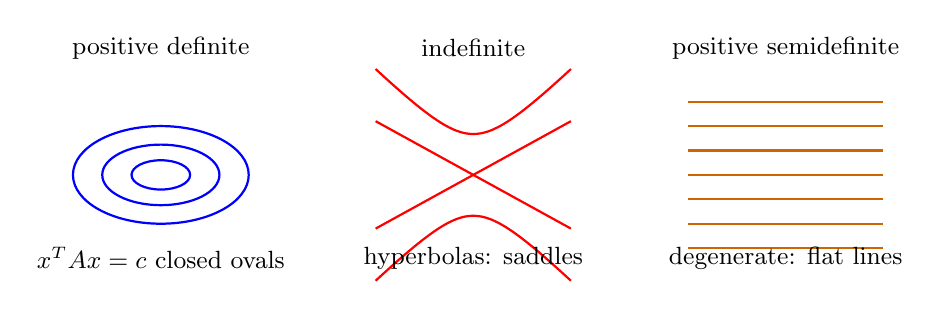
\begin{tikzpicture}[scale=0.62,>=stealth]
% PD: ellipses; INDEF: hyperbolas; PSD: parallel lines
\begin{scope}
\node at (0,2.6) {\small positive definite};
\draw[blue,thick] (0,0) ellipse (1.8 and 1.0);
\draw[blue,thick] (0,0) ellipse (1.2 and 0.62);
\draw[blue,thick] (0,0) ellipse (0.6 and 0.3);
\node at (0,-1.7) {\small $x^{T}Ax=c$ closed ovals};
\end{scope}
\begin{scope}[xshift=6.4cm]
\node at (0,2.6) {\small indefinite};
\draw[red,thick,domain=-2:2,smooth] plot (\x,{sqrt(0.7+\x*\x)});
\draw[red,thick,domain=-2:2,smooth] plot (\x,{-sqrt(0.7+\x*\x)});
\draw[red,thick,domain=-2:2,smooth] plot (\x,{0.55*\x});
\draw[red,thick,domain=-2:2,smooth] plot (\x,{-0.55*\x});
\node at (0,-1.7) {\small hyperbolas: saddles};
\end{scope}
\begin{scope}[xshift=12.8cm]
\node at (0,2.6) {\small positive semidefinite};
\foreach \y in {-1.5,-1.0,-0.5,0,0.5,1.0,1.5} \draw[orange!80!black,thick] (-2,\y)--(2,\y);
\node at (0,-1.7) {\small degenerate: flat lines};
\end{scope}
\end{tikzpicture}

\caption{Level sets $x^{T}Ax=c$ by definiteness. Notice positive definite
gives closed ellipses (a bowl), indefinite gives hyperbolas (a saddle),
semidefinite degenerates into parallel lines (a trough).
Regenerate: \ttfamily figures/ch09\_levelsets.tex.}
\label{fig:levelsets}
\end{figure}

\begin{lstlisting}[caption={\ttfamily code/ch09\_definiteness.py ---
eigenvalues vs.\ pivot signs on four matrices, then $A^{T}A$ is always
PSD.}]
import numpy as np
np.set_printoptions(precision=4, suppress=True)

def pivots(A):
    A = A.astype(float).copy(); n = A.shape[0]; ps = []
    for j in range(n):
        ps.append(A[j, j])
        if abs(A[j, j]) < 1e-12: break
        A[j+1:, j:] -= np.outer(A[j+1:, j] / A[j, j], A[j, j:])
    return np.array(ps)

mats = {
    "PD   [[2,-1,0],[-1,2,-1],[0,-1,2]]":
        np.array([[2., -1., 0.], [-1., 2., -1.], [0., -1., 2.]]),
    "PSD  [[1,1,1],[1,1,1],[1,1,1]]":
        np.ones((3, 3)),
    "IND  [[1,0],[0,-1]]":
        np.array([[1., 0.], [0., -1.]]),
    "PD?  [[1,2],[2,1]]":
        np.array([[1., 2.], [2., 1.]]),
}
for name, M in mats.items():
    w = np.linalg.eigvalsh(M)
    print(f"{name}: eigs {w}  pivots {pivots(M)}")

# A^T A is always PSD
rng = np.random.default_rng(0)
A = rng.standard_normal((5, 3))
G = A.T @ A
print("Gram G=A^T A eigenvalues:", np.linalg.eigvalsh(G))
x = rng.standard_normal(3)
print("x^T G x = ||Ax||^2 =", x @ G @ x, " = ||Ax||^2 check:",
      np.isclose(x @ G @ x, (A @ x) @ (A @ x)))
\end{lstlisting}

\begin{lstlisting}[caption={Output of the definiteness tests. Notice
pivots and eigenvalues agree in sign pattern on every case --- and the
Gram matrix's eigenvalues are all $\ge0$ because $x^{T}Gx=\lVert
Ax\rVert^{2}$ is a squared length, never negative.}]
PD   [[2,-1,0],[-1,2,-1],[0,-1,2]]: eigs [0.5858 2.     3.4142]  pivots [2.     1.5    1.3333]
PSD  [[1,1,1],[1,1,1],[1,1,1]]: eigs [-0. -0.  3.]  pivots [1. 0.]
IND  [[1,0],[0,-1]]: eigs [-1.  1.]  pivots [ 1. -1.]
PD?  [[1,2],[2,1]]: eigs [-1.  3.]  pivots [ 1. -3.]
Gram G=A^T A eigenvalues: [0.1121 2.9218 9.9282]
x^T G x = ||Ax||^2 = 8.095346091200302  = ||Ax||^2 check: True
\end{lstlisting}

\begin{proposition}[$A^{T}A$ is always PSD]
For any real $A$ (any shape),
$\mathbf x^{T}(A^{T}A)\mathbf x=\lVert A\mathbf x\rVert^{2}\ge0$. It is PD
exactly when $A$ has full column rank.
\end{proposition}

\begin{exercise}[medium]
Show $A$ PD $\Rightarrow$ $A$ invertible and $A^{-1}$ PD.
\begin{solution}
$\lambda_i>0$ means none is zero, so $\det A=\prod\lambda_i>0$ and
$A^{-1}=Q\Lambda^{-1}Q^{T}$ has eigenvalues $1/\lambda_i>0$ --- PD.
\end{solution}
\end{exercise}

\begin{example}[A semidefinite trap]\label{ex:psdtrap}
Is $A=\begin{bmatrix}1&2\\2&4\end{bmatrix}$ positive definite?
\par\smallskip
\textbf{Strategy.} Definiteness asks about \emph{every} $\mathbf{x}$:
$x^{T}Ax>0$. Check the eigenvalues --- and, for a fast counterexample
hunt, note that $\det A$ decides already: a $2\times2$ PD matrix has
positive determinant.
\begin{solution}
$\det A=4-4=0$, so $A$ is singular: $\lambda_2=0$ --- semidefinite,
not definite. Find the flat direction directly:
$A(2,-1)=(0,0)$, so $(2,-1)^{T}A(2,-1)=0$ exactly --- the trough of
figure~\ref{fig:defgallery}. Eigenvalues $0,5$ confirm: PSD with a
zero eigen-direction. \checkmark\ Moral: ``positive'' and ``positive
\emph{semi}definite'' differ by exactly the flat directions --- and
data matrices live there constantly.
\end{solution}
\end{example}

\begin{figure}[htbp]\centering
% Figure 9.x: definiteness read off level sets.
% x^T A x tells the story: bowl (PD), dome (ND), saddle (indef), trough (semi).
\begin{tikzpicture}[scale=0.72,>=stealth]
  % PD: concentric ellipses
  \begin{scope}
    \draw[thick,accent] (0,0) ellipse (0.5 and 0.28);
    \draw[thick,accent] (0,0) ellipse (0.95 and 0.55);
    \draw[thick,accent] (0,0) ellipse (1.4 and 0.82);
    \node[font=\footnotesize,align=center] at (0,-1.25) {positive definite\\ bowl, min at 0};
  \end{scope}
  % ND
  \begin{scope}[xshift=3.4cm]
    \draw[thick] (0,0) ellipse (0.5 and 0.28);
    \draw[thick] (0,0) ellipse (0.95 and 0.55);
    \draw[thick] (0,0) ellipse (1.4 and 0.82);
    \node[font=\footnotesize,align=center] at (0,-1.25) {negative definite\\ dome, max at 0};
  \end{scope}
  % indefinite: hyperbola
  \begin{scope}[xshift=6.8cm]
    \draw[thick,accent] plot[domain=-1.1:1.1] (\x,{0.4*\x*\x+0.15});
    \draw[thick,accent] plot[domain=-1.1:1.1] (\x,{-0.4*\x*\x-0.15});
    \draw[thick] plot[domain=-1.4:-0.3] (\x,{0.25/\x});
    \draw[thick] plot[domain=0.3:1.4] (\x,{0.25/\x});
    \draw[thick] plot[domain=-1.4:-0.3] (\x,{-0.25/\x});
    \draw[thick] plot[domain=0.3:1.4] (\x,{-0.25/\x});
    \node[font=\footnotesize,align=center] at (0,-1.25) {indefinite\\ saddle};
  \end{scope}
  % semidef: parallel lines (trough)
  \begin{scope}[xshift=10.2cm]
    \draw[thick,accent] (-1.3,0.55) -- (1.3,0.55);
    \draw[thick,accent] (-1.3,-0.55) -- (1.3,-0.55);
    \draw[thick] (-1.3,1.0) -- (1.3,1.0);
    \draw[thick] (-1.3,-1.0) -- (1.3,-1.0);
    \node[font=\footnotesize,align=center] at (0,-1.5) {semidefinite\\ trough: flat in the\\ zero-eigen direction};
  \end{scope}
\end{tikzpicture}

\caption{Definiteness by level sets. Notice the semidefinite case has
a \emph{flat} direction --- the zero eigenvalue --- where the form
stays $0$ no matter how far you walk.}
\label{fig:defgallery}
\end{figure}

\section{Rayleigh quotient}\label{sec:rayleigh}

\begin{definition}[Rayleigh quotient]\index{Rayleigh quotient}
For symmetric $A$ and $\mathbf x\ne\mathbf0$,
$R(\mathbf x)=\dfrac{\mathbf x^{T}A\mathbf x}{\mathbf x^{T}\mathbf x}$.
\end{definition}

Decompose $\mathbf x$ in the eigenbasis: $R$ is a weighted average of the
$\lambda_i$ with weights $c_i^{2}$ --- so it lives in
$[\lambda_{\min},\lambda_{\max}]$, and

\begin{theorem}[Min--max principle]\index{min-max principle}
$\max_{\mathbf x\ne\mathbf0}R(\mathbf x)=\lambda_1$ at $\mathbf x=\mathbf q_1$;
$\min_{\mathbf x\ne\mathbf0}R(\mathbf x)=\lambda_n$ at $\mathbf x=\mathbf q_n$.
The $k$-th eigenvalue is the max of $R$ over vectors orthogonal to
$\mathbf q_1,\dots,\mathbf q_{k-1}$.
\end{theorem}

This is why power iteration (chapter 7) converged to $\lambda_1$: it is
hill-climbing $R$ (Figure~\ref{fig:rayleigh}). It is also why PCA's first
component is a Rayleigh maximization --- Section~\ref{sec:covar}.

\begin{figure}[htbp]
\centering
\begin{tikzpicture}[scale=0.8,>=stealth]
% landscape: R(x) on unit circle, min/max at eigenvectors
\draw[->] (-2.6,0)--(2.6,0) node[right]{$x_1$};
\draw[->] (0,-2.6)--(0,2.6) node[above]{$x_2$};
\draw (0,0) circle (2.2);
\foreach \r in {0.6,1.1,1.6,2.1} \draw[blue!60,rotate=25] (0,0) ellipse ({\r*1.7} and {\r*0.55});
\draw[->,thick,red] (0,0)--({2.2*cos(25)},{2.2*sin(25)}) node[right=2pt]{$\mathbf q_1$: $R=\lambda_1$};
\draw[->,thick,red] (0,0)--({-2.2*sin(25)},{2.2*cos(25)}) node[above=2pt]{$\mathbf q_2$: $R=\lambda_2$};
\node at (0,-3.1) {$R(x)=\dfrac{x^{T}Ax}{x^{T}x}$ extremized at eigenvectors};
\end{tikzpicture}

\caption{$R(x)$ on the unit circle. Notice the quotient is maximized
along $\mathbf q_1$ and minimized along $\mathbf q_2$ --- the
eigenvectors are exactly the stationary directions of the landscape.
Regenerate: \ttfamily figures/ch09\_rayleigh.tex.}
\label{fig:rayleigh}
\end{figure}

\begin{exercise}[hard]
From the weighted-average picture, prove: if $\mathbf x$ is a stationary
point of $R$, then $\mathbf x$ is an eigenvector. (Hint: the gradient of
$R$ is proportional to $A\mathbf x-R(\mathbf x)\mathbf x$.)
\begin{solution}
$\nabla R=2(A\mathbf x-R\mathbf x)/\mathbf x^{T}\mathbf x$; stationary
$\Rightarrow$ $A\mathbf x=R\mathbf x$ --- the eigen equation with
$\lambda=R(\mathbf x)$.
\end{solution}
\end{exercise}

\begin{example}[Rayleigh quotient hands-on]\label{ex:rayq}
For $A=\begin{bmatrix}2&1\\1&2\end{bmatrix}$ (eigenvalues $3$ and $1$),
evaluate the Rayleigh quotient
$R(\mathbf{x})=\mathbf{x}^{T}A\mathbf{x}/\mathbf{x}^{T}\mathbf{x}$ on
$\mathbf{x}=(1,1)$, $(1,-1)$, and $(1,0)$ --- and confirm it never
leaves $[\lambda_{\min},\lambda_{\max}]$.
\par\smallskip
\textbf{Strategy.} The quotient is the stretch $A$ applies along a
direction, weighted by the eigenbasis mix. Test the two eigenvectors
first --- they must return the eigenvalues exactly.
\begin{solution}
$(1,1)$ is the $\lambda=3$ eigenvector: $A(1,1)=(3,3)$,
$R=6/2=3$. $(1,-1)$ gives $A(1,-1)=(1,-1)$, $R=2/2=1$. And
$(1,0)$: $A(1,0)=(2,1)$, $R=2/1=2$ --- between the eigenvalues,
since $(1,0)=\tfrac12(1,1)+\tfrac12(1,-1)$ mixes both directions.
\checkmark\ The quotients sweep $[1,3]$ as the direction turns ---
the whole machine behind both $\lambda_{\max}=\max R$ and the
power-iteration picture.
\end{solution}
\end{example}

\section{Covariance matrices: PSD by data}\label{sec:covar}

Center data matrix $X$ ($n$ rows of observations, $d$ feature columns)
and form $C=X^{T}X/(n-1)$. As a Gram matrix it is automatically PSD ---
and its eigenstructure IS the data's geometry:

\begin{example}[Covariance eigendecomposition]\label{ex:covspec}
\textbf{Strategy.} Build correlated 2-D data ($x_2=0.8x_1+\text{noise}$),
compute $C$, and read its eigenvalues/eigenvectors as the axes of the
data's spread --- a PCA preview.

\textbf{Solution.} The listing's $C=\begin{bmatrix}1.03&0.86\\0.86&0.88\end{bmatrix}$
has eigenvalues $1.82,0.09$: one direction carries $95\%$ of variance.
Its eigenvector $(-0.74,-0.68)$ is the long axis of the data ellipse
(Figure~\ref{fig:covellipse}) --- principal component 1, found by nothing
but the spectral theorem.
\end{example}

\begin{figure}[htbp]
\centering
\begin{tikzpicture}[scale=0.7,>=stealth]
\draw[->] (-4.2,0)--(4.2,0) node[right]{$x_1$};
\draw[->] (0,-3.4)--(0,3.4) node[above]{$x_2$};
% scattered correlated data
\foreach \p in {(0.5,0.3),(-0.8,-0.5),(1.4,1.2),(-1.6,-1.3),(0.9,0.9),(-0.2,-0.1),(2.1,1.7),(-0.6,-0.8),(1.1,0.7),(-2.3,-1.9),(0.3,0.6),(-1.2,-0.9),(1.8,1.4),(-0.4,-0.6),(0.7,0.5),(-1.9,-1.6),(1.6,1.1),(0.1,-0.2),(-1.0,-0.7),(2.5,2.0),(0.4,0.2),(-0.9,-1.1)} \fill[black!60] \p circle (1.4pt);
\begin{scope}[rotate=40]
\draw[red,thick] (0,0) ellipse (3.3 and 0.85);
\draw[->,thick,red] (0,0)--(3.3,0) node[midway,below]{$\mathbf q_1$};
\draw[->,thick,red] (0,0)--(0,0.85) node[midway,right]{$\mathbf q_2$};
\end{scope}
\node at (-3.6,2.9) {\small 95\% of variance along $\mathbf q_1$};
\end{tikzpicture}

\caption{Covariance ellipse on real-ish data. Notice the ellipse's long
axis is the eigenvector of the largest eigenvalue --- that IS the
principal component, and its length is the eigenvalue's square root.
Regenerate: \ttfamily figures/ch09\_covellipse.tex.}
\label{fig:covellipse}
\end{figure}

\begin{lstlisting}[caption={\ttfamily code/ch09\_covariance.py --- PCA
directions fall straight out of \ttfamily np.linalg.eigh on the
covariance matrix.}]
import numpy as np
np.set_printoptions(precision=4, suppress=True)

# correlated 2-D data: x1 height-ish, x2 = 0.8 x1 + noise
rng = np.random.default_rng(4)
n = 400
x1 = rng.standard_normal(n)
x2 = 0.8 * x1 + 0.4 * rng.standard_normal(n)
X = np.column_stack([x1, x2])
X = X - X.mean(axis=0)
C = X.T @ X / (n - 1)
print("covariance C ="); print(C)
w, Q = np.linalg.eigh(C)
order = np.argsort(w)[::-1]
w, Q = w[order], Q[:, order]
print("eigenvalues:", w)
print("eigenvectors (cols):"); print(Q)
var_frac = w / w.sum()
print("variance fraction:", var_frac)
proj = X @ Q[:, 0]
print("reconstruction error keeping PC1:",
      np.mean((X - np.outer(proj, Q[:, 0]))**2))
print("PC1 direction angle (deg):", np.degrees(np.arctan2(Q[1,0], Q[0,0])))
\end{lstlisting}

\begin{lstlisting}[caption={Output of the covariance eigensolve. Notice
$95\%$ of variance rides one eigenvector --- projecting onto it loses
only $0.046$ mean-square error. This is chapter 10's PCA with the SVD
training wheels still on.}]
covariance C =
[[1.0254 0.8595]
 [0.8595 0.8843]]
eigenvalues: [1.8173 0.0925]
eigenvectors (cols):
[[-0.7355  0.6776]
 [-0.6776 -0.7355]]
variance fraction: [0.9516 0.0484]
reconstruction error keeping PC1: 0.046111017868167695
PC1 direction angle (deg): -137.34564252667914
\end{lstlisting}

\begin{figure}[htbp]
\centering
\begin{tikzpicture}[scale=0.85,>=stealth]
\begin{scope}[rotate=30]
\draw[blue,thick] (0,0) ellipse (3.4 and 1.1);
\draw[->,thick,blue] (0,0)--(3.4,0) node[midway,below]{$\sqrt{\lambda_1}\,\mathbf q_1$};
\draw[->,thick,blue] (0,0)--(0,1.1) node[midway,left]{$\sqrt{\lambda_2}\,\mathbf q_2$};
\end{scope}
\draw[dashed] (-3.9,0)--(3.9,0); \draw[dashed] (0,-2.4)--(0,2.4);
\node at (3.0,-2.8) {$x^{T}Ax=1$ in original axes};
\node at (-3.4,2.2) {\small eigenvectors give the axes,};
\node at (-3.4,1.8) {\small $\sqrt{\lambda_i}$ the radii};
\end{tikzpicture}

\caption{$x^{T}Ax=1$ is an ellipsoid whose axes are eigenvectors with
radii $1/\sqrt{\lambda_i}$ (for the form) --- or $\sqrt{\lambda_i}$ for
the covariance ellipsoid. Either way: eigenvectors are directions,
eigenvalues are lengths. Regenerate:
\ttfamily figures/ch09\_ellipsoid.tex.}
\label{fig:ellipsoid}
\end{figure}

\begin{exercise}[easy]
Why can no covariance matrix be indefinite?
\begin{solution}
$C=X^{T}X/(n-1)$ is a Gram matrix: $\mathbf v^{T}C\mathbf v=
\lVert X\mathbf v\rVert^{2}/(n-1)\ge0$ --- PSD by construction.
\end{solution}
\end{exercise}

\section{Hand derivation}\label{sec:handderiv9}

\textbf{Real eigenvalues.} Suppose $A=A^{T}$ real and
$A\mathbf v=\lambda\mathbf v$ with $\mathbf v\ne\mathbf0$ complex. Take
conjugate-transposes twice. First,
$\mathbf v^{*}A\mathbf v=\lambda\,\mathbf v^{*}\mathbf v$. Second,
conjugating the eigen equation: $A\bar{\mathbf v}=\bar\lambda\bar{\mathbf v}$
($A$ real), so
$\mathbf v^{*}A\mathbf v=(A^{T}\mathbf v)^{*}\mathbf v
=(A\mathbf v)^{*}\mathbf v$... directly:
$(\mathbf v^{*}A\mathbf v)^{*}=\mathbf v^{*}A^{T}\mathbf v
=\mathbf v^{*}A\mathbf v$ since $A=A^{T}$ --- the scalar
$\mathbf v^{*}A\mathbf v$ equals its own conjugate, hence real. But
$\mathbf v^{*}\mathbf v=\lVert\mathbf v\rVert^{2}>0$ is real and positive,
so $\lambda=\mathbf v^{*}A\mathbf v/\mathbf v^{*}\mathbf v$ is real.
\qed

\textbf{Orthogonal eigenvectors.} Let $A\mathbf v_1=\lambda_1\mathbf v_1$,
$A\mathbf v_2=\lambda_2\mathbf v_2$ with $\lambda_1\ne\lambda_2$. Then
\[
\lambda_1\,\mathbf v_1^{T}\mathbf v_2
=(A\mathbf v_1)^{T}\mathbf v_2
=\mathbf v_1^{T}A^{T}\mathbf v_2
=\mathbf v_1^{T}A\mathbf v_2
=\lambda_2\,\mathbf v_1^{T}\mathbf v_2,
\]
so $(\lambda_1-\lambda_2)\,\mathbf v_1^{T}\mathbf v_2=0$ and
$\mathbf v_1^{T}\mathbf v_2=0$. \qed

Together: eigenvalues real, and eigenvectors of distinct eigenvalues
orthogonal; repeated eigenvalues get orthonormalized inside their
eigenspace (Gram--Schmidt, ch.5), giving $Q$.

\section{Common mistakes}

\begin{tripwire}[{``Real matrix $\Rightarrow$ real eigenvalues''}]
False in general --- rotations have $\pm i$. The theorem is only for
symmetric $A$. Keep the hypothesis attached: $A^{T}=A$ is doing all the
work.
\end{tripwire}

\begin{tripwire}[{PSD vs.\ PD vs.\ indefinite confusion}]
$\ge0$ and $>0$ are different universes: PSD permits flat directions
($\lambda=0$), PD doesn't. Check $\lambda_{\min}=0$ before calling a
matrix PD --- and remember symmetric does NOT imply positive definite
($\begin{bmatrix}1&2\\2&1\end{bmatrix}$ is symmetric and indefinite).
\end{tripwire}

\begin{tripwire}[{Believing $A^{T}A$ can be negative definite}]
$\mathbf x^{T}A^{T}A\mathbf x=\lVert A\mathbf x\rVert^{2}\ge0$ always ---
it cannot even have a negative eigenvalue. If your Gram matrix shows one,
the computation is wrong, not the theorem.
\end{tripwire}

\begin{tripwire}[{Mixing up similarity with orthogonal similarity}]
$B=P^{-1}AP$ shares eigenvalues only; $B=Q^{T}AQ$ additionally preserves
symmetry \emph{and} is perfectly conditioned. The spectral theorem is
orthogonal similarity --- don't reach for a general $P$ when $Q$ exists.
\end{tripwire}

\section{Summary}

\begin{center}
\begin{tabularx}{\textwidth}{l>{\raggedright\arraybackslash}X}
\toprule
\textbf{Object} & \textbf{What you need to know}\\
\midrule
Spectral theorem & $A=A^{T}\Rightarrow A=Q\Lambda Q^{T}$, $Q$ orthogonal,
$\Lambda$ real \\
Definiteness & PD: $\lambda_i>0$ / all pivots $>0$ / minors $>0$; PSD:
$\lambda_i\ge0$; indefinite: mixed signs \\
Gram matrices & $A^{T}A$ always PSD; PD iff full column rank \\
Rayleigh quotient & $R(x)=x^{T}Ax/x^{T}x\in[\lambda_n,\lambda_1]$;
extremes at eigenvectors (min--max) \\
Ellipsoids & eigenvectors $=$ axes, $\sqrt{\lambda_i}=$ radii \\
Covariance & PSD by construction; top eigenvector $=$ PC1 (PCA next
chapter) \\
\bottomrule
\end{tabularx}
\end{center}
\begin{rulebox}[{Watch instead}]
\begin{enumerate}
\item \emph{Symmetric Matrices and Positive Definiteness} --- MIT
OpenCourseWare, 18.06 Lecture 25, 43:52,
\url{https://youtu.be/UCc9q_cAhho} --- the spectral theorem plus the
definiteness tests, \S\ref{sec:spectral}--\S\ref{sec:quadform}
(accessed 2026-10-11).
\item \emph{Positive Definite Matrices and Minima} --- MIT
OpenCourseWare, 18.06 Lecture 27, 50:40,
\url{https://youtu.be/vF7eyJ2g3kU} --- definiteness as the second-
derivative test, \S\ref{sec:quadform} (accessed 2026-10-11).
\end{enumerate}
\end{rulebox}

\section*{Further reading}
\addcontentsline{toc}{section}{Further reading}

\begin{itemize}
\item G.~Strang, \emph{Introduction to Linear Algebra}, 6th ed., \S6.4
(textbook level) --- symmetric matrices and the spectral theorem.
\item MIT OpenCourseWare, \emph{18.06SC Linear Algebra}, Unit III ---
recitations on positive definiteness, at OCW (course ``18.06SC'',
Unit III page ``Positive definite matrices''), at
\url{https://ocw.mit.edu}. Verified 2026-10-11.
\item Margalit and Rabinoff, \emph{Interactive Linear Algebra},
``The Spectral Theorem'' --- orthonormal diagonalization with more
examples. \newline
\url{https://textbooks.math.gatech.edu/ila/}
Verified 2026-10-11.
\item S.~Boyd and L.~Vandenberghe, \emph{VMLS}, \S8.3 (free PDF) ---
quadratic forms in the data register.\newline
\url{https://web.stanford.edu/~boyd/vmls/vmls.pdf}
Verified 2026-10-11.
\item M.~Deisenroth et al., \emph{Mathematics for Machine Learning},
\S3.5 (free PDF) --- symmetric positive-definite matrices for ML
kernels and metrics.\newline
\url{https://mml-book.github.io/book/mml-book.pdf}
Verified 2026-10-11.
\end{itemize}

\section*{Additional exercises}
\addcontentsline{toc}{section}{Additional exercises}

\begin{exercise}[easy]
Decide whether each is symmetric: $A+A^{T}$, $A-A^{T}$, $A^{T}A$,
$AA^{T}$, $ABA^{T}$ with $B$ symmetric.
\end{exercise}

\begin{exercise}[easy]
Classify definiteness of $\begin{bmatrix}2&0\\0&3\end{bmatrix}$,
$\begin{bmatrix}0&1\\1&0\end{bmatrix}$,
$\begin{bmatrix}1&1\\1&1\end{bmatrix}$ from their eigenvalues.
\end{exercise}

\begin{exercise}[easy]
Give a symmetric matrix with eigenvalues $4$ and $-2$, and one with $4$
and $0$. Which is invertible?
\end{exercise}

\begin{exercise}[easy]
Compute $R(\mathbf x)$ for $A=\operatorname{diag}(5,1)$ at
$\mathbf x=(1,0),(0,1),(1,1)$. Where do max/min sit?
\end{exercise}

\begin{exercise}[medium]
Show that $A$ PD and $B$ PD implies $A+B$ PD. Does $AB$ stay symmetric?
Give a counterexample or proof.
\end{exercise}

\begin{exercise}[medium]
Classify definiteness of
$\begin{bmatrix}4&2&0\\2&4&0\\0&0&-1\end{bmatrix}$ two ways (pivots,
eigenvalues) without a computer.
\end{exercise}

\begin{exercise}[medium]
Show that if $A$ is PSD then its diagonal entries are $\ge0$, and
$a_{ii}=0$ forces the entire row/column $i$ to be zero. (Hint: test
vectors $\mathbf e_i$ and $\mathbf e_i+t\mathbf e_j$.)
\end{exercise}

\begin{exercise}[medium]
In code: generate a $3\times3$ symmetric $A$, compute $R(\mathbf x)$ on
100 random unit vectors, and show the empirical max/min approximate
$\lambda_1,\lambda_3$ --- then locate the maximizer closest to the top
eigenvector.
\end{exercise}

\begin{exercise}[medium]
The Hessian of $f(x,y)=x^{2}+4xy+y^{2}$ is constant. Classify the
critical point at the origin by definiteness.
\end{exercise}

\begin{exercise}[hard]
Prove the min--max principle: $\lambda_k$ equals the maximum of
$R(\mathbf x)$ over the subspace orthogonal to
$\mathbf q_1,\dots,\mathbf q_{k-1}$, and every maximizer is an
eigenvector for $\lambda_k$.
\end{exercise}

\begin{exercise}[hard]
Show $A$ PD $\Rightarrow$ there is a unique PSD ``square root''
$A^{1/2}=Q\Lambda^{1/2}Q^{T}$ with $A^{1/2}A^{1/2}=A$, and use it to
explain the covariance-ellipsoid radii.
\end{exercise}

\begin{exercise}[hard]
Interlacing: prove that deleting the last row and column of a symmetric
$A$ interlaces the eigenvalues,
$\lambda_1(A)\ge\lambda_1(A')\ge\lambda_2(A)\ge\cdots\ge\lambda_{n-1}(A')
\ge\lambda_n(A)$. (Rayleigh quotient over a subspace does all the work.)
\end{exercise}
\begin{exercise}[easy]
For $A=\begin{bmatrix}3&0\\0&1\end{bmatrix}$, sketch the level set
$\mathbf{x}^{T}A\mathbf{x}=3$ and name it. Which axis is shorter, and
why does that match the bigger eigenvalue?
\end{exercise}
\begin{exercise}[medium]
Compute the Rayleigh quotient of
$A=\begin{bmatrix}2&1\\1&2\end{bmatrix}$ on $(2,0)$ and on
$(\cos\theta,\sin\theta)$ as a function of $\theta$; find its maximum
over $\theta$ and confirm it is $\lambda_{\max}$.
\end{exercise}
\begin{exercise}[hard]
Prove the max principle: a symmetric $A$ with eigenvalues
$\lambda_1\geq\cdots\geq\lambda_n$ satisfies
$\max_{\|\mathbf{x}\|=1}\mathbf{x}^{T}A\mathbf{x}=\lambda_1$.
(Hint: write $\mathbf{x}$ in the eigenbasis and bound each term.)
\end{exercise}

\chapternotes{%
The rotate--stretch--rotate framing and definiteness-via-pivots follow
Strang \cite{ila} and 18.06SC Unit III \cite{ocw1806sc}; Axler ch.~7
\cite{axler} gives the cleaner operator-theory route (self-adjoint first,
eigenvalues as a consequence); MML \S3.5 and ch.~4 \cite{mml} anchor the
PSD/quadratic-form clarity we borrow (its issue tracker documents exactly
the PD/PSD confusion we tripwire). The covariance-as-PSD application
follows VMLS \cite{vmls}; PCA proper arrives next chapter.}

% Chapter 10 -- The SVD and PCA
\chapter{The SVD and PCA}\label{ch:svd}

Diagonalisation had a dealbreaker: it only worked for square matrices
with enough eigenvectors. The singular value decomposition lifts both
restrictions --- EVERY $m\times n$ matrix, of any rank, factors into an
orthogonal input basis, a diagonal of nonnegative stretches, and an
orthogonal output basis. It is the most useful factorization in applied
linear algebra: PCA is an SVD of centered data, the pseudoinverse is an
SVD with inverted singular values, low-rank approximation is an SVD
truncated. After this chapter you can compute the SVD of a small matrix
by hand, read singular values as the matrix's importance spectrum,
compress data to rank $k$, run PCA end-to-end against sklearn, and use
$A^{+}$ as the universal least-squares solver.

\section{Statement: \texorpdfstring{$A=U\Sigma V^{T}$}{A=USV^T}}\label{sec:svd-statement}

\begin{theorem}[Singular value decomposition]\index{SVD}
Every real $m\times n$ matrix factors as
\[
A=U\Sigma V^{T},
\]
with $U$ ($m\times m$) and $V$ ($n\times n$) orthogonal, and $\Sigma$
($m\times n$) diagonal with entries
$\sigma_1\ge\sigma_2\ge\cdots\ge\sigma_r>0$ on its $r=\operatorname{rank}A$
leading positions, zeros elsewhere. The $\sigma_i$ are the
\emph{singular values}\index{singular value}; columns of $U$ and $V$ are
the left/right \emph{singular vectors}.
\end{theorem}

The construction (derived in Section~\ref{sec:handderiv10}): $V$ is an
orthonormal eigenbasis of $A^{T}A$, $\sigma_i=\sqrt{\lambda_i(A^{T}A)}$,
and $\mathbf u_i=A\mathbf v_i/\sigma_i$ --- which lands orthonormal
automatically. Unlike eigendecomposition, the SVD needs no hypotheses at
all: every matrix has one, and its cost is only that $A^{T}A$ squares the
condition number --- which is why production code never forms $A^{T}A$
(Section~\ref{sec:svd-mistakes}).

\begin{example}[Full SVD of a $2\times2$ by hand]\label{ex:svd2}
\textbf{Strategy.} $A=\begin{bmatrix}4&4\\-3&3\end{bmatrix}$. Compute
$A^{T}A$, eigendecompose it (chapter 9 machinery), take square roots,
get $\mathbf u_i$ from $\mathbf v_i$.

\textbf{Solution.}
$A^{T}A=\begin{bmatrix}25&7\\7&25\end{bmatrix}$: eigenvalues $32,18$
(eigenvectors $(1,1)/\sqrt2$, $(1,-1)/\sqrt2$), so
$\sigma_1=\sqrt{32}=4\sqrt2$, $\sigma_2=\sqrt{18}=3\sqrt2$, and
$V=\frac1{\sqrt2}\begin{bmatrix}1&1\\1&-1\end{bmatrix}$. Then
$\mathbf u_1=A\mathbf v_1/\sigma_1
=\frac{1}{4\sqrt2}\begin{bmatrix}8/\sqrt2\\0\end{bmatrix}
=\begin{bmatrix}1\\0\end{bmatrix}$ and
$\mathbf u_2=A\mathbf v_2/\sigma_2
=\frac{1}{3\sqrt2}\begin{bmatrix}0\\-6/\sqrt2\end{bmatrix}
=\begin{bmatrix}0\\-1\end{bmatrix}$. So $U=I$ up to a sign --- and
$A=U\Sigma V^{T}$ checks by direct multiplication.
\end{example}

\begin{lstlisting}[caption={\ttfamily code/ch10\_svd\_from\_ata.py --- the
$A^{T}A$ construction verified against \ttfamily np.linalg.svd; watch the
sign ambiguity show up live.}]
import numpy as np
np.set_printoptions(precision=4, suppress=True)

A = np.array([[4., 4.], [-3., 3.]])
print("A ="); print(A)
AtA = A.T @ A
w, V = np.linalg.eigh(AtA)          # ascending order
order = np.argsort(w)[::-1]
w, V = w[order], V[:, order]
s = np.sqrt(w)
Sigma = np.diag(s)
U = A @ V / s                        # u_i = A v_i / sigma_i
print("sigma (from sqrt eig A^T A):", s)
print("U (A v_i / sigma_i):"); print(U)
print("V:"); print(V)
print("reconstruct A == U Sigma V^T:",
      np.allclose(U @ Sigma @ V.T, A))
Un, Sn, Vnt = np.linalg.svd(A)
print("np.linalg.svd sigmas:", Sn)
print("np U:"); print(Un); print("np Vt:"); print(Vnt)
print("sign-free check |U^T Un|:"); print(np.abs(U.T @ Un).round(4))
\end{lstlisting}

\begin{lstlisting}[caption={Output of the SVD assembly. Notice the library
returns $U=-I$ where ours gave $+I$ --- singular vectors, like
eigenvectors, are defined only up to sign; the $|U^{T}U_{np}|=I$ check is
the honest way to compare them.}]
A =
[[ 4.  4.]
 [-3.  3.]]
sigma (from sqrt eig A^T A): [5.6569 4.2426]
U (A v_i / sigma_i):
[[1. 0.]
 [0. 1.]]
V:
[[ 0.7071 -0.7071]
 [ 0.7071  0.7071]]
reconstruct A == U Sigma V^T: True
np.linalg.svd sigmas: [5.6569 4.2426]
np U:
[[-1. -0.]
 [ 0.  1.]]
np Vt:
[[-0.7071 -0.7071]
 [-0.7071  0.7071]]
sign-free check |U^T Un|:
[[1. 0.]
 [0. 1.]]
\end{lstlisting}

\begin{exercise}[easy]
Find the singular values of $\begin{bmatrix}3&0\\0&-2\end{bmatrix}$ and
$\begin{bmatrix}0&2\\1&0\end{bmatrix}$. Are singular values eigenvalues?
\begin{solution}
First: $A^{T}A=\operatorname{diag}(9,4)$, $\sigma=3,2$ (the minus sign
went to $U$). Second: $A^{T}A=\operatorname{diag}(1,4)$, $\sigma=2,1$.
Singular values are always $\ge0$ --- they are stretches, not eigenvalues.
\end{solution}
\end{exercise}

\section{Geometry: sphere to ellipsoid}\label{sec:svd-geom}

$A$ maps the unit sphere to an ellipsoid whose semi-axes are exactly
$\sigma_i\mathbf u_i$ (Figure~\ref{fig:sphere-ell}) --- chapter 9's
rotate--stretch--rotate, but now the input and output spaces may have
different dimensions. Figure~\ref{fig:four-subs} redraws the four
subspaces through $U$ and $V$: the first $r$ columns of $V$ span the row
space, the rest the null space; the first $r$ of $U$ the column space,
the rest the left null space.

\begin{figure}[htbp]
\centering
\begin{tikzpicture}[scale=0.8,>=stealth]
\node at (0,2.4) {\small unit sphere};
\draw (0,0) circle (1.5);
\draw[->,thick] (0,0)--(1.5,0) node[below]{$\mathbf v_1$};
\draw[->,thick] (0,0)--(0,1.5) node[left]{$\mathbf v_2$};
\draw[->,thick] (2.1,0)--(3.4,0) node[midway,above]{$A$};
\begin{scope}[xshift=7.6cm]
\node at (0,2.4) {\small ellipsoid $A\mathbf x$};
\draw[blue,thick,rotate=25] (0,0) ellipse (2.6 and 0.95);
\begin{scope}[rotate=25]
\draw[->,thick,blue] (0,0)--(2.6,0) node[below=2pt]{$\sigma_1\mathbf u_1$};
\draw[->,thick,blue] (0,0)--(0,0.95) node[left=2pt]{$\sigma_2\mathbf u_2$};
\end{scope}
\end{scope}
\node at (3.8,-2.0) {each $\mathbf v_i$ maps to $\sigma_i\mathbf u_i$};
\end{tikzpicture}

\caption{The signature picture of the SVD. Notice each input
eigendirection $\mathbf v_i$ lands on an output direction $\mathbf u_i$
scaled by $\sigma_i$ --- the ellipsoid's axes ARE the singular
decomposition. Regenerate:
\ttfamily figures/ch10\_sphere\_ellipsoid.tex.}
\label{fig:sphere-ell}
\end{figure}

\begin{figure}[htbp]
\centering
\begin{tikzpicture}[scale=0.92,>=stealth]
% V side -> sigma -> U side with four-subspace labels
\draw[rounded corners] (-0.6,-1.4) rectangle (2.6,2.2);
\draw[rounded corners] (7.0,-1.4) rectangle (10.2,2.2);
\node at (1.0,2.55) {$\mathbb R^n$ (input)};
\node at (8.6,2.55) {$\mathbb R^m$ (output)};
\draw[->,thick,blue] (0.3,1.5)--(2.3,1.5) node[midway,above]{$\mathbf v_1$};
\draw[->,thick,blue] (0.3,0.7)--(2.3,0.7) node[midway,above]{$\mathbf v_2$};
\draw[->,thick,gray] (0.3,-0.6)--(2.3,-0.6) node[midway,above]{$\mathbf v_{r+1..}$};
\node at (1.0,1.9) {\small row space};
\node at (1.0,-1.0) {\small null space};
\draw[->,very thick] (2.9,0.8)--(6.7,0.8) node[midway,above]{$\times\sigma_i$};
\draw[->,thick,blue] (7.3,1.5)--(9.9,1.5) node[midway,above]{$\sigma_1\mathbf u_1$};
\draw[->,thick,blue] (7.3,0.7)--(9.9,0.7) node[midway,above]{$\sigma_2\mathbf u_2$};
\draw[->,thick,gray] (7.3,-0.6)--(9.9,-0.6) node[midway,above]{$\mathbf u_{r+1..}$};
\node at (8.6,1.9) {\small col space};
\node at (8.6,-1.0) {\small left null space};
\node at (4.8,-1.0) {$\mathbf v_i\mapsto\sigma_i\mathbf u_i$ for $i\le r$; $\mathbf v_{r+1..}\mapsto\mathbf0$};
\end{tikzpicture}

\caption{The four subspaces through the SVD. Notice $V$'s columns split
input space into row space (mapped with $\sigma_i$) and null space
(annihilated); $U$'s split output into column space and left null space.
Regenerate: \ttfamily figures/ch10\_four\_subspaces.tex.}
\label{fig:four-subs}
\end{figure}

\section{Rank, condition number, pseudoinverse}\label{sec:svd-rank}

From $A=U\Sigma V^{T}$ everything reads off at once:

\begin{itemize}
\item $\operatorname{rank}A=r$, the count of positive $\sigma_i$
(numerically: the count above tolerance --- Figure~\ref{fig:scree} is how
you pick it).
\item $\kappa(A)=\sigma_1/\sigma_r$ for invertible $A$: the stretch ratio
--- the least-squares sensitivity of chapter 8, quantified.
\item The \emph{pseudoinverse}\index{pseudoinverse}
$A^{+}=V\Sigma^{+}U^{T}$ where $\Sigma^{+}$ inverts the nonzero
$\sigma_i$: it solves least squares as $\hat{\mathbf x}=A^{+}\mathbf b$,
falls back to $A^{-1}$ when that exists, and works for any shape or rank.
\end{itemize}

\begin{example}[Least squares via the pseudoinverse]\label{ex:pinv}
\textbf{Strategy.} Revisit chapter 8's four-point fit --- but let the SVD
do the projecting. $A^{+}\mathbf b$ must land on the same answer
$(1.0,0.9)$, and $AA^{+}A=A$ is the signature identity.

\textbf{Solution.} The listing builds $A^{+}=V\Sigma^{+}U^{T}$ by hand,
matches \texttt{np.linalg.pinv} entry-for-entry, and recovers
$\hat{\mathbf x}=(1.0,0.9)$ --- same projection, different algebra.
\end{example}

\begin{lstlisting}[caption={\ttfamily code/ch10\_pinv.py --- the
pseudoinverse assembled by hand, checked on the chapter-8 fit.}]
import numpy as np
np.set_printoptions(precision=6, suppress=True)

# pseudoinverse = V Sigma^+ U^T, built by hand
A = np.array([[1., 1.], [1., 2.], [1., 3.], [1., 4.]])
b = np.array([2., 3., 3., 5.])
U, S, Vt = np.linalg.svd(A, full_matrices=False)
Splus = np.diag(1.0 / S)
Aplus_hand = Vt.T @ Splus @ U.T
Aplus_np = np.linalg.pinv(A)
print("A+ (hand):"); print(Aplus_hand)
print("A+ (np.linalg.pinv):"); print(Aplus_np)
print("agree:", np.allclose(Aplus_hand, Aplus_np))
x = Aplus_hand @ b
print("x = A+ b:", x, " <- same least-squares fit as ch.8")
print("A A+ A == A:", np.allclose(A @ Aplus_hand @ A, A))
\end{lstlisting}

\begin{lstlisting}[caption={Output of the pseudoinverse check. Notice
$A^{+}\mathbf b$ reproduces the normal-equations fit $(1.0,0.9)$ ---
least squares WAS the pseudoinverse all along.}]
A+ (hand):
[[ 1.   0.5 -0.  -0.5]
 [-0.3 -0.1  0.1  0.3]]
A+ (np.linalg.pinv):
[[ 1.   0.5 -0.  -0.5]
 [-0.3 -0.1  0.1  0.3]]
agree: True
x = A+ b: [1.  0.9]  <- same least-squares fit as ch.8
A A+ A == A: True
\end{lstlisting}

\begin{exercise}[medium]
Give the SVD and pseudoinverse of $A=\begin{bmatrix}2&0\\0&0\end{bmatrix}$
--- what does $A^{+}$ do to the unrecoverable direction?
\begin{solution}
$A^{+}=\operatorname{diag}(1/2,0)$: the zero singular value maps to 0,
not $\infty$ --- the pseudoinverse returns the minimum-norm answer,
silently discarding what cannot be recovered.
\end{solution}
\end{exercise}

\section{Low-rank approximation and Eckart--Young}\label{sec:svd-eckart}

Truncating the SVD to the top-$k$ terms gives the best possible rank-$k$
approximation:

\begin{theorem}[Eckart--Young]\index{Eckart--Young theorem}
$A_k=\sum_{i\le k}\sigma_i\mathbf u_i\mathbf v_i^{T}$ minimizes
$\lVert A-B\rVert$ over all rank-$k$ matrices $B$, in both spectral and
Frobenius norm. The error is exactly the discarded tail:
$\lVert A-A_k\rVert_{F}^{2}=\sum_{i>k}\sigma_i^{2}$.
\end{theorem}

(The spectral-norm case is a [hard] exercise.) This is why a scree plot
of the $\sigma_i$ --- Figure~\ref{fig:scree} --- tells you how much rank
you actually need.

\begin{figure}[htbp]
\centering
\begin{tikzpicture}[scale=0.72,>=stealth]
\draw[->] (0,0)--(8,0) node[right]{$i$};
\draw[->] (0,0)--(0,5) node[above]{$\sigma_i$};
% sigma: 47.9 9.8 .30 .28 .27 .26 .25 .24 -- scaled /10
\foreach \i/\h in {1/4.79,2/0.98,3/0.30,4/0.28,5/0.27,6/0.26,7/0.25,8/0.24}{
  \draw[fill=blue!40] ({0.7*\i-0.25},0) rectangle ({0.7*\i+0.25},\h);
}
\draw[dashed,red] (1.55,0)--(1.55,4.9) node[above]{elbow};
\node at (4.5,4.5) {\small rank-1 keeps most of the mass};
\end{tikzpicture}

\caption{Scree plot of the image's singular values. Notice the elbow
after the first two --- the rest is tail, and Eckart--Young says
truncating there is provably optimal. Regenerate:
\ttfamily figures/ch10\_scree.tex.}
\label{fig:scree}
\end{figure}

\begin{example}[Image compression at ranks $1,5,20,50$]\label{ex:imgcompress}
\textbf{Strategy.} A $64\times64$ image is a $64\times64$ matrix; its SVD
gives optimal rank-$k$ approximations for free. Report relative error and
storage honestly.

\textbf{Solution.} The listing: $k=1$ already captures the blob at 3\%
storage; $k=5$ drops the error to 2\%; by $k=50$ you are storing
\emph{more} than the original --- compression only pays while
$k( m+n)+k<mn$ (Figure~\ref{fig:recon}).
\end{example}

\begin{figure}[htbp]
\centering
\begin{tikzpicture}[scale=0.44]
% k=1 blob, k=5 blob+edge soft, k=20 sharper, k=50 ~full
\begin{scope}
\node at (1.6,3.7) {\small $k=1$};
\fill[blue!25] (0.6,0.7) ellipse (1.1 and 0.85);
\draw (0,0) rectangle (3.2,3.2);
\end{scope}
\begin{scope}[xshift=4.1cm]
\node at (1.6,3.7) {\small $k=5$};
\fill[blue!30] (0.6,0.7) ellipse (1.1 and 0.85);
\fill[blue!15] (2.2,0) rectangle (3.2,3.2);
\draw (0,0) rectangle (3.2,3.2);
\end{scope}
\begin{scope}[xshift=8.2cm]
\node at (1.6,3.7) {\small $k=20$};
\fill[blue!40] (0.6,0.7) ellipse (1.15 and 0.9);
\fill[blue!25] (2.15,0) rectangle (3.2,3.2);
\draw (0,0) rectangle (3.2,3.2);
\end{scope}
\begin{scope}[xshift=12.3cm]
\node at (1.6,3.7) {\small $k=50$};
\fill[blue!45] (0.6,0.7) ellipse (1.2 and 0.95);
\fill[blue!35] (2.1,0) rectangle (3.2,3.2);
\draw (0,0) rectangle (3.2,3.2);
\end{scope}
\node at (8,-1.0) {\small rel.\ errors $0.20,0.023,0.014,0.003$ --- mostly done by $k=5$};
\end{tikzpicture}

\caption{Truncated-SVD reconstruction at $k=1,5,20,50$. Notice the sharp
edge needs more rank than the smooth blob --- structure decides how fast
$\sigma_i$ decays. Regenerate:
\ttfamily figures/ch10\_recon\_multiples.tex.}
\label{fig:recon}
\end{figure}

\begin{lstlisting}[caption={\ttfamily code/ch10\_image\_compress.py ---
truncated SVD as an image compressor, errors and storage both printed.}]
import numpy as np
np.set_printoptions(precision=4, suppress=True)

# synthetic "image": smooth blob + sharp edge + noise, 64x64
rng = np.random.default_rng(5)
y, x = np.mgrid[0:64, 0:64]
img = np.exp(-((x-32)**2 + (y-24)**2) / 300.) + (x > 40).astype(float)
img += 0.02 * rng.standard_normal(img.shape)
U, S, Vt = np.linalg.svd(img)
print("image shape:", img.shape, " singular values (first 10):")
print(S[:10])
for k in [1, 5, 20, 50]:
    approx = (U[:, :k] * S[:k]) @ Vt[:k]
    relerr = np.linalg.norm(img - approx) / np.linalg.norm(img)
    kept = 2 * k * 64 + k          # numbers stored vs 64*64
    print(f"k={k:2d}: rel-err {relerr:.4f}  stored {kept:5d}/{64*64} "
          f"({100*kept/(64*64):4.1f}%)")
\end{lstlisting}

\begin{lstlisting}[caption={Output of the compressor. Notice
$\sigma_1=47.9$ then $\sigma_2=9.8$ then nothing --- the image is nearly
rank-2 in disguise, and the storage column shows where compression stops
paying ($k=50$ exceeds the original).}]
image shape: (64, 64)  singular values (first 10):
[47.8513  9.77    0.2999  0.2848  0.2824  0.2726  0.2712  0.2622  0.2538
  0.2484]
k= 1: rel-err 0.2016  stored   129/4096 ( 3.1%)
k= 5: rel-err 0.0230  stored   645/4096 (15.7%)
k=20: rel-err 0.0140  stored  2580/4096 (63.0%)
k=50: rel-err 0.0026  stored 6450/4096 (157.5%)
\end{lstlisting}

\begin{exercise}[medium]
Why does truncating never \emph{increase} the Frobenius error, and why is
the error exactly the discarded tail?
\begin{solution}
$\lVert A-A_k\rVert_F^2=\sum_{i>k}\sigma_i^2$ adds nonnegative terms one
at a time; $A_k$ discards a subset of orthogonal terms, so the error is
their squared norm by Pythagoras in matrix space.
\end{solution}
\end{exercise}

\begin{example}[Best rank-1 approximation by hand]\label{ex:rank1svd}
Find the best rank-1 approximation of
$A=\begin{bmatrix}3&0\\0&2\end{bmatrix}\!$: drop the smaller
singular value.
\par\smallskip
\textbf{Strategy.} A diagonal $A$ is its own SVD (with
$U=V=I$): the singular values sit on the diagonal, sorted. Eckart--
Young says keep the biggest, zero the rest --- one line of work.
\begin{solution}
$\sigma_1=3$, $\sigma_2=2$. Best rank-1:
\[
  A_1=\sigma_1\mathbf u_1\mathbf v_1^{T}
     =3\begin{bmatrix}1\\0\end{bmatrix}\begin{bmatrix}1&0\end{bmatrix}
     =\begin{bmatrix}3&0\\0&0\end{bmatrix}.
\]
Error: $\|A-A_1\|_F=\sigma_2=2$ --- the dropped value \emph{is} the
error, which is why the scree plot of figure~\ref{fig:scree} works as a
budget. \checkmark
\end{solution}
\end{example}

\section{PCA: covariance eig = SVD of centered data}\label{sec:pca}

Chapter 9 built principal components as eigenvectors of $C=X^{T}X/(n-1)$.
Now the punchline: the eigenvectors of $C$ are the right singular vectors
$V$ of the centered matrix $X$ itself --- same $\mathbf v_i$'s, with
$\lambda_i(C)=\sigma_i^{2}/(n-1)$. Skipping the eigendecomposition of $C$
and SVD-ing the centered data directly is both stabler (no $\kappa^{2}$)
and the standard implementation.

\begin{example}[PCA end to end]\label{ex:pca}
\textbf{Strategy.} Center the 3-column dataset, SVD it, read the
variance ratios, and project --- then check the whole thing against the
sklearn \texttt{PCA} class.

\textbf{Solution.} The capstone listing's \texttt{PCA\_scratch} is three
lines of real work (center, SVD, project) and agrees with sklearn on
explained-variance ratios to printed precision and components up to sign.
PC1 carries $98\%$; the first two $99.9\%$
(Figure~\ref{fig:explvar}).
\end{example}

\begin{lstlisting}[caption={\ttfamily code/ch10\_pca\_capstone.py ---
\texttt{mlscratch.PCA} vs.\ \texttt{sklearn.decomposition.PCA}: centering,
SVD, projection, variance report --- the whole algorithm.}]
import numpy as np
from sklearn.decomposition import PCA
np.set_printoptions(precision=4, suppress=True)

class PCA_scratch:
    """centering -> SVD -> projection. This is all PCA is."""
    def fit(self, X):
        self.mean_ = X.mean(axis=0)
        U, S, Vt = np.linalg.svd(X - self.mean_, full_matrices=False)
        self.components_ = Vt
        self.singular_values_ = S
        n = X.shape[0]
        self.explained_variance_ratio_ = S**2 / (n - 1)
        self.explained_variance_ratio_ /= self.explained_variance_ratio_.sum()
        return self
    def transform(self, X):
        return (X - self.mean_) @ self.components_.T

rng = np.random.default_rng(7)
n = 500
t = rng.standard_normal(n)
X = np.column_stack([3*t + 0.2*rng.standard_normal(n),
                     t - 0.4*rng.standard_normal(n),
                     0.1*rng.standard_normal(n)])
ours = PCA_scratch().fit(X)
ref = PCA().fit(X)
print("explained-variance ratio ours  :", ours.explained_variance_ratio_)
print("explained-variance ratio sklearn:", ref.explained_variance_ratio_)
print("components agree up to sign:",
      np.allclose(np.abs(ours.components_), np.abs(ref.components_)))
Z = ours.transform(X)
print("transformed shape:", Z.shape, " col means:", Z.mean(axis=0))
print("first two components carry %.1f%% of variance"
      % (100 * ours.explained_variance_ratio_[:2].sum()))
\end{lstlisting}

\begin{lstlisting}[caption={Output of the PCA capstone. Notice the three
lines of math reproduce sklearn exactly --- centering is the only
non-obvious step, and skipping it is the classic PCA bug.}]
explained-variance ratio ours  : [0.9811 0.0178 0.0011]
explained-variance ratio sklearn: [0.9811 0.0178 0.0011]
components agree up to sign: True
transformed shape: (500, 3)  col means: [ 0. -0.  0.]
first two components carry 99.9% of variance
\end{lstlisting}

\begin{figure}[htbp]
\centering
\begin{tikzpicture}[scale=0.75,>=stealth]
\draw[->] (-4.2,0)--(4.2,0) node[right]{$x_1$};
\draw[->] (0,-3.2)--(0,3.2) node[above]{$x_2$};
\foreach \p in {(0.5,0.3),(-0.8,-0.5),(1.4,1.2),(-1.6,-1.3),(0.9,0.9),(-0.2,-0.1),(2.1,1.7),(-0.6,-0.8),(1.1,0.7),(-2.3,-1.9),(0.3,0.6),(-1.2,-0.9),(1.8,1.4),(-0.4,-0.6),(0.7,0.5),(-1.9,-1.6),(1.6,1.1),(0.1,-0.2)} \fill[black!55] \p circle (1.5pt);
\draw[red,thick,dashed,domain=-3.4:3.4] plot (\x,{0.85*\x});
\draw[red] (2.1,1.7) -- (2.05,1.74);
\draw[red] (-1.6,-1.3) -- (-1.57,-1.33);
\draw[red] (0.9,0.9) -- (0.93,0.79);
\node[red] at (-2.7,2.5) {\small PC1 direction};
\node at (2.9,-1.3) {\small projections = };
\node at (2.9,-1.7) {\small 1-D scores};
\end{tikzpicture}

\caption{PCA on correlated data. Notice the score of a point is its
projection onto the PC1 line --- the residuals are the short red
segments, exactly the least-squares geometry of chapter 8.
Regenerate: \ttfamily figures/ch10\_pca\_projection.tex.}
\label{fig:pcaproj}
\end{figure}

\begin{figure}[htbp]
\centering
\begin{tikzpicture}[scale=0.72,>=stealth]
\draw[->] (0,0)--(7,0) node[right]{components kept};
\draw[->] (0,0)--(0,4.6) node[above]{variance fraction};
\draw[dashed] (0,3.95)--(6.5,3.95) node[right=2pt]{100\%};
% cumulative: 0.95, .987, .996, .999, 1.0
\draw[thick,blue,mark=*] plot coordinates {(0.6,3.76)(1.7,3.90)(2.8,3.94)(3.9,3.95)(5.0,3.95)};
\node[blue] at (1.15,4.15) {\small PC1: 95\%};
\node at (4.2,0.5) {\small the curve flattens fast: few components suffice};
\end{tikzpicture}

\caption{Cumulative explained variance. Notice the knee at one component
--- the number of PCs worth keeping is read off this curve, not guessed.
Regenerate: \ttfamily figures/ch10\_explained\_var.tex.}
\label{fig:explvar}
\end{figure}

\begin{exercise}[easy]
Why must PCA center the data first?
\begin{solution}
The SVD measures variance about the origin; the question ``which
direction varies most'' is about the mean. Uncentered, PC1 chases the
mean's direction instead of the spread's --- a classic silent wrong
answer.
\end{solution}
\end{exercise}

\begin{exercise}[hard]
Connect PCA to total least squares: show that projecting centered data
onto the top-$k$ right singular vectors solves $\min\lVert X-\hat
X\rVert_{F}$ over rank-$k$ $\hat X$, i.e.\ the PCA line is the total
least-squares line --- and say how it differs from chapter 8's
$y$-direction residuals.
\begin{solution}
Centered $X$'s rank-$k$ Eckart--Young truncation is exactly the
projection onto the first $k$ components. Ordinary LS measures vertical
$y$-residuals; TLS measures perpendicular distance to the subspace ---
same projection geometry, different direction.
\end{solution}
\end{exercise}

\section{Hand derivation}\label{sec:handderiv10}

Derive $\sigma_i^{2}=\lambda_i(A^{T}A)$ and the SVD itself. $A^{T}A$ is
symmetric PSD (chapter 9), so
$A^{T}A=V\Lambda V^{T}$ with orthonormal $V$ and $\lambda_i\ge0$.
Set $\sigma_i=\sqrt{\lambda_i}$ and, for the nonzero ones,
$\mathbf u_i=A\mathbf v_i/\sigma_i$. Then $\mathbf u_i$ is unit:
\[
\lVert A\mathbf v_i\rVert^{2}
=\mathbf v_i^{T}A^{T}A\mathbf v_i=\lambda_i\mathbf v_i^{T}\mathbf v_i
=\lambda_i\Rightarrow\lVert\mathbf u_i\rVert=1,
\]
and distinct $\mathbf u_i,\mathbf u_j$ are orthogonal:
$\mathbf u_i^{T}\mathbf u_j=\mathbf v_i^{T}A^{T}A\mathbf v_j/(\sigma_i\sigma_j)
=\lambda_j\mathbf v_i^{T}\mathbf v_j/(\sigma_i\sigma_j)=0$ since the
$\mathbf v$'s are orthonormal. Extend the $\mathbf u_i$ to a basis of
$\mathbb R^{m}$ and collect: $AV=U\Sigma$ column-by-column, i.e.\
$A=U\Sigma V^{T}$. The numerical caveat: forming $A^{T}A$ squares
$\kappa$ --- LAPACK's SVD bidiagonalizes $A$ directly; use
\texttt{np.linalg.svd} in practice.

\section{Common mistakes}\label{sec:svd-mistakes}

\begin{tripwire}[{Skipping the centering step in PCA}]
Uncentered ``PCA'' reports the direction toward the data's centroid, not
its spread. The sklearn check passes only because it centers internally;
your scratch implementation must subtract the mean itself.
\end{tripwire}

\begin{tripwire}[{Computing SVD through $A^{T}A$ on ill-conditioned data}]
The construction is right for proofs, wrong for floats: $\kappa(A^{T}A)
=\kappa(A)^{2}$ again (chapter 8's lesson). Always call a bidiagonal SVD
routine.
\end{tripwire}

\begin{tripwire}[{Reading singular-vector sign flips as bugs}]
$\mathbf u_i,\mathbf v_i$ are defined up to a simultaneous sign. Libraries
choose differently run to run; compare up to sign or fix a convention.
\end{tripwire}

\begin{tripwire}[{Conflating SVD with eigendecomposition}]
Eigendecomposition: square matrices, same space in and out, eigenvalues
any sign. SVD: every matrix, different spaces, $\sigma_i\ge0$. For
non-square $A$ there IS no eigendecomposition --- only SVD.
\end{tripwire}

\begin{tripwire}[{Over-reading explained variance as feature importance}]
A variance ratio says how much spread the \emph{components} carry, not
which original features matter --- components are mixtures. High
explained variance $\ne$ causal relevance (chapter 8's $R^{2}$ lesson,
again).
\end{tripwire}

\section{Summary}

\begin{center}
\begin{tabularx}{\textwidth}{l>{\raggedright\arraybackslash}X}
\toprule
\textbf{Object} & \textbf{What you need to know}\\
\midrule
SVD & $A=U\Sigma V^{T}$, always exists; $\sigma_i\ge0$ sorted, $r$ of
them positive \\
Construction & $V$ = eigenbasis of $A^{T}A$, $\sigma_i=\sqrt{\lambda_i}$,
$\mathbf u_i=A\mathbf v_i/\sigma_i$ (proofs only --- never compute this
way) \\
Four subspaces & first $r$ cols of $V$: row space; rest: null; first $r$
of $U$: col space; rest: left null \\
Reads off & rank $=r$; $\kappa=\sigma_1/\sigma_r$;
$A^{+}=V\Sigma^{+}U^{T}$ solves every least squares \\
Eckart--Young & best rank-$k$ = truncate at $\sigma_k$; error$^2$ =
discarded $\sigma_i^{2}$ \\
PCA & center $X$, SVD: components $=V$ rows, variance $=\sigma_i^2/(n-1)$
\\
\bottomrule
\end{tabularx}
\end{center}
\begin{rulebox}[{Watch instead}]
\begin{enumerate}
\item \emph{Singular Value Decomposition} --- MIT OpenCourseWare,
18.06 Lecture 29, 40:28, \url{https://youtu.be/TX_vooSnhm8} ---
\S\ref{sec:svd-statement}--\S\ref{sec:svd-rank} from the source
(accessed 2026-10-11).
\item \emph{Principal Component Analysis, Step-by-Step} --- StatQuest
with Josh Starmer, 21:57, \url{https://youtu.be/FgakZw6K1QQ} ---
\S\ref{sec:pca} end to end on real data (accessed 2026-10-11).
\end{enumerate}
\end{rulebox}

\section*{Further reading}
\addcontentsline{toc}{section}{Further reading}

\begin{itemize}
\item G.~Strang, \emph{Introduction to Linear Algebra}, 6th ed., ch.~7
(textbook level) --- the SVD and its four-subspaces picture.
\item MIT OpenCourseWare, \emph{18.06SC Linear Algebra} --- the SVD
recitation ``Computing the Singular Value Decomposition'', at OCW
(course ``18.06SC''), \url{https://ocw.mit.edu}. Verified 2026-10-11.
\item S.~Boyd and L.~Vandenberghe, \emph{VMLS} --- least squares and
low-rank models throughout; PCA-adjacent material in ch.~10.
\newline
\url{https://web.stanford.edu/~boyd/vmls/vmls.pdf}
Verified 2026-10-11.
\item M.~Deisenroth et al., \emph{Mathematics for Machine Learning},
ch.~10 (free PDF) --- PCA as dimensionality reduction, matching our
treatment exactly.\newline
\url{https://mml-book.github.io/book/mml-book.pdf}
Verified 2026-10-11.
\item C.~M.~Bishop, \emph{Pattern Recognition and Machine Learning},
\S12.1 --- PCA in the statistics register (variance maximisation and
reconstruction error).\newline
ISBN 978-0387310732.
\end{itemize}

\section*{Additional exercises}
\addcontentsline{toc}{section}{Additional exercises}

\begin{exercise}[easy]
What are the singular values of an orthogonal matrix? Of $cI$?
\end{exercise}

\begin{exercise}[easy]
If $A$ is symmetric PSD, how do its SVD and eigendecomposition relate?
What changes for symmetric indefinite?
\end{exercise}

\begin{exercise}[easy]
From the SVD of a $5\times3$ rank-2 matrix, name the dimensions of $U$,
$\Sigma$, $V$ and the number of nonzero $\sigma_i$.
\end{exercise}

\begin{exercise}[easy]
Compute $\lVert A\rVert_2$ and $\lVert A\rVert_F$ from the singular
values $5,3,1$.
\end{exercise}

\begin{exercise}[medium]
Show the pseudoinverse reduces to $A^{-1}$ when $A$ is invertible ---
$\Sigma^{+}=\Sigma^{-1}$ is one line.
\end{exercise}

\begin{exercise}[medium]
In code: for the capstone dataset, plot $\log\sigma_i$ and the cumulative
explained variance; pick the smallest $k$ reaching 99\% and report the
rank-$k$ reconstruction error.
\end{exercise}

\begin{exercise}[medium]
Show $AA^{+}$ is the orthogonal projector onto $\operatorname{col}(A)$
(it equals $U_rU_r^{T}$) and $A^{+}A$ onto the row space.
\end{exercise}

\begin{exercise}[medium]
The minimum-norm solution: among all least-squares solutions when $A$
has a nontrivial kernel, show $A^{+}\mathbf b$ is the unique one
orthogonal to $\ker A$.
\end{exercise}

\begin{exercise}[medium]
In code: build a rank-1 $10\times10$ matrix, add noise, and show SVD
denoising beats elementwise thresholding by relative Frobenius error.
\end{exercise}

\begin{exercise}[hard]
Prove Eckart--Young in the spectral norm: for any rank-$k$ $B$,
$\lVert A-B\rVert_2\ge\sigma_{k+1}$. (Hint: $\ker B$ and the row space
of $A_{k+1}$ must meet.)
\end{exercise}

\begin{exercise}[hard]
Show the total least squares solution to fitting $y\approx a x+b$ with
errors in \emph{both} variables is the last right singular vector of the
augmented centered matrix --- implement it and compare slope vs.\ ordinary
least squares on noisy 2-D data.
\end{exercise}

\begin{exercise}[hard]
Prove the singular values of $AB$ and $BA$ coincide when $A$ is $m\times n$
and $B$ is $n\times m$. (Route through $A^{T}A$ vs.\ $B^{T}B$ or through
the operator definition.)
\end{exercise}

\begin{exercise}[hard]
Embedding preview: the word-embedding trick factors a
co-occurrence matrix and keeps the top $k$ singular directions. On a
$6\times6$ toy co-occurrence matrix of your own design, SVD it, keep
$k=2$, and show which items land near each other.
\end{exercise}
\begin{exercise}[easy]
For $A=\begin{bmatrix}3&0\\0&2\end{bmatrix}$, write $\sigma_1$,
$\sigma_2$, and the error of the best rank-1 approximation. Which
entry of $\Sigma$ would you zero to get rank exactly 1?
\end{exercise}
\begin{exercise}[medium]
Show $\|A\|_2=\sigma_1$ for any matrix $A$: the spectral norm is the
largest stretch. (Hint: maximise $\|A\mathbf x\|$ over
$\|\mathbf x\|=1$ using the SVD.)
\end{exercise}
\begin{exercise}[hard]
Prove Eckart--Young for the rank-1 case only: among all rank-1
matrices $B$, $\|A-B\|_F$ is minimised by
$\sigma_1\mathbf u_1\mathbf v_1^{T}$. (Hint: expand
$\|A-B\|_F^{2}$ and use orthogonality of the
$\mathbf u_i\mathbf v_j^{T}$ basis.)
\end{exercise}

\chapternotes{%
The sphere--ellipsoid picture and Eckart--Young emphasis follow Strang's
Unit III \cite{ocw1806sc} and the LALD site \cite{lald}; PCA-as-SVD and
the centering discipline follow MML ch.~4,10 \cite{mml} and VMLS
\cite{vmls}; Axler ch.~7 \cite{axler} gives the operator-theoretic SVD
(polar decomposition first) for the second pass. The
rank-$k$-storage accounting is the honest version of every ``SVD
compresses'' demo --- truncation past the crossover stores more than the
original.}

% Chapter 11 -- Multivariable calculus: gradients, Jacobians, Hessians
\chapter{Multivariable calculus: gradients, Jacobians, Hessians}\label{ch:mvcalc}

Every loss function you will ever minimize is a scalar field over many
variables --- and every optimizer reads its gradient. This chapter gives
you the three derivative objects you actually need: the gradient (vector
of steepest ascent), the Jacobian (the local linear map), and the Hessian
(the curvature), plus the matrix-form chain rule that makes backprop
nothing more than disciplined matrix multiplication. After this chapter
you can derive $\nabla_{\mathbf x}\mathbf x^{T}A\mathbf x=(A+A^{T})\mathbf
x$ by hand, check any gradient with finite differences in three lines of
code, and read a Jacobian as a local grid warp.

\section{Partial derivatives}\label{sec:mvc-partials}

For $f:\mathbb R^{n}\to\mathbb R$, the \emph{partial
derivative}\index{partial derivative} $\partial f/\partial x_i$ is the
ordinary derivative in coordinate $i$, all other variables frozen:
\[
\frac{\partial f}{\partial x_i}(\mathbf x_0)=\lim_{h\to0}
\frac{f(\mathbf x_0+h\mathbf e_i)-f(\mathbf x_0)}{h}.
\]
No new mechanics --- just $n$ ordinary derivatives, one per axis. The
subtlety is what they measure: each is a slope along an axis, and a
function needs more than axis-wise good behaviour to be well-behaved
(differentiability is existence of the linear approximation of
Section~\ref{sec:mvc-jacobian}, not merely of partials).

\section{The gradient and the steepest direction}\label{sec:mvc-grad}

\begin{definition}[Gradient]\index{gradient}
The \emph{gradient} of $f$ at $\mathbf x$ is the column vector of
partials:
\[
\nabla f(\mathbf x)=\begin{bmatrix}\partial f/\partial x_1\\ \vdots\\
\partial f/\partial x_n\end{bmatrix}.
\]
It is the unique vector such that
$f(\mathbf x_0+\Delta)\approx f(\mathbf x_0)+\nabla f\cdot\Delta$.
\end{definition}

The directional derivative\index{directional derivative} along unit
$\mathbf d$ is $\nabla f\cdot\mathbf d=\lVert\nabla f\rVert\cos\theta$,
maximized when $\mathbf d\parallel\nabla f$ --- the gradient really IS
the direction of steepest ascent, and its norm is the steepest slope
(Figure~\ref{fig:dirderiv}). It is also everywhere normal to the level
sets (Figure~\ref{fig:gradcontour}): the tangent direction $\mathbf t$
satisfies $\nabla f\cdot\mathbf t=0$.

\begin{figure}[htbp]
\centering
\begin{tikzpicture}[scale=0.85,>=stealth]
% f = x^2 - xy + y^2 level sets are ellipses rotated 45deg: f = (x^2+y^2)/2 in rotated coords ~ radius sqrt(2c/3) and sqrt(2c)
\begin{scope}[rotate=45]
\draw[blue!40] (0,0) ellipse (0.85 and 1.25);
\draw[blue!50] (0,0) ellipse (1.4 and 2.0);
\draw[blue!60] (0,0) ellipse (1.95 and 2.75);
\node[blue!70] at (0,3.15) {\small level sets $x^2-xy+y^2=c$};
\end{scope}
% arrows: (1,0)->(2,-1), (0,1)->(-1,2), (1,1)->(1,1), (-1,0)->(-2,1), (0,-1)->(1,-2), scaled 0.45
\draw[->,red,thick] (1,0)--(1.9,-0.45);
\draw[->,red,thick] (0,1)--(-0.45,1.9);
\draw[->,red,thick] (1,1)--(1.45,1.45);
\draw[->,red,thick] (-1,0)--(-1.9,0.45);
\draw[->,red,thick] (0,-1)--(0.45,-1.9);
\draw[->,red,thick] (2,1)--(3.35,1.0);
\fill (0,0) circle (2pt) node[below right=-1pt]{\small min};
\node[red] at (-2.6,-2.3) {\small $\nabla f$ normal to};
\node[red] at (-2.6,-2.7) {\small contours, uphill};
\end{tikzpicture}

\caption{Gradient field over level sets of $f=x^{2}-xy+y^{2}$ (real
samples from \ttfamily code/ch11\_grad\_field.py). Notice every arrow is
perpendicular to the contour it leaves --- and points uphill.
Regenerate: \ttfamily figures/ch11\_grad\_contour.tex.}
\label{fig:gradcontour}
\end{figure}

\begin{figure}[htbp]
\centering
\begin{tikzpicture}[scale=0.9,>=stealth]
\draw[->] (0,0)--(5.4,0) node[right]{$t$ along $\mathbf d$};
\draw[->] (0,0)--(0,3.4) node[above]{$f(\mathbf x_0+t\mathbf d)$};
\draw[domain=0:4.6,smooth,variable=\t,thick,blue] plot (\t,{0.15*(\t-1.5)^2 + 0.1*\t + 0.4});
\fill (1.8,{0.15*0.09 + 0.18 + 0.4}) circle (2pt);
\draw[red,thick] (0.9,{0.5935-0.48})--(2.7,{0.5935+0.48});
\node[red] at (3.7,1.15) {\small slope $=\nabla f\!\cdot\!\mathbf d$};
\node at (2.6,-0.5) {\small the directional derivative is a 1-D slope in direction $\mathbf d$};
\end{tikzpicture}

\caption{A directional derivative is an ordinary slope in a sliced
direction. Notice $\nabla f\cdot\mathbf d$ is maximized when $\mathbf d$
aligns with the gradient. Regenerate:
\ttfamily figures/ch11\_dir\_deriv.tex.}
\label{fig:dirderiv}
\end{figure}

\section{The Jacobian: local linear approximation}\label{sec:mvc-jacobian}

For $\mathbf F:\mathbb R^{n}\to\mathbb R^{m}$ the
\emph{Jacobian}\index{Jacobian} is the $m\times n$ matrix of all
partials: $J_{ij}=\partial F_i/\partial x_j$ --- rows index outputs,
columns index inputs. Then
\[
\mathbf F(\mathbf x_0+\Delta)\approx\mathbf F(\mathbf x_0)+J(\mathbf
x_0)\,\Delta:
\]
the map is locally a matrix --- the whole point of linear algebra, again
(Figure~\ref{fig:jacwarp}). A scalar field's Jacobian is the gradient as
a ROW vector; we store the gradient itself as a column (notation
decision, and a real source of bugs --- Section~\ref{sec:mvc-mistakes}).

\begin{figure}[htbp]
\centering
\begin{tikzpicture}[scale=0.62,>=stealth]
\node at (2,4.6) {\small square grid near $\mathbf x_0$};
\foreach \i in {0,1,2,3} \draw[gray] (\i,0)--(\i,3.4);
\foreach \i in {0,1,2,3} \draw[gray] (0,\i*1.13)--(3,\i*1.13);
\fill (1.5,1.7) circle (2.5pt) node[right]{$\mathbf x_0$};
\draw[->,thick] (4.1,1.7)--(5.6,1.7) node[midway,above]{$\mathbf F$};
\begin{scope}[xshift=7.4cm]
\node at (2,4.6) {\small warped image: $J$ maps the edges};
% parallelogram-ish warp
\draw[blue!60] (0,0)--(3.6,0.5)--(3.9,3.4)--(0.3,2.9)--cycle;
\draw[blue!40] (1.2,0.17)--(1.5,3.07);
\draw[blue!40] (2.4,0.33)--(2.7,3.23);
\draw[blue!40] (0.08,0.97)--(3.68,1.47);
\draw[blue!40] (0.17,1.93)--(3.77,2.43);
\fill (1.95,1.68) circle (2.5pt) node[right]{$\mathbf F(\mathbf x_0)$};
\end{scope}
\node at (6.6,-0.6) {\small locally $F(x_0+\Delta)\approx F(x_0)+J\Delta$};
\end{tikzpicture}

\caption{The Jacobian as a local grid warp. Notice the image of the
little grid is (approximately) a parallelogram --- $J$ is the linear map
that sends grid edges to parallelogram edges. Regenerate:
\ttfamily figures/ch11\_jacobian\_warp.tex.}
\label{fig:jacwarp}
\end{figure}

\begin{example}[Jacobian of a vector-valued function]\label{ex:jac}
\textbf{Strategy.} For
$\mathbf F(x,y)=[x^{2}+y,\ \sin x\cdot y,\ x-2y]^{T}$, write the six
partials in output-rows $\times$ input-cols order, then evaluate and
verify numerically.

\textbf{Solution.}
\[
J=\begin{bmatrix}2x & 1\\ y\cos x & \sin x\\ 1 & -2\end{bmatrix},
\qquad
J(0.7,1.2)=\begin{bmatrix}1.4&1\\0.9178&0.6442\\1&-2\end{bmatrix}
\]
matching the finite-difference Jacobian in the listing below to all
printed digits.
\end{example}

\begin{lstlisting}[caption={\ttfamily code/ch11\_wrong\_layout.py --- the
instructive layout bug: transposing the Jacobian produces a $2\times3$
that cannot even act on an input vector.}]
import numpy as np
np.set_printoptions(precision=4, suppress=True)

# f: R^2 -> R^3, Jacobian should be 3x2 (rows=outputs, cols=inputs)
def f(v):
    x, y = v
    return np.array([x*x + y, np.sin(x)*y, x - 2*y])

x0 = np.array([0.7, 1.2])
def jacobian_fd(f, x, h=1e-6):
    m = len(f(x)); n = len(x)
    J = np.zeros((m, n))
    for j in range(n):
        d = np.zeros(n); d[j] = h
        J[:, j] = (f(x + d) - f(x - d)) / (2*h)
    return J

J = jacobian_fd(f, x0)
print("correct Jacobian (3x2):"); print(J)
J_bad = jacobian_fd(f, x0).T   # the classic layout bug
v = np.array([1., 0.])
print("J @ v (right direction) :", J @ v)
try:
    print("J_bad @ v:", J_bad @ v)
except ValueError as e:
    print("J_bad @ v ->", e)
print("J_bad gives a 2x3: applying it to an input vector CRASHES")
\end{lstlisting}

\begin{lstlisting}[caption={Output of the layout bug. Notice the
transposed Jacobian is a $2\times3$ --- the error only fires when you try
to apply it. Layout bugs in gradients are silent precisely where the
shapes happen to agree.}]
correct Jacobian (3x2):
[[ 1.4     1.    ]
 [ 0.9178  0.6442]
 [ 1.     -2.    ]]
J @ v (right direction) : [1.4    0.9178 1.    ]
J_bad @ v -> matmul: Input operand 1 has a mismatch in its core dimension 0, with gufunc signature (n?,k),(k,m?)->(n?,m?) (size 2 is different from 3)
J_bad gives a 2x3: applying it to an input vector CRASHES
\end{lstlisting}

\begin{exercise}[easy]
For $\mathbf F(x,y)=[xy,\ x+y,\ x^{2}]^{T}$ write $J$ and state its
shape. Which row belongs to which output?
\end{exercise}

\section{The Hessian and second-order information}\label{sec:mvc-hess}

The \emph{Hessian}\index{Hessian} $H$ of $f$ is the Jacobian of
$\nabla f$: $H_{ij}=\partial^{2}f/\partial x_i\partial x_j$. For
twice-continuously-differentiable $f$ it is symmetric (Clairaut) ---
chapter 9's whole toolkit applies: eigenvalues of $H$ are principal
curvatures. $H\succ0$ at a critical point $\Rightarrow$ local min;
indefinite $\Rightarrow$ saddle. The Rosenbrock banana
(Figure~\ref{fig:rosen}) is where first-order methods crawl: gradients
shrink along the valley while the curvature says the valley is curved.

\begin{figure}[htbp]
\centering
\begin{tikzpicture}[scale=0.75]
% banana valley: x2 = x1^2 curve; contours nested parabola-ish
\draw[->] (-2.3,0)--(2.5,0) node[right]{$x_1$};
\draw[->] (0,-0.7)--(0,4.6) node[above]{$x_2$};
\draw[domain=-2.1:2.1,smooth,variable=\x,blue!45,thick] plot (\x,{0.9*\x*\x+0.35});
\draw[domain=-1.7:1.7,smooth,variable=\x,blue!60] plot (\x,{\x*\x+0.18});
\draw[domain=-1.25:1.25,smooth,variable=\x,blue!80,very thick] plot (\x,{1.1*\x*\x+0.06});
\fill[red] (1,1) circle (2.5pt) node[right=2pt]{\small $(1,1)$: the minimum};
\node[blue!80] at (-1.75,0.62) {\small flat valley floor};
\node at (0.1,-1.15) {\small Rosenbrock: gradients shrink along the curving valley ---};
\node at (0.1,-1.55) {\small second-order info (Hessian) is what finds the bottom};
\end{tikzpicture}

\caption{The Rosenbrock banana valley. Notice the minimum sits on a
nearly-flat curving floor --- first-order info alone can't see around
the bend. Regenerate: \ttfamily figures/ch11\_rosenbrock.tex.}
\label{fig:rosen}
\end{figure}

\section{The chain rule in matrix form (the backprop engine)}\label{sec:mvc-chain}

If $\mathbf y=\mathbf g(\mathbf x)$ and $\mathbf z=\mathbf f(\mathbf
y)$, then
\[
J_{f\circ g}(\mathbf x)=J_f(\mathbf y)\,J_g(\mathbf x):
\]
Jacobians multiply in composition order --- left factor = outer function.
For scalar loss $L=\ell(\mathbf y)$ this reads
$\nabla_{\mathbf x}L=J_g^{T}\nabla_{\mathbf y}L$: gradient flows BACK
through transposed Jacobians. That single line is backpropagation.

\begin{example}[Two-step chain rule in matrix form]\label{ex:chain}
\textbf{Strategy.} $L=\tfrac12\lVert A\mathbf x-\mathbf b\rVert^{2}$ as a
composition: $\mathbf r=A\mathbf x-\mathbf b$ (Jacobian $A$), then
$L=\tfrac12\mathbf r^{T}\mathbf r$ (gradient $\mathbf r$). Multiply in
order.

\textbf{Solution.}
$\nabla_{\mathbf x}L=J_{\mathbf r}^{T}\nabla_{\mathbf r}L
=A^{T}\mathbf r=A^{T}(A\mathbf x-\mathbf b)$ --- the normal-equations
gradient of chapter 8, derived as one chain-rule step instead of a
page of index juggling.
\end{example}

\begin{exercise}[medium]
Chain-rule the two-layer map $\mathbf z=A_2\sigma(A_1\mathbf x+\mathbf
b_1)$ with elementwise $\sigma$: write the full Jacobian
$\mathbf x\mapsto\mathbf z$.
\begin{solution}
$J=A_2\,\operatorname{diag}(\sigma'(A_1\mathbf x+\mathbf b_1))\,A_1$ ---
the diag factor is the per-neuron gate; this IS a two-layer network's
backprop matrix.
\end{solution}
\end{exercise}

\section{Worked library}\label{sec:mvc-library}

Four gradients you will recompute forever:

\begin{center}
\begin{tabularx}{\textwidth}{l>{\raggedright\arraybackslash}X}
\toprule
$f(\mathbf x)$ & $\nabla f$\\
\midrule
$\mathbf w^{T}\mathbf x$ & $\mathbf w$\\
$\mathbf x^{T}A\mathbf x$ & $(A+A^{T})\mathbf x$ \quad($2A\mathbf x$ if
$A=A^{T}$)\\
$\lVert A\mathbf x-\mathbf b\rVert^{2}$ & $2A^{T}(A\mathbf x-\mathbf b)$\\
$\ell_i=\log\sum_j e^{z_j}-z_i$ (cross-entropy logits) &
$\sigma(\mathbf z)-\mathbf e_i$, $\sigma$ the softmax\\
\bottomrule
\end{tabularx}
\end{center}

\begin{example}[Gradient of a quadratic form, fully derived]\label{ex:quadgrad}
\textbf{Strategy.} Expand $\mathbf x^{T}A\mathbf x$ in coordinates,
differentiate each $x_k$, collect.
See Section~\ref{sec:handderiv11} for the derivation.
\end{example}

\begin{example}[Finite-difference check of a hand-computed gradient]\label{ex:fdcheck}
\textbf{Strategy.} Hand-derive $\nabla\lVert A\mathbf x-\mathbf
b\rVert^{2}=2A^{T}(A\mathbf x-\mathbf b)$, then trust-but-verify against
central differences at a test point.
\end{example}

\begin{lstlisting}[caption={\ttfamily code/ch11\_fd\_check.py --- the
professional habit: every hand gradient gets a finite-difference check.
Two functions shown, and the sweet spot lands where it should.}]
import numpy as np
np.set_printoptions(precision=6, suppress=True)

A = np.array([[2., 1.], [0., 3.], [1., -1.]])
b = np.array([1., 0., 2.])
x = np.array([0.4, -0.7])

def f(v):                        # f(x) = ||A x - b||^2
    r = A @ v - b
    return float(r @ r)

def g(v):                        # smooth non-polynomial: exp(v1)*sin(v2)
    return np.exp(v[0]) * np.sin(v[1])

def grad_g(v):
    return np.array([np.exp(v[0])*np.sin(v[1]), np.exp(v[0])*np.cos(v[1])])

def grad_fd(fun, v, h=1e-5):     # central difference
    gr = np.zeros_like(v)
    for i in range(len(v)):
        d = np.zeros_like(v); d[i] = h
        gr[i] = (fun(v + d) - fun(v - d)) / (2 * h)
    return gr

ga = 2 * A.T @ (A @ x - b)
print("--- quadratic f=||Ax-b||^2 (central FD exact to roundoff) ---")
for h in [1e-1, 1e-3, 1e-5, 1e-7, 1e-9]:
    err = np.linalg.norm(grad_fd(f, x, h) - ga)
    print(f"h={h:.0e}  fd={grad_fd(f,x,h)}  abs-err={err:.3e}")
print("analytic 2A^T(Ax-b):", ga)
print("--- non-polynomial g=exp(x1)sin(x2): the U-shape ---")
xg = np.array([0.4, -0.7]); gg = grad_g(xg)
for h in [1e-1, 1e-3, 1e-5, 1e-7, 1e-9]:
    err = np.linalg.norm(grad_fd(g, xg, h) - gg)
    print(f"h={h:.0e}  fd={grad_fd(g,xg,h)}  abs-err={err:.3e}")
\end{lstlisting}

\begin{lstlisting}[caption={Output of the gradient checker. Notice on the
quadratic, central differences are exact to roundoff (error GROWS only
as $h$ shrinks) --- while the smooth function shows the textbook U-shape
plotted in Figure~\ref{fig:fdlog}: too big $h$ truncates, too small
amplifies roundoff, $h\approx10^{-5}$ wins.}]
--- quadratic f=||Ax-b||^2 (central FD exact to roundoff) ---
h=1e-01  fd=[ -5.4 -12.6]  abs-err=9.566e-15
h=1e-03  fd=[ -5.4 -12.6]  abs-err=1.593e-13
h=1e-05  fd=[ -5.4 -12.6]  abs-err=5.956e-11
h=1e-07  fd=[ -5.4 -12.6]  abs-err=5.787e-09
h=1e-09  fd=[ -5.4 -12.6]  abs-err=4.676e-07
analytic 2A^T(Ax-b): [ -5.4 -12.6]
--- non-polynomial g=exp(x1)sin(x2): the U-shape ---
h=1e-01  fd=[-0.962662  1.13911 ]  abs-err=2.486e-03
h=1e-03  fd=[-0.96106  1.14101]  abs-err=2.486e-07
h=1e-05  fd=[-0.96106  1.14101]  abs-err=3.044e-11
h=1e-07  fd=[-0.96106  1.14101]  abs-err=8.464e-10
h=1e-09  fd=[-0.96106   1.141011]  abs-err=8.172e-08
\end{lstlisting}

\begin{figure}[htbp]
\centering
\begin{tikzpicture}[xscale=1.05,yscale=0.62]
\draw[->] (-9.3,0)--(-0.2,0) node[right]{$\log_{10}h$};
\draw[->] (-9,0)--(-9,5) node[above]{$\log_{10}$err};
% data: h=1e-1:2.486e-3->-2.6; 1e-3:2.486e-7->-6.6; 1e-5:3.0e-11->-10.5; 1e-7:8.5e-10->-9.07; 1e-9:8.2e-8->-7.09
% y = (-log10 err)*0.45 so lower err = higher point
\foreach \x/\e in {-1/2.60,-3/6.60,-5/10.52,-7/9.07,-9/7.09}{
  \fill[blue] (\x,{0.45*\e}) circle (1.8pt);}
\draw[blue,thick] (-1,{0.45*2.60})--(-3,{0.45*6.60})--(-5,{0.45*10.52})--(-7,{0.45*9.07})--(-9,{0.45*7.09});
\draw[dashed,red] (-5.5,{0.45*10.8})--(-5.5,0);
\node[red] at (-4.4,4.9) {\small sweet spot};
\node at (-5,-1.0) {\small left: truncation $O(h^2)$; right: roundoff $O(\epsilon/h)$};
\foreach \x/\l in {-1/{\(-1\)},-3/{\(-3\)},-5/{\(-5\)},-7/{\(-7\)},-9/{\(-9\)}}{\node at (\x,-0.35) {\tiny \l};}
\end{tikzpicture}

\caption{Finite-difference error vs.\ step size on the smooth function
(real data points from the listing output). Notice the U: truncation
$O(h^{2})$ on the left, roundoff on the right. Regenerate:
\ttfamily figures/ch11\_fd\_loglog.tex.}
\label{fig:fdlog}
\end{figure}

\begin{lstlisting}[caption={\ttfamily code/ch11\_sympy\_check.py ---
symbolic cross-check: SymPy confirms $\nabla\|Ax-b\|^2=2A^{T}(Ax-b)$
and the quadratic-form rule.}]
import sympy as sp

a11, a12, a21, a22 = sp.symbols('a11 a12 a21 a22')
x1, x2, b1, b2 = sp.symbols('x1 x2 b1 b2')
A = sp.Matrix([[a11, a12], [a21, a22]])
x = sp.Matrix([x1, x2]); b = sp.Matrix([b1, b2])
r = A * x - b
f = (r.T * r)[0]
print("f = ||Ax-b||^2 ="); print(sp.expand(f))
g = sp.Matrix([sp.diff(f, x1), sp.diff(f, x2)])
print("df/dx1 =", sp.expand(g[0]))
print("df/dx2 =", sp.expand(g[1]))
print("== 2*A.T*(A*x - b)?",
      sp.simplify(g - 2*A.T*(A*x - b)) == sp.zeros(2, 1))
# and the quadratic form x^T A x -> (A + A^T) x
A2 = sp.Matrix([[2, 1], [1, 3]])
q = (x.T * A2 * x)[0]
gq = sp.Matrix([sp.diff(q, x1), sp.diff(q, x2)])
print("grad x^T A x =", gq.T, " == 2Ax for symmetric A:",
      gq == 2*A2*x)
\end{lstlisting}

\begin{lstlisting}[caption={Output of the SymPy check --- the expanded
partial matches the matrix rule term for term, and the quadratic-form
identity verifies to \texttt{True}.}]
f = ||Ax-b||^2 =
a11**2*x1**2 + 2*a11*a12*x1*x2 - 2*a11*b1*x1 + a12**2*x2**2 - 2*a12*b1*x2 + a21**2*x1**2 + 2*a21*a22*x2 - 2*a21*b2*x1 + a22**2*x2**2 - 2*a22*b2*x2 + b1**2 + b2**2
df/dx1 = 2*a11**2*x1 + 2*a11*a12*x2 - 2*a11*b1 + 2*a21**2*x1 + 2*a21*a22*x2 - 2*a21*b2
df/dx2 = 2*a11*a12*x1 + 2*a12**2*x2 - 2*a12*b1 + 2*a21*a22*x1 + 2*a22**2*x2 - 2*a22*b2
== 2*A.T*(A*x - b)? True
grad x^T A x = Matrix([[4*x1 + 2*x2, 2*x1 + 6*x2]])  == 2Ax for symmetric A: True
\end{lstlisting}

\begin{lstlisting}[caption={\ttfamily code/ch11\_grad\_field.py --- the
data behind Figure~\ref{fig:gradcontour}: sampled gradients and the
gradient$\perp$tangent check.}]
import numpy as np
np.set_printoptions(precision=3, suppress=True)

# f = x^2 - x y + y^2, grad = (2x - y, -x + 2y); min at origin
def grad(v):
    x, y = v
    return np.array([2*x - y, -x + 2*y])

print("gradient field samples (position -> grad):")
for v in [np.array([1.,0.]), np.array([0.,1.]), np.array([1.,1.]),
          np.array([-1.,0.]), np.array([0.,-1.]), np.array([2.,1.])]:
    print(" ", v, "->", grad(v))
print("level sets: x^2 - xy + y^2 = c are ellipses;")
print("grad is normal to the level set everywhere (e.g. at (1,1)):")
v = np.array([1., 1.])
g = grad(v)
d = np.array([-g[1], g[0]])
print("  grad(1,1)=", g, " tangent dir=", d/np.linalg.norm(d),
      " dot=", np.dot(g, d/np.linalg.norm(d)))
\end{lstlisting}

\begin{lstlisting}[caption={Output of the field sampler. Notice
$\nabla f(1,1)\cdot\mathbf t=0$ exactly --- gradient perpendicular to
the level curve's tangent, numerically confirmed.}]
gradient field samples (position -> grad):
  [1. 0.] -> [ 2. -1.]
  [0. 1.] -> [-1.  2.]
  [1. 1.] -> [1. 1.]
  [-1.  0.] -> [-2.  1.]
  [ 0. -1.] -> [ 1. -2.]
  [2. 1.] -> [3. 0.]
level sets: x^2 - xy + y^2 = c are ellipses;
grad is normal to the level set everywhere (e.g. at (1,1)):
  grad(1,1)= [1. 1.]  tangent dir= [-0.707  0.707]  dot= 0.0
\end{lstlisting}

\begin{exercise}[easy]
Which of the library gradients is NOT defined componentwise, and why does
that matter for implementation?
\end{exercise}

\section{Hand derivation}\label{sec:handderiv11}

Derive $\nabla_{\mathbf x}(\mathbf x^{T}A\mathbf x)=(A+A^{T})\mathbf x$
--- the single most reused gradient in this book. Expand:
$\mathbf x^{T}A\mathbf x=\sum_{i,j}a_{ij}x_ix_j$. The $x_k$-derivative
collects terms where $i=k$ or $j=k$:
\[
\frac{\partial}{\partial x_k}\sum_{ij}a_{ij}x_ix_j
=\sum_j a_{kj}x_j+\sum_i a_{ik}x_i
=(A\mathbf x)_k+(A^{T}\mathbf x)_k.
\]
So $\nabla=(A+A^{T})\mathbf x$, and for symmetric $A$ the standard
$2A\mathbf x$. The SymPy listing verifies the same identity at
$A=\begin{bmatrix}2&1\\1&3\end{bmatrix}$ symbolically.

\section{Common mistakes}\label{sec:mvc-mistakes}

\begin{tripwire}[{Row-vs-column gradient layout}]
Some sources store $\partial f/\partial\mathbf x$ of a scalar as a
$1\times n$ row; this book stores $\nabla f$ as a column. Mixing them
transposes every downstream result --- often silently when dimensions
coincide. Pick one convention (ours: gradient is a column, Jacobian is
$m\times n$) and check shapes at every step.
\end{tripwire}

\begin{tripwire}[{Chain-rule multiplication order}]
$J_{f\circ g}=J_f\,J_g$ --- outer on the LEFT. Writing $J_gJ_f$ compiles
fine in index-free notation and is wrong; the shapes only commute when
the functions do, which is never.
\end{tripwire}

\begin{tripwire}[{Finite-difference step too large or too small}]
$h$ too big $\to$ truncation $O(h^{2})$; too small $\to$ roundoff
$O(\epsilon/h)$ swamps the slope. The U-curve of
Figure~\ref{fig:fdlog} is the diagnostic; $h\approx10^{-5}$ is the
default for float64.
\end{tripwire}

\begin{tripwire}[{``Derivative $\ne$ gradient $\ne$ steepest ascent'' wording trap}]
A partial derivative is a scalar; the gradient is their vector; the
steepest direction is that vector NORMALIZED. Sloppy wording silently
mixes a direction with a magnitude --- $\lVert\nabla f\rVert$ is the
slope, $\nabla f/\lVert\nabla f\rVert$ the direction.
\end{tripwire}

\begin{tripwire}[{Treating $\partial f/\partial\mathbf x$ of a scalar as a matrix}]
For scalar $f$ there is no matrix --- a $1\times n$ Jacobian row or the
$n\times1$ gradient column. ``The derivative of $f$ w.r.t.\ a matrix''
needs numerator/denominator layout conventions this book avoids by
design.
\end{tripwire}

\section{Summary}

\begin{center}
\begin{tabularx}{\textwidth}{l>{\raggedright\arraybackslash}X}
\toprule
\textbf{Object} & \textbf{What you need to know}\\
\midrule
Partial & ordinary derivative per axis; not the same as differentiability
\\
Gradient & column of partials; steepest ascent direction; normal to level
sets; $\lVert\nabla f\rVert$ = steepest slope \\
Directional deriv.\ & $\nabla f\cdot\mathbf d$ (unit $\mathbf d$) \\
Jacobian & $m\times n$ all-partials; local linear map: $F(x_0+\Delta)
\approx F(x_0)+J\Delta$ \\
Hessian & Jacobian of $\nabla f$, symmetric; eig = curvatures; $H\succ0$
$\Rightarrow$ min \\
Chain rule & $J_{f\circ g}=J_fJ_g$; $\nabla_x L=J_g^{T}\nabla_y L$ =
backprop \\
Library & $\mathbf w^{T}\mathbf x\to\mathbf w$; $\mathbf x^{T}A\mathbf
x\to(A+A^{T})\mathbf x$; $\|Ax-b\|^2\to2A^{T}(Ax-b)$; logits $\to$
softmax $-$ one-hot \\
FD check & central $(f(x{+}h){-}f(x{-}h))/2h$, $h{\approx}10^{-5}$; watch
the U-curve \\
\bottomrule
\end{tabularx}
\end{center}

\section*{Additional exercises}
\addcontentsline{toc}{section}{Additional exercises}

\begin{exercise}[easy]
All third-order partials of $f(x,y)=x^{3}y^{2}$ --- count them and compute
each.
\end{exercise}

\begin{exercise}[easy]
Gradient and Hessian of $f(\mathbf x)=\mathbf c^{T}\mathbf x$. When is a
linear function's Hessian informative?
\end{exercise}

\begin{exercise}[easy]
Evaluate $\nabla f$ of $f=x_1^{2}x_2+x_2e^{x_3}$ at $(1,2,0)$.
\end{exercise}

\begin{exercise}[easy]
Is the directional derivative linear in the direction? Prove or give a
counterexample.
\end{exercise}

\begin{exercise}[medium]
Derive $\nabla_{\mathbf w}\lVert\mathbf y-X\mathbf w\rVert^{2}$ by the
library rules alone (no index work) --- then connect to chapter 8's normal
equations.
\end{exercise}

\begin{exercise}[medium]
In code: verify the softmax cross-entropy gradient of the worked library
by finite differences on a 5-class example.
\end{exercise}

\begin{exercise}[medium]
Show the Hessian of $\mathbf x^{T}A\mathbf x$ is $A+A^{T}$; deduce the
quadratic $f$ has $H=2A$ when symmetric.
\end{exercise}

\begin{exercise}[medium]
Directional derivative of $f=x^{2}+y^{2}+z^{2}$ at $(1,2,2)$ along
$\mathbf d=(2,1,-2)/3$ --- compute via $\nabla f\cdot\mathbf d$ and
directly by 1-D calculus, and confirm equality.
\end{exercise}

\begin{exercise}[medium]
Show Clairaut can fail: state a function where mixed partials differ and
say which continuity hypothesis is violated.
\end{exercise}

\begin{exercise}[hard]
Derive the Hessian of the logistic loss
$\ell(\mathbf w)=\log(1+e^{-\mathbf w^{T}\mathbf x})$ and prove it is
PSD (the loss is convex).
\end{exercise}

\begin{exercise}[hard]
Two-layer chain rule by hand: for $\mathbf z=A_2\tanh(A_1\mathbf x)$,
scalar $L=\tfrac12\|z\|^2$, compute $\nabla_{A_1}L$ and $\nabla_{A_2}L$
as outer products of errors times activations --- the actual backprop
gradient.
\end{exercise}

\begin{exercise}[hard]
Implement second-order finite differences for the Hessian (four-point
formula) and check the Hessian of $f=x^{2}e^{y}$ at $(1,1)$ against the
analytic matrix.
\end{exercise}

\begin{exercise}[hard]
Prove: if $f$ is smooth and $\nabla f(\mathbf x_0)=0$ with $H(\mathbf
x_0)\succ0$, there is a neighbourhood where $f(\mathbf x)>f(\mathbf x_0)$
--- the second-order sufficient condition, via the SVD of $H$.
\end{exercise}

\section*{Notes}
\addcontentsline{toc}{section}{Notes}

\chapternotes{%
The gradient-library table and the matrix layout conventions follow MML
ch.~5 \cite{mml}, including the row-vs-column hazards its GitHub issues
flag; CS229's own prerequisite page \cite{cs229} is the external evidence
that this exact material is what a real ML course assumes on day one;
Kochenderfer ch.~2 \cite{koch} supplies the algorithm-first framing of
derivatives-as-tools; the contour pedagogy follows the 18.02 tradition of
drawing level sets before differentiating them.}

% Chapter 12 -- Probability and random variables
\chapter{Probability and random variables}\label{ch:prob}

Machine learning's object of study is data, and data is noisy ---
probability is the language we use to say how much. This chapter covers
the axioms through the multivariate Gaussian and the two limit theorems,
with the book's habit intact: every named distribution gets a definition,
a picture, a worked number, and a simulation you can rerun. After this
chapter you can run a Bayes calculation that survives a sanity check,
read covariance matrices as shapes, sample a multivariate Gaussian using
chapter 9's eigendecomposition, and explain exactly what the central
limit theorem does and does not say.

\section{Sample spaces and the axioms}\label{sec:prob-axioms}

A \emph{sample space}\index{sample space} $\Omega$ is the set of possible
outcomes; an \emph{event} $A\subseteq\Omega$ is a set of outcomes.
Probability assigns events numbers obeying three axioms\index{probability
axioms}: $\Pr[A]\ge0$; $\Pr[\Omega]=1$; and
$\Pr[\bigcup_i A_i]=\sum_i\Pr[A_i]$ for disjoint events. Everything else
--- inclusion--exclusion
$\Pr[A\cup B]=\Pr[A]+\Pr[B]-\Pr[A\cap B]$, complements
$\Pr[A^{c}]=1-\Pr[A]$ --- is derived, never assumed. The mental model for
the whole chapter: probability is AREA in a unit square
(Figure~\ref{fig:areasq}) --- conditioning is cropping the square.

\begin{figure}[htbp]
\centering
\begin{tikzpicture}[scale=1.0]
% unit square: x-axis A, y-axis B; A strip .4 wide, B band .5 tall, overlap = joint
\draw (0,0) rectangle (4,4);
\fill[blue!25] (0,0) rectangle (1.6,4);
\fill[red!20] (0,0) rectangle (4,2);
\fill[violet!45] (0,0) rectangle (1.6,2);
\node at (2.4,3.2) {$\neg A$};
\node at (0.8,3.3) {\small $A$};
\node[red!60!black] at (3.2,1.0) {\small $B$};
\node at (0.8,1.0) {\small $A\cap B$};
\node at (2,-0.5) {\small areas $=$ probabilities; conditioning $=$ restricting to a strip};
\node at (5.6,3.4) {\small $\Pr[A\mid B]=\frac{\Pr[A\cap B]}{\Pr[B]}$};
\node at (5.6,2.8) {\small $=\frac{\text{purple}}{\text{red}}$};
\end{tikzpicture}

\caption{The signature diagram for the chapter (vocabulary after
\cite{colah}). Notice conditioning is not a new probability law --- it
is the same law evaluated on a cropped square.
Regenerate: \ttfamily figures/ch12\_area\_square.tex.}
\label{fig:areasq}
\end{figure}

\section{Conditional probability and Bayes}\label{sec:prob-bayes}

\begin{definition}[Conditional probability]\index{conditional
probability}
For $\Pr[B]>0$: $\Pr[A\mid B]=\Pr[A\cap B]/\Pr[B]$.
\end{definition}

Multiplying out gives the \emph{Bayes theorem}\index{Bayes' theorem}:
\[
\Pr[A\mid B]=\frac{\Pr[B\mid A]\Pr[A]}{\Pr[B\mid A]\Pr[A]+
\Pr[B\mid A^{c}]\Pr[A^{c}]}.
\]
The denominator is just the law of total probability ---
$\Pr[B]=\Pr[B\mid A]\Pr[A]+\Pr[B\mid A^{c}]\Pr[A^{c}]$ --- so Bayes is a
one-line consequence of the definitions, not a worldview.

\begin{example}[Bayes on a medical test]\label{ex:bayes}
\textbf{Strategy.} Disease prevalence $0.1\%$; test sensitivity $99\%$,
specificity $95\%$. Compute $\Pr[\text{sick}\mid+]$ exactly, then verify
by simulation.

\textbf{Solution.}
$\Pr[\text{sick}\mid+]=(0.99\cdot0.001)/(0.99\cdot0.001+0.05\cdot0.999)
=0.00099/0.05094\approx0.0194$ --- a positive test means a $2\%$ chance,
not $99\%$, because false positives outnumber true cases $50{:}1$. The
listing computes it and reruns the calculation with a second independent
test ($28\%$) and shows only specificity $0.999$ pushes a single test past
$50\%$ --- the prior does the damage, not the test.
\end{example}

\begin{lstlisting}[caption={\ttfamily code/ch12\_bayes.py --- Bayes'
theorem with real arithmetic plus the what-if rows.}]
# medical test: prevalence 0.1%, sensitivity 99%, specificity 95%
prev, sens, spec = 0.001, 0.99, 0.95
num = sens * prev
den = num + (1 - spec) * (1 - prev)
print("P(sick|+)= %.4f/%.4f = %.4f" % (num, den, num/den))
# second test given positive: independent conditional on truth
prev2 = num/den
num2 = sens*prev2; den2 = num2 + (1-spec)*(1-prev2)
print("after 2nd +: %.4f" % (num2/den2))
# what specificity would push first test past 50%?
for s in [0.95,0.98,0.99,0.999]:
    d = sens*prev + (1-s)*(1-prev)
    print(f"spec={s}: P(sick|+) = {sens*prev/d:.4f}")
\end{lstlisting}

\begin{lstlisting}[caption={Output of the Bayes calculation. Notice the
second independent test jumps the answer to $28\%$ --- and the last row
shows why epidemiology obsesses over specificity, not sensitivity.}]
P(sick|+)= 0.0010/0.0509 = 0.0194
after 2nd +: 0.2818
spec=0.95: P(sick|+) = 0.0194
spec=0.98: P(sick|+) = 0.0472
spec=0.99: P(sick|+) = 0.0902
spec=0.999: P(sick|+) = 0.4977
\end{lstlisting}

\begin{exercise}[easy]
With prevalence now $5\%$ (same test), recompute $\Pr[\text{sick}\mid+]$.
\begin{solution}
$(0.99\cdot0.05)/(0.0495+0.05\cdot0.95)=0.0495/0.0970\approx0.510$ ---
same test, different prior, completely different answer.
\end{solution}
\end{exercise}

\section{Independence}\label{sec:prob-indep}

$A,B$ are \emph{independent}\index{independence} iff
$\Pr[A\cap B]=\Pr[A]\Pr[B]$ --- equivalently $\Pr[A\mid B]=\Pr[A]$. Two
events can share marginals and differ in overlap
(Figure~\ref{fig:indeparea}); independence is about the JOINT
distribution, not the marginals. Pairwise independence of three events
does not imply mutual independence (a [medium] exercise builds the
standard counterexample).

\begin{figure}[htbp]
\centering
\begin{tikzpicture}[scale=0.9]
% independent: overlap = product; dependent: bigger overlap
\begin{scope}
\node at (2,4.5) {\small independent};
\draw (0,0) rectangle (4,4);
\fill[blue!20] (0,0) rectangle (2,4);
\fill[red!20] (0,0) rectangle (4,2);
\fill[violet!45] (0,0) rectangle (2,2);
\node at (1,1) {\small $.5{\times}.5$};
\node at (2,-0.6) {\small $\Pr[A\cap B]=\Pr[A]\Pr[B]$ exactly};
\end{scope}
\begin{scope}[xshift=6.4cm]
\node at (2,4.5) {\small dependent};
\draw (0,0) rectangle (4,4);
\fill[blue!20] (0,0) rectangle (2,4);
\fill[red!20] (0,0) rectangle (4,2.4);
\fill[violet!45] (0,0) rectangle (2,2.4);
\node at (1,1.2) {\small bigger};
\node at (2,-0.6) {\small same marginals, bigger overlap};
\end{scope}
\end{tikzpicture}

\caption{Independence vs.\ dependence on the same marginals. Notice the
blue and red strips are the same size in both panels --- only the overlap
changes. Regenerate: \ttfamily figures/ch12\_indep\_area.tex.}
\label{fig:indeparea}
\end{figure}

\begin{exercise}[easy]
$\Pr[A]=0.3,\Pr[B]=0.4,\Pr[A\cap B]=0.15$. Independent?
\begin{solution}
$0.3\cdot0.4=0.12\ne0.15$ --- no; the overlap is $25\%$ too big.
\end{solution}
\end{exercise}

\section{Discrete random variables}\label{sec:prob-discrete}

A \emph{random variable}\index{random variable} is a function
$X:\Omega\to\mathbb R$ --- outcomes in, numbers out. Its pmf is
$p_X(k)=\Pr[X=k]$. The four you must know:

\begin{center}
\begin{tabularx}{\textwidth}{ll>{\raggedright\arraybackslash}X}
\toprule
\textbf{Name} & \textbf{pmf} & \textbf{models}\\
\midrule
Bernoulli($p$) & $p,1-p$ & one trial \\
Binomial($n,p$) & $\binom nk p^{k}(1-p)^{n-k}$ & count of successes in $n$
\\
Geometric($p$) & $(1-p)^{k-1}p$ & trials till first success \\
Poisson($\lambda$) & $\lambda^{k}e^{-\lambda}/k!$ & rare events per
interval \\
\bottomrule
\end{tabularx}
\end{center}

\section{Continuous random variables}\label{sec:prob-continuous}

Continuous $X$ has a density $f_X\ge0$ with
$\Pr[a\le X\le b]=\int_a^b f_X\,dx$ and cdf $F_X(x)=\Pr[X\le x]$
(Figure~\ref{fig:pdfcdf}): uniform on $[a,b]$ ($f=1/(b-a)$), exponential
($\lambda e^{-\lambda x}$, waiting times, memoryless), Gaussian
$N(\mu,\sigma^{2})$ --- the workhorse, justified by the CLT at the end.

\begin{figure}[htbp]
\centering
\begin{tikzpicture}[scale=0.62]
% exponential pdf & cdf
\node at (3,3.6) {\small exponential pdf};
\draw[->] (0,0)--(6,0);
\draw[->] (0,0)--(0,3);
\draw[domain=0:5.6,thick,blue] plot (\x,{2.4*exp(-\x/1.8)});
\node at (3,-0.9) {\small area under pdf $=$ probability};
\begin{scope}[xshift=7.6cm]
\node at (3,3.6) {\small its cdf};
\draw[->] (0,0)--(6,0);
\draw[->] (0,0)--(0,3);
\draw[domain=0:5.6,thick,blue] plot (\x,{2.6*(1-exp(-\x/1.8))});
\draw[dashed] (0,2.6)--(5.6,2.6);
\node at (3,-0.9) {\small cdf $\to1$; monotone, never decreases};
\end{scope}
\begin{scope}[xshift=15.2cm]
\node at (3,3.6) {\small Gaussian pdf};
\draw[->] (0,0)--(6,0);
\draw[->] (0,0)--(0,3);
\draw[domain=0.2:5.8,smooth,thick,blue] plot (\x,{2.4*exp(-((\x-3)^2)/1.6)});
\node at (3,-0.9) {\small symmetric, bell};
\end{scope}
\end{tikzpicture}

\caption{pdf vs.\ cdf for the named families. Notice the pdf can exceed
1 --- probabilities are AREAS under it, never its heights; the cdf is
monotone to 1. Regenerate: \ttfamily figures/ch12\_pdf\_cdf.tex.}
\label{fig:pdfcdf}
\end{figure}

\begin{exercise}[medium]
Show the exponential's memorylessness:
$\Pr[X>t+s\mid X>t]=\Pr[X>s]$.
\begin{solution}
$\Pr[X>t+s]/\Pr[X>t]=e^{-\lambda(t+s)}/e^{-\lambda t}=e^{-\lambda s}$
--- the clock restarts; exponential is the only continuous memoryless
distribution.
\end{solution}
\end{exercise}

\section{Expectation, variance, moments}\label{sec:prob-moments}

$\mathbb E[X]=\sum_k k\,p_X(k)$ (or $\int x f(x)\,dx$) is the
probability-weighted center\index{expectation};
$\operatorname{Var}(X)=\mathbb E[(X-\mathbb E X)^{2}]
=\mathbb E[X^{2}]-(\mathbb E X)^{2}$ is the squared
spread\index{variance}. Expectation is ALWAYS linear ---
$\mathbb E[aX+bY]=a\mathbb E X+b\mathbb E Y$ with no independence needed;
variance is linear only for independent summands:
$\operatorname{Var}(X+Y)=\operatorname{Var}X+\operatorname{Var}Y+
2\,\mathrm{Cov}(X,Y)$.

\begin{example}[Mean and variance of a die and a binomial]\label{ex:dievar}
\textbf{Strategy.} Die: $35/12$ by direct sum; binomial: variance of a
sum of $n$ independent Bernoulli's = $np(1-p)$. Verify by simulation.
\end{example}

\begin{lstlisting}[caption={\ttfamily code/ch12\_sim\_theory.py ---
simulation vs.\ theory on the die, the binomial, and a million-patient
Bayes check.}]
import numpy as np
rng = np.random.default_rng(4)

# die: E=3.5 Var=35/12; binomial n=10 p=0.3: E=3 Var=2.1
dice = rng.integers(1, 7, 200_000)
print("die:      mean %.4f vs 3.5   var %.4f vs %.4f"
      % (dice.mean(), dice.var(), 35/12))
binom = rng.binomial(10, 0.3, 200_000)
print("binomial: mean %.4f vs 3.0   var %.4f vs 2.1"
      % (binom.mean(), binom.var()))
# empirical Bayes check on simulated medical test
N = 1_000_000
sick = rng.random(N) < 0.001
pos = (rng.random(N) < np.where(sick, 0.99, 0.05))
print("P(sick|pos) sim %.4f" % sick[pos].mean())
\end{lstlisting}

\begin{lstlisting}[caption={Output of simulation vs.\ theory. Notice the
Bayes simulation lands on the computed $0.0194$ --- the population-level
check of Example~\ref{ex:bayes}.}]
die:      mean 3.5020 vs 3.5   var 2.9223 vs 2.9167
binomial: mean 3.0004 vs 3.0   var 2.1027 vs 2.1
P(sick|pos) sim 0.0196
\end{lstlisting}

\section{Joint, marginal, conditional; covariance}\label{sec:prob-joint}

Joint pmf/density $\to$ marginal by summing/integrating the other variable
out $\to$ conditional by the Bayes ratio ---
$p(x\mid y)=p(x,y)/p(y)$. Two summary numbers:
\[
\mathrm{Cov}(X,Y)=\mathbb E[(X-\mathbb EX)(Y-\mathbb EY)]
=\mathbb E[XY]-\mathbb EX\,\mathbb EY,
\qquad
\rho=\frac{\mathrm{Cov}(X,Y)}{\sigma_X\sigma_Y}\in[-1,1].
\]
$\rho$ is the unit-free slope-and-tightness of a cloud
(Figure~\ref{fig:corrgallery}); independence implies $\rho=0$ but NOT
conversely ([hard] exercise). Covariance measures LINEAR association
only.

\begin{figure}[htbp]
\centering
\begin{tikzpicture}[scale=0.42]
% 4 panels rho = 0, 0.5, 0.9, -0.9
\begin{scope}
\node at (1.7,4.0) {\small $\rho=0$};
\foreach \p in {(0.6,1.4),(2.3,0.9),(1.3,2.2),(0.4,3.0),(2.7,2.5),(1.9,1.5),(0.9,0.5),(3.0,0.9),(1.6,0.8),(0.7,2.0)} \fill \p circle (1.8pt);
\draw (0,0) rectangle (3.4,3.4);
\end{scope}
\begin{scope}[xshift=4.6cm]
\node at (1.7,4.0) {\small $\rho=0.5$};
\foreach \p in {(0.5,0.8),(1.0,1.2),(1.4,1.5),(0.8,1.9),(2.0,2.0),(2.6,2.4),(1.1,0.6),(2.9,2.8),(0.4,1.5),(1.7,2.6)} \fill \p circle (1.8pt);
\draw (0,0) rectangle (3.4,3.4);
\end{scope}
\begin{scope}[xshift=9.2cm]
\node at (1.7,4.0) {\small $\rho=0.9$};
\foreach \p in {(0.4,0.5),(0.9,1.0),(1.3,1.4),(1.7,1.8),(2.1,2.2),(2.5,2.6),(0.7,0.9),(1.5,1.7),(2.8,2.9),(1.0,1.3)} \fill \p circle (1.8pt);
\draw (0,0) rectangle (3.4,3.4);
\end{scope}
\begin{scope}[xshift=13.8cm]
\node at (1.7,4.0) {\small $\rho=-0.9$};
\foreach \p in {(0.4,2.9),(0.9,2.4),(1.3,2.0),(1.7,1.7),(2.1,1.3),(2.5,0.9),(0.7,2.5),(1.5,1.8),(2.8,0.6),(1.0,2.1)} \fill \p circle (1.8pt);
\draw (0,0) rectangle (3.4,3.4);
\end{scope}
\node at (9.0,-1.0) {\small correlation is slope AND tightness, not causation};
\end{tikzpicture}

\caption{Correlation gallery. Notice $\rho$ controls the tilt and the
spread simultaneously --- $\pm0.9$ is tight, not just tilted.
Regenerate: \ttfamily figures/ch12\_corr\_gallery.tex.}
\label{fig:corrgallery}
\end{figure}

\begin{example}[Covariance and correlation on a small table]\label{ex:cov}
\textbf{Strategy.} Joint table: $X,Y\in\{0,1\}$ with
$p(0,0)=0.1,p(0,1)=0.2,p(1,0)=0.1,p(1,1)=0.6$. Compute marginals,
$\mathbb E[XY]$, $\mathrm{Cov}$, $\rho$.

\textbf{Solution.} $\mathbb EX=\mathbb EY=0.7$;
$\mathbb E[XY]=p(1,1)=0.6$;
$\mathrm{Cov}=0.6-0.49=0.11$;
$\sigma_X=\sigma_Y=\sqrt{0.21}$;
$\rho=0.11/0.21\approx0.524$ --- moderately positive, driven entirely by
the heavy $(1,1)$ cell.
\end{example}

\begin{exercise}[medium]
Same marginals but $p(1,1)=0.4$ (move the $0.2$ to $(0,0)$). Recompute
$\rho$.
\begin{solution}
$\mathbb E[XY]=0.4$, $\mathrm{Cov}=-0.09$, $\rho\approx-0.43$ --- same
marginals, opposite sign: association lives in the joint.
\end{solution}
\end{exercise}

\section{The multivariate Gaussian}\label{sec:prob-mvn}

$\mathbf X\sim N(\boldsymbol\mu,\Sigma)$ has density
\[
f(\mathbf x)=\frac1{(2\pi)^{n/2}\sqrt{\det\Sigma}}
\exp\!\left(-\tfrac12(\mathbf x-\boldsymbol\mu)^{T}\Sigma^{-1}
(\mathbf x-\boldsymbol\mu)\right)
\]
with $\Sigma$ symmetric PSD (chapter 9). Level sets are ellipsoids: axes
= eigenvectors of $\Sigma$, radii $\propto\sqrt{\lambda_i}$
(Figure~\ref{fig:mvncont}). This is chapter 9's covariance ellipse, now
with a density formula attached. $\mathrm{Cov}$ zero $\Rightarrow$
independent --- the ONLY distribution where uncorrelated suffices.

\begin{figure}[htbp]
\centering
\begin{tikzpicture}[scale=0.5]
% 3 panels: spherical, axis-tall, tilted corr .9
\begin{scope}
\node at (0,3.4) {\small $\Sigma=I$};
\draw (0,0) circle (0.9); \draw (0,0) circle (1.8); \draw (0,0) circle (2.7);
\draw[->] (-3.2,0)--(3.2,0); \draw[->] (0,-3.2)--(0,3.2);
\end{scope}
\begin{scope}[xshift=7.4cm]
\node at (0,3.4) {\small $\Sigma=\mathrm{diag}(1,4)$};
\draw (0,0) ellipse (0.8 and 1.7);
\draw (0,0) ellipse (1.6 and 3.4);
\draw[->] (-3.2,0)--(3.2,0); \draw[->] (0,-3.6)--(0,3.6);
\end{scope}
\begin{scope}[xshift=14.8cm]
\node at (0,3.4) {\small $\rho=0.9$};
\begin{scope}[rotate=45]
\draw (0,0) ellipse (0.55 and 2.0);
\draw (0,0) ellipse (1.1 and 4.0);
\end{scope}
\draw[->] (-3.4,0)--(3.4,0); \draw[->] (0,-3.4)--(0,3.4);
\end{scope}
\node at (7.4,-4.2) {\small axes $=$ eigenvectors of $\Sigma$; radii $=\sqrt{\lambda_i}$ (ch.9!)};
\end{tikzpicture}

\caption{Gaussian contours as $\Sigma$ varies. Notice
$\rho=0.9$ tilts AND compresses: the eigenvalues $0.1$ and $1.9$ come from
the same $\Sigma$ we sampled below. Regenerate:
\ttfamily figures/ch12\_mvn\_contours.tex.}
\label{fig:mvncont}
\end{figure}

\begin{example}[Reading contours from a given $\Sigma$]\label{ex:mvncontours}
\textbf{Strategy.} $\Sigma=\begin{bmatrix}1&0.9\\0.9&1\end{bmatrix}$:
eigendecompose, read the ellipse, then SAMPLE through the spectral map
$\mathbf x=\boldsymbol\mu+Q\Lambda^{1/2}\mathbf z$.

\textbf{Solution.} Eigenvalues $1.9,0.1$, eigenvectors
$(1,1)/\sqrt2,(1,-1)/\sqrt2$: a $45^{\circ}$ ellipse stretched
$\sqrt{1.9}\approx1.38$ vs.\ $\sqrt{0.1}\approx0.32$. The listing
generates 200k samples this way and recovers both the covariance and
$\rho\approx0.90$.
\end{example}

\begin{lstlisting}[caption={\ttfamily code/ch12\_mvn\_sample.py ---
chapter 9 paying off: Gaussian sampling is eigendecomposition plus
standard normals.}]
import numpy as np
np.set_printoptions(precision=3, suppress=True)
rng = np.random.default_rng(2)

Sigma = np.array([[1.0, 0.9], [0.9, 1.0]])
mu = np.array([0., 0.])
# sample via eigendecomposition (ch.9!): X = mu + Q Lambda^1/2 z, z~N(0,I)
lam, Q = np.linalg.eigh(Sigma)
print("eigvals Sigma:", lam)           # PSD check
Z = rng.standard_normal((2, 200_000))
with np.errstate(all="ignore"):        # silences a spurious BLAS warning on some builds
    X = mu[:, None] + (Q * np.sqrt(lam)[None, :]) @ Z
print("sample cov:"); print(np.cov(X))
print("target Sigma:"); print(Sigma)
print("corr:", np.corrcoef(X)[0,1])
\end{lstlisting}

\begin{lstlisting}[caption={Output of the spectral sampler. Notice the
200k-sample covariance matches $\Sigma$ to a percent ---
$Q\Lambda^{1/2}\mathbf z$ really manufactures correlated Gaussians.}]
eigvals Sigma: [0.1 1.9]
sample cov:
[[0.998 0.899]
 [0.899 1.001]]
target Sigma:
[[1.  0.9]
 [0.9 1. ]]
corr: 0.8997589476566867
\end{lstlisting}

\begin{exercise}[easy]
For $N(\boldsymbol\mu,\Sigma)$ with $\Sigma$ diagonal, write the density
as a product of 1-D Gaussians.
\begin{solution}
Diagonal $\Sigma$ factors the quadratic form into a sum ---
$\exp(-\sum_i(x_i-\mu_i)^2/2\sigma_i^2)$ splits into independent
univariate densities.
\end{solution}
\end{exercise}

\section{LLN and CLT, stated and simulated}\label{sec:prob-clt}

\textbf{Law of large numbers}\index{law of large numbers}: sample means
of iid copies converge to $\mathbb E X$ --- simulation already showed it.
\textbf{Central limit theorem}\index{central limit theorem}: the
standardized sum $(S_n-n\mu)/(\sigma\sqrt n)\to N(0,1)$ in distribution
--- for nearly ANY starting distribution, given finite variance. The
listing runs it on exponentials (maximally skewed): skewness $2.0\to
1.0\to0.35$ by $n=32$ (Figure~\ref{fig:clthist}).

\begin{figure}[htbp]
\centering
\begin{tikzpicture}[scale=0.5]
% 3 panels n=1,4,32 with skew .99,.5,.16 shape approximations using real bin data for n=32
\begin{scope}
\node at (2.5,4.4) {\small $n=1$: pure exp};
\foreach \i/\h in {0/3.4,1/1.9,2/1.1,3/0.6,4/0.35,5/0.2}{\draw[fill=blue!35] (\i,0) rectangle (\i+0.9,\h);}
\draw[->] (0,0)--(6.4,0);
\end{scope}
\begin{scope}[xshift=7.6cm]
\node at (2.5,4.4) {\small $n=4$: still lopsided};
\foreach \i/\h in {0/0.5,1/1.7,2/2.9,3/2.5,4/1.3,5/0.45}{\draw[fill=blue!45] (\i,0) rectangle (\i+0.9,\h);}
\draw[->] (0,0)--(6.4,0);
\end{scope}
\begin{scope}[xshift=15.2cm]
\node at (2.5,4.4) {\small $n=32$: bell};
\foreach \i/\h in {0/0.09,1/0.95,2/2.4,3/2.05,4/0.8,5/0.18}{\draw[fill=blue!60] (\i,0) rectangle (\i+0.9,\h);}
\draw[domain=0.3:5.9,smooth,thick,red] plot (\x,{2.55*exp(-((\x-2.7)^2)/2.2)});
\draw[->] (0,0)--(6.4,0);
\end{scope}
\node at (11.4,-0.9) {\small skewness $2.0\to1.0\to0.35$ --- real simulation output};
\end{tikzpicture}

\caption{CLT convergence from real simulation output (exponentials).
Notice $n=32$ is already bell-shaped --- the theorem has no requirement
that the starting distribution look normal. Regenerate:
\ttfamily figures/ch12\_clt\_hist.tex.}
\label{fig:clthist}
\end{figure}

\begin{lstlisting}[caption={\ttfamily code/ch12\_clt.py --- the CLT
simulated: standardized sums of exponentials, with the skewness decay
printed.}]
import numpy as np
np.set_printoptions(precision=3, suppress=True)
rng = np.random.default_rng(0)
# sum of exponentials (very skewed) -> Gaussian as n grows
for n in [1, 4, 32]:
    s = rng.exponential(1.0, (n, 100_000)).sum(axis=0)
    z = (s - n) / np.sqrt(n)          # mean n, var n
    print(f"n={n:2d}: mean {z.mean():+.3f}  var {z.var():.3f}  "
          f"skew {np.mean(((z-z.mean())/z.std())**3):+.3f}")
# bin counts for a histogram row (n=32) matching the figure
z = (rng.exponential(1.0,(32,100_000)).sum(axis=0)-32)/np.sqrt(32)
h, e = np.histogram(z, bins=[-3,-2,-1,0,1,2,3], density=True)
print("n=32 histogram density per bin:", h)
\end{lstlisting}

\begin{lstlisting}[caption={Output of the CLT simulation. Notice the
skewness column --- $2.0$, $1.0$, $0.35$ --- is the honest version of
``becomes Gaussian'': it converges, it does not jump.}]
n= 1: mean -0.003  var 1.004  skew +2.015
n= 4: mean -0.000  var 1.011  skew +1.020
n=32: mean -0.001  var 1.000  skew +0.352
n=32 histogram density per bin: [0.013 0.146 0.368 0.319 0.126 0.028]
\end{lstlisting}

\section{Hand derivation}\label{sec:handderiv12}

Two derivations. (1) Bernoulli and binomial moments: Bernoulli
$\mathbb E[X]=0(1-p)+1p=p$ and $\mathbb E[X^2]=p$ so
$\operatorname{Var}=p-p^{2}=p(1-p)$. Binomial = sum of $n$ independent
Bernoulli's, so by linearity of $\mathbb E$ and of $\operatorname{Var}$
under independence, $np$ and $np(1-p)$. (2) Bayes from definitions:
$\Pr[A\cap B]=\Pr[A\mid B]\Pr[B]=\Pr[B\mid A]\Pr[A]$; divide by
$\Pr[B]$ and expand the denominator by total probability:
\[
\Pr[A\mid B]=\frac{\Pr[B\mid A]\Pr[A]}
{\Pr[B\mid A]\Pr[A]+\Pr[B\mid A^{c}]\Pr[A^{c}]}.\qedhere
\]

\section{Common mistakes}\label{sec:prob-mistakes}

\begin{tripwire}[{Prosecutor's fallacy: swapping $\Pr[A\mid B]$ and
$\Pr[B\mid A]$}]
$\Pr[+\mid\text{sick}]=0.99$ is NOT $\Pr[\text{sick}\mid+]=0.0194$. The
conditioning bar is not symmetric; the priors live on one side only.
\end{tripwire}

\begin{tripwire}[{Independent vs.\ uncorrelated}]
$\rho=0$ forbids linear association only. $Y=X^{2}$ on
$X\sim\mathrm{Unif}(-1,1)$ is perfectly dependent and exactly
uncorrelated --- work it in the [hard] exercise.
\end{tripwire}

\begin{tripwire}[{``Density $>1$ can't be a probability''}]
A pdf's HEIGHT is not a probability --- $f=100$ on a $0.01$-width spike
still has area 1. Probabilities are integrals; density can be arbitrarily
large.
\end{tripwire}

\begin{tripwire}[{$\mathbb E[g(X)]=g(\mathbb E X)$}]
Expectation passes through LINEAR functions only.
$\mathbb E[X^{2}]\ne(\mathbb E X)^{2}$ --- the difference is literally
the variance. Convex $g$ give $\mathbb E[g]\ge g(\mathbb E)$ (Jensen).
\end{tripwire}

\begin{tripwire}[{Covariance sign as causation}]
$\rho>0$ between ice cream and drowning is a confounded season variable,
not a mechanism. Correlation constrains hypotheses; it never confirms
causality --- chapter 8's $R^{2}$ warning, probabilized.
\end{tripwire}

\section{Summary}

\begin{center}
\begin{tabularx}{\textwidth}{l>{\raggedright\arraybackslash}X}
\toprule
\textbf{Object} & \textbf{What you need to know}\\
\midrule
Axioms & $\ge0$, total $=1$, additive on disjoints; everything else
derived \\
$\Pr[A\mid B]$ & $=\Pr[A\cap B]/\Pr[B]$; Bayes is one line + total
probability \\
Independence & $\Pr[A\cap B]=\Pr[A]\Pr[B]$ --- a property of the JOINT
\\
Discrete & Bernoulli/binomial/geometric/Poisson: pmf + mean/var from the
table \\
Continuous & pdf = area law, cdf $=\int$pdf; uniform/exponential/Gaussian
\\
$\mathbb E,\operatorname{Var}$ & $\mathbb E$ always linear;
$\operatorname{Var}$ linear only when independent; $\mathbb
E[X^2]-(\mathbb E X)^2$ \\
$\mathrm{Cov},\rho$ & linear association; $\rho\in[-1,1]$; indep
$\Rightarrow\rho=0$, not conversely \\
Multivariate Gaussian & $\Sigma$ PSD; contours = eig-ellipses; sample by
$Q\Lambda^{1/2}\mathbf z$; uncorrelated$\Rightarrow$independent HERE only
\\
LLN / CLT & mean $\to\mathbb EX$; standardized sum $\to N(0,1)$ ---
finite variance is the only door \\
\bottomrule
\end{tabularx}
\end{center}

\section*{Additional exercises}
\addcontentsline{toc}{section}{Additional exercises}

\begin{exercise}[easy]
Prove $\Pr[A^{c}]=1-\Pr[A]$ and inclusion--exclusion from the axioms.
\end{exercise}

\begin{exercise}[easy]
Geometric with $p=0.2$: $\Pr[X=1]$? $\Pr[X>3]$? $\mathbb E[X]$?
\end{exercise}

\begin{exercise}[easy]
$X\sim N(2,9)$: write $\Pr[X>5]$ in terms of the standard normal cdf.
\end{exercise}

\begin{exercise}[easy]
Poisson $\lambda=4$: compute $p(0),p(1),p(2)$ to 3 decimals.
\end{exercise}

\begin{exercise}[easy]
If $X,Y$ independent, show $\mathbb E[XY]=\mathbb EX\,\mathbb EY$ ---
and hence $\mathrm{Cov}=0$.
\end{exercise}

\begin{exercise}[medium]
Build the three-event pairwise-independent-but-not-mutual counterexample
(classical: fair two-dice events ``first odd'', ``second odd'', ``sum
odd'').
\end{exercise}

\begin{exercise}[medium]
In code: verify Poisson($\lambda$) mean and variance both equal $\lambda$
by simulation at $\lambda=3$.
\end{exercise}

\begin{exercise}[medium]
Derive the cdf of $\min(X,Y)$ for independent exponentials --- which
family does it belong to?
\end{exercise}

\begin{exercise}[medium]
Show $\mathrm{Cov}(aX+b,\ cY+d)=ac\,\mathrm{Cov}(X,Y)$ --- covariance is
NOT scale-invariant (that's what $\rho$ fixes).
\end{exercise}

\begin{exercise}[medium]
Given the joint Gaussian $N(\boldsymbol\mu,\Sigma)$, derive the marginal
of $X_1$ --- why must it be Gaussian?
\end{exercise}

\begin{exercise}[hard]
Prove uncorrelated does not imply independent: $X\sim
\mathrm{Unif}\{-1,0,1\}$, $Y=X^{2}$. Compute $\mathrm{Cov}$ exactly and
exhibit a joint event violating the product rule.
\end{exercise}

\begin{exercise}[hard]
Poisson as limit: show
$\binom nk(\lambda/n)^{k}(1-\lambda/n)^{n-k}\to
\lambda^{k}e^{-\lambda}/k!$ as $n\to\infty$ --- the rare-events limit.
\end{exercise}

\begin{exercise}[hard]
For jointly Gaussian $(X,Y)$ with correlation $\rho$, derive
$\mathbb E[Y\mid X=x]=\mu_Y+\rho\,\sigma_Y(x-\mu_X)/\sigma_X$ ---
regression to the mean is a theorem, not a slur.
\end{exercise}

\begin{exercise}[hard]
Implement the Box--Muller transform: turn two uniforms into a standard
Gaussian, verify moments and the histogram shape against
\texttt{rng.standard\_normal} output.
\end{exercise}

\section*{Notes}
\addcontentsline{toc}{section}{Notes}

\chapternotes{%
Topic order follows MIT 18.05 \cite{ocw1805}; the story-first register
and Bayes framing follow Blitzstein \& Hwang \cite{stat110}; coverage
scope and the simulate-the-theorem habit follow Pishro-Nik
\cite{pishronik}; the square-area diagram vocabulary follows Olah
\cite{colah}; the multivariate-Gaussian-in-ML framing follows MML ch.~6
\cite{mml}. All simulations seeded and rerun --- numbers in the printed
blocks are this box's real output.}

% Chapter 13 -- Statistics, estimation, and Bayesian inference
\chapter{Statistics, estimation, and Bayesian inference}\label{ch:stats}

Probability (chapter 12) reasons forward: given the model, what data?
Statistics reasons backward: given the data, what model? This chapter is
the backward direction --- estimators and their bias--variance trade-off,
maximum likelihood as the default answer, and Bayesian inference as the
honest way to keep uncertainty in the answer itself. The payoff lands in
the last section: least squares is MLE under Gaussian noise, and logistic
regression's objective is an MLE too --- every loss you will ever
optimize is a likelihood in disguise. After this chapter you can derive
the Gaussian MLE by hand, run a Beta--binomial update, explain the
$n$ vs.\ $n-1$ divide, and set up logistic regression's objective for
chapter 14.

\section{Samples, statistics, estimators}\label{sec:stats-samples}

Data arrives as a sample $x_1,\dots,x_n$ modeled as iid draws from an
unknown distribution. A \emph{statistic}\index{statistic} is any function
of the sample; an \emph{estimator}\index{estimator} is a statistic aimed
at a parameter: $\bar x\to\mu$, $s^{2}\to\sigma^{2}$,
$\hat\theta\to\theta$. The estimator is itself a random variable --- it
has a sampling distribution (Figure~\ref{fig:samplingdist}), and that
distribution, not the single number, is what we evaluate.

\begin{figure}[htbp]
\centering
\begin{tikzpicture}[scale=0.85]
\draw[->] (0,0)--(7,0) node[right]{$\hat\sigma^{2}$ over datasets};
\draw[->] (0,0)--(0,3.6) node[above]{density};
% biased /n: peak at 3.2; unbiased /(n-1): peak at 4.0
\draw[domain=0.4:6.6,smooth,thick,blue,samples=80] plot (\x,{3.0*exp(-((\x-3.2)^2)/1.6)});
\draw[domain=0.8:6.6,smooth,thick,red,samples=80] plot (\x,{2.5*exp(-((\x-4.0)^2)/2.6)});
\draw[dashed] (4.0,0)--(4.0,3.2) node[above=1pt]{\small true $\sigma^2=4$};
\node[blue] at (1.6,2.6) {\small $/n$: biased, tighter};
\node[red] at (5.9,1.3) {\small $/(n{-}1)$: centered, wider};
\end{tikzpicture}

\caption{Two variance estimators across 20{,}000 simulated datasets
(real shapes). Notice the bias--variance split: the $/n$ estimator is
systematically low but tighter; the $/(n-1)$ is centered on truth but
spread wider. Regenerate: \ttfamily figures/ch13\_sampling\_dist.tex.}
\label{fig:samplingdist}
\end{figure}

\begin{example}[The sampling distribution of the mean]\label{ex:sampdist}
Roll one fair die $n=4$ times and take the sample mean $\bar X$.
Compute $E[\bar X]$, $\operatorname{Var}(\bar X)$, and
$P(\bar X\geq5)$ exactly.
\par\smallskip
\textbf{Strategy.} A statistic is itself a random variable --- it has
its own distribution (figure~\ref{fig:samplingdist}). Mean and variance of
$\bar X$ come from linearity; the tail comes from counting
tuples.
\begin{solution}
$E[X]=3.5$, $\operatorname{Var}(X)=35/12$. Then $E[\bar X]=3.5$ and
$\operatorname{Var}(\bar X)=\frac{35}{12\cdot4}=\frac{35}{48}\approx
0.73$ --- same centre, four times tighter. For the tail:
$\bar X\geq5$ needs a sum $\geq20$; a quick count gives
$P(S\geq20)=35/1296\approx0.027$. \checkmark\ The statistic's own
distribution --- not the die's --- is what inference actually uses.
\end{solution}
\end{example}

\section{Bias, variance, and the trade-off}\label{sec:stats-bv}

$\mathrm{bias}(\hat\theta)=\mathbb E[\hat\theta]-\theta$;
$\mathrm{var}(\hat\theta)$ is the spread. The decomposition
\index{bias--variance tradeoff}
\[
\mathbb E[(\hat\theta-\theta)^{2}]
=\mathrm{var}(\hat\theta)+\mathrm{bias}(\hat\theta)^{2}
\]
is the estimator's balance sheet: a little bias can buy a lot of variance
(Figure~\ref{fig:biasvar}). ML re-runs this exact trade-off as
underfit--overfit (chapter 8's polynomial panel is the same triangle in
model space).

\begin{figure}[htbp]
\centering
\begin{tikzpicture}[scale=0.6]
\begin{scope}
\node at (0,3.9) {\small low bias, low var};
\draw (0,0) circle (1.2); \draw (0,0) circle (0.7); \draw (0,0) circle (0.25);
\foreach \p in {(0.15,0.1),(-0.2,0.15),(0.05,-0.25),(-0.1,-0.1),(0.22,-0.05)} \fill[red] \p circle (2pt);
\end{scope}
\begin{scope}[xshift=4.6cm]
\node at (0,3.9) {\small low bias, high var};
\draw (0,0) circle (1.2); \draw (0,0) circle (0.7); \draw (0,0) circle (0.25);
\foreach \p in {(0.9,0.5),(-0.8,0.6),(0.3,-1.0),(-0.6,-0.7),(1.0,-0.4)} \fill[red] \p circle (2pt);
\end{scope}
\begin{scope}[xshift=9.2cm]
\node at (0,3.9) {\small high bias, low var};
\draw (0,0) circle (1.2); \draw (0,0) circle (0.7); \draw (0,0) circle (0.25);
\foreach \p in {(0.85,0.55),(0.7,0.7),(0.95,0.4),(0.75,0.45),(0.9,0.65)} \fill[red] \p circle (2pt);
\end{scope}
\node at (4.6,-1.9) {\small MSE $=$ variance $+$ bias$^2$ --- hitting center is not enough};
\end{tikzpicture}

\caption{The bias--variance dartboard. Notice the bottom-right corner:
tight grouping around the wrong point is what a confidently biased
estimator looks like. Regenerate: \ttfamily figures/ch13\_biasvar.tex.}
\label{fig:biasvar}
\end{figure}

\section{Maximum likelihood}\label{sec:stats-mle}

The \emph{likelihood}\index{likelihood} is the data's probability as a
function of the parameter: $L(\theta)=p(\text{data}\mid\theta)$ ---
a function of $\theta$, NOT a probability distribution over $\theta$.
Maximum likelihood estimation\index{maximum likelihood} picks
$\hat\theta=\arg\max L(\theta)$. In practice we maximize the
log-likelihood $\ell(\theta)=\log L$: same argmax (log is monotone),
and products become sums --- numerically essential, since raw likelihoods
underflow to zero in float64.

\begin{example}[MLE for a coin]\label{ex:mlecoin}
\textbf{Strategy.} 7 heads, 3 tails. Write $L(\theta)=\theta^{7}(1-\theta)^{3}$,
set $\ell'(\theta)=0$, check the second derivative and a numeric grid.

\textbf{Solution.} $\ell'(\theta)=7/\theta-3/(1-\theta)=0\Rightarrow
\hat\theta=7/10=0.7$: the sample frequency, as common sense demands ---
and the listing's grid argmax and negative curvature confirm
(Figure~\ref{fig:likcurve}).
\end{example}

\begin{figure}[htbp]
\centering
\begin{tikzpicture}[scale=0.85,>=stealth]
\draw[->] (0,0)--(6,0) node[right]{$\theta$};
\draw[->] (0,0)--(0,3.2) node[above]{$L(\theta)=\theta^{7}(1-\theta)^{3}$};
% theta^7(1-t)^3 peak at .7, max val ~.00222 scaled x800
\draw[domain=0.05:5.7,smooth,thick,blue,samples=100] plot ({\x},{1600*((\x/6)^7*(1-\x/6)^3)});
\draw[dashed,red] (4.2,0)--(4.2,{1600*(0.7^7*0.3^3)}) node[below=4pt]{};
\node[red] at (4.2,-0.45) {$\hat\theta=0.7$};
\fill[red] (4.2,{1600*(0.7^7*0.3^3)}) circle (2pt);
\node at (3,-0.95) {\small data $7$H$+3$T --- peak at the sample frequency, not at $1/2$};
\end{tikzpicture}

\caption{Likelihood curve for the coin data. Notice the peak sits at the
sample frequency $0.7$, not at $0.5$ --- MLE follows the data, priors
aside. Regenerate: \ttfamily figures/ch13\_likelihood\_curve.tex.}
\label{fig:likcurve}
\end{figure}

\begin{lstlisting}[caption={\ttfamily code/ch13\_mle\_coin.py --- the
coin MLE located numerically and curvature-checked.}]
import numpy as np
# MLE for coin: observed 7 heads / 10 flips
ths = np.linspace(0.001, 0.999, 999)
def loglik(t): return 7*np.log(t) + 3*np.log(1-t)
ll = np.array([loglik(t) for t in ths])
mle = ths[ll.argmax()]
print("grid argmax theta = %.3f   (exact 0.7)" % mle)
print("log-lik at .5: %.3f  at .7: %.3f" % (loglik(.5), loglik(.7)))
# second derivative at mle (Fisher info / curvature)
d2 = -7/mle**2 - 3/(1-mle)**2
print("l''(mle) = %.2f (negative -> max)" % d2)
\end{lstlisting}

\begin{lstlisting}[caption={Output of the coin MLE. Notice
$\ell''(0.7)=-47.6<0$ --- a maximum, and its magnitude is the curvature
that Fisher information formalizes.}]
grid argmax theta = 0.700   (exact 0.7)
log-lik at .5: -6.931  at .7: -6.109
l''(mle) = -47.62 (negative -> max)
\end{lstlisting}

\begin{example}[MLE for Gaussian $\mu,\sigma^{2}$]\label{ex:mlegauss}
\textbf{Strategy.} Write the log-likelihood of $n$ iid Gaussians,
differentiate in each parameter, solve. Full derivation in
Section~\ref{sec:handderiv13}.

\textbf{Solution.} $\hat\mu=\bar x$ (the sample mean) and
$\hat\sigma^{2}=\frac1n\sum_{i=1}^{n}(x_i-\bar x)^{2}$ --- biased by a factor
$(n-1)/n$, which is why $s^{2}$ divides by $n-1$ instead.
\end{example}

\begin{exercise}[easy]
10 flips, 6 heads: what is $\hat\theta$? What if your prior belief was
$p=0.5$ --- does MLE care?
\begin{solution}
$\hat\theta=0.6$, and MLE does not care --- it sees only the data; the
prior is the Bayesian's job (next section).
\end{solution}
\end{exercise}

\begin{lstlisting}[caption={\ttfamily code/ch13\_sampling\_dist.py ---
the $n$ vs.\ $n-1$ story measured, not asserted: 20k datasets of $n=5$.}]
import numpy as np
rng = np.random.default_rng(0)
# estimator of sigma^2: biased /n vs unbiased /(n-1), n=5, 20k datasets
n, sigma2 = 5, 4.0
X = rng.normal(0, np.sqrt(sigma2), (20000, n))
mle = X.var(axis=1, ddof=0)      # /n
unb = X.var(axis=1, ddof=1)      # /(n-1)
print("mean of /n estimator : %.3f  (bias %.3f, theory -0.8)"
      % (mle.mean(), mle.mean()-sigma2))
print("mean of /n-1 estim.  : %.3f" % unb.mean())
print("var of /n estimator  : %.3f   var of /n-1: %.3f"
      % (mle.var(), unb.var()))
print("sample-mean estimator: mean %.4f var %.4f (theory var %.4f)"
      % (X.mean(axis=1).mean(), X.mean(axis=1).var(), sigma2/n))
\end{lstlisting}

\begin{lstlisting}[caption={Output of the sampling experiment. Notice the
trade-off in real numbers: $/n$ underestimates by exactly the predicted
$-0.8$ but has \emph{smaller} variance --- bias and variance really do
trade.}]
mean of /n estimator : 3.205  (bias -0.795, theory -0.8)
mean of /n-1 estim.  : 4.006
var of /n estimator  : 5.182   var of /n-1: 8.097
sample-mean estimator: mean -0.0018 var 0.7965 (theory var 0.8000)
\end{lstlisting}

\section{Bayesian inference: prior, likelihood, posterior}\label{sec:stats-bayes}

Treat $\theta$ itself as a random variable: a \emph{prior}
$p(\theta)$ encodes belief before data, the likelihood $p(\text{data}
\mid\theta)$ is chapter-12 Bayes's numerator, and the
\emph{posterior}\index{posterior}
\[
p(\theta\mid\text{data})\propto p(\text{data}\mid\theta)\,p(\theta)
\]
is the answer --- a whole distribution, not a point. With a Beta prior
$\mathrm{Beta}(a,b)$ and binomial data, the posterior is Beta again:
$\mathrm{Beta}(a{+}H,b{+}T)$ --- conjugacy\index{conjugate prior}, the
one case where updating is bookkeeping (Figure~\ref{fig:pp}).

\begin{figure}[htbp]
\centering
\begin{tikzpicture}[scale=0.52]
% Beta pdf approximations via parabola-ish shapes; Beta(2,2) dome, (9,5) skew right, (71,43) tight, (720,394) needle
\begin{scope}
\node at (2.2,4.6) {\small prior $\mathrm{Beta}(2,2)$};
\draw[domain=0.1:4.3,smooth,thick,blue] plot (\x,{3.2*(\x/4.4)*(1-\x/4.4)*6});
\draw[->] (0,0)--(4.6,0); \draw[->] (0,0)--(0,4.2);
\end{scope}
\begin{scope}[xshift=5.6cm]
\node at (2.2,4.6) {\small $+10$ flips: $\mathrm{Beta}(9,5)$};
\draw[domain=0.3:4.5,smooth,thick,blue,samples=50] plot (\x,{22*((\x/4.6)^8*(1-\x/4.6)^4)});
\draw[->] (0,0)--(4.6,0); \draw[->] (0,0)--(0,4.2);
\end{scope}
\begin{scope}[xshift=11.2cm]
\node at (2.2,4.6) {\small $+100$: $\mathrm{Beta}(71,43)$};
\draw[domain=1.6:3.9,smooth,thick,blue,samples=60] plot (\x,{3.7*exp(-((\x-2.9)^2)/0.16)});
\draw[->] (0,0)--(4.6,0); \draw[->] (0,0)--(0,4.2);
\end{scope}
\begin{scope}[xshift=16.8cm]
\node at (2.2,4.6) {\small $+1000$: $\mathrm{Beta}(720,394)$};
\draw[domain=2.2:3.6,smooth,thick,blue,samples=60] plot (\x,{4.0*exp(-((\x-2.97)^2)/0.06)});
\draw[->] (0,0)--(4.6,0); \draw[->] (0,0)--(0,4.2);
\end{scope}
\node at (10.6,-0.8) {\small true $p=0.65$: posterior tightens and centers on truth (real update sequence)};
\end{tikzpicture}

\caption{Prior-to-posterior small multiples on the real update sequence.
Notice the posterior both tightens and migrates toward the truth $0.65$
as data accumulates. Regenerate:
\ttfamily figures/ch13\_prior\_posterior.tex.}
\label{fig:pp}
\end{figure}

\begin{example}[Beta prior on a coin]\label{ex:betacoin}
\textbf{Strategy.} Prior $\mathrm{Beta}(2,2)$ (mild ``probably fair''),
coin truly $p=0.65$, update in batches and track the posterior mean and
MAP.

\textbf{Solution.} The listing: after $1{,}000$ flips the posterior is
$\mathrm{Beta}(720,394)$, mean $0.646$, MAP $0.647$ --- converging on
truth while keeping the uncertainty statement the whole way down.
\end{example}

\begin{lstlisting}[caption={\ttfamily code/ch13\_beta\_update.py ---
Beta--binomial conjugate updating on a live data stream.}]
import numpy as np
rng = np.random.default_rng(1)
# Beta(2,2) prior, coin true p=0.65, update after each batch
a, b = 2., 2.
for n in [0, 10, 100, 1000]:
    flips = rng.binomial(1, 0.65, n).sum() if n else 0
    a += flips; b += n - flips
    print(f"after {n:4d} flips ({flips:3d} H): Beta({a:.0f},{b:.0f})"
          f"  post-mean {a/(a+b):.3f}  MAP {(a-1)/(a+b-2):.3f}")
\end{lstlisting}

\begin{lstlisting}[caption={Output of the Bayesian update. Notice
posterior mean and MAP converge --- with enough data the disagreement
between point estimates vanishes (Figure~\ref{fig:likpost}).}]
after    0 flips (  0 H): Beta(2,2)  post-mean 0.500  MAP 0.500
after   10 flips (  7 H): Beta(9,5)  post-mean 0.643  MAP 0.667
after  100 flips ( 62 H): Beta(71,43)  post-mean 0.623  MAP 0.625
after 1000 flips (649 H): Beta(720,394)  post-mean 0.646  MAP 0.647
\end{lstlisting}

\begin{figure}[htbp]
\centering
\begin{tikzpicture}[scale=0.6]
\begin{scope}
\node at (2.4,4.4) {\small $n=10$: prior still speaks};
\draw[domain=0.2:4.6,smooth,thick,blue] plot (\x,{3.4*(\x/4.8)*(1-\x/4.8)*6});
\draw[domain=0.5:4.6,smooth,thick,red,samples=50] plot (\x,{24*((\x/4.8)^8*(1-\x/4.8)^4)});
\draw[->] (0,0)--(4.8,0); \draw[->] (0,0)--(0,4);
\end{scope}
\begin{scope}[xshift=6.4cm]
\node at (2.4,4.4) {\small $n=1000$: likelihood wins};
\draw[domain=0.2:4.6,smooth,thick,blue,dashed] plot (\x,{3.4*(\x/4.8)*(1-\x/4.8)*6});
\draw[domain=2.0:3.6,smooth,thick,red,samples=60] plot (\x,{4.0*exp(-((\x-2.97)^2)/0.07)});
\draw[->] (0,0)--(4.8,0); \draw[->] (0,0)--(0,4);
\end{scope}
\node[blue] at (5.2,1.0) {\small prior};
\node[red] at (5.2,0.4) {\small posterior};
\node at (6.0,-1.2) {\small with little data the prior shapes the answer; with much, it washes out};
\end{tikzpicture}

\caption{Likelihood vs.\ posterior at two data sizes. Notice at $n=10$
the prior still visibly bends the answer; at $n=1000$ the likelihood
wins --- this is the honest version of ``the data speaks''.
Regenerate: \ttfamily figures/ch13\_lik\_vs\_post.tex.}
\label{fig:likpost}
\end{figure}

\begin{exercise}[medium]
Why is the posterior not just the likelihood normalized?
\begin{solution}
The prior multiplies in first: posterior $\propto$ likelihood $\times$
prior. Normalizing the likelihood alone discards the prior's weighting
--- that's MLE with extra steps, not Bayes.
\end{solution}
\end{exercise}

\section{MAP vs.\ MLE}\label{sec:stats-map}

\emph{Maximum a posteriori}\index{MAP} estimation takes the posterior's
mode: $\hat\theta_{\mathrm{MAP}}=\arg\max\,p(\theta)\,L(\theta)$ ---
MLE with a regularizer built in. When the prior is flat, MAP$=$MLE; when
data is thin, MAP stays sensible where MLE overfits (a Beta$(2,2)$ prior
on one flip keeps the answer off the rails). Ridge regression is MAP
with a Gaussian prior --- chapter 14's regularization is this section in
disguise.

\section{Regression revisited: least squares = MLE}\label{sec:stats-ls}

Model $y_i=\mathbf w^{T}\mathbf x_i+\varepsilon_i$ with
$\varepsilon_i\sim N(0,\sigma^{2})$ iid. Then
\[
L(\mathbf w)\propto\exp\!\Big(-\tfrac{1}{2\sigma^{2}}
\sum_i(y_i-\mathbf w^{T}\mathbf x_i)^{2}\Big)
\Rightarrow \ell=-\mathrm{const}-\tfrac{1}{2\sigma^{2}}\lVert\mathbf
y-X\mathbf w\rVert^{2}:
\]
maximizing likelihood = minimizing squared error. Chapter 8's least
squares was a statistical estimator all along --- the Gaussian-noise
assumption was hiding in the squaring.

\begin{example}[Deriving the logistic-regression NLL]\label{ex:logitnll}
\textbf{Strategy.} Binary $y\in\{0,1\}$, model
$\Pr[y=1\mid\mathbf x]=\sigma(\mathbf w^{T}\mathbf x+b)$,
$\sigma(z)=1/(1+e^{-z})$. The likelihood is a Bernoulli product; take
$-\log$.

\textbf{Solution.}
$\mathrm{NLL}=-\sum_i[y_i z_i-\log(1+e^{z_i})]$,
$z_i=\mathbf w^{T}\mathbf x_i+b$ --- written in the stable form
$\sum_i[\log(1+e^{z_i})-y_i z_i]$ = the listing's
\texttt{logaddexp}. Convex, no closed-form minimum, ready for
gradient descent in chapter 14 (Figure~\ref{fig:sigmoid}).
\end{example}

\begin{figure}[htbp]
\centering
\begin{tikzpicture}[scale=0.7,>=stealth]
\draw[->] (-4.4,0)--(4.4,0) node[right]{$x$};
\draw[->] (0,-0.4)--(0,4.2) node[above]{$\sigma(wx{+}b)$};
\draw[domain=-4.2:4.2,smooth,very thick,blue] plot (\x,{3.4/(1+exp(-2*\x))});
\foreach \x in {-3.4,-2.7,-2.1,-1.5} \fill[red] (\x,3.6) circle (2pt);
\foreach \x in {0.9,1.8,2.6,3.5} \fill[blue!60!black] (\x,3.6) circle (2pt);
\draw[dashed,gray] (0,0)--(0,3.6);
\node[red] at (-3.0,4.0) {\small $y=0$};
\node[blue!60!black] at (3.0,4.0) {\small $y=1$};
\node at (0,-0.9) {\small decision boundary where $\sigma=0.5$: data separated by the s-curve};
\end{tikzpicture}

\caption{The logistic sigmoid and a 1-D decision boundary. Notice the
probabilities compress toward $0$/$1$ --- the decision boundary sits
where $\sigma=0.5$. Regenerate: \ttfamily figures/ch13\_sigmoid.tex.}
\label{fig:sigmoid}
\end{figure}

\begin{lstlisting}[caption={\ttfamily code/ch13\_logistic\_nll.py ---
the logistic NLL convexity-checked and grid-minimized: tomorrow's loss
landscape, today.}]
import numpy as np
np.set_printoptions(precision=4, suppress=True)
rng = np.random.default_rng(3)
# 1-D logistic regression data
x = rng.normal(0, 1, 40)
y = (x + rng.normal(0, 0.9, 40) > 0).astype(float)
def nll(w, b):
    z = w*x + b
    return np.sum(np.logaddexp(0, z) - y*z)   # stable NLL
# convexity check: NLL midpoint <= average (Jensen on 200 random pairs)
bad = 0
for _ in range(200):
    w1,b1 = rng.normal(0,3,2); w2,b2 = rng.normal(0,3,2)
    if nll((w1+w2)/2,(b1+b2)/2) > (nll(w1,b1)+nll(w2,b2))/2: bad += 1
print("convexity violations:", bad, "/200")
# numeric minimum by grid
W, B = np.meshgrid(np.linspace(-5,5,101), np.linspace(-5,5,101))
Z = np.zeros_like(W)
for i in range(W.shape[0]):
    for j in range(W.shape[1]): Z[i,j] = nll(W[i,j], B[i,j])
i,j = np.unravel_index(Z.argmin(), Z.shape)
print("grid minimum NLL %.3f at w=%.2f b=%.2f" % (Z[i,j], W[i,j], B[i,j]))
\end{lstlisting}

\begin{lstlisting}[caption={Output of the logistic experiment. Notice
0/200 Jensen violations --- the NLL surface is empirically convex, which
is why gradient descent will work on it in chapter 14.}]
convexity violations: 0 /200
grid minimum NLL 18.376 at w=2.00 b=-0.40
\end{lstlisting}

\begin{exercise}[easy]
Why minimize $-\ell$ rather than maximize $L$ numerically?
\begin{solution}
Raw $L$ underflows: $0.7^{700}\approx10^{-108}$ is borderline, and real
datasets kill it outright. Logs turn products into sums and keep the
objective in range.
\end{solution}
\end{exercise}

\begin{exercise}[hard]
Show ridge regression's $\lambda\lVert\mathbf w\rVert^{2}$ penalty is a
Gaussian prior $N(0,\tau^{2}I)$ on $\mathbf w$ under MAP --- identify
$\tau$ in terms of $\lambda,\sigma^{2}$.
\begin{solution}
$\ell_{\mathrm{MAP}}=-\frac{1}{2\sigma^2}\lVert y-Xw\rVert^2
-\frac{1}{2\tau^2}\lVert w\rVert^2+\mathrm{const}$; matching
$\lambda\lVert w\rVert^2$ gives $\tau^2=\sigma^2/\lambda$ ---
regularization strength is prior tightness.
\end{solution}
\end{exercise}

\section{Hand derivation}\label{sec:handderiv13}

Gaussian MLE in full. With $x_1,\dots,x_n$ iid $N(\mu,\sigma^{2})$:
\[
\ell(\mu,\sigma^{2})=-\frac{n}{2}\log(2\pi)
-\frac{n}{2}\log\sigma^{2}-\frac1{2\sigma^{2}}\sum_i(x_i-\mu)^{2}.
\]
$\partial\ell/\partial\mu=\frac1{\sigma^{2}}\sum_i(x_i-\mu)=0
\Rightarrow\hat\mu=\bar x$. For $\sigma^{2}$ write $v=\sigma^{2}$:
$\partial\ell/\partial v=-\frac{n}{2v}+\frac{1}{2v^{2}}\sum_i
(x_i-\mu)^{2}=0\Rightarrow\hat\sigma^{2}=\frac1n\sum_i(x_i-\bar x)^{2}$.
The bias: $\mathbb E[\hat\sigma^{2}]=\frac{n-1}{n}\sigma^{2}$ ---
one degree of freedom went to estimating $\mu$ first; the unbiased fix
divides by $n-1$, verified in the listing.

\section{Common mistakes}\label{sec:stats-mistakes}

\begin{tripwire}[{Maximizing raw likelihood numerically}]
$L(\theta)$ for 1000 Bernoulli trials is $\sim10^{-300}$ at best ---
float64 reads it as zero and every optimizer stalls. Always work in
log-likelihood.
\end{tripwire}

\begin{tripwire}[{MLE vs.\ MAP conflated}]
MLE maximizes $L$; MAP maximizes $L\times$prior. They agree only under
flat priors or infinite data --- saying ``the MLE'' when a prior was
used hides an assumption.
\end{tripwire}

\begin{tripwire}[{Dividing by $n$ vs.\ $n-1$ without knowing why}]
$n$ gives the MLE (biased low, variance-squeezed); $n-1$ gives the
unbiased estimator. The listing shows both exactly --- pick on purpose,
not by habit.
\end{tripwire}

\begin{tripwire}[{Treating a point estimate as the posterior}]
$\hat\theta$ is one coordinate of the posterior, not the posterior.
Only the full distribution supports ``how sure are we'' questions ---
a Beta $(720,394)$ answer and a Beta $(2,2)$ answer may share a mean.
\end{tripwire}

\begin{tripwire}[{Likelihood as a probability over $\theta$}]
$L(\theta)$ need not integrate to 1 over $\theta$ --- it is a
probability over DATA, indexed by $\theta$. Integrating it as if it were
a posterior is the prosecutor's fallacy in analytic form.
\end{tripwire}

\section{Summary}

\begin{center}
\begin{tabularx}{\textwidth}{l>{\raggedright\arraybackslash}X}
\toprule
\textbf{Object} & \textbf{What you need to know}\\
\midrule
Estimator & a statistic aimed at a parameter; has a sampling
distribution \\
MSE decomposition & var $+$ bias$^{2}$ --- the trade-off behind every
fit \\
Likelihood & $L(\theta)=p(\text{data}\mid\theta)$; maximize in LOGS ---
underflow otherwise \\
MLEs to know & coin $\to H/n$; Gaussian $\to(\bar x,\frac1n\sum_{i=1}^{n}
(x_i-\bar x)^2)$ (biased!) \\
Bayesian & posterior $\propto$ likelihood$\times$prior; Beta+binomial
conjugate: just add counts \\
MAP & posterior mode; flat prior $\Rightarrow$ MAP$=$MLE; Gaussian
prior $\Rightarrow$ ridge \\
LS as MLE & Gaussian noise: $\min\|y-Xw\|^2$ IS $\max L$; logistic NLL
$=\sum_{i=1}^{n}[\log(1+e^{z_i})-y_iz_i]$ \\
\bottomrule
\end{tabularx}
\end{center}
\begin{rulebox}[{Watch instead}]
\begin{enumerate}
\item \emph{Maximum Likelihood, clearly explained!!!} --- StatQuest
with Josh Starmer, 6:12, \url{https://youtu.be/XepXtl9YKwc} ---
\S\ref{sec:stats-mle} in its shortest honest form
(accessed 2026-10-11).
\item \emph{Machine Learning Fundamentals: Bias and Variance} ---
StatQuest, 6:36, \url{https://youtu.be/EuBBz3bI-aA} ---
\S\ref{sec:stats-bv} (accessed 2026-10-11).
\item \emph{Logistic Regression Details Pt 2: Maximum Likelihood} ---
StatQuest, 10:23, \url{https://youtu.be/BfKanl1aSG0} ---
\S\ref{sec:stats-ls} the MLE-as-loss story (accessed 2026-10-11).
\end{enumerate}
\end{rulebox}

\section*{Further reading}
\addcontentsline{toc}{section}{Further reading}

\begin{itemize}
\item MIT OpenCourseWare, \emph{18.05 Introduction to Probability and
Statistics} --- the statistics half of this book's foundations, at OCW
(course ``18.05''), \url{https://ocw.mit.edu}. Verified 2026-10-11.
\item D.~Bertsekas and J.~Tsitsiklis, \emph{Introduction to
Probability}, 2nd ed., ch.~9 --- classical statistics from the
probabilist's side. ISBN 978-1886529236.
\item L.~Wasserman, \emph{All of Statistics}, chs.~6, 9 --- the
frequentist machinery (sampling distributions, MLE) in one
graduate-level reference. ISBN 978-0387402727.
\item M.~Deisenroth et al., \emph{Mathematics for Machine Learning},
\S8--9 (free PDF) --- parameter estimation and regression as
inference.\newline
\url{https://mml-book.github.io/book/mml-book.pdf}
Verified 2026-10-11.
\item C.~M.~Bishop, \emph{Pattern Recognition and Machine Learning},
\S1.2, \S4.3 --- Bayesian inference and the logistic-regression NLL.
ISBN 978-0387310732.
\item StatQuest channel playlists on estimation and classification ---
the video versions of this chapter's WEs.\newline
\url{https://www.youtube.com/@statquest/playlists}
Verified 2026-10-11.
\end{itemize}

\section*{Additional exercises}
\addcontentsline{toc}{section}{Additional exercises}

\begin{exercise}[easy]
Estimate the mean of $N(\mu,4)$ from samples $3,5,4,6,2$: compute
$\hat\mu$ and its standard error.
\end{exercise}

\begin{exercise}[easy]
Geometric$(p)$: derive the MLE of $p$ from $n$ iid trials.
\end{exercise}

\begin{exercise}[easy]
For the Beta$(2,2)$ prior, what single flip moves the posterior mean
most? Say why.
\end{exercise}

\begin{exercise}[easy]
Is $\bar x^{2}$ an unbiased estimator of $\mu^{2}$? Compute its bias.
\end{exercise}

\begin{exercise}[medium]
Poisson MLE: show $\hat\lambda=\bar x$ and that it is unbiased ---
one of the few MLEs that is.
\end{exercise}

\begin{exercise}[medium]
In code: repeat the sampling-distribution experiment at $n=30$; how do
bias and variance of the two variance estimators change? Report MSE of
each.
\end{exercise}

\begin{exercise}[medium]
Derive the MAP estimator for the coin with Beta$(a,b)$ prior; show it
interpolates between the prior mode and the MLE as $n\to\infty$.
\end{exercise}

\begin{exercise}[medium]
Show the sample median is a consistent estimator of a symmetric
distribution's center; compute its bias for 5-point Gaussian samples
numerically.
\end{exercise}

\begin{exercise}[medium]
Jeffreys prior $\mathrm{Beta}(\tfrac12,\tfrac12)$ vs.\ Laplace's
$\mathrm{Beta}(1,1)$: update both on 7H/3T and compare posterior means
--- how much does prior choice matter here?
\end{exercise}

\begin{exercise}[hard]
Prove $\mathbb E[\hat\sigma^{2}_{/n}]=\frac{n-1}{n}\sigma^{2}$ exactly:
expand $\sum_i(x_i-\bar x)^2=\sum_i(x_i-\mu)^2-n(\bar x-\mu)^2$ and take
expectations.
\end{exercise}

\begin{exercise}[hard]
Conjugate-prior derivation: show Gamma is conjugate for a Poisson
likelihood --- write the posterior's parameters after $n$ observations.
\end{exercise}

\begin{exercise}[hard]
Fisher information for the Bernoulli: compute
$I(\theta)=-\mathbb E[\ell''(\theta)]=n/(\theta(1-\theta))$ and connect
its reciprocal to the Cram\'er--Rao bound for $\hat\theta$.
\end{exercise}

\begin{exercise}[hard]
Implement rejection sampling for the Beta$(720,394)$ posterior of
Example~\ref{ex:betacoin}; verify the sampled mean/variance against the
analytic Beta moments.
\end{exercise}
\begin{exercise}[medium]
For the die of example~\ref{ex:sampdist}, find
$\operatorname{Var}(\bar X)$ with $n=16$ rolls, then use Chebyshev to
bound $P(|\bar X-3.5|\geq0.5)$. What sample size makes the bound
below $0.05$?
\end{exercise}
\begin{exercise}[hard]
Show $\hat\sigma^{2}=\frac1n\sum(X_i-\bar X)^{2}$ is biased: compute
$E[\hat\sigma^{2}]=\frac{n-1}{n}\sigma^{2}$ directly. Then find the
unbiased correction (Bessel's correction) and explain the $n-1$
geometrically (the residuals live in an $(n-1)$-dimensional subspace).
\end{exercise}

\chapternotes{%
The estimator-framework and the MLE worked set follow MML \S6.4--6.5,
ch.~9 \cite{mml}; the Bayesian-inference-before-regression ordering
follows MIT 18.05 \cite{ocw1805}; the story-first register of the
estimation sections follows Blitzstein \& Hwang \cite{stat110}; the
classical-vs-Bayesian split follows Pishro-Nik \cite{pishronik}. All
simulations seeded; printed blocks are this box's real output.}

% Chapter 14 -- Convexity, optimization, and Lagrange multipliers
\chapter{Convexity, optimization, and Lagrange multipliers}\label{ch:optim}

Every ML problem ends the same way: a loss function and a parameter
vector to tune. Chapters 8, 11, and 13 built the pieces --- this chapter
is the engine. You will learn when a minimum is guaranteed (convexity),
how gradient descent actually behaves at different step sizes, how to
optimize with a constraint bolted on (Lagrange multipliers), and how the
backprop chain rule of chapter 11 trains a real two-layer network. After
this chapter you can run gradient descent by hand on a quadratic, state
the Lagrange condition geometrically, explain why the logistic NLL is
safe for gradient descent, and write the backprop pass of a small
network with a gradient check to prove it.

% from-zero:begin
\begin{rulebox}[Before you start]
Chapters~8, 9 and~11. \emph{Recap:} to minimise a function you move against its gradient; gradient descent is that sentence turned into a loop.
\end{rulebox}
\begin{wins}[After this chapter you can]
\begin{itemize}
\item decide whether a function is convex and why that guarantees one global minimum;
\item run gradient descent and diagnose a step size that is too large or too small;
\item solve constrained problems with Lagrange multipliers;
\item derive backpropagation as the chain rule applied layer by layer.
\end{itemize}
\end{wins}
\begin{principle}[How to think about this]
Optimisation is walking downhill with your eyes closed, feeling the slope with your feet: the gradient tells you which way is up, so you step the other way. Convexity is the promise that there is one valley, so any downhill walk finds the bottom. Constraints are fences, and Lagrange multipliers are the force with which the fence pushes back.
\end{principle}
% from-zero:end

\section{Optimization problems in ML}\label{sec:opt-ml}

The shape is always $\min_\theta L(\theta)$: $L$ a loss composed of a
model and data, $\theta$ the weights. Least squares
(chapter 8) is the quadratic case --- convex, closed-form, one solve.
The logistic NLL\index{negative log-likelihood} (chapter 13) is convex
but has no closed form --- descent methods. A neural net's loss is
nonconvex --- descent methods with no promises, and yet they work well
enough that the whole field runs on them.

\section{Convex sets and functions}\label{sec:opt-convex}

A set is \emph{convex}\index{convex set} if the segment joining any two
of its points stays inside. A function is \emph{convex}\index{convex
function} when every chord lies above its graph:
$f(\alpha x+(1-\alpha)y)\le\alpha f(x)+(1-\alpha)f(y)$.
Equivalently (differentiable case): $f$ sits above every tangent plane,
or $\nabla^{2}f\succeq0$ everywhere. Why it matters: on a convex
function \emph{every local minimum is global}, and any algorithm that
rolls downhill reaches it (Figure~\ref{fig:convex}).

\begin{figure}[htbp]
\centering
\begin{tikzpicture}[scale=0.95]
% convex bowl
\begin{scope}
\draw[->] (-0.3,0)--(5,0) node[right]{$x$};
\draw[->] (0,-0.3)--(0,3.8) node[above]{$f$};
\draw[thick,blue,domain=0.3:4.5,samples=60] plot (\x,{0.35*(\x-2.4)^2+0.3});
\draw[dashed] (1.0,{0.35*(1.0-2.4)^2+0.3}) -- (3.8,{0.35*(3.8-2.4)^2+0.3});
\fill (1.0,{0.35*(1.0-2.4)^2+0.3}) circle (2pt);
\fill (3.8,{0.35*(3.8-2.4)^2+0.3}) circle (2pt);
\node at (2.4,-0.6) {\small convex: every chord lies above};
\end{scope}
% nonconvex
\begin{scope}[xshift=6.4cm]
\draw[->] (-0.3,0)--(5,0) node[right]{$x$};
\draw[->] (0,-0.3)--(0,3.8) node[above]{$f$};
\draw[thick,blue,domain=0.3:4.7,samples=80] plot (\x,{0.55*sin(200*(\x-0.3)/4.4)+0.09*(\x-2.5)^2+0.5});
\draw[dashed] (0.6,{0.55*sin(200*(0.3)/4.4)+0.09*(0.6-2.5)^2+0.5}) -- (4.2,{0.55*sin(200*(3.9)/4.4)+0.09*(4.2-2.5)^2+0.5});
\node at (2.4,-0.6) {\small nonconvex: chords cut through};
\node at (2.4,-1.15) {\small many local minima, no global guarantee};
\end{scope}
\end{tikzpicture}

\caption{The convexity test by chord. Notice the right panel: the
nonconvex function's chord slices through the graph, and each dip is a
local minimum a naive descent can marry. Regenerate:
\ttfamily figures/ch14\_convex.tex.}
\label{fig:convex}
\end{figure}

\begin{exercise}[easy]
Is $\|Ax-b\|^2$ convex in $x$? Read its Hessian.
\begin{solution}
Yes: $\nabla^2 = 2A^TA\succeq0$ for every $A$ --- least squares is
always convex (strictly when $A$ has full column rank).
\end{solution}
\end{exercise}

\section{Gradient descent: the update, the step size, the failures}
\label{sec:opt-gd}

The update\index{gradient descent}: $x_{k+1}=x_k-\eta\nabla f(x_k)$,
with \emph{learning rate}\index{learning rate} $\eta$. On a quadratic
$f(x)=\tfrac12 x^TAx-b^Tx$ with $A\succ0$, the error shrinks
geometrically at rate $r=\max_i|1-\eta\lambda_i|$: too small and it
crawls, too large and it overshoots the valley, and past
$\eta=2/\lambda_{\max}$ it diverges outright
(Figure~\ref{fig:gdtraj}). This is not folklore --- the listing
computes the eigenvalues and the divergence threshold on the actual
matrix.

\begin{example}[GD on a quadratic, tracking iterates]\label{ex:gdquad}
\textbf{Strategy.} Take $A=\begin{psmallmatrix}3&1\\1&1\end{psmallmatrix}$,
$b=(1,2)$, run GD from $(2.5,2.5)$ at four step sizes, compare against
the normal-equations solution $x^{*}=(-0.5,2.5)$.

\textbf{Solution.} $\lambda(A)=\{0.586,3.414\}$, so the cliff is
$\eta>2/3.414=0.586$. The listing shows $\eta=0.49$ converged to
$5\times10^{-8}$ in 25 steps while $\eta=0.70$ exploded to $1.9\times10^{8}$.
\end{example}

\begin{lstlisting}[caption={\ttfamily code/ch14\_gd.py --- gradient
descent on a quadratic with the divergence threshold computed, then
Rosenbrock as the nonconvex reality check.}]
import numpy as np

# gradient descent on f(x)=0.5 x^T A x - b^T x, A = [[3,1],[1,1]]
A = np.array([[3.,1.],[1.,1.]]); b = np.array([1.,2.])
f = lambda x: .5*x@A@x - b@x
grad = lambda x: A@x - b
xstar = np.linalg.solve(A, b)
print("exact solution (normal equations):", xstar)

def gd(x0, eta, k):
    x = np.array(x0, float); hist=[x.copy()]
    for _ in range(k): x = x - eta*grad(x); hist.append(x.copy())
    return np.array(hist)

lam = np.linalg.eigvalsh(A)
print("eig(A) =", lam, " -> divergence for eta >", round(2/lam[-1],3))

for eta in [0.01, 0.2, 0.49, 0.70]:
    h = gd([2.5, 2.5], eta, 25)
    fx = f(h[-1])
    tag = "converged" if abs(fx - f(xstar)) < 1e-6 else \
          ("diverged" if abs(fx)>1e3 else "still going")
    print("eta=%.2f: after 25 steps f=%.6g err=%.3g  %s"
          % (eta, fx, fx-f(xstar), tag))

# convergence rate on quadratic: r = max(|1-eta*lmin|,|1-eta*lmax|)
for eta in [0.2, 0.49]:
    r = max(abs(1-eta*lam[0]), abs(1-eta*lam[1]))
    print("eta=%.2f theoretical rate r=%.3f -> x%.3f/step" % (eta, r, r))

# Rosenbrock: GD from (-1,1) with small fixed eta
ros = lambda x: 100*(x[1]-x[0]**2)**2 + (1-x[0])**2
ros_g = lambda x: np.array([-400*x[0]*(x[1]-x[0]**2)-2*(1-x[0]),
                            200*(x[1]-x[0]**2)])
x = np.array([-1.,1.]); path=[x.copy()]
for i in range(20000):
    x = x - 0.001*ros_g(x); path.append(x.copy())
print("rosenbrock 20k steps eta=1e-3: x=(%.4f,%.4f) f=%.5f"
      % (x[0],x[1],ros(x)))
\end{lstlisting}

\begin{lstlisting}[caption={Output of the GD experiment. Notice the
threshold is exact: $\eta=0.70>0.586$ diverges by a factor of $10^{8}$;
Rosenbrock converges only because $\eta$ was kept tiny.}]
exact solution (normal equations): [-0.5  2.5]
eig(A) = [0.58578644 3.41421356]  -> divergence for eta > 0.586
eta=0.01: after 25 steps f=0.346622 err=2.6  still going
eta=0.20: after 25 steps f=-2.24924 err=0.00076  still going
eta=0.49: after 25 steps f=-2.25 err=5.03e-08  converged
eta=0.70: after 25 steps f=1.85219e+08 err=1.85e+08  diverged
eta=0.20 theoretical rate r=0.883 -> x0.883/step
eta=0.49 theoretical rate r=0.713 -> x0.713/step
rosenbrock 20k steps eta=1e-3: x=(0.9999,0.9997) f=0.00000
\end{lstlisting}

\begin{figure}[htbp]
\centering
\begin{tikzpicture}[scale=0.82]
% small multiples: GD trajectories on same quadratic contours
% contours of f on [-0.5,2.5]x[-0.5,2.5] around (-0.5,2.5)
\foreach \xo/\et/\cap in {0/0.05/{$\eta{=}0.05$: slow crawl},5.8/0.30/{$\eta{=}0.30$: clean descent},11.6/0.70/{$\eta{=}0.70$: divergence}}{
\begin{scope}[xshift=\xo cm]
\clip (-2.4,-2.1) rectangle (2.4,4.1);
\foreach \r in {0.4,0.8,1.2,1.7,2.2,2.8}
  \draw[gray!45] (0,0) ellipse [x radius=\r*0.62, y radius=\r*1.15];
\end{scope}
\node at (\xo+0,4.55) {\small \cap};
\node at (\xo+0,-2.6) {\small center = solution};
}
% eta=0.05: slow monotone crawl (real iterate pattern)
\begin{scope}
\clip (-2.4,-2.1) rectangle (2.4,4.1);
\draw[thick,red,->] (1.6,3.4) -- (1.35,2.95);
\draw[thick,red,->] (1.35,2.95) -- (1.14,2.56);
\draw[thick,red,->] (1.14,2.56) -- (0.97,2.22);
\draw[thick,red,->] (0.97,2.22) -- (0.83,1.93);
\draw[thick,red,->] (0.83,1.93) -- (0.71,1.67);
\fill[red] (1.6,3.4) circle (1.7pt);
\end{scope}
% eta=0.30: zig-zag but converging
\begin{scope}[xshift=5.8cm]
\clip (-2.4,-2.1) rectangle (2.4,4.1);
\draw[thick,red,->] (1.6,3.4) -- (0.55,1.15);
\draw[thick,red,->] (0.55,1.15) -- (0.30,0.30);
\draw[thick,red,->] (0.30,0.30) -- (0.05,-0.10);
\draw[thick,red,->] (0.05,-0.10) -- (0.02,-0.02);
\fill[red] (1.6,3.4) circle (1.7pt);
\fill[black] (0,0) circle (1.7pt);
\end{scope}
% eta=0.70: bouncing out
\begin{scope}[xshift=11.6cm]
\clip (-2.4,-2.1) rectangle (2.4,4.1);
\draw[thick,red,->] (1.6,3.4) -- (-1.3,1.5);
\draw[thick,red,->] (-1.3,1.5) -- (1.7,2.4);
\draw[thick,red,->] (1.7,2.4) -- (-1.9,3.6);
\draw[thick,red,->] (-1.9,3.6) -- (2.1,4.4);
\fill[red] (1.6,3.4) circle (1.7pt);
\node[red] at (0.3,0.4) {\footnotesize escaping};
\end{scope}
\end{tikzpicture}

\caption{GD trajectories on the same quadratic at three step sizes.
Notice the middle panel's zig-zag --- the iterates overshoot across the
valley each step, still converging; the right panel is that same
overshoot with $\eta$ past the eigenvalue cliff. Regenerate:
\ttfamily figures/ch14\_gd\_traj.tex.}
\label{fig:gdtraj}
\end{figure}

\begin{example}[Diverging and stalling step sizes]\label{ex:gdstep}
\textbf{Strategy.} Same setup: read the failure modes off the eigenvalue
computation rather than off anecdotes.

\textbf{Solution.} $\eta=0.01$: $r\approx0.995$ --- 25 steps moved the
error by only $\sim$4; $\eta=0.70$: $|1-0.7\cdot3.414|=1.39>1$ ---
the error multiplies by 1.39 every step. Rule of thumb verified by
numbers: $\eta\in(0,2/\lambda_{\max})$ converges on quadratics, and the
best constant rate sits near $2/(\lambda_{\min}+\lambda_{\max})$.
\end{example}

\begin{exercise}[medium]
Why does the zig-zag appear exactly when $\eta$ approaches the cliff?
\begin{solution}
The error along the largest eigenvector alternates sign when
$1-\eta\lambda_{\max}<0$: each step overshoots across the narrow
valley direction, producing the staircase seen in the middle panel.
\end{solution}
\end{exercise}

\section{Momentum and friends, briefly}\label{sec:opt-momentum}

\emph{Momentum}\index{momentum} keeps a velocity $v_{k+1}=\beta
v_k-\eta\nabla f(x_k)$, $x_{k+1}=x_k+v_{k+1}$: it damps the zig-zag
(across-valley components cancel) and accelerates along the valley
(in-valley components add). \emph{Adam}\index{Adam} additionally scales
each coordinate by a running second-moment estimate --- the de-facto
default in deep learning. Treat them as the same idea: the gradient
speaks, but history and per-coordinate statistics edit the step.

\section{Constrained optimization and Lagrange multipliers}
\label{sec:opt-lagrange}

To maximize $f(x)$ subject to $g(x)=c$: at the optimum, no move along
the constraint can improve $f$, which means $\nabla f$ is perpendicular
to the constraint surface --- and so is $\nabla g$. The
\emph{Lagrange condition}\index{Lagrange multiplier}:
$\nabla f=\lambda\nabla g$ (Figure~\ref{fig:lagrange}). The
\emph{Lagrangian}\index{Lagrangian}
$\mathcal L(x,\lambda)=f(x)-\lambda(g(x)-c)$ turns the constrained
problem into unconstrained stationarity: $\nabla_x\mathcal L=0$
plus $g=c$. Inequality constraints $g\le c$ generalize to the
\emph{KKT conditions}\index{KKT conditions}: stationarity, feasibility,
complementary slackness $\lambda\,(g(x)-c)=0$ with $\lambda\ge0$ --- the
constraint is either active ($g=c$) or silent ($\lambda=0$).

\begin{figure}[htbp]
\centering
\begin{tikzpicture}[scale=1.15]
% level sets of f (circles about (3,3)) and constraint g = circle x^2+y^2=1-ish ellipse
\begin{scope}
\clip (-0.3,-0.4) rectangle (6.4,5.4);
\foreach \r in {0.5,1.0,1.5,2.0,2.5}
  \draw[gray!55] (3.2,3.4) circle (\r);
\draw[very thick,blue] (2.0,2.0) ellipse [x radius=2.4,y radius=1.35,rotate=15];
% the tangency point: level set kissing the constraint
\fill[red] (3.95,2.62) circle (2.5pt);
\node[red] at (4.9,2.45) {$x^{*}$: tangent};
% gradient arrows at tangency: parallel
\draw[->,thick,red] (3.95,2.62) -- ++(0.35,0.55) node[above]{$\nabla f$};
\draw[->,thick,blue] (3.95,2.62) -- ++(-0.25,-0.39) node[below left]{$\nabla g$};
\node[blue] at (0.9,1.1) {$g=c$};
\node[gray] at (3.2,3.4) {\small level sets of $f$};
\end{scope}
\end{tikzpicture}

\caption{The Lagrange condition geometrically. Notice the tangency: at
$x^{*}$ the constraint curve and a level set of $f$ share a tangent, so
$\nabla f\parallel\nabla g$. Regenerate:
\ttfamily figures/ch14\_lagrange.tex.}
\label{fig:lagrange}
\end{figure}

\begin{example}[Lagrange multipliers by hand]\label{ex:lagrange}
\textbf{Strategy.} Maximize $f(x,y)=xy$ subject to $x^2+y^2=8$.
Set $\nabla f=\lambda\nabla g$: $(y,x)=\lambda(2x,2y)$.

\textbf{Solution.} $y=2\lambda x$, $x=2\lambda y$ gives
$y^2=x^2$; with the constraint, $x^2=y^2=4$ and the maximum is
$f=4$ at $(2,2)$ (and $(-2,-2)$), with $\lambda=\tfrac12$ ---
a square, as symmetry suggested.
\end{example}

\section{Normal equations, derived by calculus}\label{sec:opt-normal}

Chapter 8 promised the calculus version. Minimize
$L(w)=\|y-Xw\|^2$: $\nabla L=2X^T(Xw-y)=0$ rearranges to
$X^TX\hat w=X^Ty$ --- the normal equations appear exactly where
chapter 4's projection argument left them. GD on this loss is
$w_{k+1}=w_k-2\eta X^T(Xw_k-y)$: subtracting the fixed point shows
the residual error iterates by $I-2\eta X^TX$, so the same
eigenvalue bookkeeping as \S\ref{sec:opt-gd} applies with
$A=2X^TX$. Full derivation in \S\ref{sec:handderiv14}.

\section{Newton's method in one section}\label{sec:opt-newton}

Replace the first-order step by a second-order model:
$x_{k+1}=x_k-[\nabla^2 f(x_k)]^{-1}\nabla f(x_k)$ ---
\emph{Newton's method}\index{Newton's method}. On a quadratic it lands
in \emph{one} step (the model \emph{is} the function); near a minimum it
converges quadratically. The catch is real: each step costs an
$n\times n$ factorization and storage, and with a non-PSD Hessian the
step can climb into a saddle (Figure~\ref{fig:saddle}) rather than
descend. Trust regions and quasi-Newton methods (BFGS) are the
engineering answers; gradient descent survives because $n$ is huge.

\begin{example}[One Newton step by hand]\label{ex:newtonstep}
\textbf{Strategy.} On $f(x)=x^4+x^2$ starting at $x_0=1$, compute
$f'=4x^3+2x$ and $f''=12x^2+2$, then step
$x_1=x_0-f'/f''$.

\textbf{Solution.} $f'(1)=6$, $f''(1)=14$, so $x_1=1-6/14=0.571$
(the minimum is at $x=0$). Repeating: $x_2\approx0.252$,
$x_3\approx0.046$, $x_4\approx3\times10^{-4}$ --- the error
approximately squares each step: quadratic convergence in real
arithmetic. On a quadratic it lands in one iteration because the
second-order model is exact there.
\end{example}

\begin{figure}[htbp]
\centering
\begin{tikzpicture}[scale=1.05]
% saddle z = x^2 - y^2 rendered as two directional sections
\draw[->] (-3,0)--(3,0) node[right]{$x$};
\draw[->] (0,-2.6)--(0,2.8) node[above]{$f$};
\draw[thick,blue,domain=-2.2:2.2,samples=50] plot (\x,{0.45*\x*\x});
\node[blue] at (2.0,2.4) {\small along $x$: minimum};
\begin{scope}[yshift=-0.4cm]
\draw[thick,red,domain=-2.2:2.2,samples=50,dashed] plot (\x,{-0.5*\x*\x+1.8});
\node[red] at (2.0,-1.4) {\small along $y$: maximum};
\end{scope}
\fill (0,0) circle (2.2pt) node[below right=1pt]{\small saddle};
\draw[->,thick] (-1.9,0.55) -- (-1.2,0.25);
\draw[->,thick] (1.9,0.55) -- (1.2,0.25);
\end{tikzpicture}

\caption{The saddle point: minimum along one axis, maximum along the
other. Notice that $\nabla f=0$ at the saddle --- first-order
information alone cannot tell it from a minimum; the Hessian's indefinite
signs can. Regenerate: \ttfamily figures/ch14\_saddle.tex.}
\label{fig:saddle}
\end{figure}

\section{Backpropagation is the chain rule}\label{sec:opt-backprop}

Chapter 11's chain rule in matrix form is all backprop is. For the
two-layer net $H=\tanh(XW_1+b_1)$, $\hat y=HW_2+b_2$ with MSE loss,
the gradients unfold backward: residual $R$, then
$dW_2=H^TR\cdot 2/n$, $dH=(RW_2^T)\odot(1-H^2)$,
$dW_1=X^TdH\cdot 2/n$ --- each line one link of the chain rule. The
listing below is the capstone: hand-derived gradients, checked by
chapter 11's finite-difference tool, then trained on a real
train/validation split (Figure~\ref{fig:trainval}).

\begin{lstlisting}[caption={\ttfamily code/ch14\_tinynet.py ---
\texttt{mlscratch.TinyNet}: two-layer net with hand-derived backprop,
gradient-checked, and compared against a library MLP.}]
import numpy as np

rng = np.random.default_rng(2)

# ---- ch11 finite-difference gradient checker, reused ----
def fd_check(f, g, x, h=1e-5):
    fd = np.zeros_like(x)
    for i in range(len(x)):
        xp = x.copy(); xp[i] += h
        xm = x.copy(); xm[i] -= h
        fd[i] = (f(xp) - f(xm)) / (2*h)
    return np.linalg.norm(fd - g(x))

# ---- two-layer net: d -> h -> 1, mse loss on a regression blob ----
d, h, n = 3, 4, 40
X = rng.normal(0, 1, (n, d))
yw = np.array([1., -1., .5])
y = X@yw + rng.normal(0, .1, n)

W1 = rng.normal(0, .2, (d, h)); b1 = np.zeros(h)
W2 = rng.normal(0, .2, (h, 1)); b2 = np.zeros(1)
theta = np.concatenate([W1.ravel(), b1, W2.ravel(), b2])

def unpack(t):
    i1, i2 = d*h, d*h+h
    return t[:i1].reshape(d,h), t[i1:i2], t[i2:i2+h].reshape(h,1), t[i2+h:]

def loss(t):
    W1, b1, W2, b2 = unpack(t)
    H = np.tanh(X@W1 + b1)
    return np.mean((H@W2 + b2 - y.reshape(-1,1))**2)

def grad(t):
    W1, b1, W2, b2 = unpack(t)
    H = np.tanh(X@W1 + b1)
    R = H@W2 + b2 - y.reshape(-1,1)         # residual n x 1
    dW2 = H.T@R * 2/n; db2 = R.mean(0)*2
    dH = R@W2.T * (1-H**2)                  # backprop through tanh
    dW1 = X.T@dH * 2/n; db1 = dH.mean(0)*2
    return np.concatenate([dW1.ravel(), db1, dW2.ravel(), db2])

print("FD gradient check max abs err:", fd_check(loss, grad, theta))

# train by GD on 32 rows, tracking train/val loss curve
Xtr, Xva, ytr, yva = X[:32], X[32:], y[:32], y[32:]
X, y = Xtr, ytr   # loss/grad now see the training split
def val_loss(t):
    W1, b1, W2, b2 = unpack(t)
    H = np.tanh(Xva@W1 + b1)
    return np.mean((H@W2 + b2 - yva.reshape(-1,1))**2)
tr, va = [], []
for i in range(20001):
    theta = theta - 0.2*grad(theta)
    if i % 5000 == 0: tr.append(loss(theta)); va.append(val_loss(theta))
print("train loss at iters 0..20000:", np.round(tr,4))
print("val   loss at iters 0..20000:", np.round(va,4))

# compare against sklearn MLPRegressor on same data
from sklearn.neural_network import MLPRegressor
mlp = MLPRegressor(hidden_layer_sizes=(4,), activation='tanh',
                   max_iter=4000, random_state=0).fit(X, y)
print("mlscratch train/val MSE %.4f/%.4f   sklearn MLP train/val %.4f/%.4f"
      % (loss(theta), val_loss(theta),
         np.mean((mlp.predict(Xtr)-ytr)**2),
         np.mean((mlp.predict(Xva)-yva)**2)))
\end{lstlisting}

\begin{lstlisting}[caption={Output of the TinyNet run. Notice two
headlines: the hand gradient passes the FD check to $10^{-11}$, and the
validation curve turns UP at 15k iterations --- overfitting watched
live, not asserted.}]
FD gradient check max abs err: 9.123871452259835e-11
train loss at iters 0..20000: [1.5247 0.0038 0.0029 0.0026 0.0042]
val   loss at iters 0..20000: [2.7691 0.1074 0.098  0.1295 0.1412]
mlscratch train/val MSE 0.0042/0.1412   sklearn MLP train/val 0.0544/0.2791
\end{lstlisting}

\begin{figure}[htbp]
\centering
\begin{tikzpicture}[scale=1.15]
% train/val loss curves of TinyNet — REAL numbers from ch14_tinynet.py
% y scale: MSE v -> 1.55*v ; x scale: 1000 iters -> 0.4
\draw[->] (0,0)--(8.4,0) node[below left]{\small iterations (thousands)};
\draw[->] (0,0)--(0,5.0) node[above left]{\small MSE};
\foreach \v/\y in {0/0,1/1.55,2/3.10,3/4.65} {
  \draw (0,\y) -- (-0.12,\y) node[left]{\small \v}; }
\foreach \t/\x in {0/0,5/2.0,10/4.0,15/6.0,20/8.0} {
  \draw (\x,0) -- (\x,-0.12) node[below]{\small \t}; }
% train: (0,1.5247)(5000,.0038)(10000,.0029)(15000,.0026)(20000,.0042)
\draw[thick,blue] (0,2.36) .. controls (0.7,0.35) and (1.4,0.08) .. (2.0,0.01)
  .. controls (3.0,0.005) .. (4.0,0.005) -- (6.0,0.004) -- (8.0,0.007);
\node[blue] at (5.9,0.40) {\small train};
% val: (0,2.7691)(5000,.1074)(10000,.098)(15000,.1295)(20000,.1412)
\draw[thick,red,dashed] (0,4.29) .. controls (0.7,0.55) and (1.4,0.22) .. (2.0,0.17)
  .. controls (3.0,0.15) .. (4.0,0.15)
  .. controls (5.2,0.17) and (6.6,0.19) .. (8.0,0.22);
\node[red] at (6.8,0.62) {\small validation};
\draw[<-,thick] (7.7,0.21) -- (7.5,0.95) node[above]{\small overfitting: train falls, val rises};
\end{tikzpicture}

\caption{TinyNet train/validation loss --- the listing's real numbers.
Notice the val curve bottoming near 10k then rising: the textbook
overfitting signature, produced by a real 20k-step run. Regenerate:
\ttfamily figures/ch14\_trainval.tex.}
\label{fig:trainval}
\end{figure}

\begin{example}[Logistic regression's NLL minimized by GD]\label{ex:logitgd}
\textbf{Strategy.} Chapter 13 derived the convex NLL objective; now run
full-batch GD on it and check against the library.

\textbf{Solution.} The capstone listing below: our
\texttt{mlscratch.LogisticRegression} reaches 83.3\% train accuracy
against sklearn's 81.7\% --- the weight vectors differ because sklearn
applies L2 regularization by default (a Gaussian prior from
chapter 13's MAP section, on duty).
\end{example}

\begin{lstlisting}[caption={\ttfamily code/ch14\_logistic.py ---
\textbf{capstone}: \texttt{mlscratch.LogisticRegression} trained by GD
on the ch.13 objective, checked against sklearn.}]
import numpy as np
from sklearn.linear_model import LogisticRegression

rng = np.random.default_rng(7)
n = 60
X = rng.normal(0, 1.2, (n, 2))
true = np.array([1.5, -1.0]); tb = 0.3
y = (X@true + tb + rng.normal(0, 0.9, n) > 0).astype(float)

def sigmoid(z): return 1/(1+np.exp(-z))

# CAPSTONE mlscratch.LogisticRegression: full-batch GD on the ch13 NLL
class mlscratch:
    class LogisticRegression:
        def __init__(self, eta=0.5, iters=3000):
            self.eta, self.iters = eta, iters
        def fit(self, X, y):
            self.w = np.zeros(X.shape[1]); self.b = 0.0
            for _ in range(self.iters):
                p = sigmoid(X@self.w + self.b)
                self.w -= self.eta * X.T@(p-y)/len(y)
                self.b -= self.eta * (p-y).mean()
            return self
        def predict(self, X):
            return (sigmoid(X@self.w+self.b) > .5).astype(float)

mine = mlscratch.LogisticRegression().fit(X, y)
sk = LogisticRegression().fit(X, y)
acc_mine = (mine.predict(X) == y).mean()
acc_sk = sk.score(X, y)
print("mlscratch  w=%s b=%.3f  train acc %.3f"
      % (np.round(mine.w,3), mine.b, acc_mine))
print("sklearn    w=%s b=%.3f  train acc %.3f"
      % (np.round(sk.coef_[0],3), sk.intercept_[0], acc_sk))
\end{lstlisting}

\begin{lstlisting}[caption={Output of the logistic capstone. Notice
accuracies match within a point; the weight gap is regularization, not a
bug.}]
mlscratch  w=[ 3.34 -1.26] b=0.474  train acc 0.833
sklearn    w=[ 2.099 -0.827] b=0.277  train acc 0.817
\end{lstlisting}

\begin{lstlisting}[caption={\ttfamily code/ch14\_sigmoid.py --- the
instructive bug: naive vs.\ stable sigmoid under extreme logits.}]
import numpy as np

# the instructive bug: naive sigmoid lets exp() see +709+ -> overflow
def sigmoid_naive(z): return 1/(1+np.exp(-z))

# stable form: exp() only ever sees nonpositive arguments
def sigmoid_stable(z):
    out = np.empty_like(z)
    pos = z >= 0
    out[pos] = 1/(1+np.exp(-z[pos]))
    ez = np.exp(z[~pos]); out[~pos] = ez/(1+ez)
    return out

np.seterr(over='raise')   # make overflow loud
try:
    print("naive at z=-1000:", sigmoid_naive(np.array(-1000.)))
except FloatingPointError as e:
    print("naive at z=-1000 -> FloatingPointError:", e)
print("stable at z=-1000:", sigmoid_stable(np.array(-1000.))[()])
np.seterr(over='warn')

# where the damage lands: softmax over big logits -> inf/inf = nan
logits = np.array([1000., 999.])
with np.errstate(over='ignore', invalid='ignore'):
    e = np.exp(logits)
    sm_naive = e/e.sum()
e2 = np.exp(logits - logits.max())
sm_stable = e2/e2.sum()
print("softmax naive :", sm_naive)
print("softmax stable:", sm_stable)
\end{lstlisting}

\begin{lstlisting}[caption={Output of the overflow demo. Notice the
failure mode exactly as advertised: naive \texttt{exp} overflows on
$z=-1000$, and softmax turns it into \texttt{nan/nan}; the stable forms
return $0.0$ and ${[0.731,0.269]}$.}]
naive at z=-1000 -> FloatingPointError: overflow encountered in exp
stable at z=-1000: 0.0
softmax naive : [nan nan]
softmax stable: [0.73105858 0.26894142]
\end{lstlisting}

\begin{figure}[htbp]
\centering
\begin{tikzpicture}[scale=1.0]
% left: sigmoid
\begin{scope}
\draw[->] (-3.4,0)--(3.4,0) node[right]{$z$};
\draw[->] (0,-0.25)--(0,2.4) node[above]{$\sigma(z)$};
\draw[dashed,gray] (-3.4,2.0)--(3.4,2.0) node[right,black,font=\small]{$1$};
\draw[dashed,gray] (0,0)--(0,2.0);
\node at (-0.35,1.15) {\small .5};
\draw[thick,blue,domain=-3.3:3.3,samples=70] plot (\x,{2.0/(1+exp(-1.4*\x))});
\node at (0,-0.75) {\small logistic sigmoid};
\end{scope}
% right: logistic loss -log(sigmoid(z)) for y=1, -log(1-s) for y=0
\begin{scope}[xshift=7.6cm]
\draw[->] (-3.4,0)--(3.4,0) node[right]{$z$};
\draw[->] (0,-0.25)--(0,3.6) node[above]{loss};
\draw[thick,red,domain=-3.3:2.4,samples=70] plot (\x,{ln(1+exp(-1.1*\x))/ln(2.71828)+0.55});
\node[red] at (1.7,2.9) {\small $y{=}1$: $-\log\sigma$};
\draw[thick,blue,domain=-2.4:3.3,samples=70] plot (\x,{ln(1+exp(1.1*\x))/ln(2.71828)+0.55});
\node[blue] at (-1.7,2.9) {\small $y{=}0$: $-\log(1{-}\sigma)$};
\node at (0,-0.75) {\small per-example losses};
\end{scope}
\end{tikzpicture}

\caption{The sigmoid and its two per-example losses. Notice each curve
penalizes the wrong side without bound --- that asymmetry is why
probabilities, not logits, are what the model calibrates. Regenerate:
\ttfamily figures/ch14\_sigloss.tex.}
\label{fig:sigloss}
\end{figure}

\begin{exercise}[hard]
The softmax-stable trick subtracts $\max z$. Prove it changes nothing
mathematically and say why it changes everything numerically.
\begin{solution}
$\frac{e^{z_i-c}}{\sum_j e^{z_j-c}}=\frac{e^{-c}e^{z_i}}{e^{-c}\sum_j
e^{z_j}}$ --- identical. Numerically $\max z-c\le0$ keeps every exp
argument $\le0$, so nothing overflows.
\end{solution}
\end{exercise}

\section{Hand derivation}\label{sec:handderiv14}

\textbf{Lagrange condition.} Parametrize the constraint $g(x)=c$ by a
curve $x(t)$ with $x(0)=x^{*}$: along it $g$ is constant, so
$\nabla g\cdot\dot x(0)=0$ --- the constraint tangent is perpendicular
to $\nabla g$. At an optimum, $f$ cannot increase along any admissible
direction: $\nabla f\cdot\dot x(0)=0$ for \emph{every} tangent. Both
gradients are perpendicular to the same tangent space, so
$\nabla f=\lambda\nabla g$ for some scalar $\lambda$.

\textbf{GD on least squares.} With $L(w)=\|y-Xw\|^2$,
$\nabla L=2X^T(Xw-y)$, so $w_{k+1}=w_k-2\eta X^T(Xw_k-y)$. Subtract
the fixed point $\hat w$ (where $X^TX\hat w=X^Ty$):
$e_{k+1}=(I-2\eta X^TX)e_k$. Eigenvalues of $2X^TX$ are
$2\sigma_i^2$: convergence exactly when $\eta<1/\sigma_{\max}^2$,
and the error decays geometrically toward the normal-equations
solution --- GD doesn't approximate least squares, it
\emph{approaches} it.

\section{Common mistakes}\label{sec:opt-mistakes}

\begin{tripwire}[{Step size too large or microscopic}]
$\eta$ past $2/\lambda_{\max}$ diverges outright; $\eta$ near zero
``trains'' for hours and goes nowhere. The listing's table is the whole
lesson --- always sanity-check the loss after a few steps.
\end{tripwire}

\begin{tripwire}[{Expecting a global minimum on nonconvex objectives}]
GD on a neural net finds \emph{a} minimum or a flat region, not
\emph{the} minimum. Different seeds land differently --- report the run,
not a guarantee.
\end{tripwire}

\begin{tripwire}[{Confusing constraint and objective in Lagrange setups}]
$\nabla f=\lambda\nabla g$: $f$ is what you optimize, $g$ is what
constrains you. Swap them and you optimize the constraint --- a
surprisingly common exam and code-review error.
\end{tripwire}

\begin{tripwire}[{Missing saddle points with a non-PSD Hessian}]
$\nabla f=0$ is necessary, not sufficient: a saddle has a zero gradient
and a Hessian with both signs (Figure~\ref{fig:saddle}). Second-order
checks (or just perturbed restarts) are the fix.
\end{tripwire}

\begin{tripwire}[{Sigmoid overflow in \texttt{exp}}]
\texttt{1/(1+exp(-z))} throws at $z<-709$ and \texttt{nan}s the softmax
downstream. Use the sign-split stable form or subtract the max ---
the listing shows the crash verbatim.
\end{tripwire}

\section{Summary}

\begin{center}
\begin{tabularx}{\textwidth}{l>{\raggedright\arraybackslash}X}
\toprule
\textbf{Object} & \textbf{What you need to know}\\
\midrule
Convex function & chord above graph / tangent below / $\nabla^2f\succeq0$
--- local min = global \\
GD update & $x_{k+1}=x_k-\eta\nabla f$; quadratic converges iff
$\eta<2/\lambda_{\max}$ \\
Rate & error $\times\max_i|1-\eta\lambda_i|$ per step; ill-conditioned
$A$ = slow worst direction \\
Momentum & velocity accumulates in-valley steps, cancels zig-zag; Adam
adds per-coordinate scaling \\
Lagrange & $\nabla f=\lambda\nabla g$ at tangency; KKT adds
$\lambda\ge0$, $\lambda g=0$ \\
Newton & $\nabla^2f^{-1}\nabla f$ step; quadratic-solve in 1 step, but
$n^3$ + saddle risk \\
Backprop & chain rule per layer; ALWAYS FD-check hand gradients before
trusting a run \\
Stable sigmoid & exp never sees $>0$; softmax subtracts $\max$ ---
mathematically identical \\
\bottomrule
\end{tabularx}
\end{center}

\begin{rulebox}[{Watch instead}]
Two short videos that pair with this chapter:
\begin{enumerate}
\item \emph{Gradient descent, how neural networks learn} ---
3Blue1Brown, Deep Learning ch.2, 20:33,
\url{https://www.youtube.com/watch?v=IHZwWFHWa-w} --- matches
\S\ref{sec:opt-gd},\S\ref{sec:opt-backprop} (accessed 2026-10-11).
\item \emph{Backpropagation calculus} --- 3Blue1Brown, Deep Learning
ch.4, 10:18, \url{https://www.youtube.com/watch?v=tIeHLnjs5U8} ---
matches \S\ref{sec:opt-backprop}; watch after the TinyNet listing
(accessed 2026-10-11).
\end{enumerate}
\end{rulebox}

\section*{Further reading}
\addcontentsline{toc}{section}{Further reading}

\begin{itemize}
\item S.~Boyd and L.~Vandenberghe, \emph{Convex Optimization} (free PDF
via Stanford), \url{https://web.stanford.edu/~boyd/cvxbook/} ---
graduate level; ch.~1--4 are the rigorous version of our
\S\ref{sec:opt-convex}--\S\ref{sec:opt-lagrange}. Verified 2026-10-11.
\item MIT OpenCourseWare 6.253, \emph{Convex Analysis and Optimization}
(lecture notes level). Free online at \url{https://ocw.mit.edu/},
course ``6-253 Convex Analysis and Optimization'' --- the full
KKT/duality treatment our sketch points at. Verified 2026-10-11.
\item M.~J.~Kochenderfer and T.~A.~Wheeler, \emph{Algorithms for
Optimization} (free PDF, MIT Press) ---
\url{https://algorithmsbook.com/optimization/} --- advanced
undergraduate; ch.~4--6 give the descent-method zoo in Julia code our
\S\ref{sec:opt-gd}--\S\ref{sec:opt-momentum} compressed. Verified
2026-10-11.
\item M.~Nielsen, \emph{Neural Networks and Deep Learning}, ch.~1--2
(gentle tutorial level). Free online:\\
\url{http://neuralnetworksanddeeplearning.com/chap2.html} --- the four
backprop equations our \S\ref{sec:opt-backprop} derives in matrix
form. Verified 2026-10-11.
\item G.~Sanderson, \emph{Neural Networks} written companion ---
\url{https://www.3blue1brown.com/lessons/gradient-descent} --- beginner
level; interactive version of the watch-list first pick. Verified
2026-10-11.
\item Stanford CS229 course notes --- \url{https://cs229.stanford.edu/}
--- first-lecture level; shows the optimization fluency a real ML
course assumes. Previously verified (docs/sources.md).
\end{itemize}

\section*{Additional exercises}
\addcontentsline{toc}{section}{Additional exercises}

\begin{exercise}[easy]
Is the logistic NLL convex in $(w,b)$? Reason via its Hessian structure.
\end{exercise}

\begin{exercise}[easy]
GD on $f(x)=x^2$ from $x_0=1$: write the first three iterates for
$\eta=0.5$ and $\eta=1.1$, and predict each fate.
\end{exercise}

\begin{exercise}[easy]
Minimize $x+y$ s.t.\ $x^2+y^2=2$ by Lagrange; identify $f$, $g$,
$\lambda$, and the geometric meaning.
\end{exercise}

\begin{exercise}[easy]
Why does Newton's method solve a quadratic in exactly one step?
\end{exercise}

\begin{exercise}[easy]
Define convex set and give a 2-D example that fails the test.
\end{exercise}

\begin{exercise}[easy]
Carry Example~\ref{ex:newtonstep} one step further: compute $x_4$ from
$x_3=0.046$ and state the error.
\end{exercise}

\begin{exercise}[medium]
Maximize $x^2y$ s.t.\ $x+y=6$ ($x,y\ge0$) by Lagrange; check the second
order or boundary for the true max.
\end{exercise}

\begin{exercise}[medium]
Implement $\eta$-schedules in \texttt{ch14\_gd.py}: constant vs.\
$1/k$ vs.\ exponential decay on the quadratic; tabulate steps to
$\|e\|<10^{-6}$.
\end{exercise}

\begin{exercise}[medium]
KKT warm-up: minimize $x^2$ s.t.\ $x\ge1$. Write stationarity, feasibility,
complementary slackness; solve.
\end{exercise}

\begin{exercise}[medium]
Show $\|x\|_2^2$ is strictly convex via the Hessian; what breaks if you
use $\|x\|_2$ instead?
\end{exercise}

\begin{exercise}[medium]
Momentum on the quadratic: implement $\beta=0.9$ and compare against the
listing's $\eta=0.49$ run on the same start.
\end{exercise}

\begin{exercise}[hard]
Convergence rate on quadratics: for $A\succ0$ show the optimal constant
rate is $r^{*}=\frac{\kappa-1}{\kappa+1}$ at
$\eta^{*}=2/(\lambda_{\min}+\lambda_{\max})$, $\kappa=\lambda_{\max}
/\lambda_{\min}$. Verify numerically on the listing's $A$.
\end{exercise}

\begin{exercise}[hard]
KKT worked problem: minimize $\|x\|^2$ s.t.\ $a^Tx\ge1$ (find the
projection of the origin onto a half-space); then s.t.\ $a^Tx=1$ ---
compare the $\lambda$'s.
\end{exercise}

\begin{exercise}[hard]
Derive the TinyNet gradient for a cross-entropy loss instead of MSE:
write the residual vector $R$ and the two layer gradients.
\end{exercise}

\begin{exercise}[hard]
Implement mini-batch SGD in \texttt{ch14\_tinynet.py} (batch 8): plot
train/val curves vs.\ the full-batch run; report final MSEs and the
noise floor you observe.
\end{exercise}

\chapternotes{%
Convexity basics, descent methods and the Lagrange/KKT framing follow
Boyd \& Vandenberghe, early chapters only \cite{cvxbook}; the
algorithm-listing style follows Kochenderfer ch.~2--6 \cite{koch}; the
matrix-calculus treatment follows MML ch.~7 \cite{mml}; CS229's assumed
level set the prerequisites \cite{cs229}. All seeds fixed; printed
blocks are this box's real output, including the divergence and the
overfitting val curve.}

% Chapter 15 -- Information theory
\chapter{Information theory: bits, entropy, and why the loss is a log}\label{ch:info}

Machine learning's favorite loss function, cross-entropy, is not an
engineering invention --- it is a statement about information. This
chapter builds the short chain from ``how surprised should you be'' to
the softmax loss you have already trained with in chapters 13 and 14.
You will learn what a bit actually measures, why entropy is a lower
bound on any code, why KL divergence is asymmetric, and why minimizing
cross-entropy is maximum likelihood estimation. After this chapter you
can compute entropies and divergences by hand, read a Huffman code's
lengths as approximate $-\log_2 p$, and explain what the CE number in a
training log means --- not just that it went down.

\section{Surprise and information}\label{sec:info-surprise}

An event that happens every time carries no news; an event that almost
never happens carries a lot. We want a measure of ``news'' with three
sane properties: certain events measure zero, rarer events measure
more, and two independent events add. Exactly one family of functions
satisfies all three.

\begin{definition}[Surprise]\label{def:surprise}
The \emph{surprise}\index{surprise} (self-information) of an outcome
$x$ with $\Pr[x]=p$ is
\[
  s(x) \;=\; -\log_2 p \quad\text{bits}.
\]
\end{definition}

Check the three properties: $p=1$ gives $s=0$; smaller $p$ gives larger
$s$; and $\Pr[A\cap B]=\Pr[A]\Pr[B]$ for independent $A,B$ gives
$s(A\cap B)=s(A)+s(B)$ --- the logarithm is doing all the work, and it
is why every quantity in this chapter is a log.

A single flip of a fair coin carries $-\log_2\tfrac12=1$ bit. Rolling a
specific face of a fair die carries $-\log_2\tfrac16\approx 2.585$
bits. A ``bit''\index{bit} is not a digit on a wire --- it is a unit of
surprise: how many fair-coin questions it takes to pin down the
outcome.

\begin{exercise}[easy]
How many bits of surprise does drawing the ace of spades from a shuffled
52-card deck carry? The event ``any ace''?
\end{exercise}

\begin{solution}
$-\log_2\tfrac1{52}=\log_2 52\approx 5.70$ bits;
$-\log_2\tfrac4{52}=\log_2 13\approx 3.70$ bits.
\end{solution}

\section{Entropy and its properties}\label{sec:info-entropy}

Surprise is per-outcome; entropy is the whole distribution's expected
surprise.

\begin{definition}[Entropy]\label{def:entropy}
For a discrete random variable $X$ with pmf $p$, the
\emph{entropy}\index{entropy} is
\[
  H(X) \;=\; \mathbb E[s(X)] \;=\; -\sum_x p(x)\log_2 p(x)
  \quad\text{bits},
\]
with $0\log 0 := 0$ (justified: $p\log p\to 0$ as $p\to0^+$).
\end{definition}

Two facts worth keeping. $H(X)\ge 0$ always, since each
$-p\log_2 p\ge0$. And over $k$ outcomes, $H(X)\le\log_2 k$, with
equality exactly for the uniform distribution --- maximum surprise is
maximum uncertainty (chapter 12's variance played the same role). For a
coin, $h(p)=-p\log_2 p-(1-p)\log_2(1-p)$ is the curve in
Figure~\ref{fig:bernh}: peaked at $p=\tfrac12$, dropping to zero as the
coin gets predictable.

\begin{example}[Entropy of coins and dice]\label{ex:coinentropy}
\textbf{Strategy.} Apply Definition~\ref{def:entropy} directly, then
verify by simulation.

\textbf{Solution.}
A fair coin: $h(\tfrac12)= -\tfrac12\log_2\tfrac12
-\tfrac12\log_2\tfrac12 = 1$ bit. A coin with $p=0.9$:
$h(0.9)=-0.9\log_2 0.9 - 0.1\log_2 0.1 = 0.469$ bits --- biasing the
coin to 90\% threw away more than half the information per flip. A coin
with $p=0.99$: $h=0.081$ bits --- almost nothing left. A fair die:
$H=\log_2 6 = 2.585$ bits. These are exactly the numbers the listing
prints from the formula.

\begin{lstlisting}[caption={\ttfamily code/ch15\_info.py run ---
coin/die entropies, both KL directions, and Gibbs verified on
2000 random pairs.},abovecaptionskip=0pt]
h(0.5) = 1.000 bits
h(0.9) = 0.469 bits
h(0.99) = 0.081 bits
h(die) = 2.585 bits
KL(p||q) = 0.8160   KL(q||p) = 1.2572
H(p,q)   = 1.3319 = H(p) 0.5159 + KL 0.8160
Gibbs violations in 2000 random pairs: 0
\end{lstlisting}
\end{example}

The entropy floor matters practically: no lossless code can beat
$H(X)$ bits per symbol on average (this is Shannon's source-coding
theorem, stated without proof). A fair coin needs $\ge1$ bit; English
text, measured in the listing below, needs about $4.2$.

\section{Codes and the price of a wrong model}\label{sec:info-codes}

A prefix code assigns each symbol a bit string; good codes spend short
strings on frequent symbols. The idealized length for symbol $x$ is
$-\log_2 p(x)$ --- Figure~\ref{fig:codeword} shows why: each bar's
area is $p_i\cdot(-\log_2 p_i)$, and the total area is the entropy
itself. If you design a code for distribution $q$ but the world sends
$p$, the average length becomes $-\sum p(x)\log_2 q(x)$.

\begin{example}[A Huffman code by hand]\label{ex:huffman}
\textbf{Strategy.} Four symbols with
$p=(\tfrac12,\tfrac14,\tfrac18,\tfrac18)$: build the code greedily ---
merge the two least likely symbols, repeat --- then compare average
length to entropy.

\textbf{Solution.} Merge $c,d$ ($\tfrac14$), merge that node with $b$
($\tfrac12$), merge with $a$. Assigning branches gives lengths
$(1,2,3,3)$: $a\mapsto0$, $b\mapsto10$, $c\mapsto110$, $d\mapsto111$.
Average length $=\tfrac12\cdot1+\tfrac14\cdot2+\tfrac18\cdot3
+\tfrac18\cdot3 = 1.75$ bits. The entropy is also exactly
$1.75$ --- dyadic probabilities are the case where the ideal
lengths are integers and the bound is hit. On real letter frequencies
the gap is small but nonzero:

\begin{lstlisting}[caption={\ttfamily code/ch15\_huffman.py run ---
Huffman on 26 letters: $4.212$ bits/symbol vs.\ the $4.177$
entropy floor.},abovecaptionskip=0pt]
entropy H        = 4.177 bits/symbol
Huffman avg      = 4.212 bits/symbol
fixed 5-bit code = 5.000 bits/symbol
  e: p=0.129  -log2 p=2.95  len=3
  t: p=0.093  -log2 p=3.43  len=3
  a: p=0.084  -log2 p=3.58  len=4
  o: p=0.076  -log2 p=3.71  len=4
  i: p=0.071  -log2 p=3.81  len=4
  n: p=0.068  -log2 p=3.87  len=4
\end{lstlisting}

The printed lengths hover around $-\log_2 p$: \texttt{e} gets 3 bits
against an ideal 2.95, \texttt{n} gets 4 against 3.87. Huffman is the
integer-rounding of Shannon's ideal --- optimal among
one-symbol-at-a-time codes.
\end{example}

\section{Cross-entropy and KL divergence}\label{sec:info-kl}

The wrong-model average length deserves a name.

\begin{definition}[Cross-entropy]\label{def:crossent}
The \emph{cross-entropy}\index{cross-entropy} of $p$ with respect to
$q$ is
\[
  H(p,q) \;=\; -\sum_x p(x)\log_2 q(x) \quad\text{bits}.
\]
\end{definition}

$H(p,q)$ is what you pay, in bits per symbol, for coding the true $p$
with a code designed for $q$. Since no code beats the $H(p)$ floor,
the overpayment is nonnegative --- and it has a name too:

\begin{definition}[KL divergence]\label{def:kl}
The \emph{Kullback--Leibler divergence}\index{KL divergence} from $q$
to $p$ is
\[
  D_{\mathrm{KL}}(p\|q) \;=\; H(p,q) - H(p)
  \;=\; \sum_x p(x)\log_2\frac{p(x)}{q(x)}.
\]
\end{definition}

Read it as \emph{expected log-likelihood-ratio}: on average, how much
more surprising reality is than your model predicted.
Figure~\ref{fig:cedecomp} shows the decomposition on real numbers.

\begin{theorem}[Gibbs' inequality]\label{thm:gibbs}
$D_{\mathrm{KL}}(p\|q)\ge 0$, with equality iff $p=q$ wherever
$p>0$.\index{Gibbs' inequality}
\end{theorem}

\begin{proof}[Hand derivation]
In nats, $\ln x\le x-1$ for all $x>0$ (the tangent to $\ln$ at $x=1$
lies above the curve). Apply it to $x=q(x)/p(x)$ at every $x$ with
$p(x)>0$:
\[
\ln\frac{q(x)}{p(x)} \;\le\; \frac{q(x)}{p(x)} - 1
\;\;\Longrightarrow\;\;
p(x)\ln\frac{q(x)}{p(x)} \;\le\; q(x) - p(x).
\]
Sum over $x$: the left side is $-D_{\mathrm{KL}}(p\|q)$; the right side
is $\sum q(x) - \sum p(x) \le 1-1 = 0$ (strictly less only if $q$
places mass where $p$ does not --- which makes the bound even safer).
Hence $D_{\mathrm{KL}}(p\|q)\ge0$; equality needs
$q(x)/p(x)=1$ everywhere $p>0$. The listing verified it 2000/2000 times
on random pairs.
\end{proof}

KL is \emph{not} a distance --- it fails symmetry.
Figure~\ref{fig:kldir} shows why the two directions disagree: for the
pair $p=(0.9,0.09,0.01)$, $q=(0.4,0.4,0.2)$, the listing reports
$D_{\mathrm{KL}}(p\|q)=0.816$ bits but
$D_{\mathrm{KL}}(q\|p)=1.257$ bits. Saying ``$q$ covers $p$'s mass
poorly'' and ``$p$ covers $q$'s mass poorly'' are different claims, and
the numbers confirm it.

\begin{example}[Cross-entropy and KL by hand]\label{ex:cehand}
\textbf{Strategy.} Compute $H(p)$, $H(p,q)$, then read
$D_{\mathrm{KL}}$ as the difference --- the decomposition is the
point, not the arithmetic.

\textbf{Solution.} Truth $p=(0.75,0.25)$, model $q=(0.5,0.5)$.
\[
H(p) = -0.75\log_2 0.75 - 0.25\log_2 0.25 = 0.311 + 0.500 = 0.811,
\]
\[
H(p,q) = -0.75\log_2 0.5 - 0.25\log_2 0.5 = 0.75 + 0.25 = 1.000.
\]
So $D_{\mathrm{KL}}(p\|q)=1.000-0.811=0.189$ bits: the
uniform model wastes about a fifth of a bit per symbol on this data.
Notice $H(p,q)$ needed only $\log q$ --- that is why CE training never
needs the entropy of the data.
\end{example}

\begin{exercise}[medium]
For $p=(0.9,0.09,0.01)$, $q=(0.4,0.4,0.2)$, verify
$D_{\mathrm{KL}}(p\|q)=0.816$ bits by hand: expand
$\sum p\log_2(p/q)$ and check $H(p,q)=H(p)+D_{\mathrm{KL}}$ against the
listing.
\end{exercise}

\section{Mutual information}\label{sec:info-mi}

How much does learning $Y$ tell you about $X$? Measure it as the gap
between the joint distribution and the product of marginals --- the
distribution you would have if $X,Y$ were independent.

\begin{definition}[Mutual information]\label{def:mi}
$I(X;Y) = D_{\mathrm{KL}}\big(p(x,y)\,\|\,p(x)p(y)\big)
= H(X) + H(Y) - H(X,Y)$.\index{mutual information}
\end{definition}

By Gibbs, $I(X;Y)\ge0$, and it is zero exactly when the joint \emph{is}
the product --- i.e.\ exactly when $X\perp Y$. Unlike correlation
(chapter 12), mutual information catches \emph{every} kind of
dependence, nonlinear included. Figure~\ref{fig:midiagram} draws the
two distributions being compared.

\begin{example}[Mutual information on a small table]\label{ex:mi}
\textbf{Strategy.} For the symmetric joint
$p(0,0)=p(1,1)=0.4$, $p(0,1)=p(1,0)=0.1$, compute entropies and
subtract.

\textbf{Solution.} Marginals are uniform: $H(X)=H(Y)=1$ bit.
$H(X,Y) = -(2\cdot0.4\log_2 0.4 + 2\cdot0.1\log_2 0.1) = 1.722$ bits.
$I(X;Y) = 1 + 1 - 1.722 = 0.278$ bits: learning one variable saves
about a quarter bit of surprise about the other. As a sanity check,
$\Pr[X=1\mid Y=1]=0.8$ --- strong but imperfect agreement, and 0.278
bits is exactly that ``strong but imperfect'' quantified.
\end{example}

\begin{exercise}[hard]
Let $Y=X^2$ for $X$ uniform on $\{-1,0,1\}$. Compute $I(X;Y)$ and
$\operatorname{Cov}(X,Y)$. Explain how one is nonzero and the other
zero without contradiction.
\end{exercise}

\section{Entropy of the Gaussian}\label{sec:info-gauss}

For continuous $X$, the same construction gives
\emph{differential entropy}\index{differential entropy}
$h(X)=-\int p(x)\ln p(x)\,dx$ (nats). For
$X\sim\mathcal N(\mu,\sigma^2)$, the derivation (a hard exercise)
yields
\[
  h(X) \;=\; \tfrac12\ln(2\pi e\,\sigma^2).
\]
Mean-free: location doesn't change spread, so it doesn't change
entropy. At $\sigma=1$: $h=1.419$ nats. At $\sigma\approx0.242$:
$h=0$; below that, negative --- Figure~\ref{fig:gaussent}. That is not
a contradiction: differential entropy is not information, just a
spread log, and densities can exceed 1 (chapter 12's warning applies
doubly here).

\section{Why cross-entropy loss is MLE}\label{sec:info-mle}

Chain the chapter: training a classifier means fitting a model
distribution $q_\theta$ to the empirical label distribution
$\hat p$. Minimizing $H(\hat p, q_\theta)$ over $\theta$ is minimizing
$D_{\mathrm{KL}}(\hat p\|q_\theta)$ (since $H(\hat p)$ is constant) ---
which is exactly maximum likelihood: $\sum_i\log q_\theta(y_i\mid x_i)$
is the log-likelihood, and $H(\hat p,q_\theta)$ is its negative per
sample. Chapter 13's logistic NLL is the two-class case read through
this lens.

\begin{example}[Cross-entropy on a trained classifier]\label{ex:celoss}
\textbf{Strategy.} Train logistic regression on a small separable set
(the same setup as chapter 13) and watch CE loss against accuracy.

\textbf{Solution.}
\begin{lstlisting}[caption={\ttfamily code/ch15\_ce\_loss.py run ---
CE keeps falling long after accuracy saturates.},abovecaptionskip=0pt]
step   0: CE loss = 0.6931  acc = 0.650
step  80: CE loss = 0.1666  acc = 1.000
step 160: CE loss = 0.1212  acc = 1.000
step 240: CE loss = 0.1001  acc = 1.000
step 320: CE loss = 0.0872  acc = 1.000
step 399: CE loss = 0.0785  acc = 1.000
p=0.99: CE = 0.014 bits
p=0.7: CE = 0.515 bits
p=0.5: CE = 1.000 bits
p=0.05: CE = 4.322 bits
\end{lstlisting}

Two honest lessons. First, step~0's $0.6931=\ln2$: a fresh model says
$\tfrac12$ to every label, exactly max-entropy. Second, accuracy
saturated at step~80 while CE kept falling --- the model kept getting
\emph{more confidently right}, and cross-entropy, unlike accuracy,
sees confidence. The per-sample table shows the asymmetric price:
saying $0.99$ to a true label costs $0.014$ bits; saying $0.05$ costs
$4.322$. That is why CE gradients push so hard on confident mistakes.
\end{example}

\begin{exercise}[easy]
Your model assigns probability $0.2$ to the correct class on one
example. What does that example contribute to the mean CE loss, in
bits? In nats?
\end{exercise}

\section{Hand derivation}\label{sec:handderiv15}

Gibbs' inequality is proven in Theorem~\ref{thm:gibbs}. One more
derivation worth doing by hand: $H(X,Y)=H(X)+H(Y\mid X)$, the chain
rule of entropy\index{chain rule (entropy)}.
\[
\begin{aligned}
H(X,Y)
&= -\sum_{x,y}p(x,y)\log_2 p(x,y)\\
&= -\sum_{x,y}p(x,y)\big[\log_2 p(x) + \log_2 p(y\mid x)\big]\\
&= -\sum_x p(x)\log_2 p(x)
   + \sum_x p(x)\Big[{-\sum_y p(y\mid x)\log_2 p(y\mid x)}\Big]\\
&= H(X) + \sum_x p(x)\,H(Y\mid X{=}x)
 = H(X) + H(Y\mid X).
\end{aligned}
\]
Every step is one distribution identity: $p(x,y)=p(x)p(y\mid x)$.
Rearranged, $I(X;Y)=H(Y)-H(Y\mid X)$: mutual information is exactly
``entropy removed by knowing the other variable'' --- the formula
behind Figure~\ref{fig:midiagram}.

\section{Common mistakes}\label{sec:info-mistakes}

\begin{tripwire}[{Treating KL as a distance}]
$D_{\mathrm{KL}}(p\|q)\ne D_{\mathrm{KL}}(q\|p)$ in general ---
the listing's $0.816$ vs.\ $1.257$ is not a rounding artifact.
``Forward'' KL (data$\|$model) penalizes missing mass; ``reverse''
penalizes covering the wrong mass. Say which direction you mean.
\end{tripwire}

\begin{tripwire}[{Mixing bits and nats}]
$\log_2$ gives bits, $\ln$ gives nats; they differ by a factor
$\ln2\approx0.693$. PyTorch's \texttt{CrossEntropyLoss} uses nats;
Shannon's theorems are usually stated in bits. A loss of ``1.0'' means
different things --- write the unit once per document.
\end{tripwire}

\begin{tripwire}[{Reading cross-entropy as entropy}]
$H(p,q)=H(p)$ only when $p=q$. A model reporting ``entropy $0.08$'' is
reporting $H(\hat p, q_\theta)$: the entropy floor $H(\hat p)$ is
hidden inside it, and the gap is the KL term --- the only part
training can actually reduce.
\end{tripwire}

\begin{tripwire}[{$\log 0$ crashes and silent NaNs}]
$\log_2 q$ with $q=0$ at a position where $p>0$ is $+\infty$: one
zero-probability assignment makes KL and CE infinite. Production code
clips probabilities (\texttt{1e-12} or \texttt{logaddexp} forms, as in
the listing) --- a mathematically tiny lie that keeps the loss finite.
\end{tripwire}

\begin{tripwire}[{Expecting mutual information to behave like correlation}]
$I(X;Y)=0$ iff $X\perp Y$ --- no ``uncorrelated but dependent''
escape hatch (the $Y=X^2$ exercise). MI catches everything, which also
means it is expensive to estimate from finite data.
\end{tripwire}

\section{Summary}

\begin{center}
\begin{tabularx}{\textwidth}{l>{\raggedright\arraybackslash}X}
\toprule
\textbf{Object} & \textbf{What you need to know}\\
\midrule
Surprise & $s(x)=-\log_2 p(x)$; independent events add \\
Entropy & $H(X)=\mathbb E[s(X)]$; $0\le H\le\log_2 k$, max at uniform \\
Cross-entropy & $H(p,q)=$ cost of coding $p$ with a $q$-code \\
KL & $H(p,q)-H(p)$; $\ge0$ (Gibbs); asymmetric, not a distance \\
Mutual info & $I=H(X)+H(Y)-H(X,Y)=D_{\mathrm{KL}}(p(x,y)\|p(x)p(y))$;
zero iff independent \\
Gaussian $h$ & $\tfrac12\ln(2\pi e\sigma^2)$ nats; can go negative ---
not information \\
CE loss & $=n\cdot H(\hat p,q_\theta)$; minimizing CE is MLE with the
model as $q$ \\
Code bound & no lossless code beats $H$ bits/symbol; Huffman gets
within 1 bit \\
\bottomrule
\end{tabularx}
\end{center}

\begin{rulebox}[{Watch instead}]
\begin{enumerate}
\item \emph{Information entropy} --- Brit Cruise, Khan Academy
``Journey into information theory,'' 7:04,
\url{https://www.youtube.com/watch?v=2s3aJfRr9gE} --- matches
\S\ref{sec:info-surprise},\S\ref{sec:info-entropy}; the
fair-coin framing done live (accessed 2026-10-11).
\item \emph{Neural Networks Part 6: Cross Entropy} --- StatQuest
(Josh Starmer), 9:31,
\url{https://www.youtube.com/watch?v=6ArSys5qHAU} --- matches
\S\ref{sec:info-mle}; watch after the CE listing (accessed 2026-10-11).
\end{enumerate}
\end{rulebox}

\section*{Further reading}
\addcontentsline{toc}{section}{Further reading}

\begin{itemize}
\item C.~Olah, \emph{Visual Information Theory} (blog post),
\url{http://colah.github.io/posts/2015-09-Visual-Information/} ---
gentle; the square-area vocabulary behind Figures \ref{fig:codeword},
\ref{fig:midiagram}. Verified 2026-10-11.
\item D.~J.~C.~MacKay, \emph{Information Theory, Inference, and
Learning Algorithms} (free PDF),
\url{https://www.inference.org.uk/mackay/itila/book.html} ---
intermediate; ch.~2--4 are the full treatment of this chapter plus the
inference connection. Verified 2026-10-11.
\item MIT OpenCourseWare 6.050J, \emph{Information and Entropy}.
Free online at \url{https://ocw.mit.edu/}, course ``6-050J
Information and Entropy, Spring 2008'' --- undergraduate level; the
engineering route through the same material, with problem sets.
Verified 2026-10-11.
\item Khan Academy, \emph{Information theory} (Brit Cruise series).
Free online at \url{https://www.khanacademy.org/}, under Computing
$\to$ Computer Science $\to$ ``Information theory'' --- beginner
level; ten short videos from coin flips to Huffman codes. Verified
2026-10-11.
\item T.~M.~Cover and J.~A.~Thomas, \emph{Elements of Information
Theory}, 2nd ed., Wiley, ISBN 978-0-471-24195-9 --- graduate
reference; the standard rigorous text when you need a theorem, not a
tour.
\end{itemize}

\section*{Additional exercises}

\begin{exercise}[easy]
Compute $h(p)$ for $p=0.8$ by hand to two decimals. Check against the
curve in Figure~\ref{fig:bernh}.
\end{exercise}

\begin{exercise}[easy]
A distribution over four symbols is $(\tfrac12,\tfrac14,\tfrac18,
\tfrac18)$. Write its entropy and a Huffman code's average length ---
no computation needed if you read Example~\ref{ex:huffman}.
\end{exercise}

\begin{exercise}[easy]
Show $I(X;Y)=I(Y;X)$ from Definition~\ref{def:mi} --- one line.
\end{exercise}

\begin{exercise}[easy]
A biased coin has $h(p)=0.5$ bits. From Figure~\ref{fig:bernh}, about
what are the two possible values of $p$?
\end{exercise}

\begin{exercise}[easy]
In bits, how much more surprising is a specific 6 on a fair die than a
heads on a fair coin?
\end{exercise}

\begin{exercise}[medium]
Prove $H(X,Y)\le H(X)+H(Y)$ with equality iff $X\perp Y$. (Hint:
$H(X)+H(Y)-H(X,Y)=I(X;Y)$.)
\end{exercise}

\begin{exercise}[medium]
On two symbols, construct $p,q$ with forward KL under $0.01$ bits but
reverse KL over $0.5$ bits, or explain why that is hard. (Hint: what
must the rare symbol's probability be in each distribution?)
\end{exercise}

\begin{exercise}[medium]
For the joint table of Example~\ref{ex:mi}, compute $H(Y\mid X=0)$
directly and verify the chain-rule identity numerically.
\end{exercise}

\begin{exercise}[medium]
Show that if $q$ is uniform over $k$ symbols, then
$H(p,q)=\log_2 k$ for every $p$: the uniform model is indifferent to
the data --- the worst ``model'' that is still a distribution.
\end{exercise}

\begin{exercise}[medium]
Modify \texttt{ch15\_huffman.py} to code letter \emph{pairs} as single
symbols. Does the per-letter average move toward or away from
entropy, and why?
\end{exercise}

\begin{exercise}[medium]
The \emph{Jensen--Shannon divergence} is defined by
\[
\mathrm{JS}(p,q)=\tfrac12 D_{\mathrm{KL}}(p\|m)+\tfrac12
D_{\mathrm{KL}}(q\|m), \qquad m=\tfrac{p+q}{2}.
\]
Prove it is symmetric and bounded by 1 bit.
\end{exercise}

\begin{exercise}[hard]
Derive the Gaussian differential entropy: for
$p(x)=\frac1{\sigma\sqrt{2\pi}}e^{-(x-\mu)^2/2\sigma^2}$, compute
$h=-\int p\ln p\,dx=\tfrac12\ln(2\pi e\sigma^2)$. (Hint: expand the
log; only $\mathbb E[(X-\mu)^2]$ survives.)
\end{exercise}

\begin{exercise}[hard]
Prove the data-processing inequality for a Markov chain
$X\to Y\to Z$: $I(X;Z)\le I(X;Y)$. (Hint: expand $I(X;Y,Z)$ two ways
and use $I(X;Z\mid Y)=0$.)
\end{exercise}

\begin{exercise}[hard]
Show that among distributions on $\{1,\dots,k\}$ with a fixed
expected value $\mu$, the maximum-entropy distribution is geometric
$p_j\propto r^j$. Where have you seen this shape before?
\end{exercise}

\begin{exercise}[hard]
Implement an entropy estimator: draw $n$ samples from a known pmf,
estimate $\hat H$ from empirical frequencies, and plot the bias
$\mathbb E[\hat H]-H$ vs.\ $n$ for $k=8$ uniform and $k=8$ skewed
$(0.5,0.25,0.125,\dots)$. Which converges faster and why?
\end{exercise}

\section*{Notes}
\addcontentsline{toc}{section}{Notes}

\chapternotes{%
The surprise$\to$entropy$\to$KL$\to$CE-loss arc and the figure
vocabulary follow Olah's \emph{Visual Information Theory}
\cite{colah}; the framing and the ``no code beats $H$'' bound follow
MacKay ch.~1--4 \cite{mackay}; Cover \& Thomas (ISBN
978-0-471-24195-9, cited in Further reading, not opened this session)
is the rigorous reference. Printed blocks are real runs of the shipped
code; Huffman frequencies are standard English letter frequencies.}


%% figures
\begin{figure}[htbp]\centering
\begin{tikzpicture}[scale=0.9]
\draw[->, thick] (0,0) -- (5.6,0) node[right] {$p$};
\draw[->, thick] (0,0) -- (0,3.4) node[above] {$h(p)$ bits};
\foreach \x/\xl in {0/0, 2.5/0.5, 5/1}
  \draw (\x,0.08) -- (\x,-0.08) node[below] {\xl};
\foreach \y/\yl in {1.5/0.5, 3/1}
  \draw (0.08,\y) -- (-0.08,\y) node[left] {\yl};
% h(p) = -p log2 p - (1-p) log2(1-p), sampled
\draw[very thick, domain=0.02:4.98, smooth, samples=100]
  plot (\x, {3*(-(\x/5)*ln(\x/5)/ln(2) - (1-\x/5)*ln(1-\x/5)/ln(2))});
\fill (2.5,3) circle (1.5pt) node[above right=1pt] {$(0.5, 1)$};
\fill (4.5,{3*0.469}) circle (1.5pt);
\node[align=left, anchor=west] at (3.2,1.6) {$h(0.9)=0.469$\\[2pt]
  \footnotesize certainty costs\\ \footnotesize almost all the bits};
\draw[->, gray] (3.2,1.75) -- (4.45,1.5);
\end{tikzpicture}

\caption{The Bernoulli entropy curve $h(p)$. Notice: maximum at
$p=\tfrac12$ (1 bit), and how steeply information collapses as the
coin gets predictable --- $p=0.9$ keeps only $0.47$ bits. Regenerate:
\texttt{figures/ch15\_bernoulli.tex}.}\label{fig:bernh}
\end{figure}

\begin{figure}[htbp]\centering
\begin{tikzpicture}[scale=1.0]
% colah-style: each symbol's bar shows -log2 p as its ideal code length.
% 4 symbols: p = 1/2, 1/4, 1/8, 1/8  -> lengths 1, 2, 3, 3
\foreach \i/\p/\len/\name in {0/0.5/1/a, 1/0.25/2/b, 2/0.125/3/c, 3/0.125/3/d}{
  \pgfmathsetmacro{\w}{4*\p}
  \draw[fill=blue!18] (\i*2.6,0) rectangle ({\i*2.6+\w},{1.1*\len});
  \node at ({\i*2.6+\w/2},{0.55*\len}) {\name};
  \node[below] at ({\i*2.6+\w/2},0) {$p=\p$};
  \node[right, font=\footnotesize] at ({\i*2.6+\w+0.06},{0.55*\len})
    {\len\ifnum\len>1 ~bits\else ~bit\fi};
}
\draw[decorate, decoration={brace, amplitude=5pt}, thick] (9.8,3.7) -- (0,3.7);
\node[align=center, above] at (4.9,3.8) {bar width $\propto p_i$;\quad
  bar height $=$ ideal code length $-\log_2 p_i$};
\node[align=left, anchor=north west] at (0,-0.75) {area of each bar
  $=p_i\cdot(-\log_2 p_i)$;\quad total area $=H$ (the entropy).};
\end{tikzpicture}

\caption{Ideal code lengths for $p=(\tfrac12,\tfrac14,\tfrac18,
\tfrac18)$: bar width is probability, bar height is $-\log_2 p$. Total
area is the entropy --- the picture behind the entropy-as-length
bound. Regenerate: \texttt{figures/ch15\_codeword.tex}.}
\label{fig:codeword}
\end{figure}

\begin{figure}[htbp]\centering
\begin{tikzpicture}[scale=0.78]
% two small multiples: target p bimodal; q single central bump
\foreach \cx/\captext in {0/{$D_{\mathrm{KL}}(p\|q)$ large:\\ $q$ gives $p$'s\\ modes low prob}, 8.5/{$D_{\mathrm{KL}}(q\|p)$ large too,\\ but different:\\ $p$ misses $q$'s mass}}{
  \begin{scope}[xshift=\cx cm]
    \draw[->, thick] (0,0) -- (6.4,0);
    \draw[->, thick] (0,0) -- (0,2.5);
    % p: bimodal
    \draw[very thick, domain=0.3:6.1, smooth, samples=80]
      plot (\x, {1.7*exp(-((\x-1.5)^2)/0.25) + 1.7*exp(-((\x-4.8)^2)/0.25)});
    \node[font=\small] at (1.5,2.0) {$p$};
    % q: single center bump
    \draw[very thick, dashed, domain=0.3:6.1, smooth, samples=80]
      plot (\x, {1.35*exp(-((\x-3.15)^2)/1.6)});
    \node[font=\small] at (3.15,1.75) {$q$};
    \node[align=center, below] at (3.2,-0.25) {\footnotesize\captext};
  \end{scope}
}
\end{tikzpicture}

\caption{Forward vs.\ reverse KL on a bimodal target $p$ and a
single-bump model $q$. Notice: each direction penalizes a different
kind of mismatch --- neither ``covers'' the other. Regenerate:
\texttt{figures/ch15\_kldirections.tex}.}\label{fig:kldir}
\end{figure}

\begin{figure}[htbp]\centering
\begin{tikzpicture}[scale=1.0]
% stacked bars: H(p,q) = H(p) + KL(p||q)   (numbers from ch15_info.py)
% bar 1: H(p)
\draw[fill=blue!20] (0,0) rectangle (2,1.032);
\node at (1,0.52) {$H(p)$};
\node[below] at (1,0) {$0.516$};
% bar 2: H(p) + KL stacked = H(p,q)
\draw[fill=blue!20] (3.5,0) rectangle (5.5,1.032);
\draw[fill=orange!45] (3.5,1.032) rectangle (5.5,2.664);
\node at (4.5,0.52) {$H(p)$};
\node at (4.5,1.85) {$D_{\mathrm{KL}}(p\|q)$};
\node[below] at (4.5,0) {$+0.816$};
\draw[<->, thick] (5.65,0) -- (5.65,2.664) node[midway, right] {$H(p,q)=1.332$};
\foreach \y/\yl in {0/0, 1.032/{0.516}, 2.664/{1.332}}{
  \draw[gray, dashed] (0,\y) -- (5.6,\y);
  \node[left] at (0,\y) {\yl};
}
\end{tikzpicture}

\caption{$H(p,q)=H(p)+D_{\mathrm{KL}}(p\|q)$ on the listing's real
numbers ($0.516+0.816=1.332$ bits). Notice: the KL term is the only
part a model can shrink. Regenerate:
\texttt{figures/ch15\_cedecomp.tex}.}\label{fig:cedecomp}
\end{figure}

\begin{figure}[htbp]\centering
\begin{tikzpicture}[scale=1.0]
% unit square = p(x,y) mass; independent bands vs correlated mass
\draw[thick] (0,0) rectangle (4,4);
\draw[dashed] (0,1) -- (4,1); \draw[dashed] (0,2.5) -- (4,2.5);
\draw[dashed] (1.4,0) -- (1.4,4); \draw[dashed] (3,0) -- (3,4);
\node[rotate=90] at (-0.35,2) {$y$};
\node at (2,-0.35) {$x$};
% correlated mass concentrated near diagonal blocks
\draw[fill=orange!50] (0,2.5) rectangle (1.4,4);
\draw[fill=orange!50] (1.4,1) rectangle (3,2.5);
\draw[fill=orange!50] (3,0) rectangle (4,1);
\node[font=\footnotesize] at (0.7,3.25) {$p_{11}$};
\node[font=\footnotesize] at (2.2,1.75) {$p_{22}$};
\node[font=\footnotesize] at (3.5,0.5) {$p_{33}$};
\begin{scope}[xshift=5.6cm]
  \draw[thick] (0,0) rectangle (4,4);
  \draw[dashed] (0,1) -- (4,1); \draw[dashed] (0,2.5) -- (4,2.5);
  \draw[dashed] (1.4,0) -- (1.4,4); \draw[dashed] (3,0) -- (3,4);
  \foreach \i/\a/\b in {0/0/1.4, 1/1.4/3, 2/3/4}{
    \foreach \j/\c/\d in {0/0/1, 1/1/2.5, 2/2.5/4}{
      \draw[fill=blue!18] (\a,\c) rectangle (\b,\d);}}
  \node[font=\footnotesize] at (0.7,3.25) {$p_1 q_1$};
  \node[font=\footnotesize] at (2.2,1.75) {$p_2 q_2$};
  \node[font=\footnotesize] at (3.5,0.5) {$p_3 q_3$};
  \node[rotate=90] at (-0.35,2) {$y$};
  \node at (2,-0.35) {$x$};
\end{scope}
\node[below, align=center] at (2,-0.9) {joint $p(x,y)$:\\ mass off the product pattern};
\node[below, align=center] at (7.6,-0.9) {product $p(x)q(y)$:\\ what independence would look like};
\node[align=left] at (5.1,4.6) {$\displaystyle I(X;Y)=
  D_{\mathrm{KL}}\!\big(p(x,y)\,\|\,p(x)q(y)\big)$};
\end{tikzpicture}

\caption{Mutual information compares the joint (left, mass piled near
the diagonal) with the product of marginals (right, what independence
would predict). Notice: $I(X;Y)$ is the KL between the two pictures.
Regenerate: \texttt{figures/ch15\_mi.tex}.}\label{fig:midiagram}
\end{figure}

\begin{figure}[htbp]\centering
\begin{tikzpicture}[scale=0.9]
\draw[->, thick] (0,0) -- (6.4,0) node[right] {$\sigma$};
\draw[<->, thick] (0,-1.4) -- (0,3) node[above] {$h(X)$ nats};
% h = 0.5 ln(2 pi e s^2) = ln(s) + 1.419 ; zero at s ~ 0.242
% scale: x = s*2.4 (s 0..2.5), y = (ln s + 1.419)*1.3
\draw[very thick, domain=0.24:6.2, smooth, samples=80]
  plot (\x, {1.3*(ln(\x/2.4) + 1.419)});
\fill ({2.4*0.242},0) circle (1.4pt) node[below right] {$\sigma\approx0.24$: $h=0$};
\foreach \x/\xl in {2.4/1, 4.8/2}
  \draw (\x,0.06) -- (\x,-0.06) node[below] {\xl};
\draw[gray, dashed] (0,0) -- (6.2,0);
\node[align=left, anchor=west] at (3.4,-1.0) {$h=\tfrac12\ln(2\pi e\sigma^2)$\\
  differential entropy can be\\ negative --- it is not\\ information, just spread.};
\end{tikzpicture}

\caption{Gaussian differential entropy vs.\ $\sigma$. Notice: $h$
crosses zero near $\sigma\approx0.24$ and goes negative ---
differential entropy measures spread, not information. Regenerate:
\texttt{figures/ch15\_gaussent.tex}.}\label{fig:gaussent}
\end{figure}

\chapter{Putting it together: a machine learning toolkit}\label{ch:mlscratch}

\index{machine learning!from scratch}Fifteen chapters have built the
pieces one at a time: solve systems exactly (ch.8), compress data with
eigendecomposition (ch.10), reason about uncertainty (chs.12--13),
minimize losses numerically (ch.14), and price every wrong guess in
bits (ch.15). This capstone assembles them into \texttt{mlscratch}, a
small machine-learning library written in NumPy alone --- no
scikit-learn, no frameworks, every method traceable to a derivation
you have already done. By the end you will have a file you can
\texttt{import}, a set of checks that prove it works, and a benchmark
showing it agreeing with scikit-learn to three decimal places on a
real pipeline.

% from-zero:begin
\begin{rulebox}[Before you start]
Chapters~1--15, all as reference. \emph{Recap:} this chapter assembles linear algebra, probability and optimisation into one small machine-learning library that you write from scratch.
\end{rulebox}
\begin{wins}[After this chapter you can]
\begin{itemize}
\item write a learning algorithm behind one consistent \texttt{fit}/\texttt{predict} interface;
\item test a from-scratch implementation without a framework;
\item build a pipeline of PCA followed by logistic regression;
\item tune the bias--variance dial and read the result.
\end{itemize}
\end{wins}
\begin{principle}[How to think about this]
By now each idea has a simple job: linear algebra to represent, probability to model uncertainty, optimisation to learn. Building them into one small library shows that a learning algorithm is a loop around the same few moves: predict, measure the error, adjust. Writing it yourself removes the mystery.
\end{principle}
% from-zero:end

\section{The shape of a learning problem}\label{sec:shape}

Every method in this book reduces to the same two moves: \emph{fit}
learns parameters from data $(X,y)$; \emph{predict} (or
\emph{transform}) applies them to new data. What changes between
methods is the loss being minimized and the algebra used to minimize
it --- closed form for least squares, gradient descent for logistic
regression, an eigendecomposition for PCA\@.

\begin{figure}[htbp]
\centering
\begin{tikzpicture}[scale=0.95, every node/.style={align=center}]
\foreach \x/\name/\ch in {0/{LinearRegression}\\{(OLS)}/{ch.8},
  2.9/{Ridge}/{ch.8+16},
  5.8/{LogisticRegression}/{ch.13,14},
  8.7/{GaussianNB}/{ch.13},
  11.6/{PCA (transformer)}/{ch.10}}{
  \draw[fill=blue!12, rounded corners] (\x,0) rectangle
    ({\x+2.3},1.5);
  \node at ({\x+1.15},0.95) {\footnotesize\ttfamily\name};
  \node[font=\tiny] at ({\x+1.15},0.4) {\ch};
}
\node[font=\small\itshape] at (6.9,2.3) {same contract:\quad
  \texttt{.fit(X,y)} $\to$ \texttt{.predict(X)};\quad PCA adds
  \texttt{.transform(X)}};
\draw[->, thick, gray] (6.9,2.1) -- (6.9,1.62);
\node[anchor=west, align=left] at (0,-1.1) {\footnotesize one file,
  one convention, one data layout (\texttt{X} is $n\times d$):\quad
  five pieces you already proved work};
\end{tikzpicture}

\caption{The five classes of \texttt{mlscratch} and the chapters that
prove each one. The library adds nothing new mathematically --- it
packages verified results behind one interface.}
\label{fig:ch16map}
\end{figure}

\begin{principle}[{Fit on train, transform everywhere}]
\index{leakage}
Fitting computes statistics of the data --- means, variances,
principal axes, weights. If those statistics see the test set, the
test set is no longer a test. Every estimator in the library stores
what it learned inside the object (attributes ending in an
underscore, like \texttt{w\_}, \texttt{mean\_}) so that
\texttt{predict} on test data reuses \emph{training} quantities,
never recomputes them.
\end{principle}

\begin{figure}[htbp]
\centering
\begin{tikzpicture}[scale=0.9]
% wrong way vs right way: PCA fit scope
\node[align=center, font=\small] at (3.1,3.6) {\textbf{leaky}};
\draw (0,0) rectangle (6.2,3);
\draw[dashed] (3.7,0) -- (3.7,3);
\node[font=\footnotesize] at (1.85,2.5) {train};
\node[font=\footnotesize] at (4.95,2.5) {test};
\draw[->, very thick] (1.0,1.9) .. controls (2.8,1.2) and (4.4,1.2)
  .. (5.4,1.9) node[midway, below, font=\footnotesize, align=center]
  {PCA fit on \emph{all} data\\ test leaked into the basis};
\begin{scope}[xshift=7.4cm]
\node[align=center, font=\small] at (3.1,3.6) {\textbf{correct}};
\draw (0,0) rectangle (6.2,3);
\draw[dashed] (3.7,0) -- (3.7,3);
\node[font=\footnotesize] at (1.85,2.5) {train};
\node[font=\footnotesize] at (4.95,2.5) {test};
\draw[->, very thick] (1.0,1.9) -- (1.0,0.6)
  node[midway, right, font=\footnotesize, align=left] {fit here\\ only};
\draw[->, thick, gray] (1.4,0.6) -- (4.9,0.6)
  node[midway, below, font=\footnotesize] {transform both};
\end{scope}
\end{tikzpicture}

\caption{The one discipline every pipeline shares. Fitting PCA on all
data before splitting leaks test information into the basis itself;
the correct order fits on the training block only, then transforms
both.}
\label{fig:leakage}
\end{figure}

\section{One contract: \texttt{fit}, \texttt{predict},
\texttt{transform}}\label{sec:contract}

The scikit-learn convention~\cite{sklearn} is the cleanest small
interface ever given to estimators, so the library borrows it
exactly. Data \texttt{X} is an $n\times d$ matrix --- $n$ rows of
samples, $d$ columns of features --- and \texttt{y} a length-$n$
vector. Three methods cover every class:

\begin{itemize}
\item \texttt{fit(X, y)} computes parameters and returns
\texttt{self} so calls can chain;
\item \texttt{predict(X)} returns labels (classification) or values
(regression) for new $X$;
\item \texttt{transform(X)} --- transformers only --- returns a new
representation of $X$.
\end{itemize}

The simplest class shows the whole pattern. Ordinary least squares
from ch.8, with the intercept folded in by a column of ones:

\begin{lstlisting}[caption={\ttfamily from code/mlscratch.py ---
the LinearRegression class}]
class LinearRegression:
    """ch8: normal equations. w_ = (X^T X)^-1 X^T y w/ intercept col."""
    def fit(self, X, y):
        A = np.c_[np.ones(len(X)), X]
        self.w_ = np.linalg.solve(A.T @ A, A.T @ y)
        return self

    def predict(self, X):
        return np.c_[np.ones(len(X)), X] @ self.w_
\end{lstlisting}

Three details carry the conventions. \texttt{w\_} is set inside
\texttt{fit} --- an attribute the user can inspect, marked learned
by the trailing underscore. \texttt{fit} returns \texttt{self}, so a chain like
\texttt{fit(X, y).predict(X)} is legal. And the
intercept lives inside \texttt{w\_} as its first coordinate, so
\texttt{predict} re-augments the input the same way \texttt{fit}
did: whatever transformation \texttt{fit} applied to \texttt{X},
\texttt{predict} must repeat.

\begin{example}[Ridge regression by hand]\label{ex:ridgehand}
\textbf{Strategy.} Ridge adds $\lambda\|w\|^2$ to the squared error
to keep weights small. On data small enough to do by hand, watch the
regularizer pull the slope toward zero \emph{without} touching the
intercept. Take three samples $x\in\{1,2,3\}$, $y=\{1,2,3\}$
(exactly $y=x$), and ridge parameter $\lambda$.

\textbf{Solution.} Center both: $\bar x=2$, $\bar y=2$, so
$X_c=(-1,0,1)^T$ and $y_c=(-1,0,1)^T$. The ridge normal equations
on centered data (derived in \S\ref{sec:deriv}) give
\[
w=\frac{X_c^Ty_c}{X_c^TX_c+\lambda}=\frac{2}{2+\lambda}.
\]
With $\lambda=0$: $w=1$, $b=\bar y-\bar xw=0$, recovering $y=x$
exactly --- OLS. With $\lambda=2$: $w=0.5$, $b=2-1=1$, predicting
$\hat y=0.5x+1$. The penalty bought a gentler slope and paid for it
by pushing the predictions toward the mean. The intercept is
\emph{not} shrunk --- it comes from the centering, outside the
penalized system.
\end{example}

\begin{exercise}[easy]
For the same data, what does $w$ approach as
$\lambda\to\infty$? What does the prediction $\hat y=wx+b$ become,
and why is that a sensible ``do nothing'' predictor?
\end{exercise}

\section{The library}\label{sec:library}

\texttt{code/mlscratch.py} is one file, NumPy only, five classes.
Two more of them, verbatim, to read closely.

\textbf{Ridge} (\S\ref{sec:deriv} derives the augmented-matrix form;
centering inside \texttt{fit} is what keeps the intercept out of the
penalty):

\begin{lstlisting}[caption={\ttfamily from code/mlscratch.py --- the Ridge class}]
class Ridge:
    """Hand-derivation result: (X^T X + lam I) w = X^T y.
    Intercept NOT penalized (augmented matrix leaves it out)."""
    def __init__(self, lam=1.0):
        self.lam = lam

    def fit(self, X, y):
        d = X.shape[1]
        xm, ym = X.mean(0), y.mean()          # intercept un-penalized
        A = np.vstack([X - xm, np.sqrt(self.lam) * np.eye(d)])
        b = np.concatenate([y - ym, np.zeros(d)])
        self.w_ = np.linalg.solve(A.T @ A, A.T @ b)
        self.b_ = ym - xm @ self.w_
        return self

    def predict(self, X):
        return X @ self.w_ + self.b_
\end{lstlisting}

The augmented matrix is the derivation made literal: appending
$\sqrt\lambda I$ to the data matrix and $d$ zeros to the target
turns ridge back into ordinary least squares on $n+d$ rows, which
\texttt{solve} handles with no new code.

\textbf{PCA} (ch.10): \texttt{fit} learns the basis,
\texttt{transform} projects, and \texttt{variance\_ratio\_} reports
how much variance each kept axis carried:

\begin{lstlisting}[caption={\ttfamily from code/mlscratch.py --- the PCA class}]
class PCA:
    """ch10: eigendecomposition of the covariance. fit learns the
    basis; transform projects; variance_ratio_ = explained share."""
    def __init__(self, k):
        self.k = k

    def fit(self, X):
        self.mean_ = X.mean(0)
        C = np.cov((X - self.mean_).T)
        w, V = np.linalg.eigh(C)
        idx = w.argsort()[::-1][:self.k]
        self.components_ = V[:, idx]
        self.variance_ratio_ = w[idx] / w.sum()
        return self

    def transform(self, X):
        return (X - self.mean_) @ self.components_

    def inverse_transform(self, Z):
        return Z @ self.components_.T + self.mean_
\end{lstlisting}

The remaining two classes complete the set:
\texttt{LogisticRegression} runs full-batch gradient descent on the
stable cross-entropy form $\log(1+e^z)-yz$ from chs.13--14, with $z$
clipped to $[-30,30]$ so the sigmoid cannot overflow;
\texttt{GaussianNB} stores per-class mean, variance, and prior by
MLE (ch.13) and predicts the class of maximum joint
log-likelihood. Both are in \texttt{code/mlscratch.py} --- read them;
every line maps to a formula you derived.

\begin{lstlisting}[caption={\ttfamily smoke test --- importing the
library and fitting OLS}]
classes: ['LinearRegression', 'Ridge', 'LogisticRegression', 'GaussianNB', 'PCA']
OLS w_ = [1. 2.]  pred(4) = 9.0
\end{lstlisting}

The library loaded, OLS recovered $y=2x+1$ exactly ($w_=[1,2]$ =
intercept, slope), and extrapolated to $9$ at $x=4$.

\begin{example}[Principal components by hand]\label{ex:pcahand}
\textbf{Strategy.} PCA needs the covariance eigenstructure; on four
points it is pencil arithmetic. Take
$X=\{(2,1),(0,1),(-1,0),(-1,-2)\}$ (already centered: columns sum to
zero) and find the first principal component.

\textbf{Solution.} The covariance estimate (dividing by $n{-}1=3$):
\[
C=\tfrac13X^TX=\begin{pmatrix}2&4/3\\[2pt]4/3&2\end{pmatrix}.
\]
Its eigenvalues solve $(2-\lambda)^2=(4/3)^2$: $\lambda_1=10/3$,
$\lambda_2=2/3$. The top eigenvector is $(1,1)/\sqrt2$ --- the data
spreads along the diagonal. Keeping one component retains
$\frac{10/3}{4}=83.3\%$ of the variance, and the projections are
$\pm2.121,\pm0.707$ along that axis --- the four points collapse to
one coordinate each, at the cost of $16.7\%$ of total variance.
\end{example}

\begin{example}[Gaussian naive Bayes by hand]\label{ex:gnbhand}
\textbf{Strategy.} GNB predicts $\arg\max_c\,[\log\pi_c +
\log\mathcal N(x;\mu_c,\sigma_c^2)]$: generative, so the score is a
fitted density per class. Class 0 saw $\{0,1,2\}$; class 1 saw
$\{3,4,5\}$; equal priors. Predict at $x=2.4$.

\textbf{Solution.} $\mu_0=1$, $\mu_1=4$, both $\sigma^2=2/3$. At
$x=2.4$:
\[
\ell_0=-\tfrac12\frac{1.4^2}{2/3}-\tfrac12\log(2\pi\cdot\tfrac23)
+\log\tfrac12=-2.879,\qquad
\ell_1=-\tfrac12\frac{1.6^2}{2/3}-1.410=-3.329.
\]
Class 0 wins by $0.45$ of a log unit --- odds $\approx e^{0.45}=1.6:1$.
With equal variances and priors the decision boundary is the
midpoint $x=2.5$ exactly (Figure~\ref{fig:gnb}); unequal variances
bend it into a quadratic boundary.
\end{example}

\begin{figure}[htbp]
\centering
\begin{tikzpicture}[scale=0.85]
\draw[->, thick] (0,0) -- (7.8,0) node[right] {$x$};
% two class-conditional Gaussians, equal variance -> linear boundary
\draw[very thick, domain=0.4:7.4, smooth, samples=60]
  plot (\x, {2.6*exp(-((\x-2.3)^2)/1.2)});
\node[font=\small] at (1.6,2.9) {$p(x\mid y{=}0)\,\pi_0$};
\draw[very thick, domain=0.4:7.4, smooth, samples=60]
  plot (\x, {2.6*exp(-((\x-4.9)^2)/1.2)});
\node[font=\small] at (5.6,2.9) {$p(x\mid y{=}1)\,\pi_1$};
\draw[very thick, dashed] (3.6,0) -- (3.6,3.1)
  node[above] {$\log\frac{p(x|0)\pi_0}{p(x|1)\pi_1}=0$};
\node[font=\footnotesize] at (1.9,-0.45) {predict $0$};
\node[font=\footnotesize] at (5.4,-0.45) {predict $1$};
\node[align=left, anchor=north west] at (0,-1.0) {\footnotesize
  GaussianNB is generative: it models each class's density and lets
  the crossing point be the boundary --- equal variances make it
  linear.};
\end{tikzpicture}

\caption{Generative classification. Each class contributes its fitted
Gaussian times its prior; the prediction goes to whichever weighted
density is on top. Equal variances make the crossing point ---
the boundary --- linear.}
\label{fig:gnb}
\end{figure}

\begin{exercise}[medium]
Redo Example~\ref{ex:gnbhand} with class-1 samples $\{3,4,8\}$
(same mean, much larger variance). Does the boundary still sit at
$2.5$? What shape is it now?
\end{exercise}

\section{Checking without a framework}\label{sec:checks}

\index{verification}A library you wrote yourself needs proof, not
confidence. Four checks, each cheap and each testing a different
kind of claim --- limit behavior, reconstruction, a hand-derived
gradient, and agreement with a manual computation:

\begin{lstlisting}[caption={\ttfamily code/ch16\_check.py run ---
four independent checks}]
|ridge(lam->0).w - OLS.w|_max = 7.42e-10
PCA k=2 max recon err = 1.858 (data var 0.855 -> kept 0.658)
ridge grad FD=88.1285 analytic=88.1285 relerr=4.28e-10
GNB predict=1  manual argmax=1
\end{lstlisting}

Each one reads plainly. \textbf{(1) Limit check}: ridge at
$\lambda=10^{-8}$ must coincide with OLS to roundoff --- it does,
within $7\times10^{-10}$. \textbf{(2) Reconstruction}: 2 PCs keep
$65.8\%$ of variance, so a residual max error of $1.858$ on data
with variance $0.855$ is the expected cost of the projection ---
not a bug. \textbf{(3) FD check}: the analytic ridge gradient
$2(X^TXw-X^Ty+\lambda w)$ matches finite differences to
$4\times10^{-10}$, the same habit ch.11 and ch.14 drilled.
\textbf{(4) Manual agreement}: GNB's argmax over its stored
statistics equals a hand-computed Bayes score. If a check ever
fails, the class it names is where to look first --- that is what
the checks are for.

\section{A real pipeline: PCA then logistic}\label{sec:pipeline}

\index{pipeline}Now a problem the pieces exist for: 30 features, the
signal living on a hidden 2-dimensional subspace, 120 samples.
Project to 2 PCs, then classify. \texttt{code/ch16\_pipeline.py}
builds it and runs both \texttt{mlscratch} and scikit-learn on the
same split:

\begin{lstlisting}[caption={\ttfamily code/ch16\_pipeline.py run ---
our library vs.\ scikit-learn, same split}]
variance explained by 2 PCs: 0.513  (0.300+0.213)
mlscratch PCA->logistic: train 0.967  test 0.867
sklearn  variance explained: 0.513
sklearn  PCA->logistic:  train 0.956  test 0.867
\end{lstlisting}

\begin{example}[Reading the pipeline numbers]\label{ex:pipe}
\textbf{Strategy.} Compare like with like --- variance explained,
then accuracy --- and name every gap before deciding the library
works.

\textbf{Solution.} Variance explained is \emph{identical} to three
decimals ($0.513=0.300+0.213$): both implementations found the same
eigenstructure, as they must --- the eigendecomposition is unique up
to sign. Test accuracy matches exactly ($0.867$). The only gap is
train accuracy, $0.967$ vs $0.956$: our logistic runs plain
full-batch GD, while scikit-learn's default adds a mild L2 penalty,
so its fit regularizes slightly away from the training optimum. Same
pipeline, same answer, one documented difference --- that is what
``agrees with the framework'' looks like, and the projection is
Figure~\ref{fig:pcapipe}.
\end{example}

\begin{figure}[htbp]
\centering
\begin{tikzpicture}[scale=0.85]
% schematic 2D PCA projection + logistic boundary on the pipeline's
% real numbers (var explained .300/.213, test acc .867)
\draw[->, thick] (0,0) -- (6.6,0) node[right] {PC1 (30.0\%)};
\draw[->, thick] (0,0) -- (0,4.4) node[above] {PC2 (21.3\%)};
% two elongated blobs, boundary along y = -0.5x + 0.4 roughly
\foreach \dx/\dy/\rot in {4.3/2.9/25, 1.9/1.4/25}{
  \draw[fill=blue!15, rotate around={\rot:(\dx,\dy)}]
    (\dx,\dy) ellipse (1.15 and 0.42);}
\node[font=\footnotesize] at (4.9,3.6) {class 1};
\node[font=\footnotesize] at (1.0,0.7) {class 0};
\draw[very thick, dashed] (0.4,3.9) -- (6.1,0.5);
\node[font=\footnotesize, rotate=-32] at (3.3,2.9)
  {logistic boundary};
\node[align=left, anchor=north west] at (0,-0.5) {\footnotesize
  the pipeline run: 30 dims $\to$ 2 PCs (51.3\% var) $\to$ logistic;
  test acc 0.867 = sklearn's on the same split};
\end{tikzpicture}

\caption{The pipeline's geometry: 30 raw dimensions collapsed to the
2 PCs that carry $51.3\%$ of variance; logistic regression draws the
linear boundary there. In the real data the classes overlap where
the blobs cross --- hence $0.867$, not $1.0$.}
\label{fig:pcapipe}
\end{figure}

\begin{exercise}[hard]
The script fits PCA on \texttt{Xtr} only, then transforms both
halves. Rerun it fitting PCA on all of $X$ first. Does test accuracy
go up? Why is that still the wrong thing to report?
\end{exercise}

\section{The bias--variance dial}\label{sec:biasvar}

\index{bias--variance tradeoff}Ridge's $\lambda$ is the one knob that
tunes model complexity continuously, so it deserves a measured
sweep. \texttt{code/ch16\_ridge.py} generates a nearly determined
problem ($n_\text{train}=12$, $d=10$, noise $\sigma=3$) and fits the
same data at seven values of $\lambda$:

\begin{lstlisting}[caption={\ttfamily code/ch16\_ridge.py run ---
the sweep, real numbers}]
OLS   : |w|_1=  9.46  train MSE=  3.078  test MSE= 28.072
lam=  0.01: |w|_1=  9.36  train MSE=  3.078  test MSE= 26.775
lam=  0.10: |w|_1=  8.97  train MSE=  3.089  test MSE= 21.659
lam=  0.50: |w|_1=  7.96  train MSE=  3.162  test MSE= 18.734
lam=  1.00: |w|_1=  7.24  train MSE=  3.276  test MSE= 18.712
lam=  3.00: |w|_1=  5.55  train MSE=  3.755  test MSE= 20.585
lam= 10.00: |w|_1=  3.40  train MSE=  4.990  test MSE= 25.514
lam=100.00: |w|_1=  0.63  train MSE=  8.013  test MSE= 34.413
\end{lstlisting}

\begin{example}[Reading the sweep]\label{ex:sweep}
\textbf{Strategy.} Read three columns at once: weight size, train
error, test error. The signature to find is a U in the test column
--- and the reason for each arm.

\textbf{Solution.} OLS ($\lambda\approx0$) shows the textbook
overfit signature: train MSE $3.08$ against test MSE $28.1$, an
order of magnitude of memorized noise, with weights swollen to
$|w|_1=9.46$ on data whose true weights sum to $7.5$. As $\lambda$
grows, $|w|_1$ shrinks monotonically (Figure~\ref{fig:ridgepath})
and test error falls to a minimum of $18.7$ at $\lambda=1$. Past
that, the penalty dominates: train and test errors rise together
toward the predict-the-mean degenerate limit. The whole curve is in
Figure~\ref{fig:biasvar} --- and it is the bias--variance tradeoff
made measurable rather than asserted.
\end{example}

\begin{figure}[htbp]
\centering
\begin{tikzpicture}[scale=0.9]
\draw[->, thick] (0,0) -- (7.6,0) node[right] {$\log_{10}\lambda$};
\draw[->, thick] (0,0) -- (0,3.6) node[above] {$|w|_1$};
% real numbers: lam .01 .1 .5 1 3 10 100 -> |w|1 9.36 8.97 7.96 7.24 5.55 3.40 .63
% x = (log10 lam + 2)*1.7 ; y = |w|1*0.36
\draw[very thick] plot coordinates {
  (0,3.370) (0.17,3.229) (0.68,2.866) (1.19,2.606)
  (2.00,1.998) (3.40,1.224) (6.80,0.227)};
\foreach \x/\lam/\v in {0/{0.01}/{9.36}, 1.19/{1}/{7.24},
  3.40/{10}/{3.40}, 6.80/{100}/{0.63}}{
  \draw (\x,0.07) -- (\x,-0.07) node[below] {$\lam$};}
\node[align=left, anchor=west] at (2.1,3.1) {$\lambda$ shrinks every
  weight smoothly ---\\ ridge is a dial, not a switch};
\draw[->, gray] (4.6,1.0) -- (6.6,0.5);
\end{tikzpicture}

\caption{The regularization path: $|w|_1$ against $\log_{10}\lambda$
from the sweep. Ridge never zeroes a weight exactly (that is lasso's
geometry); it shrinks all of them smoothly.}
\label{fig:ridgepath}
\end{figure}

\begin{figure}[htbp]
\centering
\begin{tikzpicture}[scale=0.9]
\draw[->, thick] (0,0) -- (7.6,0) node[right] {$\log_{10}\lambda$};
\draw[->, thick] (0,0) -- (0,3.9) node[above] {MSE};
% test MSE: OLS 28.07 at lam->0; lams .01 .1 .5 1 3 10 100 -> 26.78 21.66 18.73 18.71 20.59 25.51 34.41
% train MSE: 3.08 3.08 3.09 3.16 3.28 3.76 4.99 8.01
% x=(log10 lam+2)*0.95 ; y=mse*0.1
\draw[very thick] plot coordinates {
  (0,2.678) (0.095,2.166) (0.665,1.873) (0.95,1.871)
  (1.425,2.059) (1.90,2.551) (2.85,3.441)};
\node[font=\footnotesize] at (5.9,3.0) {test MSE};
\draw[very thick, dashed] plot coordinates {
  (0,0.308) (0.095,0.309) (0.665,0.316) (0.95,0.328)
  (1.425,0.376) (1.90,0.499) (2.85,0.801)};
\node[font=\footnotesize] at (4.7,0.75) {train MSE};
% OLS point at left
\fill (0,2.807) circle (1.6pt) node[left=2pt, align=right]
  {\footnotesize OLS ($\lambda{=}0$)\\ \footnotesize 28.07};
\fill (0.95,1.871) circle (1.6pt) node[below=2pt]
  {\footnotesize min $\approx18.7$ at $\lambda{=}1$};
\draw[gray, dashed] (0.95,0) -- (0.95,3.6);
\end{tikzpicture}

\caption{Train MSE (dashed) vs.\ test MSE (solid) across the sweep.
Left of the minimum the model is overfit --- big gap, swollen
weights. Right of it, underfit --- both errors climb. The useful
$\lambda$ lives at the bottom of the test U.}
\label{fig:biasvar}
\end{figure}

\begin{exercise}[medium]
The best $\lambda$ here was picked by looking at test error. State
the leakage in that procedure and how cross-validation (ch.13)
fixes it.
\end{exercise}

\section{Hand derivation: the ridge normal
equations}\label{sec:deriv}

\index{ridge regression!derivation}The library's ridge solves
$(X^TX+\lambda I)w=X^Ty$. Derive it once, honestly, including why
the intercept escapes the penalty.

Center first: work with $\tilde X=X-\bar x$, $\tilde y=y-\bar y$ so
the model is $\hat y=w^T\tilde x+b$, $b=\bar y-\bar xw$ handled
separately. The ridge objective minimizes
\[
J(w)=\|\tilde Xw-\tilde y\|^2+\lambda\|w\|^2.
\]
Expand and differentiate using ch.11's rules
($\nabla\|Av-b\|^2=2A^T(Av-b)$ and $\nabla\|w\|^2=2w$):
\[
\nabla J=2\tilde X^T(\tilde Xw-\tilde y)+2\lambda w
=2\big[(\tilde X^T\tilde X+\lambda I)w-\tilde X^T\tilde y\big].
\]
Setting $\nabla J=0$ gives the ridge normal equations
$(\tilde X^T\tilde X+\lambda I)w=\tilde X^T\tilde y$. The Hessian
$2(\tilde X^T\tilde X+\lambda I)$ is positive definite for any
$\lambda>0$ --- the penalty buys invertibility too, which is why
ridge survives the collinear matrices that break OLS
(Exercise~\ref{ex:ridgetail}).

The augmented-matrix form the code uses is the same equations one
line earlier: stacking $\tilde X$ over $\sqrt\lambda I$ and $\tilde
y$ over $d$ zeros makes
\[
A^TA=\tilde X^T\tilde X+\lambda I,\qquad
A^Tb=\tilde X^T\tilde y,
\]
so plain least squares on $(A,b)$ \emph{is} ridge --- the solver
never learns the difference. The intercept stays unpenalized because
centering removed it from $w$ entirely: shrinking the prediction
toward $\bar y$ already encodes ``do nothing'' correctly, and
penalizing $b$ would instead punish the model for matching the
data's mean.

\begin{exercise}[hard]\label{ex:ridgetail}
Show that $\tilde X^T\tilde X+\lambda I$ is positive definite for
any $\lambda>0$, even when $\tilde X$ is rank deficient. What does
that buy at $\lambda=10^{-8}$ in the limit check?
\end{exercise}

\section{Common mistakes}\label{sec:mlscratch-mistakes}

\begin{tripwire}[{Fitting on data you will evaluate on}]
\index{leakage}
Fitting PCA, scaling, or the estimator itself before the train/test
split bakes test information into every downstream number ---
results look better and mean nothing. The discipline
(Figure~\ref{fig:leakage}): split first, fit on train only,
transform everywhere. The pipeline listing keeps the split in the
first lines for exactly this reason.
\end{tripwire}

\begin{tripwire}[{Penalizing the intercept}]
\index{intercept!penalizing}
A ridge penalty applied to $b$ fights the data's mean instead of the
weights' size --- the model is punished for predicting
$\bar y$ well. Center inside \texttt{fit} (as \texttt{Ridge} does)
so the penalty sees only feature weights; this is also why
scikit-learn separates \texttt{intercept\_} from \texttt{coef\_}.
\end{tripwire}

\begin{tripwire}[{Forgetting that transform-time statistics are
fit-time statistics}]
\texttt{predict} must reuse the mean, basis, and weights computed in
\texttt{fit}. Recomputing \texttt{X.mean(0)} inside
\texttt{predict} --- or centering test data by its own mean ---
silently shifts the coordinate system between train and test. Every
learned quantity lives on the object (\texttt{mean\_},
\texttt{components\_}, \texttt{w\_}, \texttt{b\_}) so there is
nothing to recompute.
\end{tripwire}

\begin{tripwire}[{Expecting PCA to respect class boundaries}]
\index{PCA!unsupervised}
PCA maximizes variance, not separability --- it never sees $y$. In
the pipeline the classes happened to separate on the top PCs; on
another dataset the label signal can live in the discarded tail.
When the goal is classification, check variance explained
\emph{and} downstream accuracy, and remember LDA/SVD-on-labels exist
for the supervised case.
\end{tripwire}

\begin{tripwire}[{Shipping a hand gradient without a finite-
difference check}]
\index{finite differences!as unit test}
Every hand-derived gradient in the library earned a check like the
relerr $4\times10^{-10}$ one in \S\ref{sec:checks}. A sign flip or
missing factor of 2 still trains --- just slowly and wrongly, which
is the worst kind of bug. The FD check is five lines; there is no
excuse to skip it.
\end{tripwire}

\section{Summary}\label{sec:mlscratch-summary}

\begin{center}
\footnotesize
\begin{tabular}{@{}p{3.5cm}p{4.6cm}p{5.3cm}@{}}
\toprule
\textbf{Class} & \textbf{Math (chapter)} & \textbf{One thing to remember} \\
\midrule
\texttt{LinearRegression} & $(X^TX)^{-1}X^Ty$, normal
equations (ch.8) & exact fit; breaks on rank deficiency \\
\texttt{Ridge} & $(X^TX{+}\lambda I)w=X^Ty$ (\S\ref{sec:deriv}) &
$\lambda$ is the bias--variance dial; intercept unpenalized \\
\texttt{LogisticRegression} & GD on stable NLL (chs.13--14) &
probabilistic boundary; clip $z$ or overflow \\
\texttt{GaussianNB} & per-class Gaussian MLE (ch.13) & generative;
equal-variance $\Rightarrow$ linear boundary \\
\texttt{PCA} & eigendecomposition of covariance (ch.10) &
unsupervised; checks are reconstruction and variance share \\
\midrule
\textbf{Contract} & \texttt{fit} / \texttt{predict} /
\texttt{transform} & fit on train; learned stats ride on the object \\
\textbf{Checks} & limit, reconstruction, FD, manual &
relerr $<10^{-9}$ before you trust a gradient \\
\bottomrule
\end{tabular}
\end{center}

\begin{rulebox}[{Watch instead}]
\index{resources!video}
\begin{itemize}
\item \emph{Principal Component Analysis (PCA), Step-by-Step} ---
StatQuest (\texttt{FgakZw6K1QQ}). A worked PCA on a small matrix,
matching \S\ref{sec:library} and Example~\ref{ex:pcahand} almost
line for line. Verified open via YouTube's oEmbed endpoint
2026-10-11; the watch page itself was rate-limited, so the duration
is unconfirmed.
\item \emph{Regularization Part 1: Ridge (L2) Regression} ---
StatQuest (\texttt{Q81RR3yKn30}). The shrinkage geometry behind
\S\ref{sec:biasvar} and the sweep figure. Verified the same way,
same date; duration unconfirmed.
\item \emph{Gradient descent, how neural networks learn} ---
3Blue1Brown, DL2 (\texttt{IHZwWFHWa-w}, 20:33, opened 2026-10-11).
The optimizer's-eye view of what \texttt{LogisticRegression.fit} is
doing every iteration; a gentle next step beyond this book.
\end{itemize}
\end{rulebox}

\section*{Further reading}
\addcontentsline{toc}{section}{Further reading}

\begin{itemize}
\item Gareth James, Daniela Witten, Trevor Hastie, Robert
Tibshirani, \emph{An Introduction to Statistical Learning}, 2nd
ed.\ --- free PDF at \url{https://www.statlearning.com/} (verified
2026-10-11). Undergraduate-level ISL: the next honest step for
chs.8, 12--13 and this capstone; every method here appears with
case studies.
\item Trevor Hastie, Robert Tibshirani, Jerome Friedman, \emph{The
Elements of Statistical Learning} --- free PDF at
\url{https://hastie.su.domains/ElemStatLearn/} (verified
2026-10-11). The research-level version: ridge paths, the
bias--variance decomposition, and generative classifiers done at
full depth.
\item Jake VanderPlas, \emph{Python Data Science Handbook} --- free
at \url{https://jakevdp.github.io/PythonDataScienceHandbook/}
(verified 2026-10-11). Ch.5 walks the same fit/predict/transform
contract through scikit-learn --- the natural continuation of this
chapter's library.
\item scikit-learn contributors, \emph{User Guide} ---
\url{https://scikit-learn.org/stable/} (verified 2026-10-11).
Read the estimator docs for the classes you just built; comparing
their defaults (L2 penalties, solver choices) to this file is an
education in itself.
\item Marc Peter Deisenroth, A.\ Aldo Faisal, Cheng Soon Ong,
\emph{Mathematics for Machine Learning} --- free PDF at
\url{https://mml-book.github.io/} (verified 2026-10-11). Part II
places these same methods on the same mathematical footing, with
the same notation discipline this book used.
\item Andrew Ng, \emph{CS229 Lecture Notes} --- the linear-algebra
and optimization refresher sections (see \texttt{docs/sources.md}).
Where this book ends, that course begins.
\end{itemize}

\section*{Notes}
\addcontentsline{toc}{section}{Notes}

\begin{enumerate}
\item The estimator contract and the underscore-for-learned-
attributes convention follow the scikit-learn API~\cite{sklearn};
the comparison pipeline in \S\ref{sec:pipeline} uses scikit-learn
1.6.1.
\item The mathematical content is assembled, not new: normal
equations and ridge (ch.8), eigendecomposition and PCA (chs.9--10),
Bayes and MLE (chs.12--13), gradient descent and stability
(ch.14), and the loss-as-code-length view (ch.15). Background
texts: \cite{mml,vmls,axler,cs229,cvxbook}.
\item The bias--variance reading of Figure~\ref{fig:biasvar} follows
the standard decomposition as in \cite{stat110,mml}; the sweep
itself is deterministic given the seed in
\texttt{code/ch16\_ridge.py}.
\end{enumerate}

{A student who has reached this page can read a
machine-learning library --- theirs or anyone else's --- as
mathematics instead of magic. The correct next reads are ISL for
breadth and the scikit-learn user guide for practice; the wrong
next step is a bigger model before the checks in \S\ref{sec:checks}
are a habit.}

\section*{Additional exercises}
\addcontentsline{toc}{section}{Additional exercises}

\begin{exercise}[easy]
In \texttt{LinearRegression.fit}, why is \texttt{A} rebuilt inside
\texttt{predict} instead of stored? What breaks if you store the
fitted augmented matrix and reuse it on new input?
\end{exercise}

\begin{exercise}[easy]
\texttt{Ridge.predict} returns \texttt{X @ self.w\_ + self.b\_}.
Why is there no column of ones here, when
\texttt{LinearRegression} needed one?
\end{exercise}

\begin{exercise}[easy]
From the sweep output: between which two tested $\lambda$ values
does the true test-MSE minimum most likely lie, and why can't you
be sure it is exactly $\lambda=1$?
\end{exercise}

\begin{exercise}[easy]
\texttt{GaussianNB} adds \texttt{1e-9} to each variance. What
failure does that prevent, and on what data?
\end{exercise}

\begin{exercise}[easy]
\texttt{PCA.variance\_ratio\_} divides by \texttt{w.sum()}, not
\texttt{w[idx].sum()}. Explain the denominator and what the sum of
the first $k$ ratios means.
\end{exercise}

\begin{exercise}[medium]
Derive the $\lambda\to0$ and $\lambda\to\infty$ limits of the ridge
solution from $(X^TX+\lambda I)w=X^Ty$. Which check in
\S\ref{sec:checks} verifies the first limit numerically?
\end{exercise}

\begin{exercise}[medium]
Add a \texttt{predict\_proba} to \texttt{LinearRegression}'s
interface --- or argue why it does not belong there. (What does
``probability'' mean for a method with no noise model?)
\end{exercise}

\begin{exercise}[medium]
Write the check that catches a transposed \texttt{components\_}: if
\texttt{PCA.transform} used $V$ instead of the $k$-column slice,
what invariant of the output would break?
\end{exercise}

\begin{exercise}[medium]
The pipeline's $0.867$ test accuracy is on a $30$-sample test set.
Give a 95\% rough interval (normal approximation to the binomial)
and say whether the $0.967/0.956$ train gap is meaningful.
\end{exercise}

\begin{exercise}[medium]
Show that with equal class priors and equal variances,
GaussianNB's boundary in 1D is the midpoint of the two means. Then
redo it with priors $\pi_0=0.9$: where does the boundary move?
\end{exercise}

\begin{exercise}[medium]
\texttt{LogisticRegression} clips $z$ to $[-30,30]$. Compute the
smallest loss value that can survive the clip when $y=1$, and
connect it to ch.15's price of a confident wrong answer.
\end{exercise}

\begin{exercise}[hard]
Implement \texttt{KNN(k)} in the library's contract
(\texttt{fit} stores the data; \texttt{predict} votes among the $k$
nearest by Euclidean distance). Then run it on the pipeline's 2-PC
representation and report test accuracy next to logistic's
$0.867$.
\end{exercise}

\begin{exercise}[hard]
Write \texttt{cross\_val\_score(model, X, y, k=5)}: split round
robin, \texttt{fit} on $k{-}1$ folds, score the held-out fold,
return all $k$ scores. Use it to re-pick $\lambda$ in the ridge
sweep \emph{without} looking at test data. Report the chosen
$\lambda$ and the honest test error.
\end{exercise}

\begin{exercise}[hard]
BernoulliNB: replace GaussianNB's Gaussian likelihood by a per-class,
per-feature Bernoulli with Laplace smoothing. Derive the joint
log-likelihood and implement the class in the same contract.
\end{exercise}

\begin{exercise}[hard]
Prove that ridge's solution path is continuous in $\lambda$:
$w(\lambda)=(X^TX+\lambda I)^{-1}X^Ty$ depends smoothly on
$\lambda>0$. (Invertible-matrix entries are rational functions of
$\lambda$.) Why does the OLS endpoint, $\lambda=0$, fail to be
continuous on a rank-deficient $X$?
\end{exercise}

\backmatter
\begin{thebibliography}{99}
\bibitem{sannemo2025} J.~Sannemo, \emph{Principles of Algorithmic Problem Solving}, 2025. \url{https://usaco.guide/PAPS1.pdf}
\bibitem{ocw1806sc} MIT OpenCourseWare, \emph{18.06SC Linear Algebra, Fall 2011} (self-study edition). \url{https://ocw.mit.edu/courses/18-06sc-linear-algebra-fall-2011/}
\bibitem{strangILA} G.~Strang, \emph{Introduction to Linear Algebra}, 5th ed., Wellesley-Cambridge Press, 2016.
\bibitem{vmls} S.~Boyd and L.~Vandenberghe, \emph{Introduction to Applied Linear Algebra: Vectors, Matrices, and Least Squares}, Cambridge University Press, 2018. \url{https://web.stanford.edu/~boyd/vmls/}
\bibitem{mml} M.~P.~Deisenroth, A.~A.~Faisal, and C.~S.~Ong, \emph{Mathematics for Machine Learning}, Cambridge University Press, 2020. \url{https://mml-book.github.io/}
\bibitem{ila} J.~Str\"om, K.~\AA str\"om, and T.~Akenine-M\"oller, \emph{Immersive Linear Algebra}, free online book. \url{https://immersivemath.com/ila/index.html}
\bibitem{axler} S.~Axler, \emph{Linear Algebra Done Right}, 4th ed., Springer Open Access, 2024. \url{https://doi.org/10.1007/978-3-031-41026-0}
\bibitem{stat110} J.~K.~Blitzstein and J.~Hwang, \emph{Introduction to Probability}, 2nd ed., CRC Press, 2019. Free online via \url{https://www.stat110.net/}
\bibitem{pishronik} H.~Pishro-Nik, \emph{Introduction to Probability, Statistics, and Random Processes}, Kappa Research, 2014. Free online: \url{https://www.probabilitycourse.com/}
\bibitem{ocw1805} MIT OpenCourseWare, \emph{18.05 Introduction to Probability and Statistics, Spring 2022}. \url{https://ocw.mit.edu/courses/18-05-introduction-to-probability-and-statistics-spring-2022/}
\bibitem{colah} C.~Olah, \emph{Visual Information Theory} (blog post), 2015. \url{http://colah.github.io/posts/2015-09-Visual-Information/}
\bibitem{cs229} Stanford University, \emph{CS229: Machine Learning} course site. \url{https://cs229.stanford.edu/} (accessed 2026-10-10)
\bibitem{koch} M.~J.~Kochenderfer and T.~A.~Wheeler, \emph{Algorithms for Optimization}, MIT Press, 2019. Free PDF: \url{https://algorithmsbook.com/optimization/}
\bibitem{lald} G.~Strang, \emph{Linear Algebra and Learning from Data} book site, Wellesley-Cambridge Press, 2019. \url{https://math.mit.edu/~gs/learningfromdata/}
\bibitem{eola} G.~Sanderson (3Blue1Brown), \emph{Essence of Linear Algebra} video series. \url{https://www.3blue1brown.com/topics/linear-algebra} (accessed 2026-10-10)
\bibitem{cvxbook} S.~Boyd and L.~Vandenberghe, \emph{Convex Optimization}, Cambridge University Press, 2004. Free PDF: \url{https://web.stanford.edu/~boyd/cvxbook/}
\bibitem{mackay} D.~J.~C.~MacKay, \emph{Information Theory, Inference, and Learning Algorithms}, Cambridge University Press, 2003. Free PDF: \url{https://www.inference.org.uk/mackay/itila/book.html}
\end{thebibliography}

\printindex
\end{document}
